\documentclass[]{book}
\usepackage{lmodern}
\usepackage{amssymb,amsmath}
\usepackage{ifxetex,ifluatex}
\usepackage{fixltx2e} % provides \textsubscript
\ifnum 0\ifxetex 1\fi\ifluatex 1\fi=0 % if pdftex
  \usepackage[T1]{fontenc}
  \usepackage[utf8]{inputenc}
\else % if luatex or xelatex
  \ifxetex
    \usepackage{mathspec}
  \else
    \usepackage{fontspec}
  \fi
  \defaultfontfeatures{Ligatures=TeX,Scale=MatchLowercase}
    \setmainfont[]{Open Sans}
\fi
% use upquote if available, for straight quotes in verbatim environments
\IfFileExists{upquote.sty}{\usepackage{upquote}}{}
% use microtype if available
\IfFileExists{microtype.sty}{%
\usepackage{microtype}
\UseMicrotypeSet[protrusion]{basicmath} % disable protrusion for tt fonts
}{}
\usepackage[margin=1in]{geometry}
\usepackage{hyperref}
\hypersetup{unicode=true,
            pdftitle={Практикум по геоинформатике},
            pdfauthor={Тимофей Самсонов},
            pdfborder={0 0 0},
            breaklinks=true}
\urlstyle{same}  % don't use monospace font for urls
\usepackage{natbib}
\bibliographystyle{apalike}
\usepackage{longtable,booktabs}
\usepackage{graphicx,grffile}
\makeatletter
\def\maxwidth{\ifdim\Gin@nat@width>\linewidth\linewidth\else\Gin@nat@width\fi}
\def\maxheight{\ifdim\Gin@nat@height>\textheight\textheight\else\Gin@nat@height\fi}
\makeatother
% Scale images if necessary, so that they will not overflow the page
% margins by default, and it is still possible to overwrite the defaults
% using explicit options in \includegraphics[width, height, ...]{}
\setkeys{Gin}{width=\maxwidth,height=\maxheight,keepaspectratio}
\IfFileExists{parskip.sty}{%
\usepackage{parskip}
}{% else
\setlength{\parindent}{0pt}
\setlength{\parskip}{6pt plus 2pt minus 1pt}
}
\setlength{\emergencystretch}{3em}  % prevent overfull lines
\providecommand{\tightlist}{%
  \setlength{\itemsep}{0pt}\setlength{\parskip}{0pt}}
\setcounter{secnumdepth}{5}
% Redefines (sub)paragraphs to behave more like sections
\ifx\paragraph\undefined\else
\let\oldparagraph\paragraph
\renewcommand{\paragraph}[1]{\oldparagraph{#1}\mbox{}}
\fi
\ifx\subparagraph\undefined\else
\let\oldsubparagraph\subparagraph
\renewcommand{\subparagraph}[1]{\oldsubparagraph{#1}\mbox{}}
\fi

%%% Use protect on footnotes to avoid problems with footnotes in titles
\let\rmarkdownfootnote\footnote%
\def\footnote{\protect\rmarkdownfootnote}

%%% Change title format to be more compact
\usepackage{titling}

% Create subtitle command for use in maketitle
\newcommand{\subtitle}[1]{
  \posttitle{
    \begin{center}\large#1\end{center}
    }
}

\setlength{\droptitle}{-2em}
  \title{Практикум по геоинформатике}
  \pretitle{\vspace{\droptitle}\centering\huge}
  \posttitle{\par}
  \author{Тимофей Самсонов}
  \preauthor{\centering\large\emph}
  \postauthor{\par}
  \predate{\centering\large\emph}
  \postdate{\par}
  \date{2018-02-06}

\usepackage{booktabs}
\usepackage{amsthm}
% \usepackage{verbatim}%     configurable verbatim
% \usepackage{listings}
\usepackage{fontspec}
\setmonofont{Menlo}
% \lstset{
%   basicstyle=\ttfamily,
% }

\makeatletter
\def\thm@space@setup{%
  \thm@preskip=8pt plus 2pt minus 4pt
  \thm@postskip=\thm@preskip
}
\makeatother

\usepackage{amsthm}
\newtheorem{theorem}{Теорема}[chapter]
\newtheorem{lemma}{Лемма}[chapter]
\theoremstyle{definition}
\newtheorem{definition}{Определение}[chapter]
\newtheorem{corollary}{Следствие}[chapter]
\newtheorem{proposition}{Предположение}[chapter]
\theoremstyle{definition}
\newtheorem{example}{Пример}[chapter]
\theoremstyle{definition}
\newtheorem{exercise}{Упражнение}[chapter]
\theoremstyle{remark}
\newtheorem*{remark}{Заметка}
\newtheorem*{solution}{Решение}
\begin{document}
\maketitle

{
\setcounter{tocdepth}{1}
\tableofcontents
}
\chapter*{Введение}
\addcontentsline{toc}{chapter}{Введение}

Настоящий практикум разработан для общего потока географического
факультета МГУ имени М.В.Ломоносова и ориентирован на студентов
различной специализации (физическая география, экология и
природопользование; социально-экономическая география;
гидрометеорология; картография и геоинформатика). Практикум состоит из
18 заданий и представляет собой комплекс учебных упражнений для освоения
базовых технологий геоинформатики и методов пространственного анализа.
Состав выполняемых упражнений определяется преподавателем. Упражнения
выполняются в ГИС-пакете ArcGIS for Desktop 10.3+.

Практикум доступен в трех форматах:
\href{https://tsamsonov.github.io/arcgis-course/}{\textbf{HTML}},
\href{https://tsamsonov.github.io/arcgis-course/arcgis-course.epub}{\textbf{EPUB}}
и
\href{https://tsamsonov.github.io/arcgis-course/arcgis-course.pdf}{\textbf{PDF}}.
Для практической работы рекомендуется использовать HTML-версию,
поскольку она поддерживается в актуальном состоянии\footnote{файлы PDF и
  EPUB тоже актуализируются, но их придется каждый раз качать заново,
  чтобы убедиться в том, что вы используете последнюю версию практикума}.
Формат EPUB удобен своей компактностью и адаптивностью под экран
устройства, и может быть использован для работы с электронной книгой или
планшетом в оффлайн-режиме. Во всех версиях практикума реализована
навигация по разделам.

Актуальная версия практикума, которую вы сейчас просматриваете,
сформирована 2018-02-06 и доступна по ссылке
\url{https://tsamsonov.github.io/arcgis-course/}.

\textbf{Перед выполнением практикума необходимо внимательно ознакомиться
с регламентом и тщательно придерживаться его при выполнении заданий}.

\section*{Регламент}
\addcontentsline{toc}{section}{Регламент}

В целях обеспечения порядка на рабочих компьютерах и успешного
завершения курса следует придерживаться следующих правил.

\begin{itemize}
\item
  Ваша личная рабочая директория должна иметь адрес:

  \texttt{D:\textbackslash{}GIS\textbackslash{}\textless{}ваша\ кафедра\textgreater{}\textbackslash{}\textless{}фамилия\textgreater{}}

  Например, студент 207 группы Петров хранит результаты своей работы в
  каталоге
  \texttt{D:\textbackslash{}GIS\textbackslash{}207\_CAR\textbackslash{}Петров}.

  Каталоги кафедр уже созданы. Если вас двое, пишите в названии каталога
  обе фамилии: «Петров-Иванов». По желанию вы можете называть свой
  каталог латиницей (Petroff).
\item
  Исходные данные, а также шаблоны отчетов для выполнения всех заданий
  лежат в каталоге

  \texttt{\textbackslash{}\textbackslash{}gserver\textbackslash{}DATA\textbackslash{}GIS\textbackslash{}}

  Внутри папки есть 18 каталогов с упражнениями: Ex01, Ex02, \ldots{}
  Ex18. Состав и порядок выполняемых упражнений определяется вашим
  преподавателем (их должно быть не менее пяти).
\item
  Каждое задание вы начинаете с того, что копируете соответствующую
  папку в свою директорию на локальном диске D.

  \begin{quote}
  \textbf{Не меняйте ничего в каталоге исходных данных на сервере.}
  Помните, что кроме вас над теми же заданиями будут работать студенты
  других групп. Если вы отредактируете или удалите содержимое исходного
  каталога упражнения, у ваших коллег возникнут проблемы при выполнении
  задания.
  \end{quote}
\item
  Отчетный файл вы кладете в сетевую папку
  \texttt{\textbackslash{}\textbackslash{}gserver\textbackslash{}REPORTS\textbackslash{}GIS\textbackslash{}\textless{}кафедра\textgreater{}\textbackslash{}\textless{}№\ упражнения\textgreater{}}.
  Найдите в ней каталог с номером упражнения. Формат имени файла должен
  быть следующим:

  \texttt{Ex\textless{}номер\ задания\textgreater{}\_\textless{}номер\ группы\textgreater{}\_\textless{}фамилия\textgreater{}.doc}

  Например, студент 207 группы Петров в конце 2-го и 3-го задания должен
  на основе шаблона отчета создать файлы с именами
  \texttt{Ex2\_207\_Петров.doc} и \texttt{Ex3\_207\_Петров.doc}.
\item
  Документ карты ArcGIS с расширением *.MXD, который вы создаете в
  каждом задании, должен называться аналогично файлу отчета:

  \texttt{Ex02\_207\_Петров.mxd}
\end{itemize}

Если вы не знаете, как выполнить то или иное действие, вы можете
получить соответствующую справку в разделе Описание функций настоящего
практикума.

\hypertarget{-}{%
\section*{Принятые обозначения}\label{-}}
\addcontentsline{toc}{section}{Принятые обозначения}

Текст пособия отформатирован в соответствии со следующими соглашениями:

\begin{itemize}
\tightlist
\item
  \textbf{Жирным шрифтом} в тексте отмечены элементы пользовательского
  интерфейса и программные инструменты.
\item
  \emph{Курсивом} в тексте отмечены элементы данных и значения
  параметров.
\item
  \href{}{Ссылками} выделены операции, справку к которым вы можете найти
  в приложеении \protect\hyperlink{manual-catalog}{Описание функций},
  \href{https://desktop.arcgis.com/ru/documentation/}{документации
  ArcGIS} и прочих ресурсах.
\end{itemize}

\textbf{Снимок экрана №1} В этом месте вы нажимаете Alt+PrintScreen и
вставляете изображение из буфера обмена в отчетный файл

\begin{quote}
Серый текст с чертой слева --- это различные определения, описания
функций, пояснения к предыдущему тексту, а также контрольные вопросы.
\end{quote}

\hypertarget{-}{%
\section*{О практикуме}\label{-}}
\addcontentsline{toc}{section}{О практикуме}

Практикум разработан в 2011-2014 гг. на кафедре картографии и
геоинформатики географического факультета МГУ
\href{https://istina.msu.ru/profile/tsamsonov/}{\textbf{Т.Е.Самсоновым}}
и с тех пор ежегодно обновляется. В 2016 году совместно с
\href{https://istina.msu.ru/profile/IK_Lurie/}{И.К.Лурье} опубликовано
\href{https://istina.msu.ru/download/45821659/1ej66u:uSUtcUS-XmdMMyRRpC-yflDmCv8/}{учебное
пособие ``Основы геоинформатики''} , содержащее вместе с упражнениями
также вводную теоретическую часть по каждой теме.

В 2018 г. практикум был преобразован в интерактивный формат и выложен в
открытый доступ в сеть Интернет. Исходники практикума
\href{https://github.com/tsamsonov/arcgis-course}{доступны на GitHub},
релизы \href{https://zenodo.org/record/1167857}{регистрируются в
Zenodo}, благодаря чему есть возможность цитировать практикум как
электронный ресурс (см. ссылку в конце страницы).

Структура настоящего практикума несколько отличается от пособия 2016 г.,
однако состав упражнений остался прежним. В частности, упражнения по
\emph{адресным (18)} и \emph{табличным (8)} данным перенесены в
настоящей редакции в раздел \protect\hyperlink{map-ref-general}{II.
Базовые технологии}, поскольку в них рассматривается два варианта
привязки данных: по адресу и идентификатору. По этой же причине
\emph{анализ плотности распределения (14)} перенесен в более подходящий
раздел \protect\hyperlink{density-analysis}{V. Пространственное
моделирование}. Вводный раздел получил название
\protect\hyperlink{map-design-quaternary}{I. Знакомство с ГИС}, в нем
обучающиеся делают первые шаги в работе с пространственными данными на
примере картографической визуализации.

Библиографическая ссылка для цитирования практикума:

\begin{longtable}[]{@{}l@{}}
\toprule
\endhead
\emph{Самсонов Т.Е.} \textbf{Практикум по геоинформатике} М.:
Географический факультет МГУ, 2018. DOI:
10.5281/zenodo.1167857\tabularnewline
\bottomrule
\end{longtable}

\hypertarget{part---}{%
\part{Знакомство с ГИС}\label{part---}}

\hypertarget{map-design-quaternary}{%
\chapter{Создание карты четвертичных
отложений}\label{map-design-quaternary}}

\hypertarget{map-design-quaternary-intro}{%
\section{Введение}\label{map-design-quaternary-intro}}

\textbf{Цель задания} --- знакомство с моделями пространственных
объектов и базой пространственных данных. Визуализация данных на карте.
Оформление легенды и компоновки карты.

\begin{longtable}[]{@{}ll@{}}
\toprule
Параметр & Значение\tabularnewline
\midrule
\endhead
\emph{Теоретическая подготовка} & Модели пространственных данных, модели
пространственных объектов, базы пространственных объектов,
картографические проекции\tabularnewline
\emph{Практическая подготовка} & Не требуется\tabularnewline
\emph{Исходные данные} & База данных ГИС ``Сатино''.\tabularnewline
\emph{Результат} & Карта четвертичных отложений Сатинского учебного
полигона масштаба 1:30 000\tabularnewline
\emph{Ключевые слова} & Модели пространственных данных, модели
пространственных объектов, базы пространственных данных, классы
пространственных объектов, визуализация пространственных данных,
геоинформационное картографирование\tabularnewline
\bottomrule
\end{longtable}

\hypertarget{map-design-quaternary-control}{%
\subsection{Контрольный лист}\label{map-design-quaternary-control}}

\begin{itemize}
\tightlist
\item
  Добавить на карту слои базы пространственных данных и оформить их
\item
  Настроить подписи объектов
\item
  Создать компоновку карты, легенду и координатную сетку
\item
  Экспортировать результат в графический файл
\end{itemize}

\hypertarget{map-design-quaternary-annotation}{%
\subsection{Аннотация}\label{map-design-quaternary-annotation}}

Задание посвящено знакомству с созданием тематических карт на основе баз
пространственных данных. Вы познакомитесь с представлением площадных,
линейных, точечных объектов в базе пространственных данных. Научитесь
создавать карты на их основе, оформлять легенду, сетку координат и
зарамочные элементы карты.

\hypertarget{map-design-quaternary-data}{%
\section{Изучение данных в приложении
ArcMap}\label{map-design-quaternary-data}}

\protect\hyperlink{map-design-quaternary}{В начало упражнения ⇡}

\begin{enumerate}
\def\labelenumi{\arabic{enumi}.}
\item
  Скопируйте папку \emph{Ex01} с сервера в каталог под своей фамилией.
\item
  Откройте приложение \textbf{ArcMap}

  \begin{quote}
  \textbf{ArcMap} --- это основное приложение ArcGIS, предназначенное
  для редактирования и анализа данных, создания новых объектов и
  оформления карт.
  \end{quote}
\item
  Откройте окно \textbf{Catalog}, нажав кнопку
  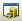
\includegraphics{images/Ex01/image2.png} на панели инструментов.

  \begin{quote}
  \textbf{Catalog (Каталог)} --- это файловый менеджер для управления
  пространственными данными. Его задачи в чем-то аналогичны Проводнику в
  Windows или Finder в Mac OS X: создание, копирование, удаление и т.д.,
  но видит она только файлы тех форматов, которые можно использовать
  в~ГИС.
  \end{quote}

  \begin{figure}
  \centering
  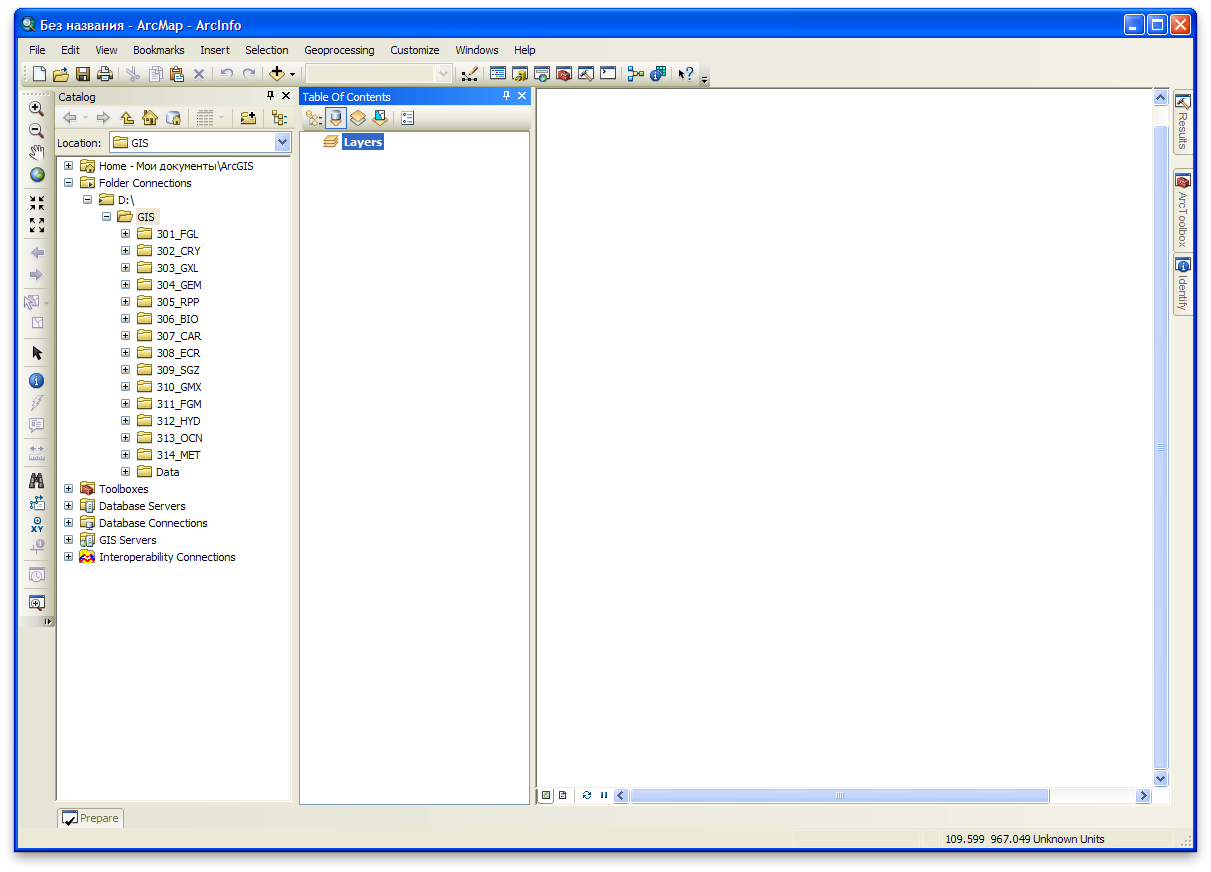
\includegraphics{images/Ex01/image3.png}
  \caption{Приложение ArcMap}
  \end{figure}
\item
  Раскройте папку \emph{D:/GIS} в дереве каталогов и найдите в ней
  директорию \emph{Ex01} в вашем каталоге, содержащую исходные данные
  для выполнения первого задания. Если директории \emph{D:/GIS} нет в
  списке, подключитесь к ней c помощью кнопки
  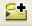
\includegraphics{images/Ex01/image4.png}.
\item
  Внутри директории \emph{Ex01} раскройте содержимое объекта под
  названием 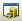
\includegraphics{images/Ex01/image5.png} \emph{Satino.gdb}
  --- это база пространственных данных, созданная в формате \emph{File
  Geodatabase} (файловая база геоданных).
\end{enumerate}

\begin{quote}
\textbf{База геоданных} --- это структурированное хранилище, внутри
которого можно создавать слои данных, группировать их и связывать
различными отношениями. В базе геоданных \emph{Satino.gdb} есть две
группы: 
\includegraphics{images/Ex01/image6.png} General
(общегеографические данные) и 
\includegraphics{images/Ex01/image6.png}
Thematic (тематические данные).
\end{quote}

Внутри базы геоданных есть данные трех типов:

\begin{itemize}
\tightlist
\item
  
\includegraphics{images/Ex01/image7.png}
\includegraphics{images/Ex01/image8.png}
\includegraphics{images/Ex01/image9.png}
  --- слои векторных данных (классы пространственных объектов),
\item
  
\includegraphics{images/Ex01/image10.png} --- слои растровых данных;
\item
  
\includegraphics{images/Ex01/image11.png} --- обычные таблицы;
\end{itemize}

\begin{quote}
\textbf{Класс пространственных объектов (feature class)} --- это набор
пространственных объектов одного типа геометрии (точки, линии, полигоны
или объемные тела). Для класса могут быть определены атрибуты, а его
представлением является таблица, содержащая как обычные столбцы
(текстовые, числовые и т.д.) так и специальное поле \emph{Shape}, в
котором хранится информация о геометрии. Каждая строчка в таблице ---
это описание одного объекта.
\end{quote}

Представьте, что вы работаете с двумя слоями: один содержит точки
наблюдений скорости течения реки Протвы, другой --- представление самой
реки на меженный уровень в виде площадного объекта. Съемка точек
производилась с помощью GPS-приемника, координаты измерены в виде
геодезических широт и долгот на эллипсоиде \emph{WGS-1984}. Береговая
линия реки получена с топографического плана и сохранена в проекции
\emph{UTM}, координаты точек границы представлены семизначными числами в
метрах.

\emph{Как совместить эти два слоя, чтобы составить карту фактического
материала?} Очевидно, надо преобразовать координаты одного слоя в
систему координат другого слоя: либо в метры в проекции UTM, либо в
градусы на эллипсоиде \emph{WGS-1984}.

\begin{enumerate}
\def\labelenumi{\arabic{enumi}.}
\item
  Дважды щелкните на слое \emph{WaterPolygon} в группе \emph{General} и
  перейдите на вкладку \textbf{XY~Coordinate System}.
\item
  Найдите строку \textbf{Projection}.

  В какой проекции хранятся координаты?

  Как вы помните, проекции обладают разными искажениями. В частности,
  проекция \emph{Меркатора} вытягивает все приполярные объекты вдоль
  меридианов, следовательно, величины плоских прямоугольных координат
  зависят о того, какая проекция используется.
\item
  Найдите строку \textbf{Linear Unit}.

  В каких единицах измерения записаны координаты в проекции слоя
  WaterPolygon? Это могут быть градусы, метры, футы (в США) и т.д.
\item
  Откройте свойства слоя \emph{HydroMeasures}, лежащего к корне базы
  геоданных. Этот слой хранится в \emph{Географической системе координат
  (ГСК)} --- широтах и долготах, отнесенных к эллипсоиду
  \emph{WGS-1984}. Т.е. у него \textbf{нет проекции}.
\item
  Закройте свойства слоя \emph{HydroMeasures}.
\item
  Перенесите в таблицу содержания слой \emph{WaterPolygon} из группы
  \emph{General}.

  Обратите внимание на то, что слой добавился под названием Гидрография
  (полигоны). У него был русскоязычный псевдоним (\emph{alias}). Его
  можно задать в свойствах слоя в \textbf{Каталоге}.

  \begin{quote}
  \textbf{Объекты базы геоданных}, такие как слои, наборы данных,
  атрибутивные поля, обычно называют латинскими буквами, однако вы
  можете дать им русскоязычные псевдонимы, которые будут отображаться
  вместо названий в \textbf{ArcMap}.
  \end{quote}
\item
  Добавьте в таблицу содержания слой \emph{HydroMeasures}. Обратите
  внимание на то, что слои совместились, несмотря на то, что у них
  различные системы координат!
\item
  Откройте панель инструментов \textbf{Tools} (инструменты), щелкнув
  правой кнопкой мыши вверху окна и выбрав ее из списка.
\item
  Попробуйте инструменты навигации с панели \textbf{Tools}:
  увеличить/уменьшить 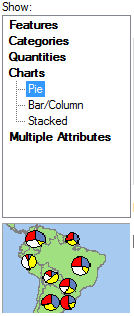
\includegraphics{images/Ex01/image12.png} и
  переместить 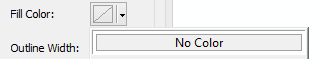
\includegraphics{images/Ex01/image13.png}. Обратите
  внимание на то, как будет меняться масштаб вверху окна.

  \begin{quote}
  Для быстрого доступа к инструментам \textbf{увеличить, уменьшить и
  переместить} используйте клавиши Z, X и C соответственно.
  \end{quote}
\item
  Выберите инструмент 
\includegraphics{images/Ex01/image14.png}
  \textbf{Identify} и щелкните мышью на любом объекте, либо растяните
  прямоугольник вокруг объектов.

  Какую информацию позволяет узнать инструмент идентификации?
\item
  Откройте атрибутивную таблицу слоя \emph{Гидрография (полигоны)},
  щелкнув на нем правой кнопкой мыши и выбрав команду \textbf{Open
  Attribute Table}.
\item
  Найдите поля \emph{Shape} и \emph{ObjectID}.

  \begin{quote}
  \textbf{Звездочка} (*) рядом с названием поля означает, что для него
  внутри базы геоданных построен \emph{индекс} --- невидимая
  вспомогательная таблица, позволяющая быстро находить объекты по их
  атрибутам или местоположению. Соответственно, различают атрибутивный и
  пространственный индекс.
  \end{quote}

  В поле \emph{ObjectID} хранится уникальный идентификатор каждого
  объекта. Он нужен системе для того, чтобы каждый объект можно было
  гарантированно найти по некому однозначному критерию.

  В поле \emph{Shape} (вспомните, что слой полигональный) хранится
  список координат вершин полигона. Геометрия объектов редактируется
  специальными инструментами, поэтому содержимое поля \emph{Shape}
  скрыто от пользователя.
\item
  Закройте атрибутивную таблицу.
\end{enumerate}

\hypertarget{map-design-quaternary-representations}{%
\section{Способы
изображения}\label{map-design-quaternary-representations}}

\protect\hyperlink{map-design-quaternary}{В начало упражнения ⇡}

\textbf{Карта} --- язык географии, и квалифицированный географ должен
уметь пользоваться современным диалектом этого языка. В основе языка
карт, как вы помните, лежат символы и способы изображения.

\begin{enumerate}
\def\labelenumi{\arabic{enumi}.}
\item
  Удалите из таблицы содержания слой \emph{HydroMeasures} и добавьте
  слой \emph{QDeposit} (четвертичные отложения). Перетащите его вниз
  списка и дважды щелкните на нем.
\item
  Перейдите на вкладку \textbf{Symbology}. Здесь вы встретите многие
  знакомые вам способы изображения.

  Просмотрите список в левой части диалога и попробуйте назвать способы
  изображения, основываясь на вспомогательных иллюстрациях. Обсудите их
  с преподавателем.

  Четвертичные отложения показываются качественным фоном. В ArcGIS этот
  способ изображения называется \textbf{Categories} (категории).
\item
  Выберите пункт \textbf{Categories} в списке слева, и в нем же выберите
  режим \emph{Unique values} (уникальные значения).

  Вверху вы должны увидеть два списка: поле, из которого необходимо
  взять уникальные значения, и цветовая шкала.
\item
  Выберите поле \emph{Отложения} в списке \textbf{Value Field}, и
  нажмите внизу диалога кнопку \textbf{Add All Values}. Программа
  просканирует всем строчкитаблицы, найдет уникальные значения, которые
  там есть, и подставит их в список. В крайнем правом поле отображается
  количество объектов каждого уникального значения:

  \begin{figure}
  \centering
  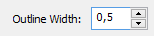
\includegraphics{images/Ex01/image15.png}
  \caption{Диалог настройки способа изображения}
  \end{figure}

  Обратите внимание на то, что типам объектов были автоматически
  присвоены символы из той цветовой шкалы, которая выбрана справа
  вверху.
\item
  Снимите галочку \textbf{All other values}, расположенную вверху
  списка.
\item
  Разверните список цветовых шкал \textbf{Color Ramp} и выберите любую
  другую на свой вкус. Цвета объектов в легенде автоматически
  поменяются.

  Вы помните, однако, что есть официальные и неофициальные
  договоренности относительно цветов, используемых на геологических,
  геоморфологических, почвенных, геоботанических картах. Вы можете
  задать каждому типу индивидуально тот цвет, который требуется. Более
  того, вы можете сохранить набор цветов как шкалу.
\item
  Щелкните дважды на любом символе в легенде. Перед вами появится диалог
  настройки символа, в котором вы можете поэкспериментировать.
\item
  Закройте диалог настройки символа и нажмите \textbf{ОК} в диалоге
  свойств слоя.
\end{enumerate}

Теперь слой \emph{Четвертичные отложения} показан методом качественного
фона с использованием тех цветов, которые были назначены каждому типу.

\hypertarget{map-design-quaternary-labels}{%
\section{Подписи}\label{map-design-quaternary-labels}}

\protect\hyperlink{map-design-quaternary}{В начало упражнения ⇡}

В предыдущем разделе вы изучили возможные способы изображения и показали
типы рельефа методом качественного фона. Однако карты без подписей
встречаются крайне редко. Если в слое есть поле с теми значениями,
которые надо вынести в качестве подписей, это делается автоматически.

\begin{enumerate}
\def\labelenumi{\arabic{enumi}.}
\item
  Убедитесь, что включен механизм расстановки подписей \textbf{Maplex}.
  Для этого откройте панель инструментов \textbf{Labeling} и поставьте
  соответствующую галочку:

  \begin{figure}
  \centering
  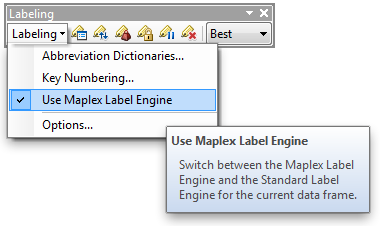
\includegraphics{images/Ex01/image16.png}
  \caption{Включение механизма расстановки подписей Maplex}
  \end{figure}
\item
  Откройте снова свойства слоя Четвертичные отложения и перейдите на
  вкладку \textbf{Labels}.
\item
  Отметьте галочкой опцию \textbf{Label features in this layer}. Эта
  опция включает подписи для слоя.
\item
  В поле \textbf{Label Field} выберите значение \emph{Индекс} Подписи
  будут браться из этого поля. Рядом расположены элементы настройки
  шрифта, с которыми вы можете поэкспериментировать:

  \begin{figure}
  \centering
  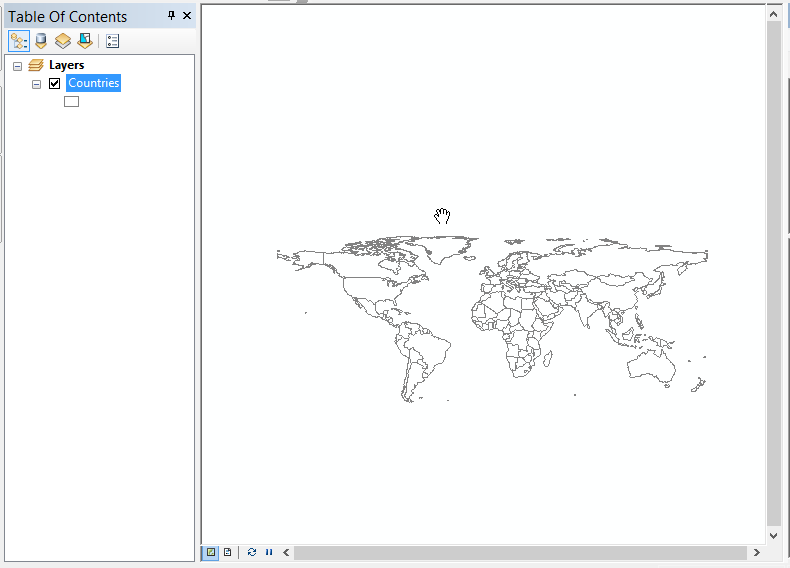
\includegraphics{images/Ex01/image17.png}
  \caption{Диалог настройки подписей для объектов}
  \end{figure}
\item
  Нажмите кнопку \textbf{Placement Properties}. Появившийся диалог
  позволяет вам настроить, как именно будут размещены подписи
  относительно самих объектов. Это очень мощный инструмент, который
  управляет множеством нюансов расстановки подписей.
\item
  В диалоге \textbf{Placement Properties} нажмите кнопку
  \textbf{Position} и изучите возможные варианты. Попробуйте применить
  разные варианты. В конце верните способ по умолчанию --- горизонтально
  внутри.
\item
  Закройте все диалоговые окна, последовательно нажимая кнопку
  \textbf{OK} в каждом из них.
\item
  Нажмите кнопку 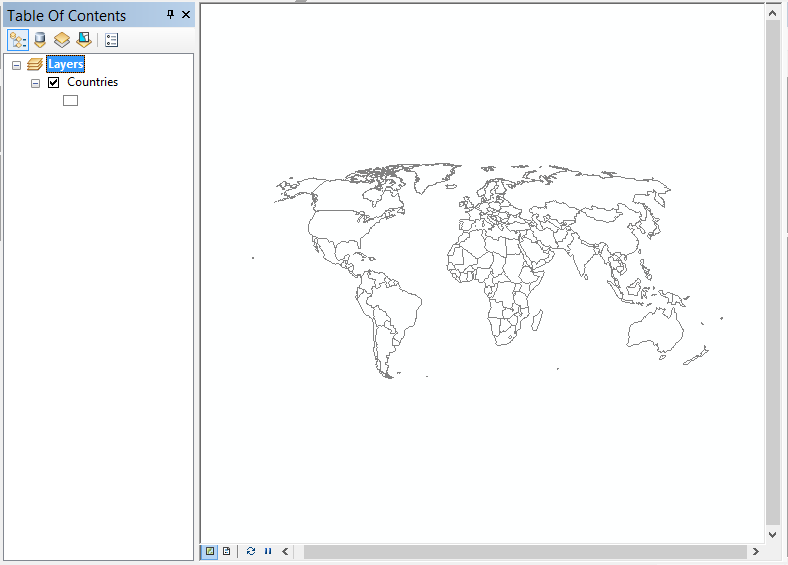
\includegraphics{images/Ex01/image18.png} на панели
  \textbf{Tools}, чтобы вся карта уместилась в окне просмотра. Окно
  приложения примет вид, примерно соответствующий тому, что показано на
  рисунке ниже:

  \begin{figure}
  \centering
  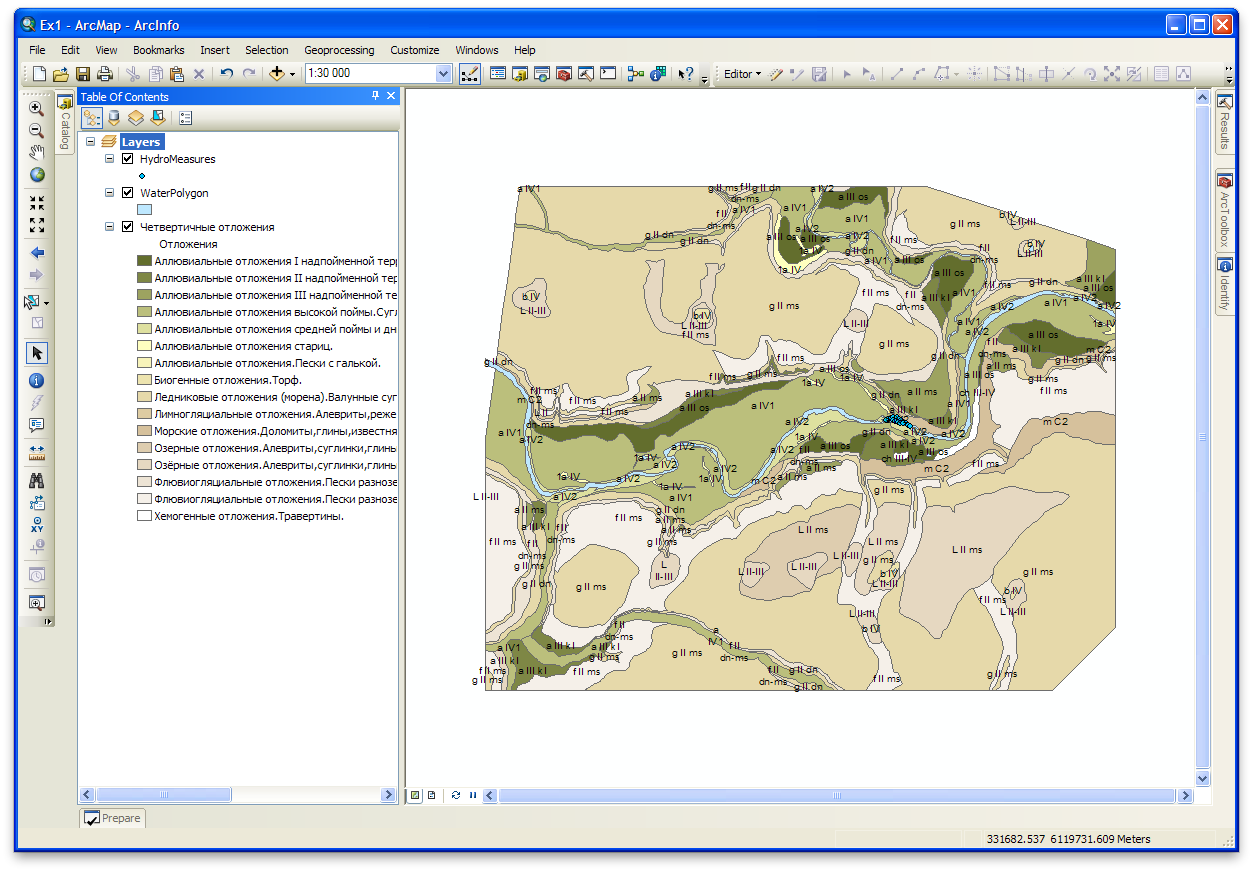
\includegraphics{images/Ex01/image19.png}
  \caption{Карта четвертичных отложений с индексами в произвольной
  цветовой шкале}
  \end{figure}
\end{enumerate}

Обратите внимание, что на вашей карте все объекты подписаны одинаково.
Если требуется, чтобы подписи объектов были разными в зависимости от
типа объекта, на вкладке \textbf{Labels} свойств слоя необходимо сменить
режим \emph{Label all the features the same way} на режим \emph{Define
classes\ldots{}} и произвести настройку.

\textbf{Снимок экрана №1.} Окно карты с подписями объектов

\hypertarget{map-design-quaternary-layout}{%
\section{Компоновка карты}\label{map-design-quaternary-layout}}

\protect\hyperlink{map-design-quaternary}{В начало упражнения ⇡}

Если карту необходимо подготовить к печати, снабдить заголовком,
масштабом, легендой и градусной сеткой, используется режим компоновки.

\begin{enumerate}
\def\labelenumi{\arabic{enumi}.}
\item
  Выберите пункт меню \textbf{View \textgreater{} Layout View}.
  Приложение перейдет в режим компоновки.
\item
  Откройте панель инструментов \textbf{Layout}. С ее помощью вы можете
  осуществлять навигацию в режиме компоновки:

  \begin{figure}
  \centering
  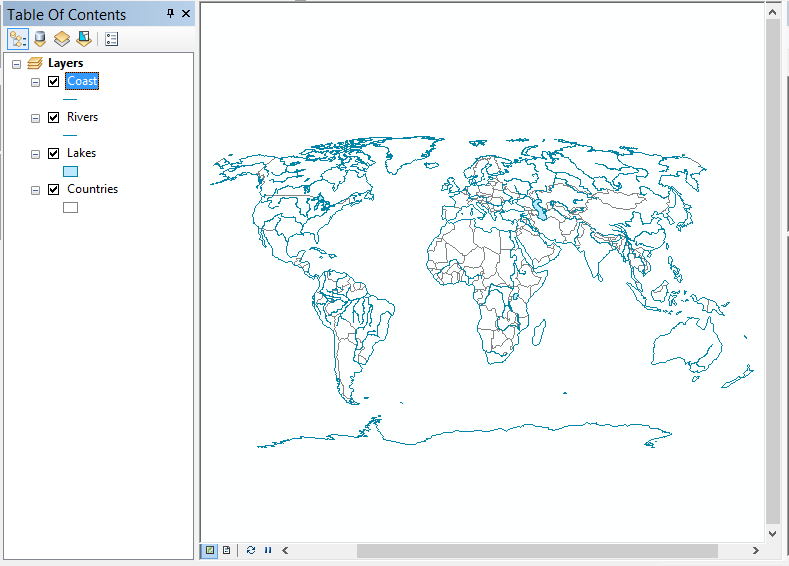
\includegraphics{images/Ex01/image20.png}
  \caption{Панель инструментов Layout}
  \end{figure}
\item
  Откройте меню \textbf{Insert} и изучите его содержание.

  Обсудите с преподавателем, какие элементы компоновки можно создать.
\item
  Вставьте название карты (\textbf{Insert \textgreater{} Title}). В
  появившемся диалоге введите текст «Карта четвертичных отложений».
  Сдвиньте название в угол листа.
\item
  Вставьте легенду (\textbf{Insert \textgreater{} Legend}). Добавьте
  туда только слой четвертичных отложений. Разберитесь самостоятельно с
  мастером создания легенды.

  Настройка легенды разнесена на несколько диалоговых окон. Изучите
  назначение каждого из них. Обсудите их с преподавателем.

  Сетка прямоугольных координат строго привязана к местоположению самой
  карты, поэтому она является ее свойством. Для того, чтобы вставить ее,
  выполните следующие шаги:
\item
  Дважды щелкните на заголовке фрейма данных \textbf{Layers} и перейдите
  на вкладку \textbf{Grid}.
\item
  Нажмите кнопку \textbf{New Grid}.

  Перед вами окажется диалог с тремя типами возможных сеток. Чем они
  отличаются? Обсудите их с преподавателем.
\item
  Выберите режим \emph{Measured Grid}, который создает сетку в плоских
  прямоугольных координатах. Изучите модерждание каждого последующего
  диалога, параметры оставьте по умолчанию
\item
  Нажмите \textbf{ОК} в свойствах фрейма данных. Теперь поверх вашей
  карты должна отображаться сетка прямоугольных координат.
\item
  Разместите на карте линейный масштаб в метрах.
\end{enumerate}

\textbf{Снимок экрана №2.} Компоновка карты с легендой и масштабом

Сохраните карту через команду меню \textbf{File \textgreater{} Save~as}
в свою директорию под названием \emph{Ex01.mxd}.

\hypertarget{map-design-quaternary-attributes}{%
\section{Редактирование
атрибутов}\label{map-design-quaternary-attributes}}

\protect\hyperlink{map-design-quaternary}{В начало упражнения ⇡}

Атрибуты играют важную роль в геоинформационных системах. На их основе
происходит визуализация данных, также они участвуют в большинстве
операций пространственного анализа. Необходимо овладеть техникой их
создания, редактирования и использования.

Редактирование атрибутов может понадобиться при заполнении полей для
новых объектов, исправлении ошибок и заполнении пустых значений.

\begin{enumerate}
\def\labelenumi{\arabic{enumi}.}
\item
  Переключитесь обратно в режим \textbf{View \textgreater{} Data View}.
\item
  Добавьте на карту слой 
\includegraphics{images/Ex01/image8.png}
  \emph{WaterLine} (линейные объекты гидрографии).
\item
  Исправьте его символ на голубую линию толщиной 1.5 пиксела, чтобы он
  лучше читался на карте.
\item
  Включите подписи по полю \emph{RiverName} на вкладке \textbf{Labels},
  задайте им синий цвет, криволинейное размещение и нажмите \textbf{OK}
  в диалоге свойств слоя.

  Появились ли подписи ручьев?

  По всей видимости, с полем \emph{RiverName} что-то не в порядке.
  Давайте проинспектируем атрибутивную таблицу.
\item
  Зажмите клавишу Ctrl и дважды кликните на названии слоя
  \emph{Гидрография (линии)}. Откроется его атрибутивная таблица.

  \begin{quote}
  Таблицу также можно открыть через контекстное меню слоя, выбрав пункт
  \textbf{Open Attribute Table}. Свойства слоя также доступны из пункта
  \textbf{Properties} в контекстном меню. Однако вариант с двойным
  нажатием более быстрый и, скорее всего, более удобный.
  \end{quote}

  Похоже, что создатель слоя забыл внести в него названия водотоков.
  Следует исправить этот недочет.
\item
  Пристыкуйте таблицу в нижнюю часть окна, чтобы она не загораживала
  карту.
\item
  Выделите в таблице содержания слой Гидрография (линии) и в его
  контекстном меню выберите пункт
  \textbf{Edit~Features~\textgreater{}~Start~Editing}. Включится режим
  редактирования, который позволяет вручную править атрибуты и геометрию
  объектов. Должна появиться панель редактора:

  \begin{figure}
  \centering
  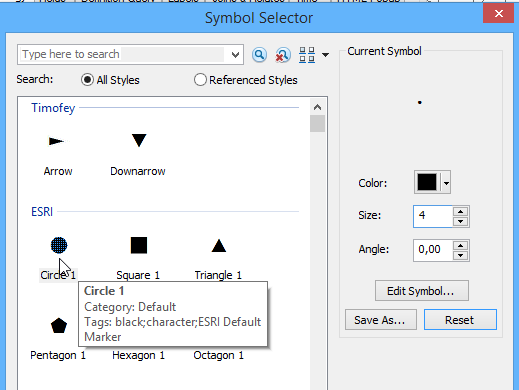
\includegraphics{images/Ex01/image21.png}
  \caption{Панель редактирования Editor}
  \end{figure}
\item
  Чтобы не выделять лишних объектов, в контекстном меню слоя
  \emph{Гидрография (линии)} выберите пункт \textbf{Selection
  \textgreater{} Make this the only selectable layer}
\item
  Возьмите с панели редактора инструмент выбора (отмечен на рисунке) и
  выделите с его помощью ручей \emph{Язвицы} (на севере полигона). Он
  автоматически подсветится в таблице. Введите название в ячейку поля
  \emph{RiverName}:

  \begin{figure}
  \centering
  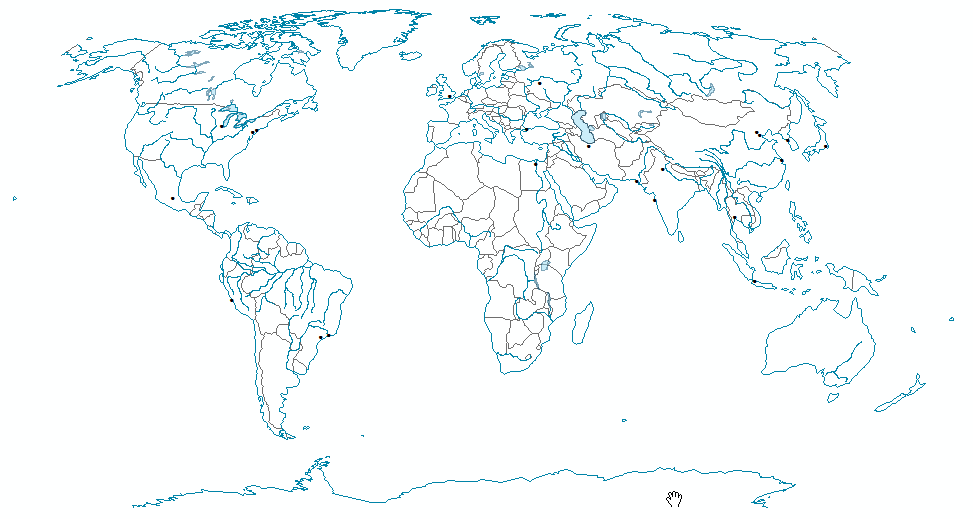
\includegraphics{images/Ex01/image22.png}
  \caption{Редактирование таблицы атрибутов слоя}
  \end{figure}
\item
  Найдите на карте Чолоховский ручей (на юге полигона), выделите его и в
  контекстном меню выберите пункт \textbf{Attributes}. Перед вами
  откроется окно редактора атрибутов --- это еще один способ
  редактирования таблицы, ориентированный на индивидуальную работу с
  каждым объектом:

  \begin{figure}
  \centering
  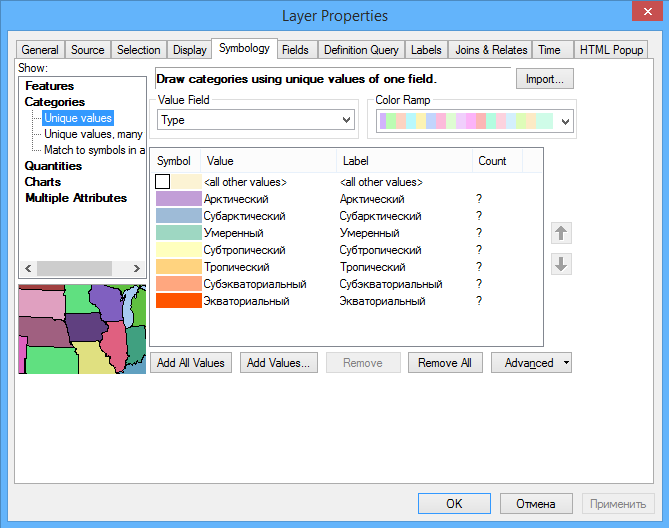
\includegraphics{images/Ex01/image23.png}
  \caption{Редактор атрибутов}
  \end{figure}
\item
  Найдите поле \emph{RiverName} и введите название ручья.
\item
  Завершите редактирование, выбрав на панели редактора пункт меню
  \textbf{Editor \textgreater{} Stop Editing}. В появившемся диалоге
  нажмите Да.
\end{enumerate}

Появились ли теперь подписи ручьев Язвицы и Чолоховский?

\textbf{Снимок экрана №3.} Окно карты с подписями ручьев

Сохраните документ карты еще раз. Сохраните ваш отчетный файл и положите
его в сетевую папку преподавателя.

\hypertarget{map-design-quaternary-calculation}{%
\section{Создание и вычисление атрибутов
(дополнительно)}\label{map-design-quaternary-calculation}}

\protect\hyperlink{map-design-quaternary}{В начало упражнения ⇡}

Поля можно не только заполнять вручную, их можно вычислять и копировать
значения из других полей. Но для начала необходимо научиться их
создавать.

Предположим, что бригада топографов произвела съемку границы леса в
целях ее сравнения с данными 10-летней давности. Чтобы построить карту
границы леса и совместить ее с другими данными, необходимо знать
координаты опорных геодезических пунктов, которые участвовали в
планово-высотном обосновании. Эти пункты есть в базе геоданных
\emph{Satino.gdb}.

\begin{enumerate}
\def\labelenumi{\arabic{enumi}.}
\item
  Добавьте на карту слой 
\includegraphics{images/Ex01/image7.png}
  \emph{GeoPoints} (геодезические пункты).
\item
  Смените через свойства слоя значок на белый треугольник с точкой
  посередине (он есть в библиотеке).
\item
  Откройте атрибутивную таблицу слоя.

  Есть ли координаты точек в таблице слоя Геодезические пункты? В каком
  поле они должны храниться?

  Координаты объектов точечного слоя можно вывести в числовое поле. Для
  этого создадим два поля \emph{X} и \emph{Y}.
\item
  Выберите в окне таблицы пункт меню
  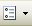
\includegraphics{images/Ex01/image24.png}
  \textbf{Table~Options~---~Add~Field\ldots{}}.
\item
  В диалоге введите \emph{X} (латиницей) в название поля \textbf{Name}.
\item
  Теперь необходимо задать тип поля. Раскройте ниспадающий список
  \textbf{Type}.

  Какой тип должно иметь поле для хранения координат геодезических
  пунктов и почему? Обсудите с преподавателем все варианты, которые есть
  в списке и случаи, когда их необходимо использовать.
\item
  Установите тип поля \emph{Float}. Остальные параметры оставьте по
  умолчанию. Нажмите \textbf{OK}.
\item
  Повторите операцию, создав поле \emph{Y}.
\item
  Нажмите правой кнопкой на заголовке поля \emph{X} и выберите в
  контекстном меню \textbf{Calculate Geometry\ldots{}}.
\item
  В появившемся диалоге из ниспадающего списка выберите величину
  \emph{X~Coordinate of Point} и единицы измерения \emph{Meters}.

  Обратите внимание, что инструмент \textbf{Calculate Geometry}
  позволяет вам вычислять координаты не только в проекции данных
  (\emph{data source}), но и в проекции карты (\emph{data frame}).
\item
  Нажмите \textbf{OK}.
\item
  Повторите вычисление координаты для поля \textbf{Y}

  Какого порядка величины получились в полях \textbf{X} и \textbf{Y}?
  Вспомните, куда направлена ось \emph{X} в проеции
  \emph{UTM/Гаусса-Крюгера}. Нет ли здесь противоречия?

  \begin{quote}
  В ArcGIS используется стандартная система плоских прямоугольных
  координат, в которой ось \emph{X} направлена на восток, а ось \emph{Y}
  --- на север. То же самое касается и проекций Гаусса-Крюгера и UTM
  \end{quote}
\end{enumerate}

\hypertarget{map-design-quaternary-questions}{%
\section{Контрольные вопросы}\label{map-design-quaternary-questions}}

\protect\hyperlink{map-design-quaternary}{В начало упражнения ⇡}

\begin{enumerate}
\def\labelenumi{\arabic{enumi}.}
\item
  Какие типы геометрии допустимы для слоев в базе геоданных?
\item
  Что хранят системные поля Shape и ObjectID?
\item
  Если у слоя нет проекции, то в какой системе координат он хранится и в
  каких единицах измерения выражены координаты?
\item
  Как добавить слой базы данных на карту в ArcMap? Опишите
  последовательность действий.
\item
  Как получить доступ к настройкам отображения слоя? Опишите
  последовательность действий.
\item
  Чем отличается вид компоновки от вида данных?
\item
  Какая команда меню позволяет создать легенду?
\item
  Если открыта таблица слоя, что нужно включить, чтобы отредактировать
  значение в ячейке?
\end{enumerate}

\hypertarget{map-design-general}{%
\chapter{Создание общегеографической карты}\label{map-design-general}}

\hypertarget{map-design-general-intro}{%
\section{Введение}\label{map-design-general-intro}}

\textbf{Цель задания} --- знакомство с моделями пространственных
объектов и базой пространственных данных. Визуализация данных на карте.
Оформление легенды и компоновки карты.

\begin{longtable}[]{@{}ll@{}}
\toprule
Параметр & Значение\tabularnewline
\midrule
\endhead
\emph{Теоретическая подготовка} & Модели пространственных данных, модели
пространственных объектов, базы пространственных объектов,
картографические проекции\tabularnewline
\emph{Практическая подготовка} & Не требуется\tabularnewline
\emph{Исходные данные} & Картографическая база данных на территорию
Швейцарии\tabularnewline
\emph{Результат} & Общегеографическая карта Швейцарии в масштабе 1:1 750
000.\tabularnewline
\emph{Ключевые слова} & Модели пространственных данных, модели
пространственных объектов, базы пространственных данных, классы
пространственных объектов, визуализация пространственных
данных\tabularnewline
\bottomrule
\end{longtable}

\hypertarget{map-design-general-control}{%
\subsection{Контрольный лист}\label{map-design-general-control}}

\begin{itemize}
\tightlist
\item
  Добавить на карту слои базы пространственных данных и оформить их
\item
  Настроить подписи объектов
\item
  Создать компоновку карты и легенду
\item
  Экспортировать результат в графический файл
\end{itemize}

\hypertarget{map-design-general-annotation}{%
\subsection{Аннотация}\label{map-design-general-annotation}}

Задание посвящено знакомству с созданием тематических карт на основе баз
пространственных данных. Вы познакомитесь с представлением площадных,
линейных, точечных объектов в базе пространственных данных. Научитесь
создавать карты на их основе, оформлять легенду, сетку координат и
зарамочные элементы карты.

\hypertarget{map-design-general-begin}{%
\section{Начало работы}\label{map-design-general-begin}}

\protect\hyperlink{map-design-general}{В начало упражнения ⇡}

\begin{enumerate}
\def\labelenumi{\arabic{enumi}.}
\item
  Запустите приложение \textbf{ArcMap} и откройте окно \textbf{Сatalog}
\item
  Подключитесь к рабочему каталогу \emph{Ex02} в окне \textbf{Сatalog}.

  В каталоге \emph{Ex02} находится база геоданных \emph{MapData.gdb},
  содержащая исходные данные для выполнения задания. Внутри базы
  геоданных могут быть объекты следующих типов:

  \begin{itemize}
  \tightlist
  \item
    
\includegraphics{images/Ex02/image5.png}
\includegraphics{images/Ex02/image6.png}
\includegraphics{images/Ex02/image7.png}
    --- слои векторных данных (классы пространственных объектов),
  \item
    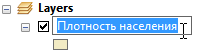
\includegraphics{images/Ex02/image8.png} --- слои растровых данных;
  \item
    
\includegraphics{images/Ex02/image9.png} --- обычные таблицы;
  \end{itemize}
\item
  Раскройте базу данных \emph{MapData.gdb} и изучите ее содержимое:

  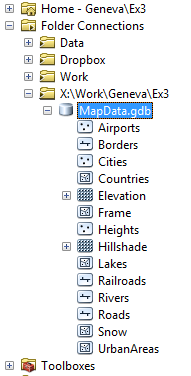
\includegraphics{images/Ex02/image10.png}
\end{enumerate}

Векторные слои базы данных \emph{MapData.gdb}:

\begin{longtable}[]{@{}ll@{}}
\toprule
Слой & Содержание\tabularnewline
\midrule
\endhead
\emph{Airports} & Аэропорты\tabularnewline
\emph{Borders} & Границы\tabularnewline
\emph{Cities} & Города\tabularnewline
\emph{Countries} & Страны\tabularnewline
\emph{Frame} & Рамка (фрейм)\tabularnewline
\emph{Heights} & Высотные отметки\tabularnewline
\emph{Lakes} & Озера\tabularnewline
\emph{Railroads} & Железные дороги\tabularnewline
\emph{Rivers} & Реки\tabularnewline
\emph{Roads} & Дороги\tabularnewline
\emph{Snow} & Ледники и снежники\tabularnewline
\emph{UrbanAreas} & Урбанизированные территории\tabularnewline
\bottomrule
\end{longtable}

Растровые слои базы данных \emph{MapData.gdb}:

\begin{longtable}[]{@{}ll@{}}
\toprule
Слой & Содержание\tabularnewline
\midrule
\endhead
\emph{Elevation} & Высоты рельефа\tabularnewline
\emph{Hillshade} & Отмывка рельефа\tabularnewline
\bottomrule
\end{longtable}

\hypertarget{map-design-general-relief}{%
\section{Оформление рельефа}\label{map-design-general-relief}}

\protect\hyperlink{map-design-general}{В начало упражнения ⇡}

\begin{enumerate}
\def\labelenumi{\arabic{enumi}.}
\item
  Добавьте на карту слой \emph{Elevation} из базы данных
  \emph{MapData.gdb}.
\item
  В настройках оформления растрового слоя установите способ градиентной
  окраски со следующими параметрами:

  \begin{longtable}[]{@{}ll@{}}
  \toprule
  Параметр & Значение\tabularnewline
  \midrule
  \endhead
  \emph{Шкала} & Surface
  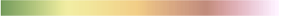
\includegraphics{images/Ex02/image11.png}\tabularnewline
  \emph{Растяжка гистограммы} & Минимум-Максимум
  (Minimum-maximum)\tabularnewline
  \bottomrule
  \end{longtable}
\item
  Установите передискретизацию слоя в режим кубической cвертки
  (\emph{Cubic Convolution}).

  \emph{Результат:} 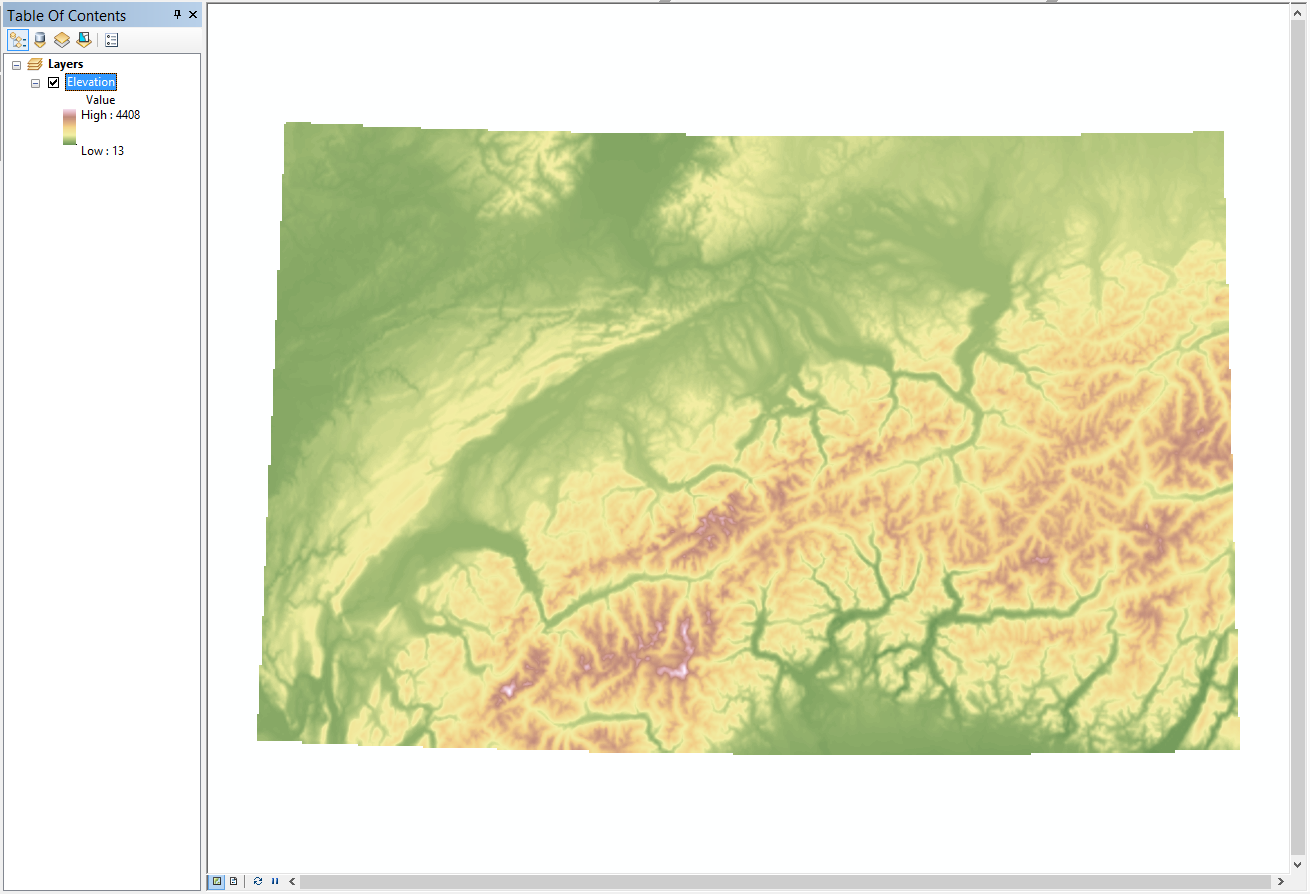
\includegraphics{images/Ex02/image12.png}
\item
  Наложите отмывку поверх гипсометрической окраски. Для этого добавьте
  на карту слой отмывки \emph{Hillshade} и установите для него следующие
  параметры:

  \begin{longtable}[]{@{}ll@{}}
  \toprule
  Параметр & Значение\tabularnewline
  \midrule
  \endhead
  \emph{Прозрачность} & 50\%\tabularnewline
  \emph{Режим передискретизации} & Кубическая свертка\tabularnewline
  \bottomrule
  \end{longtable}

  Остальные параметры оставьте по умолчанию.

  \emph{Результат}: 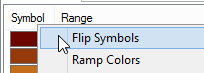
\includegraphics{images/Ex02/image13.png}
\end{enumerate}

Сохраните документ карты в каталог Ex02 под названием Ex02\_Фамилия.

\hypertarget{map-design-general-vector}{%
\section{Оформление векторных слоев}\label{map-design-general-vector}}

\protect\hyperlink{map-design-general}{В начало упражнения ⇡}

Добавьте на карту и оформите векторные слои, содержащиеся в базе данных
\emph{MapData.gdb}, все кроме слоя \emph{Countries}. Для каждого слоя
выберите единый символ. В качестве образца оформления используйте
рисунок ниже. 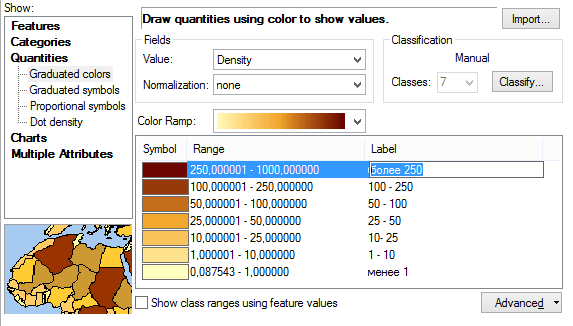
\includegraphics{images/Ex02/image14.png}

Учтите, что:

\begin{itemize}
\item
  Слой \emph{Snow} располагается между отмывкой и цветовой окраской
  рельефа. Это позволяет показать заснеженные территории, но при этом
  сохранить светотеневую пластику.
\item
  При выборе значка для аэропорта следует воспользоваться поиском по
  символам, набрав ключевое слово \emph{«airport»}
\end{itemize}

\emph{Результат}: 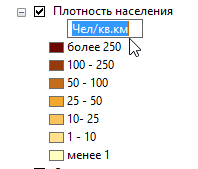
\includegraphics{images/Ex02/image15.png}

\hypertarget{map-design-general-labels}{%
\section{Создание подписей}\label{map-design-general-labels}}

\protect\hyperlink{map-design-general}{В начало упражнения ⇡}

\begin{enumerate}
\def\labelenumi{\arabic{enumi}.}
\item
  Установите масштаб карты равным 1:1~750~000.
\item
  Включите \textbf{Maplex} для размещения подписей и переведите его в
  режим \emph{Best}
\item
  Сделайте подписи для слоев \emph{Cities}, \emph{Heights},
  \emph{Rivers}, \emph{Lakes} со следующими параметрами:

  \emph{Cities}:

  \begin{longtable}[]{@{}ll@{}}
  \toprule
  Параметр & Значение\tabularnewline
  \midrule
  \endhead
  \emph{Шрифт} & Calibri\tabularnewline
  \emph{Размер} & 10\tabularnewline
  \emph{Цвет} & Черный\tabularnewline
  \emph{Начертание} & Обычный\tabularnewline
  \emph{Размещение} & По умолчанию\tabularnewline
  \emph{Образец} &
  -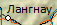
\includegraphics{images/Ex02/image16.png}\tabularnewline
  \bottomrule
  \end{longtable}

  \emph{Heights}:

  \begin{longtable}[]{@{}ll@{}}
  \toprule
  Параметр & Значение\tabularnewline
  \midrule
  \endhead
  \emph{Шрифт} & Calibri\tabularnewline
  \emph{Размер} & 7\tabularnewline
  \emph{Цвет} & Серый 80\%\tabularnewline
  \emph{Начертание} & Курсивный\tabularnewline
  \emph{Размещение} & По умолчанию\tabularnewline
  \emph{Образец} &
  -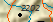
\includegraphics{images/Ex02/image17.png}\tabularnewline
  \bottomrule
  \end{longtable}

  \emph{Rivers}:

  \begin{longtable}[]{@{}ll@{}}
  \toprule
  Параметр & Значение\tabularnewline
  \midrule
  \endhead
  \emph{Шрифт} & Calibri\tabularnewline
  \emph{Размер} & 10\tabularnewline
  \emph{Цвет} & Синий Dark Navy\tabularnewline
  \emph{Начертание} & Курсивный\tabularnewline
  \emph{Размещение} & Regular Placement \textgreater{} Offset
  Curved\tabularnewline
  \emph{Образец} &
  -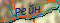
\includegraphics{images/Ex02/image18.png}\tabularnewline
  \bottomrule
  \end{longtable}

  \emph{Lakes}:

  \begin{longtable}[]{@{}ll@{}}
  \toprule
  Параметр & Значение\tabularnewline
  \midrule
  \endhead
  \emph{Шрифт} & Calibri\tabularnewline
  \emph{Размер} & 8\tabularnewline
  \emph{Цвет} & Синий Dark Navy\tabularnewline
  \emph{Начертание} & Курсивный\tabularnewline
  \emph{Размещение} & Regular Placement \textgreater{}
  Curved\tabularnewline
  \emph{Образец} &
  -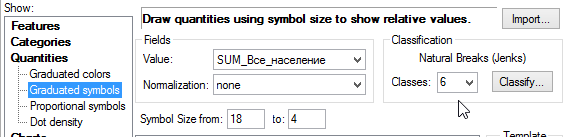
\includegraphics{images/Ex02/image19.png}\tabularnewline
  \bottomrule
  \end{longtable}
\end{enumerate}

\emph{Результат} должен выглядеть примерно следующим образом:
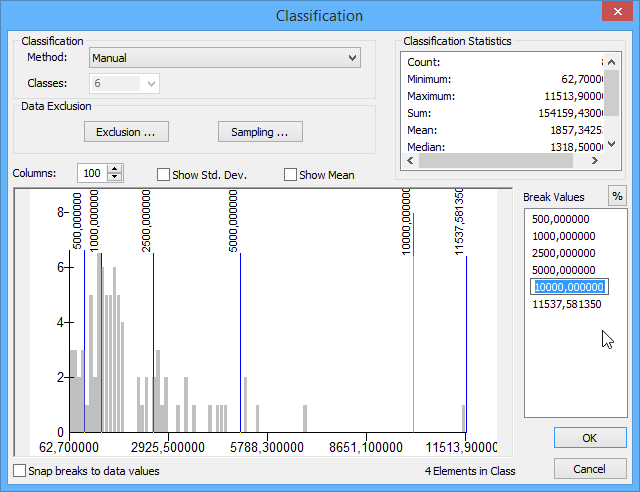
\includegraphics{images/Ex02/image20.png}

\hypertarget{map-design-general-cities}{%
\section{Классификация населенных
пунктов}\label{map-design-general-cities}}

\protect\hyperlink{map-design-general}{В начало упражнения ⇡}

Недостатком полученной карты является то, что все населенные пункты
показаны одинаково. Чтобы исправить этого, необходимо разделить их по
категориям численности населения. Для этого:

\begin{enumerate}
\def\labelenumi{\arabic{enumi}.}
\item
  В диалоге настройки символов слоя включите режим отображения
  \textbf{Categories (unique values)}, используя значения поля
  \emph{Население\_диапазон}
\item
  Отсортируйте классы численности в нужном порядке, используя стрелочки.
\item
  Настройте размер кружка таким образом, чтобы его диаметр менялся от 3
  до 7 пунктов

  \emph{Результат}: 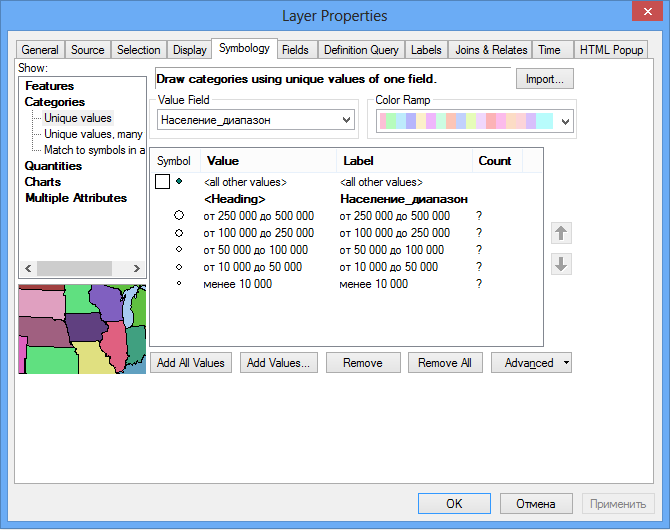
\includegraphics{images/Ex02/image21.png}
\item
  Перейдите на вкладку \textbf{Labels} и переключите подписи в режим
  нескольких классов.
\item
  Импортируйте классы с помощью кнопки \textbf{Get Symbol Classes}.
\item
  Настройте подписи следующим образом:

  \begin{itemize}
  \tightlist
  \item
    Шрифт \emph{Calibri} черного цвета
  \item
    Размер шрифта должен увеличиваться от низшего класса (менее 10 000)
    до самого крупного (от 250 000 до 500 000) с 8 до 12 пунктов.
  \item
    Подписи городов крупнее 100 000 человек должны быть жирным шрифтом.
  \end{itemize}

  \emph{Результат}: 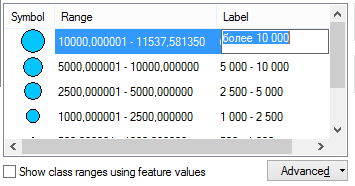
\includegraphics{images/Ex02/image22.png}
\end{enumerate}

\hypertarget{map-design-general-mask}{%
\section{Маска и подписи стран}\label{map-design-general-mask}}

\protect\hyperlink{map-design-general}{В начало упражнения ⇡}

\begin{enumerate}
\def\labelenumi{\arabic{enumi}.}
\item
  Добавьте на карту слой \emph{Countries} и расположите его между слоями
  \emph{Hillshade} и \emph{Snow}.
\item
  Настройте отображение слоя способом \textbf{Categories (unique
  values)} по полю \emph{Name}.
\item
  Установите следующие параметры отображения:

  \begin{longtable}[]{@{}ll@{}}
  \toprule
  Параметр & Значение\tabularnewline
  \midrule
  \endhead
  \emph{Цвет заливки} & Швейцария --- нет заливки, остальные страны ---
  серый 50\%\tabularnewline
  \emph{Цвет обводки} & Нет\tabularnewline
  \emph{Прозрачность слоя} & 50\%\tabularnewline
  \bottomrule
  \end{longtable}
\item
  Включите подписи стран по полю \emph{Name}, используя следующие
  параметры:

  \begin{longtable}[]{@{}ll@{}}
  \toprule
  Параметр & Значение\tabularnewline
  \midrule
  \endhead
  \emph{Шрифт} & Garamond\tabularnewline
  \emph{Размер} & 24\tabularnewline
  \emph{Цвет} & Коричневый/Бардовый\tabularnewline
  \emph{Начертание} & Обычный\tabularnewline
  \bottomrule
  \end{longtable}
\item
  Также установите следующие параметры размещения:

  \begin{longtable}[]{@{}ll@{}}
  \toprule
  Параметр & Значение\tabularnewline
  \midrule
  \endhead
  \emph{Позиция} & Type \textgreater{} Land Parcel
  Placement\tabularnewline
  \emph{Растяжка} & Распределять символы (Spread
  Characters)\tabularnewline
  \emph{Плотность размещения} & Подписывать только крупнейшую часть
  (Label largest feature part)\tabularnewline
  \emph{Разрешение конфликтов} & Никогда не удалять (Never
  Remove)\tabularnewline
  \emph{Образец} &
  -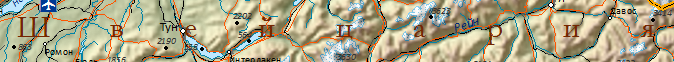
\includegraphics{images/Ex02/image23.png}\tabularnewline
  \bottomrule
  \end{longtable}
\end{enumerate}

\emph{Результат}: 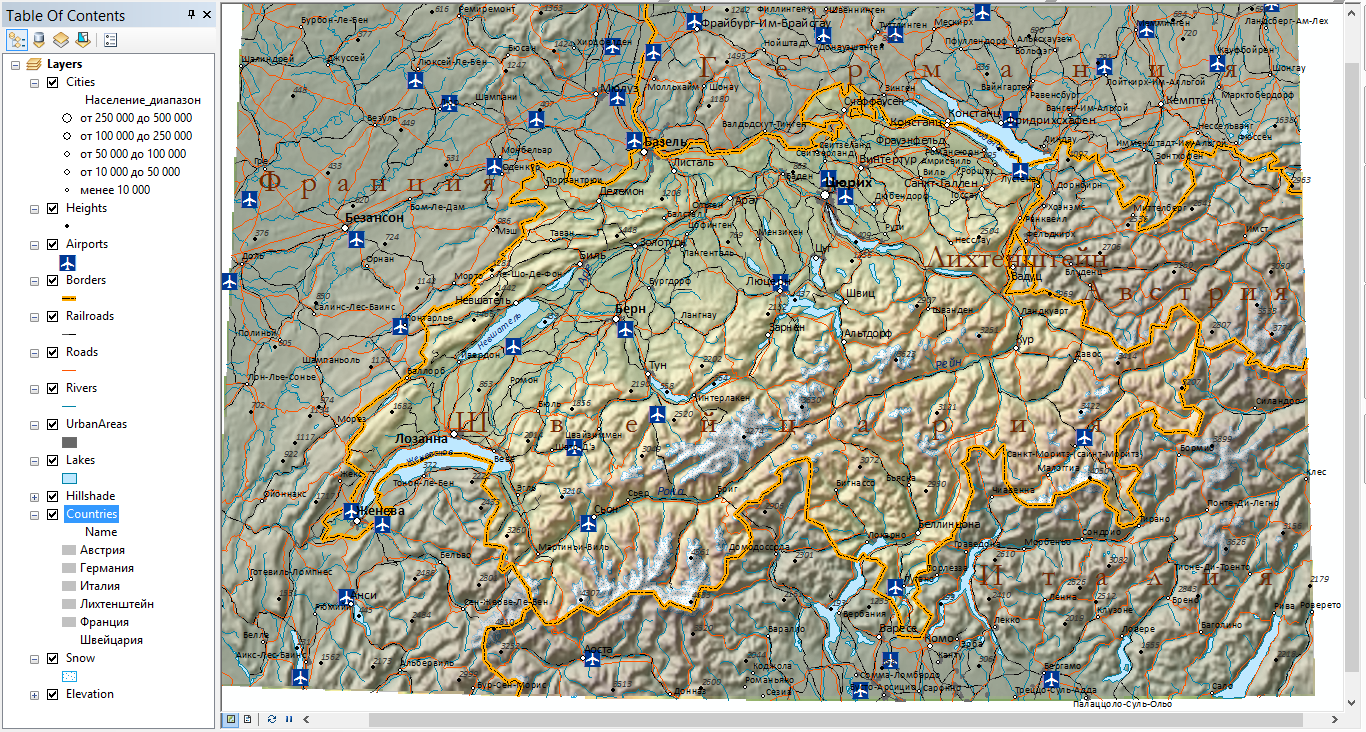
\includegraphics{images/Ex02/image24.png}

\hypertarget{map-design-general-layout}{%
\section{Настройка компоновки карты}\label{map-design-general-layout}}

\protect\hyperlink{map-design-general}{В начало упражнения ⇡}

\begin{enumerate}
\def\labelenumi{\arabic{enumi}.}
\item
  Переключитесь в вид компоновки
\item
  Настройте макет листа следующим образом:

  \begin{itemize}
  \tightlist
  \item
    Размер А4
  \item
    Альбомная ориентировка
  \end{itemize}
\item
  Подгоните размер фрейма данных таким образом, чтобы карта оказалась в
  верхней части листа
\item
  Установите масштаб равным 1:1 750 000

  \emph{Результат}: 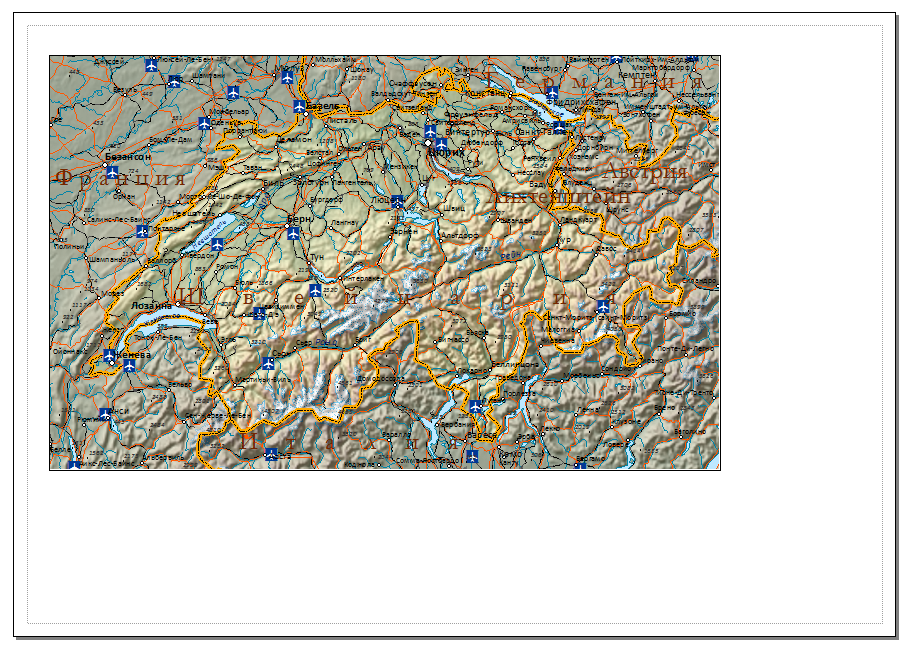
\includegraphics{images/Ex02/image25.png}
\item
  Используя настройки по умолчанию, вставьте легенду, включив в нее все
  слои, кроме \emph{Elevation}, \emph{Countries} и \emph{Hillshade}

  \emph{Результат}: 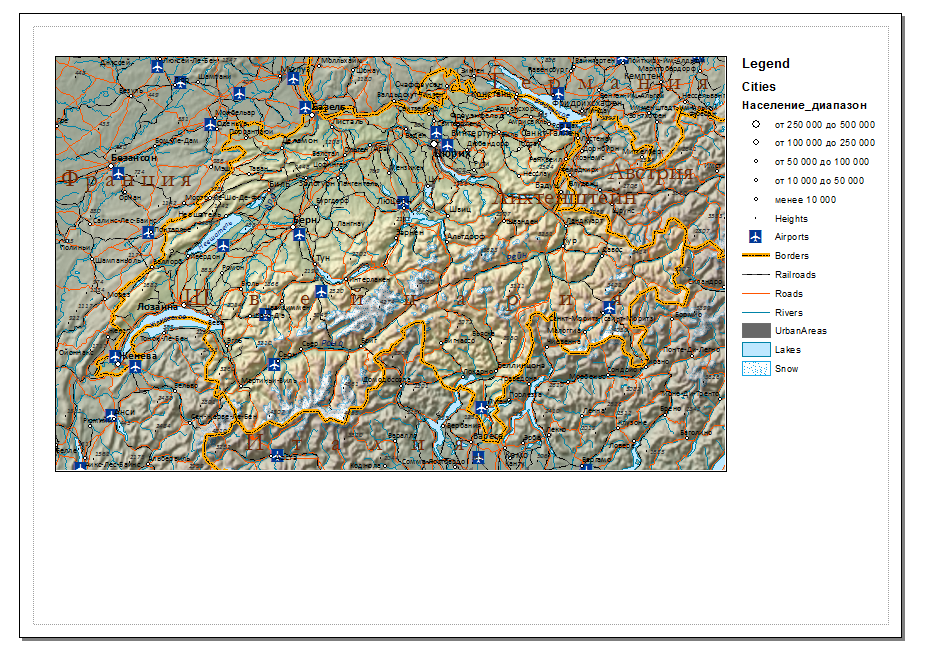
\includegraphics{images/Ex02/image26.png}
\item
  Измените название показателя для слоя \emph{Cities} на «число
  жителей». Уменьшите размер шрифта до 9 и сделайте его курсивным.
\item
  Уменьшите размер шрифта для стиля названия слоя \emph{Cities} до 10
  пунктов.
\item
  Переименуйте все слои в таблице содержания на русский язык в
  соответствии с таблицей в начале упражнения. Обратите внимание на то,
  что в легенде они переименуются автоматически.
\item
  Переименуйте заголовок легенды на русский язык.
\item
  Увеличьте интервал между слоями в легенде до 10 пунктов.

  \emph{Результат}: 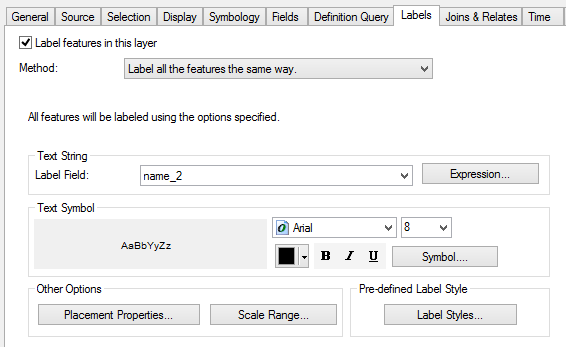
\includegraphics{images/Ex02/image27.png}
\item
  Вставьте на карту координатную сетку типа \textbf{Graticule} с шагом
  1° по широте и долготе. Отключите для градусной сетки показ минут и
  секунд.
\item
  Вставьте название карты над картой по центру, используя следующие
  параметры:

  \begin{longtable}[]{@{}ll@{}}
  \toprule
  Параметр & Значение\tabularnewline
  \midrule
  \endhead
  \emph{Шрифт} & Arial\tabularnewline
  \emph{Размер шрифта} & 16\tabularnewline
  \emph{Начертание} & Полужирный\tabularnewline
  \emph{Разрядка} & 10 пунктов\tabularnewline
  \bottomrule
  \end{longtable}
\item
  Вставьте \emph{километровую} масштабную линейку по нижеприведенному
  образцу, чтобы завершить оформление карты:

  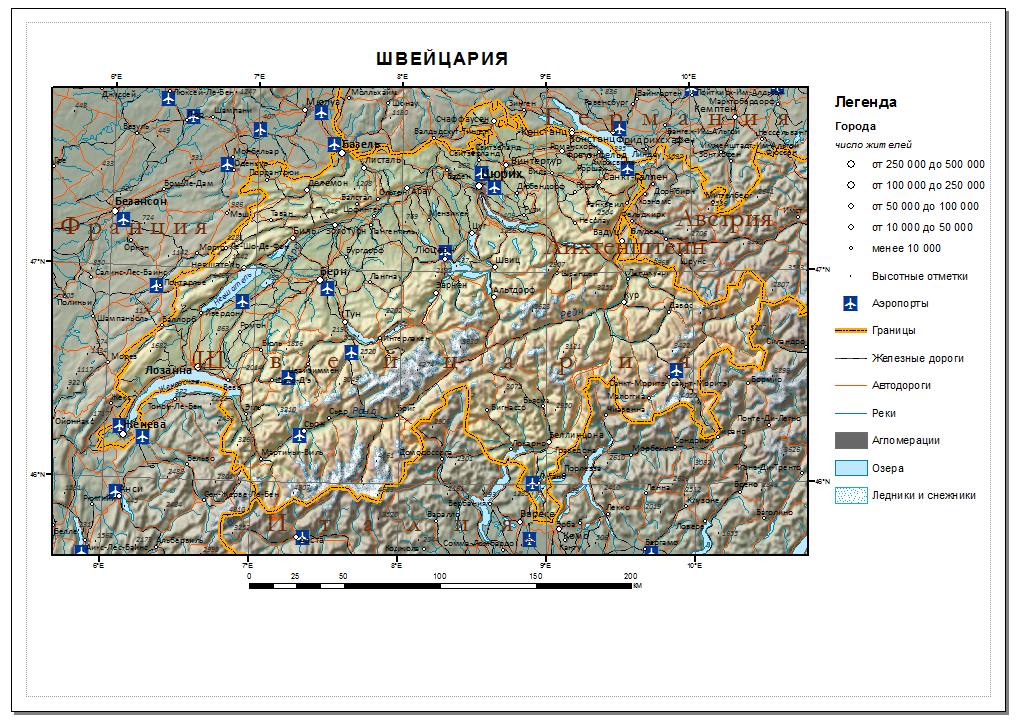
\includegraphics{images/Ex02/image28.png}
\end{enumerate}

\hypertarget{map-design-general-export}{%
\section{Экспорт в графический файл}\label{map-design-general-export}}

\protect\hyperlink{map-design-general}{В начало упражнения ⇡}

Экспортируйте карту из режима компоновки в формат PNG с разрешением 300
точек на дюйм.

\hypertarget{map-design-general-questions}{%
\section{Контрольные вопросы}\label{map-design-general-questions}}

\protect\hyperlink{map-design-general}{В начало упражнения ⇡}

\begin{enumerate}
\def\labelenumi{\arabic{enumi}.}
\item
  Какие типы геометрии допустимы для слоев в базе геоданных? К каким
  типам относятся слои, использованные вами в работе?
\item
  В какой системе координат хранились данные, которые вы использовали
  для составления карты?
\item
  Какая проекция была использована вами в работе? К какому типу по
  характеру искажений она относится?
\item
  Где хранятся данные, которые используются для классификации символов
  при отображении?
\item
  За что отвечают системные поля Shape и ObjectID?
\item
  Чем отличается вид компоновки от вида данных?
\end{enumerate}

\hypertarget{map-design-climates}{%
\chapter{Создание климатической карты}\label{map-design-climates}}

\hypertarget{map-design-climates-intro}{%
\section{Введение}\label{map-design-climates-intro}}

\textbf{Цель задания} --- знакомство с моделями пространственных
объектов и базой пространственных данных. Визуализация данных на карте.
Оформление легенды и компоновки карты.

\begin{longtable}[]{@{}ll@{}}
\toprule
Параметр & Значение\tabularnewline
\midrule
\endhead
\emph{Теоретическая подготовка} & Не требуется\tabularnewline
\emph{Практическая подготовка} & Модели пространственных данных, модели
пространственных объектов, базы пространственных объектов,
картографические проекции\tabularnewline
\emph{Исходные данные} & Климатические пояса по Алисову (полигональный
слой), границы морей и океанов IHO (International Hydrographic
Organization), направления основных течений OSCAR (Ocean Surface Current
Analyses -- Real time), крупнейшие мировые реки и озера, города (данные
Esri).\tabularnewline
\emph{Результат} & Тематическая карта «Климат и основные объекты
гидросферы» масштаба 1:90 000 000\tabularnewline
\emph{Ключевые слова} & Модели пространственных данных, модели
пространственных объектов, базы пространственных данных, классы
пространственных объектов, визуализация пространственных данных,
геоинформационное картографирование\tabularnewline
\bottomrule
\end{longtable}

\hypertarget{map-design-climates-control}{%
\subsection{Контрольный лист}\label{map-design-climates-control}}

\begin{itemize}
\tightlist
\item
  Добавить на карту слои базы пространственных данных и оформить их
\item
  Настроить подписи объектов
\item
  Создать компоновку карты, легенду и координатную сетку
\item
  Экспортировать результат в графический файл
\end{itemize}

\hypertarget{map-design-climates-annotation}{%
\subsection{Аннотация}\label{map-design-climates-annotation}}

Задание посвящено знакомству с созданием тематических карт на основе баз
пространственных данных. Вы познакомитесь с представлением площадных,
линейных, точечных объектов в базе пространственных данных. Научитесь
создавать карты на их основе, оформлять легенду, сетку координат и
зарамочные элементы карты.

\hypertarget{map-design-climates-begin}{%
\section{Начало работы}\label{map-design-climates-begin}}

\protect\hyperlink{map-design-climates}{В начало упражнения ⇡}

В каталоге \emph{Ex03} находится база геоданных \emph{Ex03.gdb},
содержащая исходные данные для выполнения задания.

\begin{quote}
\textbf{База геоданных} --- это структурированное хранилище, внутри
которого можно создавать слои данных, группировать их и связывать
различными отношениями.
\end{quote}

Внутри базы геоданных могут быть объекты следующих типов:

\begin{itemize}
\tightlist
\item
  \includegraphics{images/Ex03/image7.png}\includegraphics{images/Ex03/image8.png}\includegraphics{images/Ex03/image9.png}
  --- слои векторных данных (классы пространственных объектов),
\item
  \includegraphics{images/Ex03/image10.png} --- слои растровых данных;
\item
  \includegraphics{images/Ex03/image11.png} --- обычные таблицы;
\end{itemize}

\begin{quote}
\textbf{Класс пространственных объектов (feature class)} --- это набор
пространственных объектов одного типа геометрии (точки, линии, полигоны
или объемные тела). Для класса могут быть определены атрибуты, а его
представлением является таблица, содержащая как обычные столбцы
(текстовые, числовые и т.д.) так и специальное поле Shape, в котором
хранится информация о геометрии. Каждая строчка в таблице --- это
описание одного объекта.
\end{quote}

\begin{enumerate}
\def\labelenumi{\arabic{enumi}.}
\item
  Запустите приложение \textbf{ArcMap} и откройте окно \textbf{Catalog},
  нажав кнопку \includegraphics{images/Ex03/image5.png} на панели
  инструментов
\item
  Раскройте папку \emph{D:/GIS} в дереве каталогов и найдите в ней
  директорию \emph{Ex03} в вашем каталоге, содержащую исходные данные
  для выполнения первого задания. Если директории \emph{D:/GIS} нет в
  списке, подключитесь к ней c помощью кнопки
  \includegraphics{images/Ex03/image6.png}.
\item
  Раскройте базу данных \emph{MapData.gdb} и изучите ее содержимое,
  состоящее из следующих классов:

  \begin{longtable}[]{@{}ll@{}}
  \toprule
  \textbf{Класс} & \textbf{Содержание}\tabularnewline
  \midrule
  \endhead
  \emph{Cities} & Города\tabularnewline
  \emph{Climates} & Климатические зоны\tabularnewline
  \emph{Coast} & Побережье\tabularnewline
  \emph{Countries} & Страны\tabularnewline
  \emph{Currents} & Данные о течениях\tabularnewline
  \emph{Lakes} & Озера\tabularnewline
  \emph{Rivers} & Крупнейшие реки\tabularnewline
  \emph{Seas} & Моря\tabularnewline
  \bottomrule
  \end{longtable}

  К какому типу геометрии относятся данные классы?
\item
  Дважды щелкните на слое \emph{Climates} и перейдите на вкладку XY
  Coordinate System.
\end{enumerate}

Внимательно прочитайте информацию. Этот слой хранится в
\emph{Географической системе координат (GCS)}, отнесенной к эллипсоиду
WGS-1984. Это означает, что координаты каждого объекта хранятся в виде
широты и долготы. В любой момент этот слой можно спроецировать в любую
проекцию. При этом координаты будут представлены в метрических единицах,
а система координат получит название \emph{Проецированной системы
координат (PCS)}.

\hypertarget{map-design-climates-layers}{%
\section{Оформление слоев}\label{map-design-climates-layers}}

\protect\hyperlink{map-design-climates}{В начало упражнения ⇡}

\begin{enumerate}
\def\labelenumi{\arabic{enumi}.}
\item
  Добавьте на карту слой \emph{Countries}, просто перетащив его из окна
  каталога.
\item
  Дважды щелкните на названии слоя \emph{Countries} и перейдите на
  вкладку Symbology.
\item
  Внимательно изучите список способов изображения слева. Они разделены
  на категории \textbf{Features} (единый символ), \textbf{Categories}
  (качественные характеристики), \textbf{Quantities} (количественные
  характеристики), \textbf{Charts} (картодиаграммы), \textbf{Multiple
  Attributes} (способы изображения по нескольким атрибутам).Разверните
  каждую группу и щелкните на каждом способе. Сопоставьте их с
  традиционной классификацией способов изображения:

  \includegraphics{images/Ex03/image12.png}
\item
  Выберите способ единого символа (\textbf{Features \textgreater{}
  Single symbol})
\item
  Щелкните на кнопке с изображением символа и измените оформление
  следующим образом:

  \begin{longtable}[]{@{}ll@{}}
  \toprule
  \textbf{Параметр} & \textbf{Значение}\tabularnewline
  \midrule
  \endhead
  \emph{Цвет заливки (Fill Color)} & Без заливки
  \includegraphics{images/Ex03/image13.png}\tabularnewline
  \emph{Цвет обводки (Outline Color)} & Серый 50\%
  \includegraphics{images/Ex03/image14.png}\tabularnewline
  \emph{Толщина обводки (Outline width)} & 0,5
  \includegraphics{images/Ex03/image15.png}\tabularnewline
  \bottomrule
  \end{longtable}

  Диалог свойств слоя:

  \includegraphics{images/Ex03/image16.png}

  Результат:

  \includegraphics{images/Ex03/image17.png}
\item
  Измените проекцию карты на \emph{проекцию Робинсона (Robinson)}. Ее
  можно найти в группе \textbf{Projected Сoordinate Systems
  \textgreater{} World}. Обратите внимание на то, как изменятся
  очертания объектов:

  \includegraphics{images/Ex03/image18.png}
\item
  Добавьте на карту слой \emph{Coast}, расположите его поверх слоя
  \emph{Countries} и измените цвет линии на \emph{Delft Blue:}

  \includegraphics{images/Ex03/image19.png}
\item
  Добавьте на карту слой \emph{Rivers} расположите его поверх слоя
  \emph{Coast} и измените цвет линии на \emph{Delft Blue,} а толщину
  сделайте равной 0,5 пиксела\emph{.}
\item
  Добавьте на карту слой \emph{Lakes}, расположите его поверх слоя
  \emph{Rivers} и измените его оформление следующим образом:

  \begin{longtable}[]{@{}ll@{}}
  \toprule
  \textbf{Параметр} & \textbf{Значение}\tabularnewline
  \midrule
  \endhead
  \emph{Цвет заливки} & Sodalite Blue\tabularnewline
  \emph{Цвет обводки} & Delft Blue\tabularnewline
  \emph{Толщина обводки} & 0,5\tabularnewline
  \bottomrule
  \end{longtable}

  Результат:

  \includegraphics{images/Ex03/image20.png}
\item
  Сохраните карту в свою директорию \emph{Ex03}.
\item
  Добавьте на карту слой \emph{Cities}, расположите его поверх слоя
  \emph{Lakes} и измените его параметры следующим образом:

  \begin{longtable}[]{@{}ll@{}}
  \toprule
  \textbf{Параметр} & \textbf{Значение}\tabularnewline
  \midrule
  \endhead
  \emph{Символ} & Circle 1\tabularnewline
  \emph{Цвет} & Черный\tabularnewline
  \emph{Размер} & 4\tabularnewline
  \bottomrule
  \end{longtable}

  \includegraphics{images/Ex03/image21.png}
\item
  Добавьте на карту слой \emph{Seas}, расположите его внизу таблицы
  содержания и измените его параметры следующим образом:

  \begin{longtable}[]{@{}ll@{}}
  \toprule
  \textbf{Параметр} & \textbf{Значение}\tabularnewline
  \midrule
  \endhead
  \emph{Цвет заливки} & Нет заливки\tabularnewline
  \emph{Цвет обводки} & Серый 50\%\tabularnewline
  \emph{Толщина обводки} & 0,5\tabularnewline
  \emph{Прозрачность} & 50\%\tabularnewline
  \bottomrule
  \end{longtable}

  Результат:

  \includegraphics{images/Ex03/image22.png}
\item
  Добавьте на карту слой \emph{Сlimates}, расположите его внизу таблицы
  содержания.
\item
  Откройте таблицу атрибутов слоя \emph{Сlimates}, щелкнув на его
  названии правой кнопкой мыши и выбрав команду \textbf{Open Attribute
  Table}. Найдите в ней столбец \emph{Type}, просмотрите его значения.
  Это поле таблицы хранит информацию о типе климата для каждой области.
  Вы будете использовать ее для классификации при отображении данного
  слоя.
\item
  Найдите поля \emph{Shape} и \emph{ObjectID}.

  \begin{quote}
  В поле \emph{ObjectID} хранится уникальный идентификатор каждого
  объекта. Он нужен системе для того, чтобы каждый объект можно было
  гарантированно найти по некому однозначному критерию.
  \end{quote}

  \begin{quote}
  В поле \emph{Shape} (вспомните, что слой полигональный) хранится
  список координат вершин полигона. Геометрия объектов редактируется
  специальными инструментами, поэтому содержимое поля Shape скрыто от
  пользователя.
  \end{quote}
\item
  Климатические пояса показываются на картах способом
  \emph{качественного фона}. Для этого измените оформление слоя
  \emph{Climates} следующим образом:

  \begin{longtable}[]{@{}ll@{}}
  \toprule
  \textbf{Параметр} & \textbf{Значение}\tabularnewline
  \midrule
  \endhead
  \emph{Тип визуализатора} & Categories \textgreater{} Unique
  values\tabularnewline
  \emph{Поле классификации} & Type\tabularnewline
  \emph{Сортировка значений} & От арктического к
  экваториальному\tabularnewline
  \emph{Цвета полигонов} & Традиционные цвета климатических поясов
  (выберите вручную)\tabularnewline
  \emph{Обводка полигонов} & Нет обводки\tabularnewline
  \emph{Показывать остальные значения} & Нет\tabularnewline
  \bottomrule
  \end{longtable}

  Диалог настройки символики слоя должен выглядеть следующим образом:

  \includegraphics{images/Ex03/image23.png}
\item
  Добавьте на карту слой \emph{Сurrents}, расположите его поверх слоя
  \emph{Сlimates}. Этот слой содержит данные о течениях \emph{OSCAR
  (Ocean Surface Current Analyses -- Real time)}, осредненные с 1993 по
  2003 год.

  \begin{quote}
  Течения относятся к векторным полям. Существует множество способов
  визуализации векторных полей. В картографии распространен способ
  \textbf{градиентного поля}, при котором стрелки размещаются по
  регулярной сетке, их поворот соответствует направлению векторного поля
  в точке, а длина --- скорости. Для реализации способа градиентного
  поля вам нужно выбрать символ (стрелку), а также указать атрибутивные
  поля слоя, в соответствии с которыми будет меняться их направление и
  длина.
  \end{quote}
\item
  Измените тип символа слоя на символьный маркер и задайте его параметры
  следующим образом:

  \begin{longtable}[]{@{}ll@{}}
  \toprule
  \textbf{Параметр} & \textbf{Значение}\tabularnewline
  \midrule
  \endhead
  \emph{Шрифт} & Esri Geology\tabularnewline
  \emph{Символ} & Unicode 83\tabularnewline
  \emph{Размер} & 28\tabularnewline
  \emph{Цвет} & Серый 70\%\tabularnewline
  \bottomrule
  \end{longtable}

  \includegraphics{images/Ex03/image24.png}
\item
  Нажмите \emph{ОК} и еще раз \emph{ОК}.
\item
  Чтобы задать направление стрелки, не выходя из диалога свойств слоя на
  вкладке \textbf{Symbology} нажмите \textbf{Advanced \textgreater{}
  Rotation\ldots{}} и настройте следующие параметры вращения:

  \begin{longtable}[]{@{}ll@{}}
  \toprule
  \textbf{Параметр} & \textbf{Значение}\tabularnewline
  \midrule
  \endhead
  \emph{Поле} & Direction\tabularnewline
  \emph{Направление} & Арифметическое\tabularnewline
  \bottomrule
  \end{longtable}
\item
  Для изменения размера стрелки в зависимости от скорости течения
  нажмите \textbf{Advanced \textgreater{} Size\ldots{}} Выберите в
  списке поле \emph{Length}. Нажмите ОК.

  Результат: \includegraphics{images/Ex03/image25.png}
\item
  Сохраните карту.
\end{enumerate}

\hypertarget{map-design-climates-labels}{%
\section{Настройка подписей}\label{map-design-climates-labels}}

\protect\hyperlink{map-design-climates}{В начало упражнения ⇡}

\begin{enumerate}
\def\labelenumi{\arabic{enumi}.}
\item
  Включите механизм размещения подписей Maplex

  \includegraphics{images/Ex03/image26.png}
\item
  Дважды щелкните на слое \emph{Cities}, и перейдите на вкладку
  \emph{Labels}.
\item
  Включите подписи для слоя \emph{Cities}:

  \includegraphics{images/Ex03/image27.png}
\item
  Настройте параметры подписей следующим образом:

  \begin{longtable}[]{@{}ll@{}}
  \toprule
  \textbf{Параметр} & \textbf{Значение}\tabularnewline
  \midrule
  \endhead
  \emph{Label Field} & Название\tabularnewline
  \emph{Размер} & 7\tabularnewline
  \emph{Цвет} & Черный\tabularnewline
  \emph{Разрешение конфликтов} & Never remove (никогда не
  удалять)\tabularnewline
  \bottomrule
  \end{longtable}

  \includegraphics{images/Ex03/image28.png}
\item
  Включите подписи для слоя \emph{Rivers} со следующими параметрами:

  \begin{longtable}[]{@{}ll@{}}
  \toprule
  \textbf{Параметр} & \textbf{Значение}\tabularnewline
  \midrule
  \endhead
  \emph{Label Field} & Title\tabularnewline
  \emph{Размер} & 8\tabularnewline
  \emph{Цвет} & Delft Blue\tabularnewline
  \emph{Начертание} & Курсивное\tabularnewline
  \emph{Размещение} & Curved (криволинейно вдоль)\tabularnewline
  \emph{Удалять дубликаты} & Да\tabularnewline
  \bottomrule
  \end{longtable}
\item
  Включите подписи для слоя \emph{Seas} со следующими параметрами:

  \begin{longtable}[]{@{}ll@{}}
  \toprule
  \textbf{Параметр} & \textbf{Значение}\tabularnewline
  \midrule
  \endhead
  \emph{Поле} & Name\tabularnewline
  \emph{Размер} & 7\tabularnewline
  \emph{Цвет} & Delft Blue\tabularnewline
  \bottomrule
  \end{longtable}
\item
  Переименуйте все слои на русский язык следующим образом:

  \begin{longtable}[]{@{}ll@{}}
  \toprule
  \textbf{Исходное название} & \textbf{Результирующее
  название}\tabularnewline
  \midrule
  \endhead
  \emph{Cities} & Города\tabularnewline
  \emph{Climates} & Климат\tabularnewline
  \emph{Coast} & Побережье\tabularnewline
  \emph{Countries} & Страны\tabularnewline
  \emph{Currents} & Течения\tabularnewline
  \emph{Lakes} & Озера\tabularnewline
  \emph{Rivers} & Реки\tabularnewline
  \bottomrule
  \end{longtable}

  Результат:

  \includegraphics{images/Ex03/image29.png}
\item
  Сохраните карту.
\end{enumerate}

\hypertarget{map-design-climates-layout}{%
\section{Настройка компоновки}\label{map-design-climates-layout}}

\protect\hyperlink{map-design-climates}{В начало упражнения ⇡}

\begin{enumerate}
\def\labelenumi{\arabic{enumi}.}
\item
  Переключитесь в вид компоновки с помощью команды меню \emph{View ---
  Layout View}.
\item
  Настройте макет страницы следующим образом:

  \begin{itemize}
  \tightlist
  \item
    Размер А3
  \item
    Альбомная ориентировка
  \end{itemize}
\item
  Подгоните размер фрейма данных таким образом, чтобы карта заняла
  площадь всего листа с небольшим запасом.
\item
  Установите масштаб равным \texttt{1:90\ 000\ 000} и отцентрируйте
  карту в пределах листа.

  Результат: \includegraphics{images/Ex03/image30.png}
\item
  Добавьте на карту легенду с помощью команды \textbf{Insert
  \textgreater{} Legend}, включив в нее только слои \emph{Климат} и
  \emph{Течения:}

  \includegraphics{images/Ex03/image31.png}
\item
  В следующем диалоге название легенды оставьте пустым:

  \includegraphics{images/Ex03/image32.png}
\item
  Далее все параметры оставьте по умолчанию.
\item
  Уберите заголовок поля для слоя \emph{Климат}:

  \includegraphics{images/Ex03/image33.png}
  \includegraphics{images/Ex03/image34.png}
\item
  Добавьте градусную сетку координат со следующими параметрами:

  \begin{longtable}[]{@{}ll@{}}
  \toprule
  \textbf{Параметр} & \textbf{Значение}\tabularnewline
  \midrule
  \endhead
  \emph{Шаг по X} & 20\tabularnewline
  \emph{Шаг по Y} & 20\tabularnewline
  \bottomrule
  \end{longtable}
\item
  Измените начало расстановки линий сетки для оси \emph{Y} на 0.
\item
  Отключите отображение нулевых минут и секунд
\item
  Разместите над картой текст «КЛИМАТ И ОСНОВНЫЕ ОБЪЕКТЫ ГИДРОСФЕРЫ».
\item
  Разместите под картой по центру численный масштаб
  \texttt{1:90\ 000\ 000}.
\item
  Разместите в правом нижнем углу карты текст «Выполнил» и свое ФИО.

  Результат: \includegraphics{images/Ex03/image35.png}
\item
  Сохраните карту.
\end{enumerate}

\hypertarget{map-design-climates-export}{%
\section{Экспорт в графический файл}\label{map-design-climates-export}}

\protect\hyperlink{map-design-climates}{В начало упражнения ⇡}

\begin{enumerate}
\def\labelenumi{\arabic{enumi}.}
\item
  Экспортируйте карту из режима компоновки в формат \texttt{PNG} с
  разрешением 300 точек на дюйм с помощью команды \textbf{File
  \textgreater{} Export Map}. Сохраните его в свою директорию.
\item
  Вставьте карту в отчетный файл
\end{enumerate}

\hypertarget{map-design-climates-questions}{%
\section{Контрольные вопросы}\label{map-design-climates-questions}}

\protect\hyperlink{map-design-climates}{В начало упражнения ⇡}

\begin{enumerate}
\def\labelenumi{\arabic{enumi}.}
\item
  Какие типы геометрии допустимы для слоев в базе геоданных? К каким
  типам относятся слои, использованные вами в работе?
\item
  В какой системе координат хранились данные, которые вы использовали
  для составления карты?
\item
  Какая проекция была использована вами в работе? К какому типу по
  характеру искажений она относится?
\item
  Где хранятся данные, которые используются для классификации символов
  при отображении, изменения их размера и направления?
\item
  За что отвечают системные поля Shape и ObjectID?
\item
  Чем отличается вид компоновки от вида данных?
\end{enumerate}

\hypertarget{map-design-economic}{%
\chapter{Создание социально-экономической
карты}\label{map-design-economic}}

\hypertarget{map-design-economic-intro}{%
\section{Введение}\label{map-design-economic-intro}}

\textbf{Цель задания} --- знакомство с моделями пространственных
объектов и базой пространственных данных. Визуализация данных на карте.
Оформление легенды и компоновки карты.

\begin{longtable}[]{@{}ll@{}}
\toprule
Параметр & Значение\tabularnewline
\midrule
\endhead
\emph{Теоретическая подготовка} & Модели пространственных данных, модели
пространственных объектов, базы пространственных объектов,
картографические проекции\tabularnewline
\emph{Практическая подготовка} & Не требуется\tabularnewline
\emph{Исходные данные} & Сетка субъектов Федерации с привязанной
статистикой по населению, государственная граница России, крупнейшие
города России, крупнейшие озера, страны.\tabularnewline
\emph{Результат} & Тематическая карта «Население России» масштаба 1:35
000 000\tabularnewline
\emph{Ключевые слова} & Модели пространственных данных, модели
пространственных объектов, базы пространственных данных, классы
пространственных объектов, визуализация пространственных данных,
геоинформационное картографирование\tabularnewline
\bottomrule
\end{longtable}

\hypertarget{map-design-economic-control}{%
\subsection{Контрольный лист}\label{map-design-economic-control}}

\begin{itemize}
\tightlist
\item
  Добавить на карту слои базы пространственных данных и оформить их
\item
  Настроить подписи объектов
\item
  Создать компоновку карты, легенду и координатную сетку
\item
  Экспортировать результат в графический файл
\end{itemize}

\hypertarget{map-design-economic-annotation}{%
\subsection{Аннотация}\label{map-design-economic-annotation}}

Задание посвящено знакомству с созданием тематических карт на основе баз
пространственных данных. Вы познакомитесь с представлением площадных,
линейных, точечных объектов в базе пространственных данных. Научитесь
создавать карты на их основе, оформлять легенду, сетку координат и
зарамочные элементы карты, познакомитесь с применением картограмм и
картодиаграмм в геоинформационном картографировании.

\hypertarget{map-design-economic-begin}{%
\section{Начало работы}\label{map-design-economic-begin}}

\protect\hyperlink{map-design-economic}{В начало упражнения ⇡}

В каталоге \emph{Ex04} находится база геоданных \emph{MapData.gdb},
содержащая исходные данные для выполнения задания.

\begin{quote}
\textbf{База геоданных} --- это структурированное хранилище, внутри
которого можно создавать слои данных, группировать их и связывать
различными отношениями.
\end{quote}

Внутри базы геоданных могут быть объекты следующих типов:

\begin{itemize}
\tightlist
\item
  \includegraphics{images/Ex04/image3.png}\includegraphics{images/Ex04/image4.png}\includegraphics{images/Ex04/image5.png}
  --- слои векторных данных (классы пространственных объектов),
\item
  \includegraphics{images/Ex04/image6.png} --- слои растровых данных;
\item
  \includegraphics{images/Ex04/image7.png} --- обычные таблицы;
\end{itemize}

\begin{quote}
\textbf{Класс пространственных объектов (feature class)} --- это набор
пространственных объектов одного типа геометрии (точки, линии, полигоны
или объемные тела). Для класса могут быть определены атрибуты, а его
представлением является таблица, содержащая как обычные столбцы
(текстовые, числовые и т.д.) так и специальное поле Shape, в котором
хранится информация о геометрии. Каждая строчка в таблице --- это
описание одного объекта.
\end{quote}

\begin{enumerate}
\def\labelenumi{\arabic{enumi}.}
\item
  Запустите приложение \textbf{ArcMap} и откройте окно \textbf{Каталога}
\item
  Подключитесь к рабочему каталогу \emph{Ex04} в окне \textbf{Сatalog}:

  \includegraphics{images/Ex04/image2.png}
\item
  Раскройте базу данных \emph{MapData.gdb} и изучите классы
  пространственных объектов внутри нее:

  \begin{longtable}[]{@{}ll@{}}
  \toprule
  \textbf{Класс} & \textbf{Содержание}\tabularnewline
  \midrule
  \endhead
  \emph{Borders} & Государственная граница РФ\tabularnewline
  \emph{Cities} & Города\tabularnewline
  \emph{Lakes} & Озера\tabularnewline
  \emph{Regions} & Субъекты федерации\tabularnewline
  \emph{Countries} & Страны\tabularnewline
  \bottomrule
  \end{longtable}

  К какому типу геометрии относятся данные классы?
\item
  Дважды щелкните на слое \emph{Regions} и перейдите на вкладку
  \textbf{XY Coordinate System}.

  Внимательно прочитайте информацию. Этот слой хранится в
  \emph{Географической системе координат (GCS)}, отнесенной к эллипсоиду
  WGS-1984. Это означает, что координаты каждого объекта хранятся в виде
  широты и долготы. Этот слой можно спроецировать в любую проекцию. При
  этом координаты будут представлены в метрических единицах, а система
  координат получит название \emph{Проецированной системы координат
  (PCS)}.
\end{enumerate}

\hypertarget{map-design-economic-thematic}{%
\section{Оформление тематических
слоев}\label{map-design-economic-thematic}}

\protect\hyperlink{map-design-economic}{В начало упражнения ⇡}

\begin{enumerate}
\def\labelenumi{\arabic{enumi}.}
\item
  Добавьте на карту слой \emph{Regions}. Для этого просто перетащите его
  из окна Каталога на карту.
\item
  Переименуйте его в «\emph{Плотность населения}». Для этого дважды
  (медленно) щелкните на названии слоя или выделите его и нажмите
  клавишу F2:

  \includegraphics{images/Ex04/image8.png}
\item
  Измените проекцию карты на равновеликую коническую проекцию Альберса.
  Ее можно найти по следующему пути:

  \textbf{Projected Coordinate Systems \textgreater{} Continental
  \textgreater{} Asia \textgreater{} Asia North Albers Equal Area Conic}

  Обратите внимание на то, как изменится форма отображаемых объектов.
\item
  Откройте таблицу атрибутов слоя. Найдите в ней столбец \emph{Density},
  просмотрите его значения. Это поле таблицы хранит значения плотности
  населения по субъектам.
\item
  Найдите поля \emph{Shape} и \emph{ObjectID}.

  \begin{quote}
  В поле \emph{ObjectID} хранится уникальный идентификатор каждого
  объекта. Он нужен системе для того, чтобы каждый объект можно было
  гарантированно найти по некому однозначному критерию.
  \end{quote}

  \begin{quote}
  В поле \emph{Shape} хранится геометрия объектов. Если слой точечный
  --- это будут просто пары координат X и Y для каждого объекта. Для
  линейных и полигональных слоев это будет уже упорядоченный набор пар
  координат вершин границы объекта. Геометрия редактируется специальными
  инструментами, поэтому содержимое поля Shape скрыто от пользователя.
  \end{quote}
\item
  Дважды щелкните на названии слоя и на вкладке \textbf{Symbology} и
  выберите способ изображения \emph{Quantity --- Graduated colors}
  (Картограммы).
\item
  Выберите в списке \textbf{Value Field} поле \emph{Density}, система
  автоматически сформирует список классов, созданных методом
  естественных интервалов.

  \begin{quote}
  Существует множество методов классификаций: равных интервалов,
  квантилей, стандартных отклонений и т.д. По умолчанию всегда
  выбирается метод естественных интервалов, т.к. считается, что он в
  среднем неплохо отражает особенности распределения. Следует знать,
  однако, что этот метод классификации плохо справляется с
  распределениями, обладающими значительной асимметрией и эксцессом
  (\emph{heavy-tail distribution}).
  \end{quote}
\item
  Измените число классов на 7:

  \includegraphics{images/Ex04/image9.png}
\item
  Измените метод классификации. Для этого нажмите \textbf{Classify}. В
  появившемся диалоговом окне выберите в списке сверху ручной метод
  задания интервалов (\emph{Manual}) и в правом столбце замените первые
  шесть значений на следующие: 1, 10, 25, 50, 100, 250. Максимальное
  значение оставьте без изменений. Жмите \textbf{ОК}:

  \includegraphics{images/Ex04/image10.png}
\item
  На вкладке \textbf{Symbology} выберите цветовую шкалу \emph{Yellow To
  Dark Red}:

  \includegraphics{images/Ex04/image11.png}
\item
  Инвертируйте сортировку классов, чтобы наверху оказались максимальные
  градации:

  \includegraphics{images/Ex04/image12.png}
\item
  Инвертируйте цветовую шкалу, чтобы цвета соответствовали градациям:

  \includegraphics{images/Ex04/image13.png}
\item
  В основном диалоге настройки символов исправьте подписи классов
  (столбец \emph{Label}) в соответствии с нижеприведенным фрагментом:

  \includegraphics{images/Ex04/image14.png}
\item
  Нажмите \textbf{ОК}.
\item
  Переименуйте показатель в «\emph{чел/кв. км}»:

  \includegraphics{images/Ex04/image15.png}

  Результат:

  \includegraphics{images/Ex04/image16.png}
\item
  Сохраните карту
\item
  Скопируйте и вставьте слой «\emph{Плотность населения}». Переименуйте
  его в «\emph{Численность населения}»:

  \includegraphics{images/Ex04/image17.png}
\item
  Разместите новый слой поверх слоя плотности населения.
\item
  Измените его способ изображения на \emph{Картодиаграммы (Quantities
  \textgreater{} Graduated Symbols)}.
\item
  Выберите для отображения поле \emph{SUM\_Все\_население}. Появится
  шкала классификации картодиаграмм.
\item
  Измените цвет кружка на голубой. Для этого нажмите кнопку
  \textbf{Template}, выберите значок \emph{Circle 2} с тонкой обводкой и
  смените цвет заливки:

  \includegraphics{images/Ex04/image18.png}
\item
  Установите число классов равным 6:

  \includegraphics{images/Ex04/image19.png}
\item
  Аналогично предыдущему слою выберите ручной метод классификации и
  введите следующие границы классов: \(500, 1000, 2500, 5000, 10000\).
  Максимальную границу оставьте прежней:

  \includegraphics{images/Ex04/image20.png}
\item
  Нажмите ОК
\item
  Инвертируйте порядок классов и порядок символов в классификации
  (аналогично предыдущему слою) так чтобы наверху оказались максимальные
  значения.
\item
  Установите на вкладке \textbf{Symbology} максимальный и минимальный
  размер значка равным 18 и 4 пункта соответственно:

  \includegraphics{images/Ex04/image21.png}
\item
  Отредактируйте подписи классов по аналогии с картограммами:

  \includegraphics{images/Ex04/image22.png}
\item
  Задайте символ фона картодиаграмм в виде полигона с пустой заливкой и
  пустой обводкой. Для этого щелкните на кнопке \textbf{Background} и
  выберите режим \emph{No Color} для заливки и для обводки:

  \includegraphics{images/Ex04/image23.png}
\item
  Нажмите \textbf{ОК}.

  Результат:

  \includegraphics{images/Ex04/image24.png}
\item
  Сохраните карту
\end{enumerate}

\hypertarget{map-design-economic-general}{%
\section{Оформление общегеографических
слоев}\label{map-design-economic-general}}

\protect\hyperlink{map-design-economic}{В начало упражнения ⇡}

\begin{enumerate}
\def\labelenumi{\arabic{enumi}.}
\item
  Добавьте на карту слои \emph{Borders}, \emph{Cities}, \emph{Countries}
  и \emph{Lakes}. Установите следующий порядок слоев в таблице
  содержания:

  \begin{enumerate}
  \def\labelenumii{\alph{enumii}.}
  \tightlist
  \item
    \emph{Cities}
  \item
    \emph{Borders}
  \item
    \emph{Lakes}
  \item
    \emph{Численность населения}
  \item
    \emph{Плотность населения}
  \item
    \emph{Countries}
  \end{enumerate}
\item
  Переименуйте вновь добавленные слои следующим образом:

  \begin{longtable}[]{@{}ll@{}}
  \toprule
  \textbf{Исходное название} & \textbf{Результирующее
  название}\tabularnewline
  \midrule
  \endhead
  \emph{Cities} & Города\tabularnewline
  \emph{Borders} & Граница РФ\tabularnewline
  \emph{Lakes} & Озера\tabularnewline
  \emph{Countries} & Страны\tabularnewline
  \bottomrule
  \end{longtable}
\item
  Присвойте слою \emph{Граница РФ} единый символ \emph{Boundary,
  National.}
\item
  Присвойте слою \emph{Озера} единый символ \emph{Lake.}
\item
  Измените цвет точек слоя \emph{Города} на белый.
\item
  Установите следующие параметры оформления для площадного слоя
  \emph{Страны}:

  \begin{longtable}[]{@{}ll@{}}
  \toprule
  \textbf{Параметр} & \textbf{Значение}\tabularnewline
  \midrule
  \endhead
  \emph{Цвет заливки} & Серый 10\%\tabularnewline
  \emph{Цвет обводки} & Серый 50\%\tabularnewline
  \emph{Толщина обводки} & 1\tabularnewline
  \bottomrule
  \end{longtable}

  Результат: \includegraphics{images/Ex04/image25.png}
\item
  Сохраните карту
\end{enumerate}

\hypertarget{map-design-economic-labels}{%
\section{Настройка подписей}\label{map-design-economic-labels}}

\protect\hyperlink{map-design-economic}{В начало упражнения ⇡}

\begin{enumerate}
\def\labelenumi{\arabic{enumi}.}
\item
  Включите механизм размещения подписей \textbf{Maplex}:

  \includegraphics{images/Ex04/image26.png}
\item
  Включите подписи для слоя \emph{Города} на вкладке \textbf{Labels}.
  Выберите в качестве поля для подписей \emph{name\_2.} Остальные
  настройки оставьте по умолчанию:

  \includegraphics{images/Ex04/image27.png}
\item
  Включите подписи для слоя Страны. Настройте подписи следующим образом:

  \begin{longtable}[]{@{}ll@{}}
  \toprule
  \textbf{Параметр} & \textbf{Значение}\tabularnewline
  \midrule
  \endhead
  \emph{Поле (label field)} & Название\tabularnewline
  \emph{Тип размещения} & Криволинейное (Curved)\tabularnewline
  \emph{Разрядка слов} & Да\tabularnewline
  \emph{Разрядка букв} & Да\tabularnewline
  \emph{Подписывать только наибольшую часть} & Да\tabularnewline
  \bottomrule
  \end{longtable}

  Результат:

  \includegraphics{images/Ex04/image28.png}
\end{enumerate}

\hypertarget{map-design-economic-layout}{%
\section{Настройка компоновки}\label{map-design-economic-layout}}

\protect\hyperlink{map-design-economic}{В начало упражнения ⇡}

\begin{enumerate}
\def\labelenumi{\arabic{enumi}.}
\item
  Переключитесь в вид компоновки через команду меню \textbf{View
  \textgreater{} Layout View}
\item
  Настройте макет страницы следующим образом:

  \begin{itemize}
  \tightlist
  \item
    Размер А4
  \item
    Альбомная ориентировка
  \end{itemize}
\item
  Установите масштаб карты равным \(1:35 000 000\). Подгоните размер
  фрейма данных таким образом, чтобы он был слегка больше контура
  России. Для этого используйте стрелку
  \includegraphics{images/Ex04/image29.png} на панели \textbf{Tools}.
  Разместите его в правом верхнем углу карты.
\item
  Отцентрируйте контур России внутри фрейма (рамки). Для этого
  используйте лапу \includegraphics{images/Ex04/image30.png} на панели
  \textbf{Tools}.
\item
  Смените цвет фрейма данных (фона) на светло-голубой.

  Результат: \includegraphics{images/Ex04/image31.png}
\item
  Добавьте на карту легенду, включив в нее только слои \emph{Численность
  населения} и \emph{Плотность населения.} Нажмите \textbf{Далее}.

  \includegraphics{images/Ex04/image32.png}
\item
  В следующем диалоге название легенды оставьте пустым:

  \includegraphics{images/Ex04/image33.png}
\item
  Далее все параметры оставьте по умолчанию.
\item
  Добавьте сетку координат со следующими параметрами:

  \begin{longtable}[]{@{}ll@{}}
  \toprule
  \textbf{Параметр} & \textbf{Значение}\tabularnewline
  \midrule
  \endhead
  \emph{Тип сетки} & градусная\tabularnewline
  \emph{Шаг по широте} & 10\tabularnewline
  \emph{Шаг по долготе} & 10\tabularnewline
  \bottomrule
  \end{longtable}
\item
  Отключите отображение нулевых минут и секунд
\item
  Разместите над картой текст заголовка карты, используя панель
  \textbf{Drawing} или меню \textbf{Insert}:

  \includegraphics{images/Ex04/image34.png}
\item
  Разместите под картой по центру численный масштаб \(1:30 000 000\).
\item
  Разместите в правом нижнем углу карты текст «Выполнил» и свое ФИО.

  Результат: \includegraphics{images/Ex04/image35.png}
\item
  Сохраните карту.
\end{enumerate}

\hypertarget{map-design-economic-export}{%
\section{Экспорт в графический файл}\label{map-design-economic-export}}

\protect\hyperlink{map-design-economic}{В начало упражнения ⇡}

\begin{enumerate}
\def\labelenumi{\arabic{enumi}.}
\item
  Экспортируйте карту из режима компоновки в формат \emph{PNG} с
  разрешением \emph{300} точек на дюйм. Сохраните его в свою директорию.
\item
  Вставьте карту в отчетный файл
\end{enumerate}

\hypertarget{map-design-economic-questions}{%
\section{Контрольные вопросы}\label{map-design-economic-questions}}

\protect\hyperlink{map-design-economic}{В начало упражнения ⇡}

\begin{enumerate}
\def\labelenumi{\arabic{enumi}.}
\item
  Какие типы геометрии допустимы для слоев в базе геоданных? К каким
  типа относятся слои, использованные вами в работе?
\item
  В какой системе координат хранились данные, которые вы использовали
  для составления карты?
\item
  Какая проекция была использована вами в работе? К какому типу по
  характеру искажений она относится?
\item
  Где хранятся числовые данные, которые используются для построения
  картограмм и картодиаграмм?
\item
  За что отвечают системные поля Shape и ObjectID?
\item
  Чем отличается вид компоновки от вида данных?
\end{enumerate}

\hypertarget{part--}{%
\part{Базовые технологии}\label{part--}}

\hypertarget{map-ref-general}{%
\chapter{Привязка и цифрование туристской карты}\label{map-ref-general}}

\hypertarget{map-ref-general-intro}{%
\section{Введение}\label{map-ref-general-intro}}

\textbf{Цель задания} --- знакомство с привязкой, трансформированием и
цифрованием геоизображений.

\begin{longtable}[]{@{}ll@{}}
\toprule
Параметр & Значение\tabularnewline
\midrule
\endhead
\emph{Теоретическая подготовка} & Системы координат и проекции на
картах, привязка геоизображений, трансформирование геоизображений,
цифрование геоизображений. Методы трансформации: аффинное, проективное,
полиномиальное, метод резинового листа (сплайны).\tabularnewline
\emph{Практическая подготовка} & Знание основных компонент интерфейса
ArcGIS Desktop (каталог, таблица содержания, карта). Работа с базой
геоданных. Настройка символики и подписей объектов.\tabularnewline
\emph{Исходные данные} & Растровые карты для привязки, база
пространственных данных на территорию Швейцарии.\tabularnewline
\emph{Результат} & База данных со следующими слоями: границы природных
зон; линии туристического маршрута; остановки вдоль маршрута; проект
карты карта с компоновкой\tabularnewline
\emph{Ключевые слова} & Системы координат, проекции, трансформирование
координат, пространственная привязка, цифрование, классы
пространственных объектов, база пространственных данных,\tabularnewline
\bottomrule
\end{longtable}

\hypertarget{map-ref-general-control}{%
\subsection{Контрольный лист}\label{map-ref-general-control}}

\begin{itemize}
\tightlist
\item
  Привязать растровые карты к опорным данным
\item
  Создать базу геоданных и классы пространственных объектов
\item
  Наполнить классы пространственных объектов путем цифрования
  привязанных карт
\item
  Наполнить атрибуты объектов значениями
\item
  Разработать символику и подписи для слоев карты
\item
  Подготовить компоновку карты
\item
  Экспортировать карту в графический файл
\end{itemize}

\hypertarget{map-ref-general-anno}{%
\subsection{Аннотация}\label{map-ref-general-anno}}

Задание посвящено знакомству с привязкой растровых карт, созданием и
наполнением баз пространственных данных путем цифрования, оформлением
карт на их основе.

В задании предлагается привязать в координатную систему карту природных
зон и карту туристического маршрута по территории Швейцарии. По
результатам цифрования этих карт вы составите туристскую карту,
показывающую прохождение маршрута по разным природным зонам.

\hypertarget{map-ref-general-referencing}{%
\section{Привязка карт}\label{map-ref-general-referencing}}

\protect\hyperlink{map-ref-general}{В начало упражнения ⇡}

\begin{enumerate}
\def\labelenumi{\arabic{enumi}.}
\item
  Внимательно прочтите раздел \textbf{Привязка растровых данных
  (Georeferencing)} в разделе \textbf{Описание функций}.
\item
  Добавьте на карту слой \emph{Countries} из базы данных упражнения 3.
\item
  Добавьте на карту растр \emph{SwissRegions.gif}. Появится диалог,
  предупреждающий вас, что добавляемый файл не имеет пространственной
  привязки. Нажмите \textbf{ОК}:

  \includegraphics{images/Ex05/image8.png}
\item
  Убедитесь, что контур страны отображается примерно посередине экрана.
\item
  Откройте панель инструментов \textbf{Georeferencing}. Выберите в меню
  команду \textbf{Fit to Display}, чтобы переместить непривязанный растр
  на середину области отображения:

  \includegraphics{images/Ex05/image9.png}
\item
  Сделайте растровый слой прозрачным на \emph{50\%}.
\item
  Используя \textbf{инструмент расстановки контрольных точек}, укажите
  \emph{3-6} соответствующих точек по границе страны на характерных
  выступах контура:

  \includegraphics{images/Ex05/image10.png}
\item
  Выберите команду меню \textbf{Georeferencing \textgreater{} Update
  Georeferencing}, чтобы завершить привязку растра. При этом по
  умолчанию будет примененоаффинное преобразование с минимизацией
  среднеквадратической ошибки отклонения исходных и целевых координат:

  \includegraphics{images/Ex05/image11.png}
\item
  Добавьте на карту слой \emph{WineSafariRoute.jpg}.
\item
  Выберите его в списке на панели \textbf{Georeferencing}:

  \includegraphics{images/Ex05/image12.png}
\item
  Отключите слой \emph{SwissRegions.gif} в таблице содержания.
\item
  Привяжите растр \emph{WineSafariRoute} аналогично предыдущему растру,
  используя контрольные точки:

  \includegraphics{images/Ex05/image13.png}
\end{enumerate}

1.Выберите команду \textbf{Georeferencing \textgreater{} Update
georeferencing}, чтобы завершить привязку второго растра.

\hypertarget{map-ref-general-geodatabase}{%
\section{Создание базы данных и классов пространственных
объектов}\label{map-ref-general-geodatabase}}

\protect\hyperlink{map-ref-general}{В начало упражнения ⇡}

\begin{enumerate}
\def\labelenumi{\arabic{enumi}.}
\item
  Создайте в папке \emph{Ex05} базу геоданных под названием
  \emph{RouteMap.gdb}.
\item
  Создайте в базе данных \emph{классы пространственных объектов} со
  следующими параметрами:
\end{enumerate}

\begin{longtable}[]{@{}llll@{}}
\toprule
Название & Модель пространственных объектов & Атрибутивные поля &
Проекция\tabularnewline
\midrule
\endhead
\emph{Regions} & Полигональная (polygon features) & NAME (text) &
\texttt{WGS\_1984\_UTM\_Zone\_32N} (импортируйте у слоя
карты)\tabularnewline
\emph{Routes} & Линейная (line features) & - &
\texttt{WGS\_1984\_UTM\_Zone\_32N} (импортируйте у слоя
карты)\tabularnewline
\emph{Places} & Точечная (point features) & NAME (text) &
\texttt{WGS\_1984\_UTM\_Zone\_32N} (импортируйте у слоя
карты)\tabularnewline
\bottomrule
\end{longtable}

По завершению создания слоев они автоматически будут добавлены на карту:

\includegraphics{images/Ex05/image14.png}

\hypertarget{map-ref-general-digitizing}{%
\section{Цифрование регионов}\label{map-ref-general-digitizing}}

\protect\hyperlink{map-ref-general}{В начало упражнения ⇡}

\begin{enumerate}
\def\labelenumi{\arabic{enumi}.}
\item
  Оставьте включенными только слои \emph{Regions}, \emph{SwissRegions} и
  \emph{Countries}.
\item
  Уберите \emph{прозрачность} у слоя \emph{SwissRegions}.
\item
  Откройте сеанс редактирования для слоя \emph{Regions}. Появится панель
  редактирования \textbf{Editor}, а также окно шаблонов объектов
  \textbf{Create Features}:

  \includegraphics{images/Ex05/image15.png}
\item
  Щелкните на шаблоне объекта \emph{Regions} в окне \textbf{Create
  Features} и выберите режим цифрования \textbf{Polygon}:

  \includegraphics{images/Ex05/image16.png}
\item
  Оцифруйте регион \emph{Prealpine Zones} в центре карты. По завершению
  дважды щелкните мышкой:

  \includegraphics{images/Ex05/image17.png}
\item
  Чтобы появилась возможность пристыковать остальные регионы к границам
  стран, \textbf{выделите} в слое \emph{Countries} все страны, кроме
  Швейцарии, \textbf{скопируйте} их в буфер обмена и \textbf{вставьте} в
  слой \emph{Regions}:

  \includegraphics{images/Ex05/image18.png}
\item
  Выделите опять шаблон \emph{Regions} в окне \textbf{Create Features}.
\item
  Используя режим \textbf{Auto-Complete Polygon}, оцифруйте границы
  оставшихся регионов в следующем порядке:

  \begin{itemize}
  \item
    Сначала небольшие регионы, примыкающие к границам:

    \includegraphics{images/Ex05/image19.png}
  \item
    Затем область второго порядка (горы \emph{Юра}):

    \includegraphics{images/Ex05/image20.png}
  \item
    Наконец, границу между центральными регионами:

    \includegraphics{images/Ex05/image21.png}
  \end{itemize}
\item
  Выделите в слое \emph{Regions} границы стран и удалите их.
\item
  Выберите команду \textbf{Editor \textgreater{} Save Edits}, чтобы
  сохранить результаты редактирования.
\end{enumerate}

\emph{Результат}: \includegraphics{images/Ex05/image22.png}

\hypertarget{map-ref-general-attributes}{%
\section{Атрибутирование регионов}\label{map-ref-general-attributes}}

\protect\hyperlink{map-ref-general}{В начало упражнения ⇡}

\begin{enumerate}
\def\labelenumi{\arabic{enumi}.}
\item
  Уберите заливку регионов, линии сделайте толщиной 1.5-2 пиксела:

  \includegraphics{images/Ex05/image23.png}
\item
  Откройте атрибутивную таблицу слоя \emph{Regions}.
\item
  Поочередно выделяя каждый объект в таблице или на карте, заполните его
  атрибуты в соответствии с легендой:

  \includegraphics{images/Ex05/image24.png}
\item
  Сохраните изменения и завершите сеанс редактирования.
\end{enumerate}

\hypertarget{map-ref-general-routes-poi}{%
\section{Цифрование маршрутов и точек
интереса}\label{map-ref-general-routes-poi}}

\protect\hyperlink{map-ref-general}{В начало упражнения ⇡}

\begin{enumerate}
\def\labelenumi{\arabic{enumi}.}
\item
  Выключите слои \emph{Regions} и \emph{SwissRegions.gif}.
\item
  Включите слои \emph{WinSafariRoute}, \emph{Routes} и \emph{Places}.
\item
  Оцифруйте объекты слоев \emph{Places} и \emph{Routes}, используя
  инструменты панели \textbf{Сreate Features}:

  \begin{itemize}
  \item
    Начните с расстановки точек:

    \includegraphics{images/Ex05/image25.png}
  \item
    Увеличьте масштаб, чтобы были хорошо видны изгибы линий:

    \includegraphics{images/Ex05/image26.png}
  \item
    Проведите линии через получившиеся точки, повторяя контур исходной
    линии на растровой подложке. Каждую линию начинайте в точке и
    завершайте двойным щелчком в перекрестке:

    \includegraphics{images/Ex05/image27.png}
  \end{itemize}

  \emph{Результат}: \includegraphics{images/Ex05/image28.png}
\item
  Заполните названия городов в слое \emph{Places}.

  \includegraphics{images/Ex05/image29.png}
\item
  Сохраните изменения и завершите сеанс редактирования.
\end{enumerate}

\hypertarget{map-ref-general-design}{%
\section{Оформление карты}\label{map-ref-general-design}}

\protect\hyperlink{map-ref-general}{В начало упражнения ⇡}

\begin{enumerate}
\def\labelenumi{\arabic{enumi}.}
\item
  Оставьте включенными слои \emph{Regions}, \emph{Routes}, \emph{Places}
  и \emph{Countries}. Остальные слои выключите.
\item
  Уберите заливку у слоя \emph{Countries}.
\item
  Оформите слой \emph{Regions} методом категорий по полю \emph{NAME}:

  \includegraphics{images/Ex05/image30.png}
\item
  Оформите слои \emph{Routes} и \emph{Places} по аналогии с
  нижеприведенным фрагментом:

  \includegraphics{images/Ex05/image31.png}
\item
  Откройте панель \textbf{Labeling} и включите \textbf{Maplex} для
  размещения подписей.
\item
  Включите подписи для слоя \emph{Places} со следующими настройками:

  \begin{longtable}[]{@{}ll@{}}
  \toprule
  Параметр & Значение\tabularnewline
  \midrule
  \endhead
  \emph{Поле для подписей} & NAME\tabularnewline
  \emph{Шрифт} & Tahoma\tabularnewline
  \emph{Кегль (размер)} & 12\tabularnewline
  \emph{Цвет} & Черный\tabularnewline
  \emph{Начертание} & Обычное\tabularnewline
  \bottomrule
  \end{longtable}

  \emph{Результат}: \includegraphics{images/Ex05/image32.png}
\end{enumerate}

Некоторые подписи могут быть размещены не очень удачно. Чтобы они не
перекрывали линии маршрута и значки выполните следующие действия:

\begin{enumerate}
\def\labelenumi{\arabic{enumi}.}
\item
  Откройте \emph{настройки весов подписей} \textbf{Label Weight Ranking}
  на панели \textbf{Labeling}
\item
  Установите вес равным \emph{1000} слоям \emph{Places} и \emph{Routes:}

  \includegraphics{images/Ex05/image33.png}

  \emph{Результат}: \includegraphics{images/Ex05/image34.png}
\item
  Добавьте на карту слой \emph{Hillshade} из базы данных упражнения 3,
  разместите его над слоем Regions и установите прозрачность
  \emph{80\%}.

  \emph{Результат}: \includegraphics{images/Ex05/image35.png}
\item
  Добавьте на карту слой \emph{Lakes} и присвойте ему символ полигона с
  голубой заливкой без обводки.

  \emph{Результат}: \includegraphics{images/Ex05/image36.png}
\end{enumerate}

\hypertarget{map-ref-general-layout}{%
\section{Компоновка карты}\label{map-ref-general-layout}}

\protect\hyperlink{map-ref-general}{В начало упражнения ⇡}

\begin{enumerate}
\def\labelenumi{\arabic{enumi}.}
\item
  Переключитесь в \textbf{режим компоновки}.
\item
  Установите альбомную ориентировку листа.
\item
  Оформите компоновку в соответствии с нижеприведенным образцом:

  \includegraphics{images/Ex05/image37.png}
\item
  Экспортируйте карту в формат PNG с разрешением \emph{300 dpi}.
\item
  Сохраните документ карты.
\end{enumerate}

\hypertarget{map-ref-general-questions}{%
\section{Контрольные вопросы}\label{map-ref-general-questions}}

\protect\hyperlink{map-ref-general}{В начало упражнения ⇡}

\begin{enumerate}
\def\labelenumi{\arabic{enumi}.}
\item
  В какой последовательности расставляются контрольные точки при
  привязке данных? Каково их оптимальное расположение?
\item
  Какой метод трансформирования изображения вы использовали в работе?
\item
  Как пристыковать один полигон к другому, не оцифровывая их общую
  границу? Опишите последовательность действий.
\item
  Что такое атрибутивная и пространственная выборка? В чем их отличие?
\end{enumerate}

\hypertarget{map-ref-hydrogeologic}{%
\chapter{Привязка и цифрование гидрогеологической
карты}\label{map-ref-hydrogeologic}}

\hypertarget{map-ref-hydrogeologic-intro}{%
\section{Введение}\label{map-ref-hydrogeologic-intro}}

\textbf{Цель задания} --- знакомство с привязкой, трансформированием и
цифрованием геоизображений, элементами базовых технологий ГИС (оверлей,
пространственные запросы).

\begin{longtable}[]{@{}ll@{}}
\toprule
Параметр & Значение\tabularnewline
\midrule
\endhead
\emph{Поток} & Гидрометпоток, Физпоток\tabularnewline
\emph{Теоретическая подготовка} & Системы координат и проекции на
картах, привязка геоизображений, трансформирование геоизображений,
цифрование геоизображений. Методы трансформации: аффинное, проективное,
полиномиальное, метод резинового листа (сплайны). Пространственные
запросы, атрибутивные запросы, оверлей.\tabularnewline
\emph{Практическая подготовка} & Знание основных компонент интерфейса
ArcGIS Desktop (каталог, таблица содержания, карта). Работа с базой
геоданных. Настройка символики и подписей объектов.\tabularnewline
\emph{Исходные данные} & Слои картографической основы (карт масштаба
1:2~500~000), растровая карта гидрогеологического районирования на район
среднего течения Дона.\tabularnewline
\emph{Результат} & Слой гидрогеологического районирования в базе данных.
Слой рек, обогащенный данными о принадлежности участков рек к
артезианским бассейнам. Проект карты с оформленной
компоновкой\tabularnewline
\emph{Ключевые слова} & Системы координат, проекции, трансформирование
координат, пространственная привязка, цифрование, оверлей,
пространственные запросы, атрибутивные запросы\tabularnewline
\bottomrule
\end{longtable}

\hypertarget{map-ref-hydrogeologic-control}{%
\subsection{Контрольный лист}\label{map-ref-hydrogeologic-control}}

\begin{itemize}
\tightlist
\item
  Привязать растровую карту к опорным данным
\item
  Создать в базе геоданных класс пространственных объектов для районов
\item
  Наполнить класс районов путем цифрования растровой карты
\item
  Заполнить названия районов
\item
  Осуществить оверлей для обогащения слоя рек данными о принадлежности к
  бассейнам, выполнить пространственный и атрибутивный запрос
\item
  Подготовить проект гидрогеологической карты с компоновкой
\end{itemize}

\hypertarget{map-ref-hydrogeologic-annotation}{%
\subsection{Аннотация}\label{map-ref-hydrogeologic-annotation}}

Задание посвящено знакомству с привязкой растровых карт, созданием и
наполнением баз пространственных данных путем цифрования, использовании
оверлея, пространственных и атрибутивных запросов. Эти методы входят в
число базовых технологий геоинформатики. С их помощью в дальнейшем вы
сможете решать множество задач. Одним из источников питания рек являются
артезианские воды. К артезианским водам относятся подземные воды,
находящиеся в водоносных горизонтах, перекрытых и подстилаемых
водоупорными (или относительно водоупорными) слоями горных пород, и
обладающие гидростатическим напором. В задании предлагается перевести в
векторный вид карту гидрогеологического районирования среднего течения
Дона и далее наполнить этой информацией участки рек, чтобы в дальнейшем
определять источник питания каждой реки.

\hypertarget{map-ref-hydrogeologic-base}{%
\section{Оформление базовых слоев}\label{map-ref-hydrogeologic-base}}

\protect\hyperlink{map-ref-hydrogeologic}{В начало упражнения ⇡}

\begin{enumerate}
\def\labelenumi{\arabic{enumi}.}
\item
  Скопируйте каталог \emph{Ex06} в свою папку.
\item
  Откройте приложение \textbf{ArcMap}, создайте новый документ карты и
  сохраните его в свою папку \emph{Ex06}.
\item
  Подключитесь в окне каталога к папке \emph{Ex06}. Убедитесь, что в ней
  находится база геоданных \emph{Don.gdb} и растровый файл
  \emph{DonArtesian.png}.
\item
  Раскройте базу геоданных и перенесите на карту классы \emph{Lakes} и
  \emph{Rivers}
\item
  Присвойте слою \emph{Lakes} символ с голубой заливкой и синей
  обводкой.
\item
  Настройте оформление слоя \emph{Rivers} следующим образом:

  \begin{itemize}
  \item
    Выберите способ изображения по категориям (уникальные значения).
  \item
    В качестве поля для отображения используйте атрибут \emph{Тип}.
    Нажмите \textbf{Add All Values}.
  \item
    Покрасьте все реки в синий цвет. Для этого щелкните на заголовке
    первого столбца \textbf{Symbol} и вызовите команду
    \textbf{Properties for all symbols}. Выберите \emph{точно такой же
    цвет}, что вы использовали для обводки озер.
  \item
    Установите следующие параметры толщины линий:

    \begin{longtable}[]{@{}ll@{}}
    \toprule
    Слой & Толщина линии\tabularnewline
    \midrule
    \endhead
    \emph{Реки постоянные крупные} & 2 пункта\tabularnewline
    \emph{Реки постоянные средние} & 1,5 пункта\tabularnewline
    \emph{Остальные классы} & 1 пункт\tabularnewline
    \bottomrule
    \end{longtable}
  \end{itemize}

  Диалог примет следующий вид:

  \begin{figure}
  \centering
  \includegraphics{images/Ex06/image7.png}
  \caption{Рисунок 5}
  \end{figure}
\item
  Включите опцию подписи рек. Перейдите на вкладу \textbf{Labels} и
  отметьте флажок \textbf{Label features in this layer}. Выберите поле
  \emph{Название} в качестве поля для подписей, смените их цвет на
  темно-синий и установите криволинейное размещение вдоль линии. Нажмите
  ОК. В результате операции все реки будут подписаны.
\item
  Чтобы были подписаны только крупнейшие реки, необходимо использовать
  определяющий запрос на языке SQL. Для этого откройте снова свойства
  слоя и на вкладке \textbf{Labels} выберите метод «\emph{Define classes
  of features and label each class separately}». Нажмите кнопку
  \textbf{SQL query\ldots{}} и введите в поле следующий текст запроса:

  \texttt{"CLASS"\ =\ 2\ OR\ "CLASS"\ =\ 3}

  Чтобы избежать ошибок ввода, вы можете дважды щелкнуть на поле
  \texttt{CLASS} в списке слева --- оно подставится в запрос. Добавьте
  знак \texttt{=}. Далее нажмите кнопку \textbf{Get unique values} и
  найдите 2-й класс. Щелкните на нем дважды --- после этого название
  поля подставится в текст запроса. После этого введите оператор
  \texttt{OR} и повторите ввод для 3-го класса. Диалог примет следующий
  вид:

  \includegraphics{images/Ex06/image8.png}
\item
  Нажмите ОК в диалоге свойств слоя. Карта примет следующий вид:

  \includegraphics{images/Ex06/image9.png}
\item
  Сохраните документ карты в \emph{свою} папку \emph{Ex06} под именем
  \emph{Don.mxd}.
\end{enumerate}

\textbf{Снимок экрана №1} --- \emph{Реки}

\hypertarget{map-ref-hydrogeologic-referencing}{%
\section{Привязка карты}\label{map-ref-hydrogeologic-referencing}}

\protect\hyperlink{map-ref-hydrogeologic}{В начало упражнения ⇡}

\begin{enumerate}
\def\labelenumi{\arabic{enumi}.}
\item
  Внимательно прочтите раздел \textbf{Привязка растровых данных
  (Georeferencing)} в разделе \textbf{Описание функций}.
\item
  Добавьте на карту из базы данных слой \emph{DonArtesian.png} и
  поместите его непосредственно под слоем Rivers. При добавлении слоя
  появится диалоговое окно, предупреждающее о том, что файл не имеет
  привязки. Закройте его.
\item
  Поместите карту в центр окна \textbf{ArcMap}.
\item
  Откройте панель инструментов \textbf{Georeferencing}. Убедитесь, что в
  ее списке выбран файл \emph{DonArtesian}. Выберите в ее меню команду
  \textbf{Fit to Display}, чтобы переместить непривязанный растр на
  середину области отображения.
\item
  Поместите растр непосредственно под слоем \emph{Rivers}.
\item
  Используя инструмент расстановки контрольных точек, укажите пять
  контрольных точек в разных частях карты. Желательно, чтобы точки были
  равномерно распределены по полю карты (по краям и в центре) и \emph{не
  располагались на одной линии} --- это обеспечит хорошие коэффициенты
  трансформации. В качестве точек используйте места впадения притоков и
  впадения рек в водохранилища. Например, можно использовать точку
  впадения реки Хопёр в реку Дон:

  \includegraphics{images/Ex06/image10.png}

  \includegraphics{images/Ex06/image11.png}
\item
  Ознакомьтесь с доступными методами трансформирования по контрольным
  точкам. Для этого в меню \textbf{Georeferencing} выберите команду
  \textbf{Transformation}. По умолчанию выбрано аффинное преобразование.

  \begin{quote}
  \textbf{Какие еще виды трансформирования доступны?} Чем проективное
  преобразование отличается от аффинного?
  \end{quote}

  Оставьте выбранным аффинное преобразование.
\item
  Осуществите трансформирование растра. На панели инструментов
  \textbf{Georeferencing} выберите команду меню \textbf{Georeferencing
  \textgreater{} Update Georeferencing}. Контрольные точки удалятся.

  Картографическое изображение примет следующий вид:

  \includegraphics{images/Ex06/image12.png}

  \textbf{Снимок экрана №2} --- \emph{Привязанная растровая карта}
\item
  Сохраните документ карты в формате mxd в папке отчета.
\end{enumerate}

\hypertarget{map-ref-hydrogeologic-regions}{%
\section{Создание слоя гидрогеологического
районирования}\label{map-ref-hydrogeologic-regions}}

\protect\hyperlink{map-ref-hydrogeologic}{В начало упражнения ⇡}

\begin{enumerate}
\def\labelenumi{\arabic{enumi}.}
\item
  Прочтите раздел \emph{Создание классов пространственных объектов} в
  файле \emph{Описание функций}.
\item
  Создайте новый класс пространственных объектов в базе геоданных
  \emph{Don.gdb}. Для этого:

  \begin{itemize}
  \item
    На первом шаге назовите слой \emph{Artesian}, выберите площадную
    модель пространственных объектов (\emph{Polygon features}).
  \item
    На втором шаге выберите систему координат. Оптимально использовать
    ту же систему, что используется в базовых данных. Для этого ее можно
    импортировать у существующего слоя. Нажмите \textbf{Add Coordinate
    Systems \textgreater{} Import}, найдите и укажите любой слой в базе
    данных \emph{Don.gdb}.
  \item
    На 3-м и 4-м шагах оставьте все параметры по умолчанию.
  \item
    На 5-м шаге добавьте в первую пустую строку новое поле \emph{Basin}.
    Тип поля --- \emph{Text}. В этом поле вы будете хранить название
    гидрогеологического бассейна.
  \item
    Нажмите \textbf{Finish}.
  \end{itemize}
\item
  Добавьте получившийся слой на карту и разместите его вверху таблицы
  содержания.
\item
  Отключите слои рек и озер.
\item
  Прочтите раздел \textbf{Редактирование} в разделе \textbf{Описание
  функций}, особенно уделив внимание разделам \textbf{Создание объектов}
  и \textbf{Цифрование в режиме автозавершения (auto-complete)}.
\item
  Включите режим редактирования слоя. Для этого в его контекстном меню
  выберите команду \textbf{Edit Features \textgreater{} Start Editing}.
\item
  Откройте список шаблонов слоя и посмотрите доступные опции
  редактирования в нижней части окна.
\item
  Оцифруйте все бассейны. Выполняйте работу в следующей
  последовательности.

  \begin{itemize}
  \item
    Сначала оцифруйте \emph{Донецко-Донской бассейн (IV)} с помощью
    обычного инструмента \textbf{Polygon}.
  \item
    Далее последовательно пристыкуйте к нему оставшиеся бассейны с
    помощью инструмента \textbf{Auto Complete Polygon}. Замкните их по
    границе листа.
  \end{itemize}
\item
  После того как редактирование районов завершено, сохраните изменения,
  выбрав команду \textbf{Editor \textgreater{} Save Edits}.
\item
  Откройте таблицу атрибутов слоя районов. Поочередно выделяя каждый из
  них (для этого щелкните в самом начале строки), введите в поле
  \emph{Basin} его название, ориентируясь по карте. Слово «бассейн» не
  вводите:

  \includegraphics{images/Ex06/image13.png}
\item
  После ввода названий снова сохраните изменения.
\item
  Завершите редактирование, выбрав команду \textbf{Editor \textgreater{}
  Stop Editing}.
\item
  Измените оформление слоя в соответствии с цветами на исходном растре.
\item
  Включите подписи районов по полю \emph{Basin}.
\item
  Отключите слой растровой карты. Включите снова слои рек и озер и
  переместите их вверх таблицы содержания. Картографическое изображение
  примет следующий вид:

  \includegraphics{images/Ex06/image14.png}
\item
  Сохраните документ карты в папке отчета.
\end{enumerate}

\textbf{Снимок экрана №3} --- \emph{Слой артезианских бассейнов}

\hypertarget{map-ref-hydrogeologic-query}{%
\section{Пространственный запрос}\label{map-ref-hydrogeologic-query}}

\protect\hyperlink{map-ref-hydrogeologic}{В начало упражнения ⇡}

Для получения информации о взаимном положении объектов или поиске
объектов, основанном на их местоположении, вы можете использовать три
метода:

\begin{itemize}
\tightlist
\item
  Вычисление расстояний
\item
  Пространственный запрос
\item
  Оверлей
\end{itemize}

Вычисление расстояний позволяет оценить попарные расстояния между
объектами, найти для каждого объекта ближайший к нему. Пространственный
запрос осуществляет выборку объектов, находящихся в указанных
топологических отношениях с другими объектами. Например, вы можете
сказать «\emph{выбрать реки, находящиеся целиком внутри (completely
within) Московского артезианского бассейна}» или смягчить запрос, указав
«\emph{выбрать реки, пересекающие (intersect) Московский артезианский
бассейн}». Частным случаем пространственного запроса также является
поиск объектов по координатам, диапазону координат или произвольно
заданной области. В этом случае пользователь чаще всего обводит на карте
прямоугольником интересующую его зону, при этом выбираются объекты,
пересекающие или находящиеся целиком внутри выделенной зоны.

Рассмотрим, как можно выберать реки, принадлежащие Приволжско-Хоперскому
бассейну.

\begin{enumerate}
\def\labelenumi{\arabic{enumi}.}
\item
  Выделите на карте Приволжско-Хоперский бассейн, используя инструмент
  \includegraphics{images/Ex06/image15.png} на панели \textbf{Tools}.
\item
  Откройте диалог пространственной выборки (\textbf{Selection
  \textgreater{} Select by Location})
\item
  Выберите в диалоге пространственной выборки слой \emph{Rivers} в
  качестве выбираемого (\textbf{target}) и слой \emph{Artesian} в
  качестве выбирающего (\textbf{source}). Отметьте галочкой пункт
  \textbf{Use Selected Features} --- это позволит выбирать с
  использованием уже выбранных объектов.
\item
  Выберите метод выборки \emph{intersect the source layer feature} ---
  пересечение.
\item
  Нажмите \textbf{Apply}. Будут выбраны реки, пересекающие выбранный
  артезианский бассейн:

  \includegraphics{images/Ex06/image16.png}

  \textbf{Снимок экрана №4} --- \emph{Пространственный запрос методом
  пересечения}
\item
  Выберите метод выборки \emph{are completely within the source layer
  feature} (полностью внутри).
\item
  Нажмите \textbf{Apply}. Будут выбраны реки, находящиеся полностью
  внутри выбранного бассейна:

  \includegraphics{images/Ex06/image17.png}

  \textbf{Снимок экрана №5} --- \emph{Пространственный запрос методом
  «внутри»}
\item
  Очистите выборку с помощью инструмента \textbf{Clear Selected
  Features}:
\end{enumerate}

\includegraphics{images/Ex06/image18.png}

\hypertarget{map-ref-hydrogeologic-overlay}{%
\section{Оверлей}\label{map-ref-hydrogeologic-overlay}}

\protect\hyperlink{map-ref-hydrogeologic}{В начало упражнения ⇡}

\textbf{Оверлей} (от англ. \emph{overlay} --- наложение), в отличие от
пространственного запроса, создает новые данные путем геометрической
композиции входных слоев. Полученные участки наследуют атрибуты от
каждого слоя. Эта операция базируется на стандартных отношениях
множеств, таких как пересечение, объединение и симметрическая разность.
Оверлей позволяет понять, какие комбинации объектов встречаются в
пространстве. Так, если в качестве аргументов служат реки и бассейны, то
в результате выполнения оверлея реки будут разрезаны на участки в
соответствии с границами бассейнов.

Для выполнения оверлея вы будете использовать инструменты
\textbf{геообработки}.

\begin{quote}
\textbf{Геообработка (geoprocessing)} в терминологии ArcGIS --- это
анализ и преобразование пространственных данных. Инструменты
геообработки находятся в Арктулбоксе (ArcToolbox), где они сгруппированы
по назначению. Некоторые наборы инструментов, такие как Spatial Analyst
и 3D Analyst, с которыми вы познакомитесь на следующих занятиях,
являются дополнительными модулями ArcGIS.
\end{quote}

С помощью оверлея можно разбить речную сеть на сегменты, принадлежащие
разным бассейнам, а полученным сегментам автоматически присвоить
название бассейна.

\begin{enumerate}
\def\labelenumi{\arabic{enumi}.}
\item
  Щелкните по базе данных \emph{Don.gdb} правой кнопкой мыши и выберите
  пункт \textbf{Make Default Geodatabase}. Эта команда указывает
  системе, что все результаты обработки данных (новые слои) следует
  помещать в выбранную базу геоданных.
\item
  Откройте \textbf{ArcToolbox} с помощью кнопки
  \includegraphics{images/Ex06/image19.png} на главной панели
  инструментов.
\item
  Раскройте группу инструментов \textbf{Analysis Tools \textgreater{}
  Overlay}. Здесь можно найти различные режимы оверлея.
\item
  Запустите инструмент \textbf{Identity}, который находит геометрическое
  пересечение двух слоев и присваивает атрибуты второго слоя участкам
  первого слоя.
\item
  Заполните его параметры следующим образом:

  \begin{longtable}[]{@{}ll@{}}
  \toprule
  Параметр & Значение\tabularnewline
  \midrule
  \endhead
  \emph{Input features} & Rivers\tabularnewline
  \emph{Identity Features} & Artesian\tabularnewline
  \emph{Output Feature Class} &
  \texttt{\textless{}Ваша\ папка\textgreater{}\textbackslash{}Ex06\textbackslash{}Don.gdb\textbackslash{}Rivers\_Identity}\tabularnewline
  \emph{JoinAttributes} & ALL\tabularnewline
  \bottomrule
  \end{longtable}

  Диалог инструмента примет следующий вид:

  \includegraphics{images/Ex06/image20.png}
\end{enumerate}

После выполнения инструмента слой будет добавлен на карту. Раскройте его
таблицу атрибутов, чтобы убедиться, что каждому участку реки присвоена
принадлежность к артезианскому бассейну (часть строк будет пустой, так
как созданный вами слой артезианских бассейнов покрывает не всю
территорию):

\includegraphics{images/Ex06/image21.png}

\hypertarget{map-ref-hydrogeologic-attributes}{%
\section{Атрибутивный запрос}\label{map-ref-hydrogeologic-attributes}}

\protect\hyperlink{map-ref-hydrogeologic}{В начало упражнения ⇡}

Атрибутивный запрос позволяет искать объекты по значениям их атрибутов.
В результате выполнения оверлея вы можете найти участки рек,
принадлежащие артезианским бассейнам, по информации, содержащейся в поле
\emph{Basin}.

\begin{enumerate}
\def\labelenumi{\arabic{enumi}.}
\item
  Откройте диалог атрибутивной выборки (меню \textbf{Selection
  \textgreater{} Select by Attributes}).
\item
  Выберите в качестве выбираемого слой \emph{Rivers\_Identity}.
\item
  Введите следующий текст запроса:

  \texttt{"Basin"\ =\ \textquotesingle{}Приволжско-Хоперский\textquotesingle{}}
\item
  На карте будут выделены водотоки, принадлежащие данному артезианскому
  бассейну. Обратите внимание на то, что выборка теперь полностью
  совпадает с границами бассейна.
\item
  Откройте таблицу атрибутов слоя \emph{Rivers\_Identity} и укажите
  опцию \textbf{Show Selected records}, чтобы показывать только
  выбранные объекты:

  \includegraphics{images/Ex06/image22.png}
\item
  Скомпонуйте окна приложения таким образом, чтобы было видно
  одновременно окно атрибутивного запроса, таблицу атрибутов слоя со
  столбцом \emph{Basin}, а также картографическое изображение с
  выделенными реками. Окно приложения примет следующий вид:

  \includegraphics{images/Ex06/image23.png}
\item
  Сохраните документ карты.
\end{enumerate}

\textbf{Снимок экрана №6} --- \emph{Атрибутивный запрос}

\hypertarget{map-ref-hydrogeologic-design}{%
\section{Оформление карты}\label{map-ref-hydrogeologic-design}}

\protect\hyperlink{map-ref-hydrogeologic}{В начало упражнения ⇡}

\begin{enumerate}
\def\labelenumi{\arabic{enumi}.}
\item
  Отключите слой \emph{Rivers\_Identity} и завершите оформление карты,
  добавив на нее слои \emph{Boundaries} (границы) и \emph{Cities}
  (города). Используйте для их отображения способ \textbf{Categories} и
  настройте отображение разными символами классов границ, а также
  городов в соответствии с численностью населения. При оформлении
  подписей городов используйте метод \textbf{классифицированных
  подписей} (прочтите соответствующий раздел в файле \textbf{Описание
  функций}). Пример результирующего изображения:

  \includegraphics{images/Ex06/image24.png}

  \textbf{Снимок экрана №7} --- Карта
\item
  Переключитесь в режим компоновки и оформите легенду карты. Добавьте
  название «\emph{Гидрогеологическое районирование среднего течения
  Дона}», а также масштаб и свои ФИО.
\item
  Экспортируйте результирующую карту в файл в формате \emph{PNG} и
  вставьте его в отчет.
\end{enumerate}

\hypertarget{map-ref-hydrogeologic-questions}{%
\section{Контрольные вопросы}\label{map-ref-hydrogeologic-questions}}

\protect\hyperlink{map-ref-hydrogeologic}{В начало упражнения ⇡}

\begin{enumerate}
\def\labelenumi{\arabic{enumi}.}
\item
  В какой последовательности расставляются контрольные точки при
  привязке данных? Каково их оптимальное расположение?
\item
  Какой метод трансформирования изображения вы использовали в работе? В
  чем его суть?
\item
  Что такое атрибутивный и пространственный запрос? В чем их отличие?
\item
  Как показать в таблице только выбранные объекты?
\item
  Как работает метод оверлея? В чем его отличие от пространственной
  выборки?
\end{enumerate}

\hypertarget{map-ref-economic}{%
\chapter{Привязка и цифрование административной
карты}\label{map-ref-economic}}

\hypertarget{map-ref-economic-intro}{%
\section{Введение}\label{map-ref-economic-intro}}

\textbf{Цель задания} --- знакомство с привязкой, трансформированием и
цифрованием геоизображений, элементами базовых технологий ГИС (оверлей,
пространственные запросы).

\begin{longtable}[]{@{}ll@{}}
\toprule
Параметр & Значение\tabularnewline
\midrule
\endhead
\emph{Теоретическая подготовка} & Системы координат и проекции на
картах, привязка геоизображений, трансформирование геоизображений,
цифрование геоизображений. Методы трансформации: аффинное, проективное,
полиномиальное, метод резинового листа (сплайны). Пространственные
запросы, атрибутивные запросы, оверлей.\tabularnewline
\emph{Практическая подготовка} & Знание основных компонент интерфейса
ArcGIS Desktop (каталог, таблица содержания, карта). Работа с базой
геоданных. Настройка символики и подписей объектов.\tabularnewline
\emph{Исходные данные} & Cлои картографической основы OpenStreetMap,
растровая карта районов Лондона.\tabularnewline
\emph{Результат} & База данных со слоем границ районов Лондона.
Результаты выборки и статистика по количеству отелей в пределах каждого
района. Картодиаграммы по числу отелей в каждом районе. Проект карты с
оформленной компоновкой\tabularnewline
\emph{Ключевые слова} & Системы координат, проекции, трансформирование
координат, пространственная привязка, цифрование, оверлей,
пространственные запросы, атрибутивные запросы, библиотеки символов,
картодиаграммы\tabularnewline
\bottomrule
\end{longtable}

\hypertarget{map-ref-economic-control}{%
\subsection{Контрольный лист}\label{map-ref-economic-control}}

\begin{itemize}
\tightlist
\item
  Привязать растровую карту к опорным данным
\item
  Дополнить класс районов путем цифрования растровой карты
\item
  Заполнить названия новых районов
\item
  Определить путем пространственного запроса количество отелей в каждом
  районе.
\item
  Построить картодиаграммы по полученным значениям с использованием
  нестандартных библиотек символов
\item
  Подготовить проект карты с компоновкой
\end{itemize}

\hypertarget{map-ref-economic-annotation}{%
\subsection{Аннотация}\label{map-ref-economic-annotation}}

Задание посвящено знакомству с привязкой растровых карт, созданием и
наполнением баз пространственных данных путем цифрования, оформлением
карт на основе баз данных. В этом задании вы также познакомитесь с
запросами, с помощью которых можно ограничивать число отображаемых
объектов.

В задании предлагается выполнить координатную привязку карты районов
Лондона и оцифровать недостающие районы для создания персональной БГД
«Административные районы Лондона». Далее, используя запросы к БГД, по
каждому району определить количество входящих в него отелей, и построить
социально-экономическую карту, которая показывает способом картодиаграмм
количество отелей в каждом районе. Работа завершается оформлением
компоновки карты.

\hypertarget{map-ref-economic-reference}{%
\section{Добавление референцных
данных}\label{map-ref-economic-reference}}

\protect\hyperlink{map-ref-economic}{В начало упражнения ⇡}

\begin{enumerate}
\def\labelenumi{\arabic{enumi}.}
\item
  Скопируйте каталог \emph{Ex07} в свою папку и разархивируйте внутри
  него файл \emph{London.zip} --- он содержит базу геоданных для
  выполнения упражнения.
\item
  Подключитесь в окне Каталога к вашей папке \emph{Ex07}. Убедитесь, что
  в ней находится база геоданных \emph{London.gdb} и растровый файл
  \emph{InnerLondon.png}:

  \includegraphics{images/Ex07/image6.png}
\item
  Раскройте базу геоданных и перенесите на карту класс пространственных
  объектов \emph{Roads}, присвойте ему символ в виде черной линии
  толщиной 0,5 пункта.
\item
  Добавьте на карту также слой \emph{Water} и присвойте ему символ
  \emph{Lake} (голубой полигон с синей обводкой). Картографическое
  изображение примет следующий вид:

  \includegraphics{images/Ex07/image7.png}

  \textbf{Снимок экрана №1}. Картографическая основа
\item
  Сохраните документ карты в \emph{свою} папку \emph{Ex07} под именем
  \emph{London.mxd}.
\end{enumerate}

\hypertarget{map-ref-economic-referencing}{%
\section{Привязка карты}\label{map-ref-economic-referencing}}

\protect\hyperlink{map-ref-economic}{В начало упражнения ⇡}

\begin{enumerate}
\def\labelenumi{\arabic{enumi}.}
\item
  Внимательно прочтите раздел \textbf{Привязка растровых данных
  (Georeferencing)} в разделе \textbf{Описание функций}.
\item
  Добавьте на карту из окна каталога слой \emph{InnerLondon.png} и
  поместите его под слои \emph{Water} и \emph{Roads}. При добавлении
  слоя появится диалоговое окно, предупреждающее о том, что файл не
  имеет привязки. Закройте его.
\item
  Расположите карту в центре окна \textbf{ArcMap}.
\item
  Откройте панель инструментов \textbf{Georeferencing}. Выберите в ее
  меню команду \textbf{Fit to Display}, чтобы переместить непривязанный
  растр на середину области отображения.
\item
  Используя инструмент расстановки контрольных точек на панели
  \textbf{Georeferencing}, укажите по крайней мере 3 контрольные точки в
  разных частях города:

  \includegraphics{images/Ex07/image8.png}

  Щелкайте сначала на растре, затем на векторном слое. В качестве точек
  используйте перекрестки дорог, которые вы можете найти как на растре,
  так и на картографической основе. Например, и на растре и на основе
  хорошо распознается перекресток на западной окраине \emph{Хемпстеда}:

  \includegraphics{images/Ex07/image9.png}

  Желательно, чтобы точки были равномерно распределены по полю карты (по
  краям и в центре) и не располагались на одной линии --- это обеспечит
  хорошие коэффициенты трансформации.
\item
  Ознакомьтесь с доступными методами трансформирования по контрольным
  точкам. Для этого в меню на панели \textbf{Georeferencing} выберите
  команду \textbf{Transformation}. По умолчанию выбрано аффинное
  преобразование. При пяти контрольных точках будет доступно также
  проективное преобразование. Оставьте выбранным аффинное
  преобразование:

  \includegraphics{images/Ex07/image10.png}
\item
  Осуществите трансформирование растра. Для этого на панели инструментов
  \textbf{Georeferencing} выберите команду меню \textbf{Georeferencing
  \textgreater{} Update Georeferencing}. После выполнения
  трансформирования контрольные точки удалятся.

  Картографическое изображение примет следующий вид:

  \includegraphics{images/Ex07/image11.png}

  \textbf{Снимок экрана №2} Привязанный растровый слой
\item
  Сохраните документ карты в папке отчета.
\end{enumerate}

\hypertarget{map-ref-economic-regions}{%
\section{Создание слоя городских
районов}\label{map-ref-economic-regions}}

\protect\hyperlink{map-ref-economic}{В начало упражнения ⇡}

\begin{enumerate}
\def\labelenumi{\arabic{enumi}.}
\item
  Отключите слой дорог и слой гидрографии, оставив видимой только
  подложку.
\item
  Добавьте на карту класс пространственных объектов \emph{Districts}. Он
  содержит районы северного берега Темзы. Вам необходимо его дополнить,
  оцифровав районы южного берега реки:

  \includegraphics{images/Ex07/image12.png}
\item
  Прочтите раздел \textbf{Редактирование} в разделе \textbf{Описание
  функций}, особенно уделив внимание разделам \textbf{Создание объектов}
  и \textbf{Цифрование в режиме автозавершения (auto-complete)}.
\item
  Включите режим редактирования слоя \emph{Districts}. Для этого в его
  контекстном меню выберите команду \textbf{Edit Features \textgreater{}
  Start Editing}.
\item
  Откройте список шаблонов слоя, нажав кнопку \textbf{Create Features}
  на панели \textbf{Editor} и посмотрите доступные опции.
\item
  Оцифруйте недостающие городские районы. Выполняйте работу в следующей
  последовательности:

  \begin{itemize}
  \item
    Сначала оцифруйте район \emph{Wandsworth} с помощью обычного
    инструмента \textbf{Polygon}.
  \item
    Далее последовательно пристыкуйте к нему оставшиеся районы южного
    берега с помощью инструмента \textbf{Auto-Complete Polygon}.
  \item
    Участки, примыкающих к реке, аккуратно проведите по береговой линии
    аналогично районам северного берега.
  \end{itemize}
\item
  После того как редактирование районов завершено, сохраните изменения,
  выбрав команду \textbf{Editor \textgreater{} Save Edits}.
\item
  Откройте таблицу атрибутов слоя районов (Ctrl + двойной щелчок мышью
  по названии слоя). Поочередно выделяя каждый из новых районов, введите
  в поле \emph{Name} его название, ориентируясь по карте.
\item
  После ввода названий снова сохраните изменения.
\item
  Завершите редактирование, выбрав команду \textbf{Editor \textgreater{}
  Stop Editing}.
\item
  Измените оформление слоя следующим образом: сделайте пустую заливку, а
  обводку сделайте оранжевого цвета толщиной 1,5 пункта.
\item
  Включите подписи районов по полю \emph{Name}.
\item
  Отключите слой растровой карты.
\item
  Включите слой дорог и установите ему прозрачность, равную \emph{60\%}.

  Картографическое изображение примет следующий вид:

  \includegraphics{images/Ex07/image14.png}

  \textbf{Снимок экрана №3}. Оцифрованные городские районы с подписями
\item
  Сохраните документ карты.
\end{enumerate}

\hypertarget{map-ref-economic-stats}{%
\section{Расчет статистики по районам}\label{map-ref-economic-stats}}

\protect\hyperlink{map-ref-economic}{В начало упражнения ⇡}

В данной части работы предлагается определить количество отелей, которые
попадают в пределы каждого района, затем построить картодиаграммы по
полученным значениям. Для этого будет использован следующий алгоритм:

\begin{itemize}
\item
  Выбрать текущий район.
\item
  Выбрать здания, попадающие в его пределы (\emph{пространственный
  запрос}).
\item
  Из полученной выборки оставить только здания, являющиеся отелями
  (\emph{атрибутивный запрос}).
\item
  Записать число отобранных зданий в атрибут \emph{Hotels} текущего
  района.
\end{itemize}

Эти операции необходимо повторить для каждого района.

Перед выполнением анализа следует создать атрибутивное поле, в котором
будет храниться число отелей. Для этого:

\begin{enumerate}
\def\labelenumi{\arabic{enumi}.}
\item
  Остановите сеанс редактирования, если это не было сделано ранее
  (\textbf{Editor \textgreater{} Stop Editing}).
\item
  Откройте таблицу атрибутов слоя.
\item
  Выберите команду меню \textbf{Add Field\ldots{}} (если она не активна,
  это значит, что вы не остановили сеанс редактирования на панели
  \textbf{Editor}).

  \includegraphics{images/Ex07/image14.png}
\item
  Введите название поля \emph{Hotels} и тип поля \textbf{Short Integer}.
  Диалог примет следующий вид:

  \includegraphics{images/Ex07/image15.png}
\item
  Нажмите \textbf{ОК}. Поле будет добавлено в слой.
\item
  Добавьте на карту класс \emph{building\_points} из базы геоданных
  \emph{London.gdb}. Разместите его под слоем \emph{districts}. В данном
  слое каждая точка соответствует зданию.

  Для удобства работы организуйте пространство следующим образом:
\item
  Откройте атрибутивные таблицы слоев \emph{districts} и
  \emph{buildings} и расположите их друг над другом в левой части окна:

  \includegraphics{images/Ex07/image16.png}
\item
  Включите редактирование слоя \emph{districts} и выберите в его таблице
  первую строчку (нужно щелкнуть на заголовке слева от строки).
\item
  Откройте диалог пространственной выборки (\textbf{Selection
  \textgreater{} Select by Location}) и диалог атрибутивной выборки
  (\textbf{Selection \textgreater{} Select by \textgreater{}
  Attributes}). Расположите их рядом.
\item
  Выберите в диалоге пространственной выборки слой
  \emph{building\_points} в качестве выбираемого (\textbf{target}) и
  слой \emph{districts} в качестве выбирающего (\textbf{source}).
  Отметьте галочкой пункт \textbf{Use Selected Features} --- это
  позволит выбирать с использованием уже выбранного района. Диалог
  примет следующий вид:

  \includegraphics{images/Ex07/image17.png}
\item
  Нажмите кнопку \textbf{Apply} --- на карте должны выбраться здания,
  попавшие в пределы выбранного района. Не закрывайте диалог.
\item
  Перейдите в диалог атрибутивной выборки. В качестве выбираемого слоя
  укажите \emph{building\_points} и смените режим выборки на
  \textbf{Select from current selection}. В этом режиме будет
  осуществляться подвыборка среди уже выбранных объектов.
\item
  Введите следующий атрибутивный запрос, чтобы отобрать отели:
  \texttt{"type"\ =\ \textquotesingle{}hotel\textquotesingle{}} Диалог
  примет следующий вид:

  \includegraphics{images/Ex07/image18.png}
\item
  Нажмите \textbf{Apply}. \emph{Не закрывайте диалог атрибутивной
  выборки}. На карте останутся выбранными только те здания текущего
  района, которые являются отелями. Чтобы ознакомиться с их списком,
  перейдите в атрибутивную таблицу слоя \emph{building\_points} и
  включите режим показа только выбранных объектов (\textbf{Show selected
  records}):

  \includegraphics{images/Ex07/image19.png}

  Внизу таблицы вы можете увидеть число выбранных объектов (на рисунке
  их 8, у вас может получиться другое число, если выделен другой район).
\item
  Внесите указанное число в атрибутивную таблицу слоя \emph{districts}
  для текущего выбранного района:

  \includegraphics{images/Ex07/image20.png}
\item
  Выберите следующий район в таблице слоя \emph{districts} (на рисунке
  выше это будет район \emph{Islington}).
\item
  Повторите шаги 5--10 для всех оставшихся районов. На всем протяжении
  выполнения этих операций у вас должны быть открыты таблицы обоих
  слоев, а также диалоговые окна атрибутивной и пространственной
  выборки.
\item
  Сохраните документ карты
\end{enumerate}

Законченная таблица должна содержать в поле \emph{Hotels} число отелей
для каждого района:

\includegraphics{images/Ex07/image21.png}

\textbf{Снимок экрана №4}. Атрибутивная таблица с числом отелей по
каждому району

\hypertarget{map-ref-economic-diagrams}{%
\section{Построение картодиаграмм}\label{map-ref-economic-diagrams}}

\protect\hyperlink{map-ref-economic}{В начало упражнения ⇡}

\begin{enumerate}
\def\labelenumi{\arabic{enumi}.}
\item
  Отключите слой \emph{building\_points}.
\item
  Создайте точки для размещения картодиаграмм числа отелей. Для этого

  \begin{itemize}
  \item
    Щелкните правой кнопкой мыши по базе данных \emph{London.gdb} и
    выберите пункт \textbf{Make Default Geodatabase}, чтобы результаты
    обработки складывались в эту базу.
  \item
    Откройте \textbf{ArcToolbox} и запустите инструмент геообработки
    \textbf{Data Management Tools \textgreater{} Features \textgreater{}
    Feature to Point}.
  \item
    Укажите в качестве \textbf{Input Features} слой \emph{Districts}.
    Исправьте название выходного класса на \emph{Hotels}. Диалог примет
    следующий вид:

    \includegraphics{images/Ex07/image22.png}
  \end{itemize}
\item
  Нажмите \textbf{ОК}. Созданный слой точек будет добавлен на карту.
\item
  Создайте картодиаграммы на основе полученных точек. Для этого:

  \begin{itemize}
  \item
    Включите режим \textbf{Graduated Symbols} на вкладке
    \textbf{Symbology}.
  \item
    Выберите поле \emph{Hotels} в качестве поля по которому будет
    производиться классификация.
  \item
    Аналогично первому упражнению, отредактируйте границы классов.
    Предлагается выделить следующие классы: менее \emph{5, 5-9, 10-19,
    20-29, 30} и более. Для этого необходимо нажать кнопку
    \textbf{Classify} и заменить границы первых четырех классов на
    \emph{4, 9, 19, 29}. Максимальное значение не трогайте. Нажмите
    \textbf{ОК}.
  \item
    Измените шаблон картодиаграммы на значок отеля. Для этого сначала
    прочтите разделы Подключение библиотек символов и поиск символов по
    названию в разделе \textbf{Описание функций}. Нажмите кнопку
    \textbf{Template} на вкладке \textbf{Symbology}. Далее подключите
    библиотеку \emph{Civic} и найдите в ней символ \emph{Hotel
    Information 1.} Выберите его и нажмите \textbf{ОК}.
  \item
    Отредактируйте подписи классов, изменив первый на «\emph{less than
    5}», а последний --- на «\emph{30 and more}».
  \item
    Измените максимальный и минимальный размер значка на \emph{48} и
    \emph{16} соответственно. Диалог настройки символов примет следующий
    вид:

    \includegraphics{images/Ex07/image23.png}
  \end{itemize}
\item
  Нажмите \textbf{ОК}.
\item
  Сохраните документ карты
\end{enumerate}

\hypertarget{map-ref-economic-other}{%
\section{Настройка оформления других
слоев}\label{map-ref-economic-other}}

\protect\hyperlink{map-ref-economic}{В начало упражнения ⇡}

Требуется отредактировать оформление слоев, чтобы получить
картографическое изображение хорошего стиля и качества.

\begin{enumerate}
\def\labelenumi{\arabic{enumi}.}
\item
  Расположите слои в следующем порядке сверху вниз: \emph{Hotels ---
  Roads --- Water --- Districts --- InnerLondon}.
\item
  В настройках слоя \emph{Districts}:

  \begin{itemize}
  \item
    Измените цвет заливки на серый \emph{10\%}.
  \item
    Измените символ обводки на \emph{Boundary, County}. Увеличьте его
    толщину до \emph{6} пунктов, а цвет установите серый \emph{20\%}.
  \item
    Замените стандартный шрифт подписей на более современный
    \emph{Euphemia}, установите размер \emph{8} и \textbf{жирное}
    начертание. Включите гало подписей, чтобы они хорошо читались на
    фоне.
  \end{itemize}
\item
  Для слоя \emph{Water} отключите обводку, оставив только голубую
  заливку.
\item
  Необходимо запретить подписям районов перекрывать значки
  картодиаграмм. Для этого откройте панель \textbf{Labeling}, откройте
  на ней меню \textbf{Labeling} и убедитесь, что включен механизм
  размещения подписей \textbf{Maplex}. Далее нажмите кнопку
  \textbf{Label Weight Ranking}:

  \includegraphics{images/Ex07/image24.png}

  В открывшемся диалоге исправьте значение \textbf{Feature Weight} для
  слоя \emph{Hotels} на \emph{1000}.

  \includegraphics{images/Ex07/image25.png}

  \begin{quote}
  Любому слою может быть присвоен вес от \emph{0} до \emph{1000}. Чем
  выше вес, тем меньше вероятность, что слой будет перекрываться
  подписями.
  \end{quote}

  Нажмите \textbf{ОК}. Картографическое изображение примет следующий
  вид:

  \includegraphics{images/Ex07/image26.png}

  \textbf{Снимок экрана №5.} Картодиаграммы числа отелей по городским
  районам
\item
  Сохраните документ карты
\end{enumerate}

\hypertarget{map-ref-economic-layout}.
\item
  Добавьте масштабную линейку в милях синего цвета.
\item
  Добавьте легенду к слою \emph{Hotels}, отключите в ней названия самого
  слоя и единиц измерения, чтобы остались только плашки и их подписи.
\item
  Добавьте к фрейму данных рамку серого цвета \emph{30\%}. Для этого в
  свойствах фрейма данных на вкладке \emph{Frame} выберите границу
  \emph{Border} и измените ее параметры. Выровняйте прямоугольник
  названия по верхнему правому углу карты.
\end{enumerate}

По завершению оформления \textbf{Экспортируйте карту} в файл формата
\emph{PNG} в вашей директории \emph{Ex07} с разрешением \emph{150} точек
на дюйм, чтобы вставить ее в отчет.

\hypertarget{map-ref-economic-questions}{%
\section{Контрольные вопросы}\label{map-ref-economic-questions}}

\protect\hyperlink{map-ref-economic}{В начало упражнения ⇡}

\begin{enumerate}
\def\labelenumi{\arabic{enumi}.}
\item
  В какой последовательности расставляются контрольные точки при
  привязке данных? Каково их оптимальное расположение?
\item
  Какой метод трансформирования изображения вы использовали в работе?
\item
  Как пристыковать один полигон к другому, не оцифровывая их общую
  границу? Опишите последовательность действий.
\item
  Что такое атрибутивная и пространственная выборка? В чем их отличие?
\item
  Как показать в таблице только выбранные объекты?
\item
  Можно ли использовать для построения картодиаграмм нестандартные
  символы? Если да, то как подключить дополнительные библиотеки?
\end{enumerate}

\hypertarget{stat-map-economic}{%
\chapter{Привязка табличных данных}\label{stat-map-economic}}

\hypertarget{stat-map-economic-intro}{%
\section{Введение}\label{stat-map-economic-intro}}

\textbf{Цель задания} --- научиться использовать статистические данные
для построения социально-экономических карт методом картограмм и
картодиаграмм.

\begin{longtable}[]{@{}ll@{}}
\toprule
Параметр & Значение\tabularnewline
\midrule
\endhead
\emph{Теоретическая подготовка} & Соединение таблиц в реляционных базах
данных, внешний и внутренний ключ соединения, картограммы,
картодиаграммы\tabularnewline
\emph{Практическая подготовка} & Знание основных компонент интерфейса
ArcGIS Desktop (каталог, таблица содержания, карта). Работы с базой
пространственных данных. Настройка символики и подписей
объектов.\tabularnewline
\emph{Исходные данные} & Слои статистических единиц Евросоюза NUTS и
таблицы показателей с портала NUTS\tabularnewline
\emph{Результат} & Карта количества транспортных средств в Швейцарии по
единицам 3-го уровня, карта плотности и структуры населения Швейцарии по
единицам 3-го уровня\tabularnewline
\emph{Ключевые слова} & Статистические данные, картограммы,
картодиаграммы, соединение таблиц, визуализация статистических
данных.\tabularnewline
\bottomrule
\end{longtable}

\hypertarget{stat-map-economic-control}{%
\subsection{Контрольный лист}\label{stat-map-economic-control}}

\begin{itemize}
\tightlist
\item
  Скачать слои административно-территориального деления с сайта NUTS.
\item
  Скачать статистические таблицы NUTS на уровень 3.
\item
  Присоединить таблицы статистики к слою административных единиц.
\item
  Создать карту количества автомобилей способом картодиаграмм.
\item
  Создать карту населения способом картограмм и секторных картодиаграмм.
\end{itemize}

\hypertarget{stat-map-economic-annotation}{%
\subsection{Аннотация}\label{stat-map-economic-annotation}}

В основе многих социально-экономических карт лежат статистические
данные, которые обычно предоставляются в табличном виде. Задание
посвящено знакомству с созданием карт в среде ГИС на основе табличных
данных. В качестве примера используется официальная статистика
Евросоюза, размещенная на сайте NUTS. Попутно при выполнении задании вы
познакомитесь с операцией соединения таблиц.

\hypertarget{stat-map-economic-nuts-geo}{%
\section{Скачивание географических данных с сайта
NUTS}\label{stat-map-economic-nuts-geo}}

\protect\hyperlink{stat-map-economic}{В начало упражнения ⇡}

\begin{enumerate}
\def\labelenumi{\arabic{enumi}.}
\item
  Перейдите на
  \href{http://epp.eurostat.ec.europa.eu/portal/page/portal/nuts_nomenclature/introduction}{главную
  страницу \textbf{NUTS}} и прочитайте краткую информацию на ней.
\item
  Выберите в правой части окна пункт меню \textbf{NUTS Geodatafiles at
  GISCO}.
\item
  Скачайте файлы \emph{NUTS 2010} для масштаба \emph{1:3~Million} в
  формате \emph{Personal GDB} и сохраните их себе в каталог \emph{Ex08}.
\end{enumerate}

\includegraphics{images/Ex08/image6.png}

\hypertarget{stat-map-economic-nuts-tables}{%
\section{Скачивание таблиц с сайта
NUTS}\label{stat-map-economic-nuts-tables}}

\protect\hyperlink{stat-map-economic}{В начало упражнения ⇡}

\begin{enumerate}
\def\labelenumi{\arabic{enumi}.}
\item
  На главной странице \textbf{NUTS} выберите в правой части окна пункт
  меню \textbf{Statistics on regions and cities}.
\item
  На сайте статистики \textbf{NUTS} выберите пункт \textbf{Database},
  чтобы перейти к просмотру таблиц базы данных:

  \includegraphics{images/Ex08/image7.png}
\item
  Найдите таблицу плотности населения по регионам \emph{Population
  density - NUTS 3 regions (demo\_r\_d3dens)} и нажмите иконку слева от
  нее:

  \includegraphics{images/Ex08/image8.png}
\item
  Нажмите \textbf{Table Customization \textgreater{} Show}, чтобы
  настроить содержание таблицы:

  \includegraphics{images/Ex08/image9.png}
\item
  Установите режим \textbf{Codes}, чтобы в первом столбце отображались
  уникальные идентификаторы вместо названий единиц.
\item
  Нажмите кнопку \textbf{Download}, чтобы скачать таблицу:

  \includegraphics{images/Ex08/image10.png}
\item
  В появившемся окне нажмите кнопку \textbf{Download in Excel format},
  не меняя никаких настроек.
\end{enumerate}

Скачайте аналогичным образом таблицу \emph{Stock of vehicles by category
and NUTS 2 regions (tran\_r\_vehst),} содержащую статистику по
количеству зарегистрированных транспортных средств в регионах.

\hypertarget{stat-map-economic-structures}{%
\section{Скачивание структурных таблиц с сайта
NUTS}\label{stat-map-economic-structures}}

\protect\hyperlink{stat-map-economic}{В начало упражнения ⇡}

\begin{enumerate}
\def\labelenumi{\arabic{enumi}.}
\item
  Найдите таблицу \emph{Population on 1 January by broad age groups and
  sex - NUTS 3 regions} и откройте ее.
\item
  Нажмите кнопку \textbf{Select Data} в заголовке сайта:

  \includegraphics{images/Ex08/image11.png}
\item
  В левой части окна выберите вкладку \emph{AGE}, отметьте галочками все
  пункты и нажмите \emph{UPDATE}, чтобы обновить таблицу:

  \includegraphics{images/Ex08/image12.png}
\item
  Нажмите вкладку \textbf{VIEW Table} в верхней части окна, чтобы
  перейти к просмотру таблицы.
\item
  Схватите мышкой показатель \emph{Age} и переместите его в таблицу на
  место показателя \emph{TIME}:

  \includegraphics{images/Ex08/image13.png}

  В результате таблица должна приобрести искомую структуру, в которой
  показана структура населения по 3 категориям: до 15 лет (дети), 15-64
  года (трудоспособные) и старше 64 лет (пенсионеры). Помимо этого есть
  поле Unknown для населения неустановленной возрастной категории:

  \includegraphics{images/Ex08/image14.png}
\item
  Включите режим показа кодов вместо названий единиц.
\item
  Скачайте таблицу в формате \emph{Microsoft Excel}.
\end{enumerate}

\hypertarget{stat-map-economic-formatting}{%
\section{Форматирование таблиц для загрузки в
ГИС}\label{stat-map-economic-formatting}}

\protect\hyperlink{stat-map-economic}{В начало упражнения ⇡}

Чтобы скачанные таблицы можно было использовать в ГИС, их нужно
отформатировать следующим образом:

\begin{enumerate}
\def\labelenumi{\arabic{enumi}.}
\item
  Удалите все строки выше заголовка.
\item
  Переименуйте поле \emph{GEO/TIME} в \emph{GEO}.
\item
  Переименуйте поля таким образом, чтобы:

  \begin{itemize}
  \tightlist
  \item
    Они не содержали пробелов, символов `` / ``, `` -'' и тому подобных.
    Символ подчеркивания ``\_'' допускается.
  \item
    Название поля начиналось с буквы.
  \end{itemize}
\item
  Установите столбцам показателей числовой формат с необходимым числом
  десятичных знаков.
\item
  Сохраните таблицы под названиями:

  \begin{itemize}
  \tightlist
  \item
    \emph{Density.xls} (плотность населения),
  \item
    \emph{Population.xls} (структура населения),
  \item
    \emph{Vehicles.xls} (число зарегистрированных транспортных средств).
  \end{itemize}
\end{enumerate}

Пример преобразования таблиц представлен на рисунках ниже.

\emph{Было}:

\includegraphics{images/Ex08/image15.png}

\emph{Стало}:

\includegraphics{images/Ex08/image16.png}

\hypertarget{stat-map-economic-prepare}{%
\section{Подготовка проекта}\label{stat-map-economic-prepare}}

\protect\hyperlink{stat-map-economic}{В начало упражнения ⇡}

\begin{enumerate}
\def\labelenumi{\arabic{enumi}.}
\item
  Откройте \textbf{ArcMap} и создайте новый документ карты в каталоге
  \emph{Ex08}.
\item
  Добавьте на карту слой \emph{Countries} из базы данных предудыщего
  упражнения.
\item
  Добавьте на карту слой \emph{NUTS\_RG\_03M\_2010} из базы данных,
  которую вы скачали с сайта. Она находится в каталоге PGDB/data:

  \includegraphics{images/Ex08/image17.png}
\item
  Присвойте добавленному слою символ полигона без заливки с обводкой
  красного цвета и переименуйте его в \emph{NUTS}.
\item
  \emph{Выделите в таблице} слоя \emph{NUTS} строку, в которой
  \texttt{NUTS\textbackslash{}\_ID\ =\ “CH”}, которая соответствует
  региону Швейцарии. Обратите внимание на то, что таблица может быть
  отсортирована не по алфавиту, а по статусу единицы:

  \includegraphics{images/Ex08/image18.png}
\item
  Выделите все регионы, находящиеся внутри выделенной единицы, используя
  \emph{пространственный запрос} со следующими параметрами:

  \begin{longtable}[]{@{}ll@{}}
  \toprule
  Параметр & Значение\tabularnewline
  \midrule
  \endhead
  \emph{Слой искомых объектов} & NUTS\tabularnewline
  \emph{Слой-источник} & NUTS\tabularnewline
  \emph{Пространственный запрос} & Are within the layer
  feature\tabularnewline
  \bottomrule
  \end{longtable}

  \emph{Результат}: \includegraphics{images/Ex08/image19.png}
\item
  \textbf{Создайте новый слой на основе выбранных объектов} он получит
  название «\emph{NUTS selection}».
\item
  \textbf{Отключите} исходный слой \emph{NUTS}.
\end{enumerate}

\hypertarget{stat-map-economic-diagrams2}{%
\section{Отображение картодиаграмм по единицам 2-го
уровня}\label{stat-map-economic-diagrams2}}

\protect\hyperlink{stat-map-economic}{В начало упражнения ⇡}

\begin{enumerate}
\def\labelenumi{\arabic{enumi}.}
\item
  \textbf{Скопируйте} слой \emph{NUTS selection}, \textbf{вставьте} и
  назовите его \emph{Транспортные средства (NUTS 2)}.
\item
  С помощью \textbf{определяющего запроса} в окне конструктора запроса
  включите единицы 2-го уровня, введя строку:

  \texttt{\textbackslash{}{[}STAT\textbackslash{}\_LEVL\textbackslash{}\_CODE\textbackslash{}{]}\ =\ 2}

  При вводе строки используйте двойной щелчок на названии вместо ввода
  текста вручную.

  \emph{Результат}: \includegraphics{images/Ex08/image20.png}
\item
  Добавьте на карту лист \emph{Data} таблицы \emph{Vehicles} и
  переименуйте его в \emph{Vehicles}:

  \includegraphics{images/Ex08/image21.png}
\item
  \textbf{Раскройте таблицу} слоя \emph{Транспортные средства}, чтобы
  просмотреть состав атрибутивных полей. Таблица содержит поле
  \emph{NUTS\_ID}, содержащее уникальные идентификаторы единиц NUTS.

  \includegraphics{images/Ex08/image22.png}
\item
  \textbf{Присоедините таблицу} \emph{VEHICLES} к слою
  \emph{Транспортные средства}, используя следующие параметры:

  \begin{longtable}[]{@{}ll@{}}
  \toprule
  Параметр & Значение\tabularnewline
  \midrule
  \endhead
  \emph{Ключевое поле слоя} & NUTS\_ID\tabularnewline
  \emph{Присоединяемая таблица} & VEHICLES\tabularnewline
  \emph{Ключевое поле таблицы} & GEO\tabularnewline
  \bottomrule
  \end{longtable}

  Раскройте таблицу слоя \emph{Транспортные средства (NUTS 2)}, чтобы
  убедиться в результате: \includegraphics{images/Ex08/image23.png}
\item
  Включите для слоя \textbf{способ градуированных символов}
  (картодиаграммы), используя следующие параметры:

  \begin{longtable}[]{@{}ll@{}}
  \toprule
  Параметр & Значение\tabularnewline
  \midrule
  \endhead
  \emph{Поле показателя} & 2011 год\tabularnewline
  \emph{Размер значка} & От 15 до 60\tabularnewline
  \emph{Метод классификации} & Равноинтервальный с шагом 200 (Defined
  Interval)\tabularnewline
  \emph{Фоновый символ} & Без заливки\tabularnewline
  \bottomrule
  \end{longtable}

  Цвет диаграммы выберите по своему вкусу. Диалог примет следующий вид:
  \includegraphics{images/Ex08/image24.png}
\item
  Переименуйте \textbf{название показателя в таблице слоев} в «тысяч
  штук».

  \emph{Результат}: \includegraphics{images/Ex08/image25.png}
\end{enumerate}

\hypertarget{stat-map-economic-choropleths3}{%
\section{Отображение картограмм по единицам 3-го
уровня}\label{stat-map-economic-choropleths3}}

\protect\hyperlink{stat-map-economic}{В начало упражнения ⇡}

\begin{enumerate}
\def\labelenumi{\arabic{enumi}.}
\item
  Скопируйте слой \emph{NUTS selection} и назовите его «\emph{Плотность
  населения (NUTS 3)}».
\item
  Включите единицы 3-го уровня, по аналогии с единицами 2-го уровня.
\item
  Добавьте на карту лист \emph{Data} таблицы \emph{Density} и
  переименуйте его в \emph{DENSITY}.
\item
  Присоедините таблицу \emph{DENSITY} к слою \emph{Плотность населения},
  используя те же поля, что и в случае слоя транспорта.
\item
  Включите для слоя метод отображения \textbf{Graduated Colors
  (картограммы)}, используя следующие параметры:

  \begin{longtable}[]{@{}ll@{}}
  \toprule
  Параметр & Значение\tabularnewline
  \midrule
  \endhead
  \emph{Поле статистики} & 2011 год\tabularnewline
  \emph{Цветовая шкала} & От желтого к коричневому (по
  умолчанию)\tabularnewline
  \emph{Метод классификации} & Дженкса (естественных
  интервалов)\tabularnewline
  \emph{Количество интервалов} & 5\tabularnewline
  \bottomrule
  \end{longtable}

  Диалог свойств слоя примет следующий вид:
  \includegraphics{images/Ex08/image26.png}
\item
  Переименуйте название показателя в таблице содержания в «чел/кв. км.».
\item
  Перенесите слой со статистикой транспорта так, чтобы он располагался
  поверх слоя плотности населения и увеличьте толщину обводки полигонов
  до 1.5 пиксела.
\end{enumerate}

Результат позволяет одновременно показывать статистику по двум уровням
иерархии: \includegraphics{images/Ex08/image27.png}

\hypertarget{stat-map-economic-diagrams3}{%
\section{Отображение структурных картодиаграмм по единицам 3-го
уровня}\label{stat-map-economic-diagrams3}}

\protect\hyperlink{stat-map-economic}{В начало упражнения ⇡}

\begin{enumerate}
\def\labelenumi{\arabic{enumi}.}
\item
  Скопируйте слой \emph{NUTS selection} и назовите его «\emph{Структура
  населения (NUTS 3)}».
\item
  Включите единицы 3-го уровня.
\item
  Добавьте на карту лист \emph{Data} таблицы \emph{Population} и
  переименуйте его в \emph{POPULATION}.
\item
  Присоедините таблицу \emph{POPULATION} к слою \emph{Структура
  населения}.
\item
  Определите русскоязычные \textbf{псевдонимы} полям на вкладке
  \textbf{Fields}:

  \begin{itemize}
  \tightlist
  \item
    Y\_LT15 --- моложе 15 лет,
  \item
    Y\_15\_64 --- от 15 до 64 лет,
  \item
    Y\_GE65 --- старше 64 лет,
  \item
    TOTAL --- человек.
  \end{itemize}

  \emph{Результат}:

  \includegraphics{images/Ex08/image28.png}
\item
  Включите для слоя метод отображения \textbf{Pie Charts (секторные
  диаграммы)}, используя следующие параметры:

  \begin{longtable}[]{@{}ll@{}}
  \toprule
  Параметр & Значение\tabularnewline
  \midrule
  \endhead
  \emph{Поля статистики} & моложе 15 лет, от 15 до 64 лет, старше 64
  лет\tabularnewline
  \emph{Цвета} & Выберите на свой вкус\tabularnewline
  \emph{Минимальный размер} & 5\tabularnewline
  \emph{Размер} & По полю ``Человек'' (TOTAL)\tabularnewline
  \bottomrule
  \end{longtable}

  Диалог примет следующий вид: \includegraphics{images/Ex08/image29.png}

  \emph{Результат}: \includegraphics{images/Ex08/image30.png}
\end{enumerate}

Структура населения в целом очень похожа по регионам, при этом
незначительно варьируется численность населения пенсионного и
нетрудоспособного населения.

\hypertarget{stat-map-economic-design}{%
\section{Оформление итоговых карт}\label{stat-map-economic-design}}

\protect\hyperlink{stat-map-economic}{В начало упражнения ⇡}

\begin{enumerate}
\def\labelenumi{\arabic{enumi}.}
\item
  Добавьте на карту слой городов из базы данных задания 3.
\item
  С помощью \textbf{определяющего запроса} оставьте только те города, у
  которых значение поля
  \texttt{Pop\textbackslash{}\_Rank\ \textless{}=\ 6}. Это города с
  населением 50 000 человек и более:

  \includegraphics{images/Ex08/image31.png}
\item
  Оформите слой городов аналогично заданию 3, разделив их на классы.
\item
  Включите \textbf{подписи} стран.
\item
  Перекрасьте страны в нейтрально-серый цвет.
\item
  Установите масштаб карты равным 1:2~000~000.
\item
  Переключитесь в режим компоновки и установите альбомную ориентировку.
\item
  Подгоните размер фрейма таким образом, чтобы он охватывал страну с
  небольшим запасом.

  \emph{Результат}: \includegraphics{images/Ex08/image32.png}

  Пока что не обращайте внимания на то, что слои перекрывают друг друга.
  При экспорте вы будете оставлять включенным только один из них.
\item
  Добавьте на карту легенду, включив в нее слои \emph{Транспортные
  средства}, \emph{Структура населения} и \emph{Плотность населения}.
\item
  Переведите элементы легенды на русский язык и сотрите заголовок
  легенды.
\item
  Вставьте заголовок карты «ШВЕЙЦАРИЯ» и масштабную линейку.
\end{enumerate}

\hypertarget{stat-map-economic-export-transport}{%
\section{Экспорт карты числа транспортных
средств}\label{stat-map-economic-export-transport}}

\begin{enumerate}
\def\labelenumi{\arabic{enumi}.}
\item
  Отключите слои плотности населения и структуры населения. В легенде
  останется только слой с картодиаграммами.
\item
  Отредактируйте подписи классов таким образом, чтобы убрать у них
  незначащие нули.

  \emph{Результат}: \includegraphics{images/Ex08/image33.png}
\item
  Экспортируйте карту в графический файл формата PNG c разрешением 300
  dpi.
\end{enumerate}

\hypertarget{stat-map-economic-export-population}{%
\section{Экспорт карты
населения}\label{stat-map-economic-export-population}}

\protect\hyperlink{stat-map-economic}{В начало упражнения ⇡}

\begin{enumerate}
\def\labelenumi{\arabic{enumi}.}
\item
  \textbf{Включите слои} плотности населения и структуры населения.
  Отключите слой транспортных средств.
\item
  Включите отображение названия слоя в легенде для слоя \emph{Структура
  населения}.
\item
  Уберите \textbf{незначащие нули в подписях классов} слоя плотности
  населения, оставив один знак после запятой.

  \emph{Результат}: \includegraphics{images/Ex08/image34.png}
\item
  Экспортируйте карту в графический файл формата PNG c разрешением 300
  dpi.
\end{enumerate}

\hypertarget{stat-map-economic-export-questions}{%
\section{Контрольные вопросы}\label{stat-map-economic-export-questions}}

\protect\hyperlink{stat-map-economic}{В начало упражнения ⇡}

\begin{enumerate}
\def\labelenumi{\arabic{enumi}.}
\item
  Каким требованиям должны отвечать таблицы для их успешной загрузки в
  ГИС?
\item
  Что такое соединение таблиц? Опишите последовательность действий для
  соединения таблиц в ArcGIS?
\item
  Где хранятся числовые данные, которые используются для построения
  картограмм и картодиаграмм?
\item
  Как должны быть организованы данные показателей в таблице для
  построения структурных картодиаграмм?
\end{enumerate}

\hypertarget{geocoding}{%
\chapter{Привязка адресных данных}\label{geocoding}}

\hypertarget{geocoding-intro}{%
\section{Введение}\label{geocoding-intro}}

\textbf{Цель} --- научиться выполнять пространственную привязку адресных
данных методом геокодирования и построение карт на их основе.

\begin{longtable}[]{@{}ll@{}}
\toprule
Параметр & Значение\tabularnewline
\midrule
\endhead
\emph{Теоретическая подготовка} & Геокодирование, адресные локаторы и их
типы, интерполяция по данным в нерегулярно расположенных точках, методы
интерполяции.\tabularnewline
\emph{Практическая подготовка} & Знание основных компонент интерфейса
ArcGIS Desktop (каталог, таблица содержания, карта). Настройка символики
и подписей объектов. Выделение объектов на карте. Пространственные и
атрибутивные запросы. Оверлей. Инструменты геообработки.\tabularnewline
\emph{Исходные данные} & Таблица адресов ресторанов McDonald's на
территорию Манхэттена (Нью-Йорк) с данными о средней посещаемости.
Картографический сервис Esri Streets. Сервис геокодирования
NYSGIS.\tabularnewline
\emph{Результат} & Геокодированные точки адресов. Визуализация точек
значками разного диаметра в соответствии с посещаемостью. Поле
посещаемости, построенное по точечным данным. Проект карты с элементами
компоновки (легенда, масштаб).\tabularnewline
\emph{Ключевые слова} & Геокодирование, адресный локатор, интерполяция
данных.\tabularnewline
\bottomrule
\end{longtable}

\hypertarget{geocoding-control}{%
\subsection{Контрольный лист}\label{geocoding-control}}

\begin{itemize}
\tightlist
\item
  Подключить картографический сервис Esri Streets
\item
  Подключить сервис геокодирования NYSGIS
\item
  Добавить на карту таблицу с адресами и геокодировать их в
  автоматическом режиме
\item
  Исправить вручную несопоставленные точки
\item
  Визуализировать точки значками разного диаметра в соответствии с
  числом посетителей
\item
  Построить по точкам поле посещаемости методом естественных соседов
  (Natural Neighbor).
\item
  Оформить итоговую карту распределения
\end{itemize}

\hypertarget{geocoding-annotation}{%
\subsection{Аннотация}\label{geocoding-annotation}}

Задание посвящено знакомству с геокодированием и построением непрерывных
полей на основе точечных данных. Геокодирование --- это определение
координат объектов по их географическим текстовым описаниям, которые,
как правило, выражены в виде адресов и/или почтовых кодов.

На основе точечных данных часто восстанавливают поле распределения
некоторого показателя. В случае социально-экономических показателей это
такие поля являются абстрактными и показываются псевдоизолиниями.
Несмотря на то, что признак может не иметь истинно непрерывного
распределения (как в случае этого задания --- посещаемость ресторанов),
показ с помощью изолиний бывает наглядным, дает лучшее представление о
дифференциации территории, чем просто значки.

В работе вам предлагается совместно использовать эти 2 метода.

\begin{quote}
\textbf{ВНИМАНИЕ}: для выполнения задания необходимо подключение к сети
Интернет.
\end{quote}

\hypertarget{geocoding-connection}{%
\section{Подключение к сервисам}\label{geocoding-connection}}

\protect\hyperlink{geocoding}{В начало упражнения ⇡}

\begin{enumerate}
\def\labelenumi{\arabic{enumi}.}
\item
  Добавьте на карту в качестве основы картографический сервис \emph{Esri
  Streets}. Его можно выбрать, используя команду \textbf{Add Basemap} на
  главной панели инструментов:

  \includegraphics{images/Ex09/image3.png}

  В появившемся диалоге выберите \emph{Streets}:

  \includegraphics{images/Ex09/image4.png}

  Если подключение произошло корректно, появится картографическое
  изображение.
\item
  Увеличьте масштаб карты таким образом, чтобы был хорошо виден
  Манхэттен:

  \includegraphics{images/Ex09/image5.png}
\item
  Подключитесь к ГИС-серверу официального портала штата Нью-Йорк. Для
  этого в окне каталога выберите команду \textbf{GIS Servers
  \textgreater{} Add ArcGIS Server} и в появившемся диалоге выберите
  \textbf{Use GIS Services} (использовать ГИС-сервисы), нажмите Далее:

  \includegraphics{images/Ex09/image6.png}
\item
  В следующем диалоге в параметр \textbf{Server URL} скопируйте и
  вставьте следующий адрес и нажмите \textbf{Finish} (имя пользователя и
  пароль вводить не надо):

  \texttt{http://gisservices.dhses.ny.gov/arcgis/rest/services}

  Если соединение прошло удачно, в списке ГИС-серверов появится новое
  подключение к ГИС-серверу. Внутри него среди прочих сервисов должен
  располагаться адресный локатор \emph{Street\_and\_Address\_Composite}:

  \includegraphics{images/Ex09/image7.png}
\item
  Подключитесь в окне \textbf{Каталога} к вашей папке \emph{Ex09} и
  создайте в ней новую базу геоданных под названием \emph{Ex09}.
  Назначьте ее базой данных по умолчанию.
\end{enumerate}

\hypertarget{geocoding-addresses}{%
\section{Геокодирование адресов}\label{geocoding-addresses}}

\protect\hyperlink{geocoding}{В начало упражнения ⇡}

\begin{enumerate}
\def\labelenumi{\arabic{enumi}.}
\item
  В окне \textbf{Каталога} раскройте таблицу \emph{NYMcDonalds.xlx} и
  перетащите ее первый лист на карту:

  \includegraphics{images/Ex09/image8.png}
\item
  Откройте таблицу, чтобы просмотреть ее содержимое. В ней есть
  несколько полей, отвечающих за адрес, а также поле \emph{Visitors},
  хранящее информацию о среднем числе посетителей, обслуживаемых за один
  час:

  \includegraphics{images/Ex09/image9.png}
\item
  Выберите в контекстном меню таблицы опцию \textbf{Geocode Addresses},
  чтобы приступить к геокодированию:

  \includegraphics{images/Ex09/image10.png}

  В появившемся диалоге необходимо добавить сервис геокодирования, к
  которому вы осуществили подключение ранее.
\item
  Нажмите \textbf{Add\ldots{}} и, используя навигацию по папкам,
  перейдите в каталог \textbf{GIS Servers} и найдите сервис
  геокодирования \emph{Street\_and\_Address\_Composite}. Выделите его и
  нажмите \textbf{Add}:

  \includegraphics{images/Ex09/image11.png}
\item
  Далее выделите его и нажмите ОК:

  \includegraphics{images/Ex09/image12.png}
\item
  В появившемся диалоге настроек геокодирования необходимо выбрать поля
  атрибутивной таблицы, из которых будет браться адресная информация.
  Заполните его следующим образом:

  \begin{longtable}[]{@{}ll@{}}
  \toprule
  Параметр & Значение\tabularnewline
  \midrule
  \endhead
  \emph{Street or Intersection} & Address\tabularnewline
  \emph{City or Placename} & City\tabularnewline
  \emph{State} & State\tabularnewline
  \emph{Output Shapefile or Feature Class} &
  \texttt{\ldots{}\textbackslash{}Ex09\textbackslash{}Ex09.gdb\textbackslash{}NYMcDonalds}\tabularnewline
  \bottomrule
  \end{longtable}

  Выберите в поле \textbf{Save as Type} фильтр \emph{File and Personal
  Geodatabase Feature Class}

  Остальные параметры оставьте по умолчанию и нажмите \textbf{ОК}. После
  выполнения геокодирования появится диалог, сообщающий процент удачно
  геокодированных адресов (\emph{Matched}). Нажмите Rematch, чтобы
  приступить к исправлению ошибок:
  \includegraphics{images/Ex09/image13.png}

  Появится диалог сопоставления адресов, а на карту будет добавлены
  удачно геокодированные точки. Выберите в списке \textbf{Show Results}
  режим \textbf{Unmatched Addresses}. Не закрывая диалог, увеличьте
  изображение таким образом, чтобы точки было хорошо видно:

  \includegraphics{images/Ex09/image14.png}

  \textbf{Снимок экрана №1.} Автоматически геокодированные точки на
  карте и список негеокодированных точек
\end{enumerate}

Возникшие проблемы сопоставления адресов почти во всех случаях
обусловлены тем, что для зданий на перекрестках указано сразу 2 адреса
(\emph{427 10TH AVE \& 34TH).} Такая форма адреса не соответствует
требованиям геокодера. Исключение составляет адрес «\emph{139TH \& ADAM
CLAYTON POWELL}», в котором не указан номер дома ни по одной из улиц.
Его вы обработаете отдельно.

\begin{enumerate}
\def\labelenumi{\arabic{enumi}.}
\item
  Для разрешения неоднозначности выполните следующие действия:

  \begin{itemize}
  \item
    Выделите строку с идентификатором \emph{«10»} в таблице. В поле
    \textbf{Street or Intersection} в нижней левой части окна сотрите
    знак \texttt{\&} и все что после него. Строка «\emph{154 W 14TH ST
    \& 7TH AVE}» должна превратиться в строку «\emph{154 W 14TH ST}»:

    \includegraphics{images/Ex09/image15.png}
    \includegraphics{images/Ex09/image16.png}
  \item
    Нажмите \textbf{Search}. Среди полученных вариантов выберите имеющий
    ранг \emph{Score} равный \emph{100} (полное совпадение). Если таких
    адресов несколько, следует выбрать тот, что имеет заполненное поле
    \emph{House} (дом).
  \item
    Нажмите \textbf{Match}, чтобы сопоставить адрес. Результат должен
    выглядеть следующим образом:

    \includegraphics{images/Ex09/image17.png}
  \end{itemize}
\item
  Повторите эту последовательность действий для всех оставшихся строк.
\item
  Для кафе, располагающегося на перекрестке \emph{139TH \& ADAM CLAYTON
  POWELL} вам необходимо узнать точный адрес по одной из этих улиц.
  Найдите этот адрес, используя поисковые возможности сети Интернет и
  введите его полностью (включая номер дома и полное название улицы) в
  поле \textbf{Street or Intersection}.

  После выполнения правок все адреса должны быть сопоставлены и диалог
  примет следующий вид:

  \includegraphics{images/Ex09/image18.jpeg}

  \textbf{Снимок экрана №2.} Результат ручного сопоставления адресов
\item
  Нажмите \textbf{Close}, чтобы завершить геокодирование.
\item
  Сохраните документ карты в свою папку \emph{Ex09} под названием
  \emph{Ex09\_Geocoding.mxd}.
\end{enumerate}

\hypertarget{geocoding-visitors}{%
\section{Визуализация посещаемости в точках}\label{geocoding-visitors}}

\protect\hyperlink{geocoding}{В начало упражнения ⇡}

\begin{enumerate}
\def\labelenumi{\arabic{enumi}.}
\item
  Визуализируйте слой полученных точек методом значков. Выберите способ
  изображения \textbf{Quantities ---~Graduated Symbols} и задайте
  следующие параметры:

  \begin{longtable}[]{@{}ll@{}}
  \toprule
  Параметр & Значение\tabularnewline
  \midrule
  \endhead
  \emph{Поле отображения} & Visitors\tabularnewline
  \emph{Классификация} & С равным интервалом через 100\tabularnewline
  \emph{Размеры кружков} & От 8 до 24\tabularnewline
  \emph{Цвет кружков} & Голубой\tabularnewline
  \bottomrule
  \end{longtable}

  Диалог настройки свойств слоя примет следующий вид:

  \includegraphics{images/Ex09/image19.png}
\item
  Установите прозрачность значков на вкладке \emph{Display} равной
  \emph{50\%}.
\item
  Переименуйте слой в «\emph{Рестораны McDonalds}», а значение подписи
  показателя в заголовке легенды измените на «чел/час». Картографическое
  изображение примет следующий вид:

  \includegraphics{images/Ex09/image20.png}
\item
  Откройте панель инструментов \textbf{Labeling} и включите механизм
  \emph{Maplex}, чтобы получить доступ к расширенным настройкам
  подписей.
\item
  Включите подписи точек по полю \emph{Address}. Установите размер
  шрифта равным \emph{7}.

  Чтобы полученные надписи не загораживали значки, необходимо установить
  значкам высокий вес при размещении подписей.
\item
  Нажмите кнопку \textbf{Label Weight Ranking} на панели
  \textbf{Labeling}:

  \includegraphics{images/Ex09/image21.png}
\item
  В открывшемся диалоге установите значение веса точек равным
  \emph{1000}:

  \includegraphics{images/Ex09/image22.png}
\item
  Нажмите \textbf{ОК}. После выполнения этих действий подписи будут
  размещены в стороне от значков:

  \includegraphics{images/Ex09/image23.png}

  \textbf{Снимок экрана №3.} Градуированные значки с подписями
\item
  Сохраните документ карты
\end{enumerate}

\hypertarget{geocoding-field}{%
\section{Построение поля посещаемости}\label{geocoding-field}}

\protect\hyperlink{geocoding}{В начало упражнения ⇡}

Наглядность представления пространственного распределения можно
повысить, построив по точкам непрерывное поле и отобразив его методом
послойной окраски. Восстановление поля по точечным данным делается с
помощью интерполяции. Методы интерполяции расположены в группе
инструментов \textbf{Spatial Analyst Tools \textgreater{}
Interpolation}.

\begin{enumerate}
\def\labelenumi{\arabic{enumi}.}
\item
  Запустите инструмент интерполяции данных \textbf{Spatial Analyst Tools
  \textgreater{} Interpolation \textgreater{} Natural Neighbor}
  (\href{http://desktop.arcgis.com/ru/arcmap/10.3/tools/spatial-analyst-toolbox/natural-neighbor.htm}{метод
  естественного соседа}) и заполните его параметры следующим образом:

  \begin{longtable}[]{@{}ll@{}}
  \toprule
  Параметр & Значение\tabularnewline
  \midrule
  \endhead
  \emph{Input Point Features} & Рестораны McDonalds\tabularnewline
  \emph{Z Value Field} & Visitors\tabularnewline
  \emph{Output Raster} &
  \texttt{\ldots{}\textbackslash{}Ex09\textbackslash{}Ex09.gdb\textbackslash{}Visitors}\tabularnewline
  \emph{Output Cell Size} & 50\tabularnewline
  \bottomrule
  \end{longtable}

  Метод естественного соседа осуществляет интерполяцию на основе
  диаграммы Вороного точек. Полученный растр будет добавлен на экран.
  Переименуйте его в \emph{«Посещаемость»}:

  \includegraphics{images/Ex09/image24.png}
\item
  Дважды щелкните на растре, перейдите на вкладку \textbf{Symbology} и
  измените параметры его отображения следующим образом:

  \begin{longtable}[]{@{}ll@{}}
  \toprule
  Параметр & Значение\tabularnewline
  \midrule
  \endhead
  \emph{Способ отображения} & Classified\tabularnewline
  \emph{Классификация} & С равным интервалом через 100\tabularnewline
  \emph{Шкала} & От желтого к темно-красному\tabularnewline
  \bottomrule
  \end{longtable}

  Диалог настройки слоя примет следующий вид:

  \includegraphics{images/Ex09/image25.png}
\item
  Перейдите на вкладку \textbf{Display} и установите параметр
  прозрачности (\textbf{Transparency}) равным \emph{20\%}, чтобы сделать
  послойную окраску полупрозрачной. Нажмите \textbf{ОК}.
  Картографическое изображение примет следующий вид:

  \includegraphics{images/Ex09/image26.png}

  \textbf{Снимок экрана №4.} Поле распределения посещаемости
\item
  Сохраните документ карты
\end{enumerate}

\hypertarget{geocoding-design}{%
\section{Оформление карты}\label{geocoding-design}}

\protect\hyperlink{geocoding}{В начало упражнения ⇡}

Переключитесь в режим компоновки и установите масштаб карты равным
\emph{1:100 000}. Оформите карту в соответствии с нижеприведенным
образцов, экспортируйте ее в графический файл и вставьте в отчет.

\includegraphics{images/Ex09/image27.png}

\hypertarget{geocoding-questions}{%
\section{Контрольные вопросы}\label{geocoding-questions}}

\protect\hyperlink{geocoding}{В начало упражнения ⇡}

\begin{enumerate}
\def\labelenumi{\arabic{enumi}.}
\item
  Что такое геокодирование?
\item
  Можно ли получить доступ к базовым картам и инструментам
  геокодирования по сети, не имея их на своем компьютере? Если да, то
  что для этого необходимо сделать?
\item
  В чем заключается процесс ручного сопоставления адресов и почему
  возникает необходимость в этом?
\item
  Какой метод интерполяции вы использовали в работе для построения поля
  распределения? В чем заключается принцип его работы? (для ответа
  прочтите справку инструмента)
\end{enumerate}

\hypertarget{part--}{%
\part{Векторный анализ}\label{part--}}

\hypertarget{overlay}{%
\chapter{Анализ пространственных взаимосвязей}\label{overlay}}

\hypertarget{overlay-intro}{%
\section{Введение}\label{overlay-intro}}

\textbf{Цель} --- научиться определять пространственную приуроченность
двух явлений на основе процента взаимного покрытия их площадей (методом
оверлея).

\begin{longtable}[]{@{}ll@{}}
\toprule
Параметр & Значение\tabularnewline
\midrule
\endhead
\emph{Теоретическая подготовка} & Оверлей пространственных объектов,
геометрическое определение вероятности как отношения мер (площадей),
соединение таблиц в реляционных базах данных, внешний и внутренний ключ
соединения.\tabularnewline
\emph{Практическая подготовка} & Знание основных компонент интерфейса
ArcGIS Desktop (каталог, таблица содержания, карта). Работы с базой
пространственных данных. Настройка символики и подписей объектов.
Владение базовыми ГИС-технологиями: пространственные и атрибутивные
запросы, оверлей.\tabularnewline
\emph{Исходные данные} & База данных ГИС «Сатино».\tabularnewline
\emph{Результат} & Таблица взаимного покрытия площадей типов рельефа и
подтипов почв.\tabularnewline
\emph{Ключевые слова} & Базовые технологии ГИС, оверлей, геометрическая
вероятность.\tabularnewline
\bottomrule
\end{longtable}

\hypertarget{overlay-control}{%
\subsection{Контрольный лист}\label{overlay-control}}

\begin{itemize}
\tightlist
\item
  Добавить на карту слои типов почв и рельефа, оформить их
\item
  Произвести оверлей слоев
\item
  Произвести слияние данных и соединение таблиц
\item
  Подсчитать процент покрытия площадей
\end{itemize}

\hypertarget{overlay-annotation}{%
\subsection{Аннотация}\label{overlay-annotation}}

Задание посвящено знакомству с пространственным анализом на основе
векторных данных. Векторная модель представляет объекты в виде отдельных
геометрических фигур с набором атрибутов. Она является
объектно-ориентированной и удобна для анализа формы, размеров объектов,
их взаимной конфигурации в пространстве. Одним из широко используемых
методов анализа на основе векторных данных является оверлей.

\begin{quote}
При \emph{оверлее} происходит наложение двух или более слоев, в
результате чего образуется их графическая композиция. Полученные участки
наследуют атрибуты от каждого слоя. Эта операция базируется на
стандартных отношениях множеств, таких как пересечение, объединение и
симметрическая разность.
\end{quote}

С помощью оверлея можно, например, установить, к каким генетическим
типам рельефа приурочены различные типы и подтипы почв. В общем случае
оверлей позволяет установить, какие комбинации объектов встречаются в
пространстве. В задании предлагается исследовать методом оверлея
взаимосвязь типов рельефа и типов и подтипов почв.

\hypertarget{overlay-vectors}{%
\section{Визуальный анализ векторных слоев}\label{overlay-vectors}}

\protect\hyperlink{overlay}{В начало упражнения ⇡}

В первую очередь при анализе данных следует провести их визуальную
оценку, которая может натолкнуть на отыскание закономерностей во
взаимном расположении объектов.

\begin{enumerate}
\def\labelenumi{\arabic{enumi}.}
\item
  Скопируйте папку \emph{Ex10} из серверной директории в свой рабочий
  каталог с помощью Проводника.
\item
  Откройте \textbf{ArcMap} и в нем --- окно \textbf{Catalog}.
\item
  Найдите базу геоданных \includegraphics{images/Ex10/image2.png}
  \emph{Satino.gdb} в своем каталоге \emph{Ex10}~и перенесите на карту
  два тематических слоя: \includegraphics{images/Ex10/image3.png}
  \emph{SoilTypes} (Типы почв) и
  \includegraphics{images/Ex10/image3.png} \emph{RelTypes} (Типы
  рельефа) из группы \emph{Thematic}.
\item
  Поместите слой \emph{Типы рельефа} вниз таблицы содержания, откройте
  его свойства (двойным щелчком на названии) и перейдите на вкладку
  \textbf{Symbology}.
\item
  Выберите тип отображения \textbf{Categories} и в нем --- режим
  \textbf{Match to Symbols In a Style}, который позволяет настроить
  символы в соответствии с заранее определенным стилем.
\item
  В качестве определяющего поля \textbf{Value field} выберите \emph{Тип
  рельефа}. Далее нажмите кнопку Browse и выберите стиль
  \emph{Satino.style}, лежащий в вашем каталоге \emph{Ex10}. Нажмите
  кнопку \textbf{Match symbols}. Снимите флажок со строчки \textbf{All
  other values}. Окно свойств слоя должно принять вид, аналогичный
  представленному на рисунке. Нажмите \textbf{ОК}.

  \begin{figure}
  \centering
  \includegraphics{images/Ex10/image4.png}
  \caption{Рис. 2. Настройка способа изображения в соответствии с
  предопределенным стилем}
  \end{figure}
\item
  Настройте отображение слоя \emph{Типы почв} в виде полигонов без
  заливки с ярко красной обводкой толщиной \emph{1.5} пиксела. Чтобы
  сделать полигон без заливки, необходимо выбрать в меню \textbf{Fill
  Color} режим \textbf{No Color}. Нажмите \textbf{ОК}:

  \begin{figure}
  \centering
  \includegraphics{images/Ex10/image6.png}
  \caption{Рис. 3. Выбор режима отображения полигонов без заливки}
  \end{figure}
\item
  Выберите инструмент идентификации
  \includegraphics{images/Ex10/image5.png} и щелкните в пределах карты
  на любом полигоне.
\item
  Переведите инструмент идентификации в многослойный режим. Для этого в
  окне \textbf{Identify} раскройте верхний список \textbf{Identify From}
  и выберите пункт \textbf{All~layers}. Попробуйте идентифицировать
  полигоны в разных участках карты, обращая внимания на информацию,
  которая отображается в окне идентификации.

  \begin{figure}
  \centering
  \includegraphics{images/Ex10/image7.png}
  \caption{Рис. 4. Переключение инструмента идентификации в многослойный
  режим}
  \end{figure}
\end{enumerate}

\begin{quote}
Проанализируйте совмещенное изображение границ типов почв и рельефа.
Есть ли какие-то совпадения или подобия их рисунков в пределах речных
долин, междуречий, малых эрозионных форм?
\end{quote}

Теперь, когда данные исследованы визуально и путем идентификации, можно
перейти к их анализу с помощью оверлея. Предварительно следует
организовать рабочее пространство, чтобы результаты анализа хранились в
структурированном виде и не смешивались с базовыми слоями.

\hypertarget{overlay-workspace}{%
\section{Организация рабочего пространства}\label{overlay-workspace}}

\protect\hyperlink{overlay}{В начало упражнения ⇡}

Поскольку в процессе оверлея будет создан новый слой (а затем еще и
другие), возникает задача хранения вновь создаваемых данных. База
геоданных \emph{Satino} содержит базовые слои, и производные результаты
лучше помещать в другое хранилище.

\begin{enumerate}
\def\labelenumi{\arabic{enumi}.}
\item
  Сохраните документ карты в свой каталог \emph{Ex10} под именем
  \emph{Ex10\_Оверлей.mxd}
\item
  Откройте окно \textbf{Catalog} и обратите внимание на то, в нем
  наверху появился домашний каталог под именем \emph{Home -
  Фамилия/Ex10.}. Раскройте его.

  \begin{quote}
  \emph{Домашний каталог} --- директория файловой системы, в которой
  хранится документ карты, с которым вы работаете в данный момент.
  Обычно в том же каталоге стараются хранить и сами данные (если они не
  берутся из внешней СУБД), чтобы избежать путаницы.
  \end{quote}
\item
  Щелкните правой кнопкой мыши по домашнему каталогу и выберите
  \textbf{New \textgreater{} File Geodatabase} для того, чтобы создать
  новую базу геоданных.
\item
  Назовите ее \emph{Ex10.gdb}
\item
  Щелкните по \emph{Ex10.gdb} правой кнопкой мыши и выберите пункт
  \textbf{Make Default Geodatabase}. Эта команда указывает программе,
  что все результаты обработки данных следует помещать в выбранную базу
  геоданных.
\end{enumerate}

\hypertarget{overlay-intersect}{%
\section{Оверлей слоев методом пересечения}\label{overlay-intersect}}

\protect\hyperlink{overlay}{В начало упражнения ⇡}

Оверлей осуществляется в ArcGIS с помощью инструментов геообработки.

\begin{quote}
\emph{Геообработка} (geoprocessing) в терминологии ArcGIS --- это анализ
и преобразование пространственных данных. Доступ к инструментам
геообработки осуществляется через окно \emph{ArcToolbox}, где они
сгруппированы по назначению. Некоторые наборы инструментов, такие как
\emph{Spatial Analyst} и \emph{3D Analyst}, являются дополнительными
модулями ArcGIS, предназначенными для решения специализированного круга
задач: растровый анализ, трехмерный анализ, сетевой анализ и т.д.
\end{quote}

\begin{enumerate}
\def\labelenumi{\arabic{enumi}.}
\item
  Откройте \textbf{ArcToolbox} с помощью красной кнопки
  \includegraphics{images/Ex10/image8.png} на панели инструментов.
\item
  Раскройте группу инструментов \textbf{Analysis Tools \textgreater{}
  Overlay}. Здесь можно найти различные режимы оверлея.

  \begin{quote}
  Чем отличаются друг от друга режимы оверлея Intersect, Symmetrical
  Difference и Union?*
  \end{quote}
\item
  Запустите инструмент \textbf{Intersect}, который ищет геометрическое
  пересечение нескольких слоев. Изучите пояснительную иллюстрацию в
  правой части окна.
\item
  Перенесите из таблицы содержания в список \textbf{Input features} слой
  \emph{Типы~почв}, затем слой \emph{Типы рельефа}

  Обратите внимание на то, что система автоматически определила адрес и
  название выходного класса объектов в следующем виде:
  \texttt{D:/GIS/207/CAR/Петров/Ex10/Ex10.gdb/SoilTypes/Intersect}
\item
  Замените \emph{SoilTypes\_Intersect} на \emph{SoilsRelief\_Intersect},
  чтобы из названия было ясно, что с чем пересекается.
\item
  Параметр \textbf{Join Attributes} оставьте \emph{ALL}. В этом режиме
  результат оверлея унаследует все поля из обоих слоев.
\item
  Диалог инструмента \textbf{Intersect} примет вид, аналогичный
  представленному на рисунке. Запустите вычисления, нажав кнопку
  \textbf{ОК}.

  \begin{figure}
  \centering
  \includegraphics{images/Ex10/image9.png}
  \caption{Рис. 5. Диалог инструмента Intersect}
  \end{figure}
\item
  Дождитесь, пока в таблицу содержания добавится слой
  \emph{SoilsRelief\_Intersect} и переименуйте его в \emph{Комбинации
  почвы-рельеф}. Для этого выделите слой в таблице содержания и нажмите
  F2 на клавиатуре, либо найдите пункт \textbf{Rename} в контекстном
  меню.
\item
  Поместите полученный оверлеем слой между слоями типов почв и рельефа,
  и настройте его отображение в виде полигона без заливки с черной
  обводкой толщиной 4 пиксела. Там, где границы совпадают с контурами
  типов рельефа, они будут черного цвета, а там где они совпадают с
  контурами типов почв, будет красная линия с черной обводкой.
\item
  Раскройте атрибутивную таблицу слоя \emph{Комбинации почвы-рельеф}.
\end{enumerate}

\begin{quote}
Какие поля содержатся в атрибутивной таблице полученного слоя? Сравните
его границы с границами двух исходных слоев.*
\end{quote}

\hypertarget{overlay-merge}{%
\section{Слияние результатов пересечения с целью получения показателя
пространственной связи}\label{overlay-merge}}

\protect\hyperlink{overlay}{В начало упражнения ⇡}

Поскольку каждый полигон в оверлейном слое содержит значение
типа/подтипа почвы и типа рельефа, появляется возможность установить
приуроченность типов и подтипов почв к определенным типам рельефа.

Чтобы подсчитать долю каждого типа рельефа в площади каждого подтипа
почв, необходимо просуммировать площади каждой их уникальной комбинации.
Например, дерново-карбонатные выщелоченные почвы (\emph{Д-в-к}) на
крутых эрозионных склонах встречаются в пределах Сатинского полигона в
виде 6 разрозненных участков, имеющих некоторую суммарную площадь. Эта
площадь, деленная на суммарную площадь почв подтипа \emph{Д-в-к} даст
вероятностный критерий приуроченности почв \emph{Д-в-к} к крутым
эрозионным склонам. То же самое касается остальных комбинаций подтипов
почв и типов рельефа.

С точки зрения рабочих процессов ГИС, операцию следует разбить на 5
шагов:

\begin{itemize}
\item
  подсчет суммарной площади каждой комбинации подтипа почв и типа
  рельефа;
\item
  подсчет суммарной площади каждого подтипа почв;
\item
  добавление поля, в которое будет записана процентная доля;
\item
  соединение таблиц комбинаций и подтипов почв по названию подтипа почв;
\item
  деление площади комбинации на площадь подтипа почв и запись результата
  в соответствующее поле.
\end{itemize}

\begin{quote}
Объединение разрозненных объектов, обладающих одинаковым набором
атрибутов, осуществляется с помощью \emph{операции слияния} (Dissolve).
Причем, если объекты примыкают друг к другу, граница между ними будет
стерта, а если объекты разнесены в пространстве, на выходе получится
сложный составной объект (Multipart feature), состоящий из нескольких
полигонов. Слияние --- это один из методов генерализации.
\end{quote}

\hypertarget{overlay-sumarea-combination}{%
\section{Подсчет суммарной площади каждой комбинации подтипа почв и типа
рельефа}\label{overlay-sumarea-combination}}

\protect\hyperlink{overlay}{В начало упражнения ⇡}

\begin{enumerate}
\def\labelenumi{\arabic{enumi}.}
\item
  Откройте в ArcToolbox инструмент геообработки \textbf{Data Management
  Tools \textgreater{} Generalization \textgreater{} Dissolve}. Изучите
  пояснительный рисунок в правой части окна интерфейса.
\item
  Выберите в качестве значения параметра \textbf{Input Features} слой
  \emph{Комбинации почвы-рельеф}
\item
  В списке \textbf{Dissolve Fields} следует отметить поля
  \emph{SoilType}, \emph{SoilSubtype} и \emph{RelType}, тем самым можно
  будет найти все уникальные комбинации подтипов почв и типов рельефа.
\end{enumerate}

\begin{quote}
Поле \emph{SoilType} необходимо отметить для того, чтобы в таблице
результирующего слоя сохранилась информация о типах почв. Это не
повлияет на сам результат, поскольку количество комбинаций типа и
подтипа почв равно количеству самих подтипов.
\end{quote}

\begin{enumerate}
\def\labelenumi{\arabic{enumi}.}
\setcounter{enumi}{3}
\item
  Введите название выходного класса
  \emph{SoilsRelief\_Intersect\_Dissolve}. Диалог инструмента
  \textbf{Dissolve} примет вид, аналогичный представленному на рисунке
  ниже.

  \begin{figure}
  \centering
  \includegraphics{images/Ex10/image10.png}
  \caption{Рис. 6. Инструмент Dissolve, выполняющий слияние объектов по
  набору атрибутов}
  \end{figure}
\item
  Остальные параметры оставьте по умолчанию и нажмите \textbf{ОК}.
\item
  После того как результат появится в таблице содержания, назовите
  полученный слой \emph{Слияние комбинаций почвы-рельеф}.
\item
  Отключите этот слой в таблице содержания.
\end{enumerate}

\hypertarget{overlay-sumarea-subtypes}{%
\section{Подсчет суммарной площади каждого подтипа
почв}\label{overlay-sumarea-subtypes}}

\protect\hyperlink{overlay}{В начало упражнения ⇡}

\begin{enumerate}
\def\labelenumi{\arabic{enumi}.}
\item
  Запустите инструмент \textbf{Dissolve} еще раз.
\item
  Выберите в качестве \textbf{Input Features} слой \emph{Типы почв}.
\item
  В списке \textbf{Dissolve fields} выберите поля \emph{SoilType} и
  \emph{SoilSubtype}.
\item
  Введите название выходного класса \emph{SoilTypes\_Dissolve}.
\item
  Остальные параметры оставьте по умолчанию и нажмите \textbf{ОК}.
\item
  Назовите полученный слой \emph{Слияние подтипов почв}. В данном слое в
  результате операции слияния каждый подтип почв будет представлен
  единственным объектом, а в его поле \emph{Shape\_Area} будет записана
  суммарная площадь данного подтипа
\item
  Отключите этот слой в таблице содержания.
\end{enumerate}

\hypertarget{overlay-field}{%
\section{Добавление нового поля для результирующих
значений}\label{overlay-field}}

\protect\hyperlink{overlay}{В начало упражнения ⇡}

\begin{enumerate}
\def\labelenumi{\arabic{enumi}.}
\item
  Откройте таблицу слоя \emph{Слияние комбинаций почвы-рельеф}.
\item
  Выберите в окне таблицы пункт меню
  \includegraphics{images/Ex10/image11.png}
  \textbf{Table~Options~\textgreater{}~Add~Field\ldots{}}
\item
  В диалоге введите название поля \emph{Percent}.
\item
  Выберите тип поля \textbf{Float} (с плавающей точкой). Оставьте
  остальные параметры по умолчанию и нажмите \textbf{ОК}.
\end{enumerate}

\hypertarget{overlay-join}{%
\section{Соединение таблиц по названию подтипа
почв}\label{overlay-join}}

\protect\hyperlink{overlay}{В начало упражнения ⇡}

Для расчета пространственной взаимосвязи необходимо поделить площадь
каждой комбинации на площадь соответствующего подтипа почв. Эти площади
находятся сейчас в разных таблицах --- \emph{Слияние подтипов почв} и
\emph{Слияние комбинаций почвы-рельеф}. Их можно соединить по полю
\emph{Подтип}.

\begin{quote}
\emph{Соединение таблиц} (table join) --- операция, в результате которой
к одной таблице временно добавляются столбцы из другой таблицы. Чтобы
установить соответствие между строками исходной и присоединяемой
таблицы, необходимо иметь в каждой таблице поле с общими для них
значениями. Например, это может быть числовой код объекта или, как в
нашем случае, подтип почв.
\end{quote}

\begin{enumerate}
\def\labelenumi{\arabic{enumi}.}
\item
  Перейдите в контекстное меню слоя \emph{Слияние комбинаций
  почвы-рельеф} и выполните команду \textbf{Joins and Relates
  \textgreater{} Join}. Внимательно изучите содержимое появившегося
  диалога.
\item
  Выберите \emph{Подтип} в качестве поля \textbf{1}, по которому будет
  делаться соединение:

  \begin{figure}
  \centering
  \includegraphics{images/Ex10/image12.png}
  \caption{Рис. 7. Диалог настройки соединения таблиц}
  \end{figure}
\item
  Выберите \emph{Слияние подтипов почв} в качестве присоединяемой
  таблицы \textbf{2}.
\item
  Выберите \emph{Подтип} в качестве поля, по которому будет
  присоединяться таблица \emph{Слияние подтипов почв}.
\item
  Нажмите \textbf{OK}.
\end{enumerate}

\begin{quote}
Что изменилось в атрибутивной таблице слоя \emph{Слияние комбинаций
почвы-рельеф}?
\end{quote}

\hypertarget{overlay-resulting}{%
\section{Вычисление результирующих значений}\label{overlay-resulting}}

\protect\hyperlink{overlay}{В начало упражнения ⇡}

\begin{enumerate}
\def\labelenumi{\arabic{enumi}.}
\item
  Откройте таблицу слоя \emph{Слияние комбинаций почвы-рельеф}.
\item
  Щелкните правой кнопкой мыши на заголовке поля \emph{Percent},
  вызовите \textbf{Field Calculator} и введите туда указанное ниже
  выражение для подсчета процента площади. Вы можете просто набрать
  \texttt{100\ *}, а затем дважды щелкнуть по названию каждого поля в
  списке, чтобы не вписывать их вручную:

\begin{verbatim}
100 * [SoilsRelief_Intersect_Dissolve.SHAPE_Area] /
[SoilTypes_Dissolve.SHAPE_Area]
\end{verbatim}

  \begin{quote}
  \emph{Калькулятор поля} (field calculator) используется для вычисления
  значений атрибутов. Вы можете, например, умножить значение одного поля
  на 100 и записать в другое, соединить несколько текстовых полей в одно
  предложение или просто скопировать значение одного поля в другое.
  \end{quote}
\item
  Нажмите \textbf{ОК}. Посмотрите получившиеся значения в поле
  \emph{Percent}.
\item
  Удалите соединение таблиц через контекстное меню слоя \emph{Слияние
  комбинаций почвы-рельеф} командой \textbf{Joins and Relates
  \textgreater{} Remove Joins \textgreater{} Remove All joins}.
\item
  В атрибутивной таблице слоя \emph{Слияние комбинаций почвы-рельеф}
  щелкните на любом поле правой кнопкой мыши и выберите команду
  \textbf{Advanced Sorting}.
\item
  Выберите в качестве первого поля \emph{Подтип} и установите порядок
  сортировки \textbf{Ascending} (в сторону увеличения).
\item
  Выберите в качестве второго поля \emph{Percent} и порядок сортировки
  \textbf{Descending} (в сторону уменьшения).
\item
  Растяните таблицу таким образом, чтобы хорошо было видно поле типа
  почв, поле подтипа почв, поле типа рельефа и поле \emph{Percent.}
\item
  Нажмите \textbf{ОК}.
\item
  Отключите оба слоя слияния в таблице содержания.
\item
  Сохраните документ карты.

  Получившаяся таблица отображает для каждого подтипа почвы типы рельефа
  в порядке уменьшения их доли в площади. Первая строка для каждого
  подтипа почвы устанавливает наиболее вероятный тип рельефа.

  \begin{quote}
  \emph{Какие почвы показывают наибольшую связь с определенным типом
  рельефа?}
  \end{quote}
\item
  Отсортируйте таблицу только по убыванию значений в поле \emph{Percent}
  (нажав дважды и еще раз дважды на нем) и выделите строки, в которых
  значение процента в поле \emph{Percent} более \emph{75}.
\item
  Скомпонуйте окно приложения так, чтобы было видно целиком карту, а
  также выделенные в таблице строки, а также столбцы \emph{Тип},
  \emph{Подтип}, \emph{Тип рельефа} и поле \emph{Percent}. Окно примет
  вид, аналогичный представленному на рисунке:

  \begin{figure}
  \centering
  \includegraphics{images/Ex10/image13.png}
  \caption{Рис. 8. Результаты оверлейного анализа}
  \end{figure}

  \textbf{Снимок экрана №1} --- Окно карты и результирующая таблица
\item
  Сохраните документ карты
\end{enumerate}

\hypertarget{overlay-questions}{%
\section{Контрольные вопросы}\label{overlay-questions}}

\protect\hyperlink{overlay}{В начало упражнения ⇡}

\begin{enumerate}
\def\labelenumi{\arabic{enumi}.}
\item
  Как с помощью оверлея можно получить показатель связи между двумя
  явлениями?
\item
  Если есть два полигона с совпадающими атрибутами, что произойдет с их
  площадью после выполнения операции Dissolve?
\item
  В чем суть операции соединения таблиц? Что должно быть в двух таблицах
  для их соединения?
\item
  Каким образом можно вычислить поле с использованием значения другого
  поля? Опишите последовательность действий.
\end{enumerate}

\hypertarget{land-cover-hydro}{%
\chapter{Анализ пространственных соотношений}\label{land-cover-hydro}}

\hypertarget{land-cover-hydro-intro}{%
\section{Введение}\label{land-cover-hydro-intro}}

\textbf{Цель задания} --- научиться определять соотношение типов
подстилающей поверхности по регулярной сетке для метеорологических
моделей и моделей формирования поверхностного стока средствами
ГИС-технологий.

\begin{longtable}[]{@{}ll@{}}
\toprule
Параметр & Значение\tabularnewline
\midrule
\endhead
\emph{Теоретическая подготовка} & Оверлей пространственных объектов,
соединение таблиц в реляционных базах данных, внешний и внутренний ключ
соединения.\tabularnewline
\emph{Практическая подготовка} & Знание основных компонент интерфейса
ArcGIS Desktop (каталог, таблица содержания, карта). Работы с базой
пространственных данных. Настройка символики и подписей объектов.
Владение базовыми ГИС-технологиями: пространственные и атрибутивные
запросы, оверлей.\tabularnewline
\emph{Исходные данные} & Cлои картографической основы
OpenStreetMap\tabularnewline
\emph{Результат} & Слой регулярной сетки, для каждой ячейки которого
определено соотношение типов подстилающей поверхности. Картодиаграммы
типов подстилающей поверхности. Проект карты с
компоновкой.\tabularnewline
\emph{Ключевые слова} & Регулярная сетка, оверлей, соединение таблиц,
картодиаграммы\tabularnewline
\bottomrule
\end{longtable}

\hypertarget{land-cover-hydro-control}{%
\subsection{Контрольный лист}\label{land-cover-hydro-control}}

\begin{itemize}
\tightlist
\item
  Построить регулярную сетку с заданными параметрами.
\item
  Определить долю каждого типа подстилающей поверхности в площади ячеек.
\item
  Присоединить получившиеся столбцы к слою регулярной сетки.
\item
  Экспортировать результаты в текстовый файл.
\item
  Визуализировать результат способом картодиаграмм.
\item
  Оформить карту в режиме компоновки.
\end{itemize}

\hypertarget{land-cover-hydro-annotation}{%
\subsection{Аннотация}\label{land-cover-hydro-annotation}}

В задачах климатического и метеорологического моделирования, а также
моделирования поверхностного стока важную роль играет характер
подстилающей поверхности, а именно соотношение водопроницаемых и
водоупорных поверхностей, соотношение леса, воды, открытых грунтов,
городских территорий и т.д. Подготовка этих данных
осуществляетсясредствами ГИС на основе картографических данных и данных
дистанционного зондирования.

В задании вам предлагается сформировать регулярную сетку и с помощью
оверлея определить соотношение типов поверхностей по каждой ячейке.
Результаты далее экспортируются в текстовый файл для дальнейшего
использования при моделировании, а на основе полученных данных
оформляется карта соотношения типов поверхностей методом картодиаграмм.

\hypertarget{land-cover-hydro-base}{%
\section{Оформление базовых слоев}\label{land-cover-hydro-base}}

\protect\hyperlink{land-cover-hydro}{В начало упражнения ⇡}

\begin{enumerate}
\def\labelenumi{\arabic{enumi}.}
\item
  Скопируйте каталог \emph{Ex11} в свою папку.
\item
  Подключитесь в окне каталога к вашей папке \emph{Ex11}. Убедитесь, что
  в ней находится база геоданных \emph{LandCover.gdb}:
\item
  Добавьте на карту следующие слои и раскрасьте их в соответствии с
  цветами:

  \begin{longtable}[]{@{}ll@{}}
  \toprule
  Слой & Цвет\tabularnewline
  \midrule
  \endhead
  \emph{Hydro} & Голубой\tabularnewline
  \emph{Green} & Зеленый\tabularnewline
  \emph{Industrial} & Оранжевый\tabularnewline
  \emph{Buildings} & Темно-серый\tabularnewline
  \bottomrule
  \end{longtable}
\item
  Сохраните документ карты в свою папку под названием
  \emph{LandCover.mxd}.
\end{enumerate}

\textbf{Снимок экрана №1.} Типы подстилающей поверхности

\hypertarget{land-cover-hydro-fishnet}{%
\section{Построение регулярной сетки}\label{land-cover-hydro-fishnet}}

\protect\hyperlink{land-cover-hydro}{В начало упражнения ⇡}

\begin{enumerate}
\def\labelenumi{\arabic{enumi}.}
\item
  Создайте новую базу геоданных. Для этого в окне каталога щелкните
  правой кнопкой мыши по вашей папке
  \texttt{\textless{}Фамилия\textgreater{}\textbackslash{}Ex11} и
  выберите \textbf{New \textgreater{} File Geodatabase}.
\item
  Назовите базу геоданных \emph{Ex11}.
\item
  Щелкните по \emph{Ex11.gdb} правой кнопкой мыши и выберите пункт
  \textbf{Make Default Geodatabase}. Эта команда указывает системе, что
  все результаты автоматической обработки данных следует помещать в
  выбранную базу геоданных.
\item
  Откройте \textbf{ArcToolbox} с помощью иконки
  \includegraphics{images/Ex11/image7.png} на панели инструментов.
\item
  Запустите инструмент геообработки \textbf{Data Management Tools
  \textgreater{} Feature Class \textgreater{} Create Fishnet} и
  заполните его параметры следующим образом.

  \begin{longtable}[]{@{}ll@{}}
  \toprule
  Параметр & Значение\tabularnewline
  \midrule
  \endhead
  \emph{Output Feature Class} &
  /Ex11/Ex11.gdb/fishnet\_1000\tabularnewline
  \emph{Template Extent} & Same as Layer Buildings\tabularnewline
  \emph{Cell Size Width} & 1000\tabularnewline
  \emph{Cell Size Height} & 1000\tabularnewline
  \emph{Number of Rows} & 0\tabularnewline
  \emph{Number of Columns} & 0\tabularnewline
  \emph{Create Label Points} & Нет\tabularnewline
  \emph{Geometry Type} & POLYGON\tabularnewline
  \bottomrule
  \end{longtable}

  Остальные параметры оставьте по умолчанию. \emph{Диалог инструмента
  примет следующий вид:}

  \includegraphics{images/Ex11/image8.png}
\item
  Нажмите \textbf{ОК}. После выполнения расчетная сетка будет добавлена
  на экран.
\item
  Разместите слой \emph{Fishnet} поверх других слоев и смените его
  символ на черную линию толщиной 1 пункт.
\item
  Сохраните документ карты.
\end{enumerate}

\hypertarget{land-cover-hydro-waters}{%
\section{Подсчет доли водных объектов в площади
ячеек}\label{land-cover-hydro-waters}}

\protect\hyperlink{land-cover-hydro}{В начало упражнения ⇡}

\begin{enumerate}
\def\labelenumi{\arabic{enumi}.}
\item
  Запустите инструмент \textbf{Analysis Tools \textgreater{} Statistics
  \textgreater{} Tabulate Intersection}.
\item
  Заполните его параметры следующим образом:

  \begin{longtable}[]{@{}ll@{}}
  \toprule
  Параметр & Значение\tabularnewline
  \midrule
  \endhead
  \emph{Input Zone Features} & fishnet\_1000\tabularnewline
  \emph{Zone Fields} & OID\tabularnewline
  \emph{Input Class} & Features Hydro\tabularnewline
  \emph{Output Table} & \textless{}Ваша
  папка\textgreater{}/Ex11/Ex11.gdb/fishnet\_1000\_Hydro\tabularnewline
  \bottomrule
  \end{longtable}

  Остальные параметры оставьте по умолчанию. \emph{Диалог примет
  следующий вид:}

  \includegraphics{images/Ex11/image9.png}
\item
  Нажмите \textbf{ОК}, после выполнения таблица результатов будет
  добавлена в таблицу содержания.
\item
  Откройте таблицу и посмотрите значения в поле \emph{PERCENTAGE} ---
  они отражают долю объекта в площади ячейки.
\end{enumerate}

\hypertarget{land-cover-hydro-others}{%
\section{Подсчет доли прочих типов поверхности в площади
ячеек}\label{land-cover-hydro-others}}

\protect\hyperlink{land-cover-hydro}{В начало упражнения ⇡}

Повторите операцию подсчета доли площади для оставшихся трех слоев,
используя следующие параметры:

\begin{longtable}[]{@{}ll@{}}
\toprule
Входной слой & Выходной слой\tabularnewline
\midrule
\endhead
\emph{Green} & Fishnet\_1000\_Green\tabularnewline
\emph{Industrial} & Fishnet\_1000\_Industrial\tabularnewline
\emph{Buildings} & Fishnet\_1000\_Buildings\tabularnewline
\bottomrule
\end{longtable}

\hypertarget{land-cover-hydro-fields}{%
\section{Добавление и инициализация атрибутивных
полей}\label{land-cover-hydro-fields}}

\protect\hyperlink{land-cover-hydro}{В начало упражнения ⇡}

\begin{enumerate}
\def\labelenumi{\arabic{enumi}.}
\item
  Откройте таблицу атрибутов слоя \emph{Fishnet}.
\item
  Добавьте в нее поле, которое будет хранить значение доли водных
  объектов. Для этого выберите в главном меню таблицы команду \emph{Add
  Field\ldots{}} и заполните параметры появившегося диалога следующим
  образом:

  \begin{longtable}[]{@{}ll@{}}
  \toprule
  Параметр & Значение\tabularnewline
  \midrule
  \endhead
  \emph{Name} & Hydro\tabularnewline
  \emph{Type} & Float\tabularnewline
  \bottomrule
  \end{longtable}

  Остальные параметры оставьте по умолчанию.
\item
  Добавьте аналогичным образом поля \emph{Green}, \emph{Industrial},
  \emph{Building}, а также \emph{Other}, которое будет использоваться
  для хранения доли прочих поверхностей.
\item
  Используя калькулятор поля, заполните каждое поле значением \emph{0}.
\item
  Сохраните документ карты.
\end{enumerate}

\hypertarget{land-cover-hydro-water-tables}{%
\section{Присоединение таблицы с долей водных
объектов}\label{land-cover-hydro-water-tables}}

\protect\hyperlink{land-cover-hydro}{В начало упражнения ⇡}

\begin{quote}
\textbf{Соединение таблиц} (join) --- операция, в результате которой к
одной таблице добавляются столбцы из другой таблицы. При этом требуется,
чтобы строки добавленных столбцов присоединились к нужным строкам
основной таблицы. Порядок строк и их число в обеих таблицах, как
правило, не одинаковы. Чтобы установить соответствие между строками
исходной и присоединяемой таблицы, необходимо иметь в каждой таблице
поле с общими для них значениями. Это поле именуется ключевым.
\end{quote}

\begin{enumerate}
\def\labelenumi{\arabic{enumi}.}
\item
  Откройте слой \emph{Fishnet} на редактирование.
\item
  Присоедините таблицу \emph{Fishnet\_1000\_Hydro} к слою Fishnet. Для
  этого откройте свойства слоя Fishnet, перейдите на вкладку \emph{Joins
  \& Relates} и нажмите Add в группе Joins.
\item
  Укажите его параметры следующим образом:

  \begin{longtable}[]{@{}ll@{}}
  \toprule
  Параметр & Значение\tabularnewline
  \midrule
  \endhead
  \emph{OID} & Поле, содержащее уникальный идентификатор каждой
  записи\tabularnewline
  \emph{Fishnet\_1000\_Hydro} & Присоединяемая таблица\tabularnewline
  \emph{OID} & Поле в присоединяемой таблице, которое соответствует полю
  1 в исходной\tabularnewline
  \emph{Keep Only Matching Records} & Будут сохранены только те записи,
  для которых найдены совпадения поля \emph{OID}\tabularnewline
  \bottomrule
  \end{longtable}

  При указании свойств соединения отметьте флажком опцию \textbf{Keep
  Only Matching records}. Диалог соединения таблиц примет следующий вид:

  \includegraphics{images/Ex11/image10.png}
\item
  Используя калькулятор поля, перенесите значения из присоединенного
  столбца \emph{PERCENTAGE} в столбец \emph{Hydro} слоя \emph{Fishnet}.
  Для этого щелкните правой кнопкой мыши по заголовку столбца
  \emph{Hydro} и выберите в контекстном меню команду \textbf{Field
  Calculator}. В появившемся диалоге введите следующий текст команды (см
  рисунок ниже):

  \texttt{{[}fishnet\_1000\_Hydro.PERCENTAGE{]}}

  Для подстановки названия поля в строку просто дважды щелкните на нем в
  списке. Обратите внимание на точечную нотацию. Текст до точки --- это
  название таблицы. Текст после точки --- название поля.

  \emph{Диалог примет следующий вид}:

  \includegraphics{images/Ex11/image11.png}
\item
  Нажмите \textbf{ОК}. Значения будут скопированы их одного столбца в
  другой.
\item
  Удалите соединение таблиц.
\end{enumerate}

\hypertarget{land-cover-hydro-other-tables}{%
\section{Присоединение таблиц прочих типов
поверхностей}\label{land-cover-hydro-other-tables}}

\protect\hyperlink{land-cover-hydro}{В начало упражнения ⇡}

Повторите операцию соединения для таблиц \emph{Fishnet\_1000\_Green,
Fishnet\_1000\_Industrial и Fishnet\_1000\_Buildings}. После
присоединения вычислите на их основе соответствующие поля в таблице
\emph{Fishnet}. Не забудьте перед каждым новым соединением
\emph{удалять} предыдущее.

\hypertarget{land-cover-hydro-other-ratios}{%
\section{Вычисление доли прочих
поверхностей}\label{land-cover-hydro-other-ratios}}

\protect\hyperlink{land-cover-hydro}{В начало упражнения ⇡}

С помощью калькулятора поля вычислите долю прочих поверхностей в поле
\emph{Other}, используя следующее выражение:

\texttt{100\ -\ {[}Hydro{]}\ -\ {[}Green{]}\ -\ {[}Industrial{]}\ -\ {[}Buildings{]}}

После вычисления завершите сеанс редактирования слоя.

\hypertarget{land-cover-hydro-other-centers}{%
\section{Вычисление координат центров
ячеек}\label{land-cover-hydro-other-centers}}

\protect\hyperlink{land-cover-hydro}{В начало упражнения ⇡}

Для использования данных при моделировании важно знать координаты
центров ячеек.

\begin{enumerate}
\def\labelenumi{\arabic{enumi}.}
\item
  Добавьте столбцы \emph{X} и \emph{Y} типа \emph{Long Integer} в
  таблицу слоя \emph{Fishnet}.
\item
  Вычислите их с помощью калькулятора геометрии. Для этого щелкните на
  столбце \emph{X} правой кнопкой мыши и в контекстном меню выберите
  команду \textbf{Calculate Geometry}.
\item
  В появившемся диалоге выберите режим \textbf{X Coordinate of Centroid}
  и нажмите \textbf{ОК}:

  \includegraphics{images/Ex11/image12.png}
\item
  Повторите операцию для столбца \emph{Y}.
\item
  Сохраните документ карты.

  После выполнения всех операций атрибутивная таблица слоя
  \emph{Fishnet} должна принять приблизительно следующий вид:

  \includegraphics{images/Ex11/image13.png}
\end{enumerate}

\textbf{Снимок экрана №2.} Атрибутивная таблица слоя расчетной сетки

\hypertarget{land-cover-hydro-export}{%
\section{Экспорт таблицы в файл}\label{land-cover-hydro-export}}

\protect\hyperlink{land-cover-hydro}{В начало упражнения ⇡}

Экспортируйте результирующую таблицу в текстовый файл для ее дальнейшего
использования. Для этого:

\begin{enumerate}
\def\labelenumi{\arabic{enumi}.}
\item
  В главном меню таблицы выберите команду \textbf{Export\ldots{}}.
\item
  В поле \textbf{Output Table} нажмите кнопку указания места сохранения
  файла и перейдите в ваш каталог \emph{Ex11}.
\item
  Смените тип файла на текстовый и назовите его \emph{Results.txt}:

  \includegraphics{images/Ex11/image14.png}
\item
  Откройте получившийся файл через \textbf{Проводник}, чтобы просмотреть
  его содержимое.
\end{enumerate}

\textbf{Снимок экрана №3.} Файл данных расчетной сетки

\hypertarget{land-cover-hydro-diagrams}{%
\section{Построение картодиаграмм}\label{land-cover-hydro-diagrams}}

\protect\hyperlink{land-cover-hydro}{В начало упражнения ⇡}

Для визуализации соотношения типов поверхностей по ячейкам удобно
использовать картодиаграммы.

\begin{enumerate}
\def\labelenumi{\arabic{enumi}.}
\item
  Установите масштаб изображения \emph{1:100 000}.
\item
  Измените способ изображения слоя \emph{Fishnet} на \textbf{Pie Charts}
  (картодиаграммы).
\item
  Добавьте столбцы \emph{Hydro, Green, Industrial, Buildings и Other} в
  поля картодиаграммы и раскрасьте их в соответствии с рисунком:

  \includegraphics{images/Ex11/image15.png}
\item
  Нажмите кнопку \textbf{Size} и установите диаметр кружка равным 18
  пунктам.
\item
  Символ \textbf{Background} сделайте без заливки и с черной обводкой.
  Нажмите \textbf{ОК}.
\item
  Установите прозрачность для всех слоев 70\%, чтобы подложка не мешала
  восприятию картодиаграмм. Документ карты примет следующий вид:
\end{enumerate}

\includegraphics{images/Ex11/image16.png}

\textbf{Снимок экрана №4.} Картодиаграммы

\hypertarget{land-cover-hydro-layout}{%
\section{Оформление компоновки карты}\label{land-cover-hydro-layout}}

\protect\hyperlink{land-cover-hydro}{В начало упражнения ⇡}

Оформите карту на один из фрагментов территории, на котором встречаются
ячейки с разным типом поверхности. Для этого:

\begin{enumerate}
\def\labelenumi{\arabic{enumi}.}
\item
  Переключитесь в режим компоновки.
\item
  Переименуйте слой \emph{Fishnet\_1000} в \emph{Типы подстилающей
  поверхности}.
\item
  Установите масштаб карты равным \emph{1:100 000} и переместите
  изображение на выбранный вами участок территории.
\item
  Добавьте легенду для слоя \emph{Типы подстилающей поверхности}
\item
  Добавьте заголовок карты.
\item
  Добавьте масштаб.
\item
  Экспортируйте карту в файл \emph{LandCover.png} в свою директорию
  \emph{Ex11}.
\item
  Вставьте карту в отчетный файл.
\item
  Сохраните документ карты.
\end{enumerate}

\hypertarget{land-cover-hydro-questions}{%
\section{Контрольные вопросы}\label{land-cover-hydro-questions}}

\protect\hyperlink{land-cover-hydro}{В начало упражнения ⇡}

\begin{enumerate}
\def\labelenumi{\arabic{enumi}.}
\item
  С помощью какого инструмента можно построить регулярную сетку? Как
  изменить размер ячейки? Как изменить число ячеек?
\item
  С помощью какого инструмента можно подсчитать долю объектов одного
  слоя в площади объектов другого слоя? Получившийся слой является
  пространственным или это обычная таблица?
\item
  Что такое соединение таблиц? Что должно присутствовать в каждой
  таблице для выполнения соединения?
\item
  Как визуализировать слой способом картодиграмм? Опишите
  последовательность действий.
\end{enumerate}

\hypertarget{network-analysis}{%
\chapter{Анализ транспортных сетей}\label{network-analysis}}

\hypertarget{network-analysis-intro}{%
\section{Введение}\label{network-analysis-intro}}

\textbf{Цель} --- научиться решать различные задачи логистики и
оптимизации размещения с помощью сетевого анализа.

\begin{longtable}[]{@{}ll@{}}
\toprule
Параметр & Значение\tabularnewline
\midrule
\endhead
\emph{Теоретическая подготовка} & Понятие о сетевой модели данных, граф
дорожной сети, сетевой анализ и его основные задачи: кратчайший маршрут,
зона обслуживания, ближайший пункт обслуживания,
размещение-распределение, управление парком транспортных
средств.\tabularnewline
\emph{Практическая подготовка} & Знание основных компонент интерфейса
ArcGIS Desktop (каталог, таблица содержания, карта). Инструмент
геообработки. Настройка символики и подписей объектов. Выделение
объектов на карте. Пространственные и атрибутивные запросы. Оверлей.
Инструменты ArcToolbox.\tabularnewline
\emph{Исходные данные} & Cлои картографической основы OpenStreetMap,
граф дорожной сети на основе данных OpenStreetMap на территорию
Москвы.\tabularnewline
\emph{Результат} & Маршрут до магазина. Зоны обслуживания магазина от 1
до 5 минут. Маршруты до ближайших магазинов. Результат размещения
магазинов. Зонирование территории по принадлежности к магазинам. Проект
карты зонирования с компоновкой\tabularnewline
\emph{Ключевые слова} & Сетевой анализ, граф дорожной сети, оптимизация
размещения, логистика.\tabularnewline
\bottomrule
\end{longtable}

\hypertarget{network-analysis-control}{%
\subsection{Контрольный лист}\label{network-analysis-control}}

\begin{itemize}
\tightlist
\item
  Добавить на карту, слой улиц и слой зданий, граф дорожной сети
\item
  Поставить точку магазина и точку потребителя, построить маршрут
\item
  Поставить барьер на маршруте и перестроить маршрут с учетом барьера
\item
  Рассчитать зоны обслуживания магазина от 1 до 5 минут движения на
  автомобиле
\item
  Поставить еще одну точку магазина и 5 точек потребителя, рассчитать
  маршруты до ближайшего магазина
\item
  Добавить на карту точки потребителей, расставить 7 точек потенциальных
  магазинов, выполнить анализ с выбором 4 мест из потенциальных
\item
  Выполнить районирование территории по зонам обслуживания магазинов.
\item
  Оформить карту с основными элементами компоновки (легенда, масштаб и
  т.д.)
\end{itemize}

\hypertarget{network-analysis-annotation}{%
\subsection{Аннотация}\label{network-analysis-annotation}}

Задание посвящено знакомству с сетевым анализом. Задачи, предлагаемые в
задании, связаны с определением оптимальных маршрутов, построением зон
обслуживания, определением ближайших сервисных точек, размещением
сервисных точек. Данные задачи активно используются в логистике ---
оптимизации перевозок, а также в геомаркетинге и оптимизации
местоположения пунктов обслуживания (магазинов, складов, пожарных депо и
т.д.). В основе решения этих задач лежит сетевая модель данных,
являющаяся частным случаем векторной модели. В сетевой модели дорожная
сеть представляется в виде графа.

\hypertarget{network-analysis-basemap}{%
\section{Оформление базовых слоев}\label{network-analysis-basemap}}

\protect\hyperlink{network-analysis}{В начало упражнения ⇡}

\begin{enumerate}
\def\labelenumi{\arabic{enumi}.}
\item
  Подключитесь к базе геоданных \emph{Ex12.gdb} в вашей папке
  \emph{Ex12}.
\item
  Добавьте на карту слои \emph{Buildings} (здания) и \emph{Streets}
  (улицы).
\item
  Присвойте зданиям цвет серый (20\%), уберите обводку (\textbf{Outline
  Color \textgreater{} No Color}).
\item
  Установите масштаб равным 1:10 000 для удобной работы с картой.
\item
  Включите подписи зданий со следующими параметрами:

  \begin{longtable}[]{@{}ll@{}}
  \toprule
  Параметр & Значение\tabularnewline
  \midrule
  \endhead
  \emph{Поле подписи} & A\_HSNMBR\tabularnewline
  \emph{Цвет подписи} & Серый 80\%\tabularnewline
  \emph{Размер подписи} & 6 пунктов\tabularnewline
  \bottomrule
  \end{longtable}
\item
  Присвойте дорогам серый цвет (60\%) и включите их подписи со
  следующими параметрами:

  \begin{longtable}[]{@{}ll@{}}
  \toprule
  Параметр & Значение\tabularnewline
  \midrule
  \endhead
  \emph{Поле подписи} & Name (tag value)\tabularnewline
  \emph{Цвет подписи} & Черный\tabularnewline
  \emph{Размер подписи} & 8 пунктов\tabularnewline
  \emph{Начертание} & Жирное\tabularnewline
  \bottomrule
  \end{longtable}
\item
  Добавьте на карту граф дорожной сети \emph{OSM}, который находится в
  наборе данных \emph{OSM\_nd} базы геоданных \emph{Ex12}. В появившемся
  диалоге скажите \emph{No} (Нет), чтобы не добавлять на карту
  поворотные точки и прочие вспомогательные элементы графа.
\item
  Задайте линиям графа такой же символ как и дорогам.
\item
  Сохраните документ карты в свою директорию \emph{Ex12} под названием
  \emph{Ex12\_Network.mxd}.
\end{enumerate}

Примерный результат должен выглядеть так:

\includegraphics{images/Ex12/image6.png}

\textbf{Снимок экрана №1} --- Базовые слои: улицы, здания, граф дорожной
сети

\hypertarget{network-analysis-route}{%
\section{Построение маршрута}\label{network-analysis-route}}

\protect\hyperlink{network-analysis}{В начало упражнения ⇡}

\begin{enumerate}
\def\labelenumi{\arabic{enumi}.}
\item
  Включите модуль \textbf{Network Analyst} с помощью команды главного
  меню \textbf{Customize---Extensions}
\item
  Включите панель инструментов \textbf{Network Analyst}:

  \includegraphics{images/Ex12/image7.png}

  Если все правильно, в ниспадающем списке панели будет отображаться
  граф дорожной сети \emph{OSM\_nd}
\item
  Создайте слой вычисления маршрутов с помощью команды \textbf{Network
  Analyst \textgreater{} New Route}:

  \includegraphics{images/Ex12/image8.png}
\item
  Откройте окно \textbf{Network Analyst Window}:

  \includegraphics{images/Ex12/image9.png}
\end{enumerate}

Предположим, что по адресу ул. Профсоюзная, д.9 находится магазин. Вы
проживаете по адресу ул. Шверника, д. 19. Необходимо построить прямой и
обратный автомобильный маршрут.

\begin{enumerate}
\def\labelenumi{\arabic{enumi}.}
\item
  Выделите в списке набор \textbf{Stops}, и, используя инструмент
  \textbf{Create Network Location}, поставьте на графе дорожной сети 2
  точки:

  \begin{itemize}
  \tightlist
  \item
    Рядом со зданием ул. Профсоюзная, д. 9
  \item
    Рядом со зданием ул. Шверника, д. 19
  \end{itemize}

  \includegraphics{images/Ex12/image10.png}
\item
  Нажмите \textbf{Solve}, чтобы построить прямой маршрут:

  \includegraphics{images/Ex12/image11.png}

  \textbf{Снимок экрана №2.} Прямой маршрут
\item
  Поменяйте точки местами в окне \textbf{Network Analyst} чтобы
  построить обратный маршрут. Для этого перетащите нижнюю точку вверх
  списка. Запустите еще раз \textbf{Solve}:

  \includegraphics{images/Ex12/image12.png}

   \textbf{Снимок экрана №3.} Обратный маршрут
\end{enumerate}

Допустим, по адресу проспект 60-летия Октября, д.29к1 ведутся ремонтные
работы и движение перекрыто. Поставьте в этом месте барьер и перестройте
маршрут. Для этого:

\begin{enumerate}
\def\labelenumi{\arabic{enumi}.}
\item
  Выделите в окне \textbf{Network Analyst} пункт \textbf{Point Barriers
  \textgreater{} Restriction} и поставьте точку на граф рядом со зданием
  проспект 60-летия Октября, д.29к1.
\item
  Перестройте маршрут:

  \includegraphics{images/Ex12/image13.png}

  \textbf{Снимок экрана №4} Обратный маршрут с барьером
\item
  Сохраните документ карты.
\end{enumerate}

\hypertarget{network-analysis-servicearea}{%
\section{Определение зоны
обслуживания}\label{network-analysis-servicearea}}

\protect\hyperlink{network-analysis}{В начало упражнения ⇡}

Необходимо определить, какие здания попадают в зону доступности магазина
в пределах 1-5 минут движения на автомобиле.

\begin{enumerate}
\def\labelenumi{\arabic{enumi}.}
\item
  Отключите в таблице содержания слой \textbf{Route} (снимите галочку).
\item
  Создайте слой вычисления зон обслуживания с помощью команды
  \textbf{Network Analyst \textgreater{} New Service Area}.
\item
  Выделите в окне \textbf{Network Analyst} слой \emph{Facilities}
  (пункты обслуживания) и используя тот же инструмент \textbf{Create
  Network Location}, поставьте точку по адресу ул.~Профсоюзная, д. 2/22
  (пересечение с ул. Дмитрия Ульянова).

  \includegraphics{images/Ex12/image14.png}
\item
  Установите время езды до магазина равным 2 минуты. Для этого дважды
  щелкните на слое \emph{Service Area} в таблице содержания, перейдите
  на вкладку \textbf{Analysis Settings} и поменяйте следующие настройки:

  \begin{longtable}[]{@{}ll@{}}
  \toprule
  Параметр & Значение\tabularnewline
  \midrule
  \endhead
  \emph{Default Breaks} & 2\tabularnewline
  \emph{Direction} & Towards Facility\tabularnewline
  \bottomrule
  \end{longtable}

  \begin{quote}
  Режим \emph{Towards Facility} означает, что движение будет
  моделироваться от потребителя к точке обслуживания
  \end{quote}
\item
  Нажмите \textbf{Solve} на панели \textbf{Network Analyst}, чтобы
  построить зону обслуживания:

  \includegraphics{images/Ex12/image15.png}

  \textbf{Снимок экрана №5}. Зона обслуживания 2 мин
\item
  Постройте иерархию зон обслуживания от 1 до 5 минут. Для этого
  поменяйте значение параметра \textbf{Breaks} в настройках слоя
  \emph{Service Area} на \emph{1 2 3 4 5} (через пробелы):

  \includegraphics{images/Ex12/image16.png}
\item
  Перезапустите расчет зон обслуживания.

  Примерный результат должен выглядеть следующим образом:

  \includegraphics{images/Ex12/image17.png}

  \textbf{Снимок экрана №6} Иерархия зон обслуживания от 1 до 5 мин
\end{enumerate}

Получив зоны обслуживания, вы можете выделить с их помощью здания и
провести экономико-географический анализ. Для этого можно
воспользоваться пространственной выборкой.

\begin{enumerate}
\def\labelenumi{\arabic{enumi}.}
\item
  Раскройте список \textbf{Polygons} в окне \textbf{Network Analyst},
  чтобы увидеть легенду слоя. Выберите зону \emph{Graphic Pick 1: 1 --
  2}, она соответствует интервалу движения от 1 до 2 минут до магазина.
  Соответствующий полигон подсветится на карте.
\item
  Откройте диалог пространственной выборки (\textbf{Selection
  \textgreater{} Select By Location}). Задайте в качестве целевого слоя
  \emph{(Target) Buildings}, а в качестве слоя-источника
  (\textbf{Source}) --- \emph{Polygons} из группы \textbf{Service Area}.
  Отметьте галочкой \textbf{Use selected features}, чтобы
  пространственный запрос осуществлялся выбранной зоной. Диалог
  пространственной выборки примет следующий вид:

  \includegraphics{images/Ex12/image18.png}
\item
  Нажмите \textbf{ОК}. На карте будут отобраны здания, попадающие в
  заданный интервал транспортной доступности:

  \includegraphics{images/Ex12/image19.png}

  \textbf{Снимок экрана №7.} Выборка зданий

  Полученную выборку зданий вы можете далее использовать для проведения
  статистического и географического анализа.
\item
  Сохраните документ карты
\end{enumerate}

\hypertarget{network-analysis-facility}{%
\section{Определение ближайшего пункта
обслуживания}\label{network-analysis-facility}}

\protect\hyperlink{network-analysis}{В начало упражнения ⇡}

Предположим, что есть 2 магазина и 5 семей, которые живут в разных
районах. Необходимо определить, какой магазин является ближайшим для
каждой семьи и построить маршрут.

\begin{enumerate}
\def\labelenumi{\arabic{enumi}.}
\item
  Отключите слой \emph{Service Area} в таблице содержания и снимите
  выборку со всех объектов.
\item
  Создайте слой определения ближайшего пункта обслуживания с помощью
  команды \textbf{Network Analyst \textgreater{} New Closest Facility}.
\item
  Используя навыки предыдущего анализа, поставьте два пункта
  обслуживания (\emph{Facilities}) по адресам:

  \begin{itemize}
  \tightlist
  \item
    Ул. Вавилова д. 48
  \item
    Ул. Новочеремушкинская, д. 23
  \end{itemize}
\item
  Поставьте 5 пунктов потребления (\emph{Incidents}) по адресам:

  \begin{itemize}
  \item
    Ул Шверника, д. 19
  \item
    Ленинский проспект, д. 44
  \item
    Нахимовский проспект, д. 67
  \item
    Проспект 60-летия Октября, д. 19
  \item
    Ул. Кржижановского, д. 16к1
  \end{itemize}
\item
  Нажмите \textbf{Solve}, чтобы запустить расчет маршрутов.
\end{enumerate}

Инструмент выберет ближайшие пункты обслуживания (магазины) для каждого
потребителя и построит маршруты:

\includegraphics{images/Ex12/image20.png}

 \textbf{Снимок экрана №8}. Ближайшие пункты обслуживания

\hypertarget{network-analysis-allocation}{%
\section{Размещение---распределение}\label{network-analysis-allocation}}

\protect\hyperlink{network-analysis}{В начало упражнения ⇡}

Задача размещения---распределения (location-allocation) звучит следующим
образом: есть \emph{N} потенциальных точек для размещения пунктов
обслуживания (магазины, кафе, пожарные станции, транспортные узлы,
сервисные центры и т.д.), а также \emph{K} точек потребления (обычно это
здания, из которых выезжают люди за услугами, или к которым эти услуги
поставляются). Необходимо из \emph{N} точек обслуживания выбрать
\emph{n} ≤ \emph{N} точек таким образом, чтобы минимизировать некую
стоимостную функцию (например, суммарное время движения от каждого
пункта потребления до ближайшего пункта обслуживания). После чего
распределить точки по ближайшим пунктам обслуживания. Данный тип анализа
позволяет также моделировать противостояние конкурирующих сетей
обслуживания и подбирать оптимальные места размещения пунктов для
максимального охвата рынка.

\begin{enumerate}
\def\labelenumi{\arabic{enumi}.}
\item
  Отключите слой Closest Facility в таблице содержания
\item
  Создайте слой размещения---распределения с помощью команды
  \textbf{Network Analyst \textgreater{} New Location-Allocation}.
\item
  Расставьте потенциальные пункты обслуживания (\emph{Facilities}) по
  следующим адресам:

  \begin{itemize}
  \item
    Ул. Большая Черемушкинская, д.11к3
  \item
    Ул. Дмитрия Ульянова, д. 42
  \item
    Ул. Профсоюзная, д. 19
  \item
    Ленинский проспект, д. 67
  \item
    Ленинский проспект, д. 44
  \item
    Проспект 60-летия Октября, д. 19к1
  \item
    Ул. Дмитрия Ульянова, 26к1
  \end{itemize}
\item
  Добавьте на карту слой \emph{Points} из базы геоданных \emph{Ex12}.
  Это слой центроидов зданий, необходимый для загрузки точек
  потребления.
\item
  Сделайте точки черного цвета диаметром 3 пункта

  Изображение примет следующий вид:

  \includegraphics{images/Ex12/image21.png}
\item
  Загрузите точки в пункты потребления. Для этого щелкните правой
  кнопкой мыши на строке \emph{Demand Points} окна \textbf{Network
  Analyst} и выберите команду \textbf{Load Locations}:

  \includegraphics{images/Ex12/image22.png}
\item
  В появившемся диалоге выберите в списке \textbf{Load From} слой
  \emph{Points} и нажмите \emph{ОК}. Потребуется некоторое время, чтобы
  точки привязались к графу дорожной сети. За процессом вы можете
  следить в строке состояния приложения (внизу).

  \includegraphics{images/Ex12/image23.png}
\item
  Дважды щелкните на слое \emph{Location-Allocation} в таблице
  содержания, чтобы изменить настройки анализа. Перейдите на вкладку
  \textbf{Advanced Settings}:

  \includegraphics{images/Ex12/image24.png}
\item
  Попробуйте выбрать различные варианты решения задачи в списке
  \textbf{Problem Type} и прочитайте их описание. Подумайте, где можно
  применить такой анализ.
\item
  Выберите режим \emph{Minimize Impedance} (минимизировать суммарное
  время движения от потребителей к ближайшим пунктам обслуживания).
\item
  Установите количество отбираемых кандидатов (\textbf{Facilities to
  Choose}) равное \emph{4}.

  \includegraphics{images/Ex12/image25.png}
\item
  Установите направление движения \emph{Demand to Facility} (потребитель
  к услугам) на вкладке \textbf{Analysis Settings}:

  \includegraphics{images/Ex12/image26.png}
\item
  Нажмите \textbf{ОК} и запустите решение задачи на панели
  \textbf{Network Analyst}. Будут выбраны 4 наиболее оптимальных пункта
  обслуживания, а здания будут распределены между ними в виде веерной
  диаграммы. Программа выдаст предупреждение, что некоторые точки
  оказались непривязанными --- проигнорируйте его. Это связано с тем,
  что некоторые здания по краям области транспортно недоступны,
  поскольку к ним требуется подъезд извне изучаемого района. Вы можете
  их видеть по отсутствию исходящих линий.

  \includegraphics{images/Ex12/image27.png}

  \textbf{Снимок экрана №9.} Результат размещения---распределения
\item
  Сохраните документ карты
\end{enumerate}

\hypertarget{network-analysis-zoning}{%
\section{Районирование города по зонам
обслуживания}\label{network-analysis-zoning}}

\protect\hyperlink{network-analysis}{В начало упражнения ⇡}

На основе полученного распределения можно произвести районирования
территории. Для этого вы построите диаграмму Вороного точек потребления
и объедините полигоны, отнесенные к одному пункту обслуживания.

\begin{enumerate}
\def\labelenumi{\arabic{enumi}.}
\item
  Исключите нераспределенные точки. Для этого дважды щелкните на слое
  \emph{Demand Points} в таблице содержания, перейдите на вкладку
  \textbf{Definition Query}, нажмите \textbf{Query Builder} и введите
  следующий запрос: \texttt{"FacilityID"\ IS\ NOT\ NULL}
  \includegraphics{images/Ex12/image28.png}
\item
  Создайте в вашем каталоге \emph{Ex12} базу геоданных
  \emph{Regions.gdb} и назначьте ее базой данных по умолчанию:

  \includegraphics{images/Ex12/image29.png}
\item
  Откройте \textbf{ArcToolbox}.
\item
  Запустите инструмент геообработки \textbf{Analysis Tools
  \textgreater{} Proximity \textgreater{}~Create Thiessen Polygons} и
  заполните его параметры следующим образом:

  \begin{longtable}[]{@{}ll@{}}
  \toprule
  Параметр & Значение\tabularnewline
  \midrule
  \endhead
  \emph{Input Features} &
  \texttt{Location-Allocation\textbackslash{}\textbackslash{}Demand\ Points}\tabularnewline
  \emph{Output Features} &
  \texttt{\ldots{}\textbackslash{}\textbackslash{}Ex12\textbackslash{}\textbackslash{}Regions.gdb\textbackslash{}\textbackslash{}DemandPoints\textbackslash{}\_Voronoy}\tabularnewline
  \emph{Output Fields} & \texttt{ALL}\tabularnewline
  \bottomrule
  \end{longtable}

  Запустите инструмент. Полученный слой будет добавлен на карту и будет
  иметь следующую структуру:

  \includegraphics{images/Ex12/image30.png}
\end{enumerate}

\begin{quote}
\emph{Диаграмма Вороного} обладает следующим свойством: какую бы точку
мы не взяли внутри каждого полигона, она будет ближе к центроиду этого
полигона, чем к любому другому центроиду.
\end{quote}

Объединив полигоны Вороного, точки которых отнесены к одному и тому же
пункту обслуживания, вы получите районирование территории по зонам
обслуживания. Для этого:

\begin{enumerate}
\def\labelenumi{\arabic{enumi}.}
\item
  Запустите инструмент \textbf{Data Management Tools \textgreater{}
  Generalization \textgreater{} Dissolve} и заполните его параметры
  следующим образом:

  \begin{longtable}[]{@{}ll@{}}
  \toprule
  Параметр & Значение\tabularnewline
  \midrule
  \endhead
  \emph{Input Features} & \texttt{DemandPoints\_Voronoy}\tabularnewline
  \emph{Output Feature Class} &
  \texttt{\ldots{}\textbackslash{}Ex12\textbackslash{}Regions.gdb\textbackslash{}Regions}\tabularnewline
  \emph{Dissolve Field(s)} & FacilityID\tabularnewline
  \bottomrule
  \end{longtable}

  Остальные параметры оставьте по умолчанию. Диалог инструмента примет
  следующий вид:

  \includegraphics{images/Ex12/image31.png}
\item
  Нажмите \textbf{ОК}. После обработки слой районирования будет добавлен
  на карту.
\item
  Отключите слои диаграммы Вороного, а также точек зданий.
\item
  Переместите слой Regions под слои зданий и дорог.
\item
  Измените оформление слоя Regions следующим образом:

  \begin{itemize}
  \item
    Способ изображения \textbf{Categories \textgreater{} Unique Values}
  \item
    Поле отображения \emph{Facility ID}
  \item
    Цвета отображения спокойные, пастельные, одинаковые по насыщенности.
  \item
    Обводка полигонов отсутствует. Чтобы убрать обводку сразу у всех
    плашек, щелкните на заголовке столбца \textbf{Symbol}, выберите
    пункт \textbf{Properties for All Symbols} и установите параметр
    \textbf{Outline Color} в положение \textbf{No Color}.
  \end{itemize}

  Примерный вид диалога свойств слоя \emph{Regions} выглядит следующим
  образом:

  \includegraphics{images/Ex12/image32.png}
\item
  Нажмите \textbf{ОК}, чтобы завершить оформление
\item
  В группе \emph{Location-Allocation} оставьте включенным только слой
  \emph{Facilities}.
\item
  Выгрузите отобранные пункты в отдельный слой. Для этого в окне
  \textbf{Network Analyst} выделите в списке \emph{Facilities} пункты,
  помеченные звездочками (зажав клавишу Ctrl). Далее в контекстном меню
  слоя \emph{Facilities} выберите команду \textbf{Export Data}.

  \includegraphics{images/Ex12/image33.png}
\item
  Сохраните выборку в базу геоданных \emph{Regions.gdb} под названием
  \emph{Selected}:

  \includegraphics{images/Ex12/image34.png}
\item
  На вопрос добавить ли созданный слой на карту, ответьте утвердительно.
  Переименуйте слой в «\emph{Пункты обслуживания}». Визуализируйте слой
  методом категорий (\textbf{Categories --- Unique Values}) по полю
  \emph{Name}. В качестве символа используйте кружки диаметром 16
  пунктов. Цвет кружков приведите в соответствии с цветом зоны, но
  сделайте его более ярким и насыщенным.
\item
  Проделайте аналогичную операцию для не выбранных пунктов обслуживания,
  выделив их в списке. Сохраните их в базу геоданных под названием
  Rejected. Полученный слой на карте назовите «\emph{Не выбранные пункты
  обслуживания}» Присвойте полученному слою единый символ в виде
  темно-серого кружка диаметром 12 пунктов.
\item
  Включите подписи номеров районов по полю \emph{FacilityID} (размер
  шрифта 18)
\item
  Отключите слой \emph{Location-Allocation} целиком.
\end{enumerate}

Ваш проект примет следующий вид:

\includegraphics{images/Ex12/image35.png}

\textbf{Снимок экрана №10.} Районирование территории

\hypertarget{network-analysis-layout}{%
\section{Компоновка карты}\label{network-analysis-layout}}

\protect\hyperlink{network-analysis}{В начало упражнения ⇡}

Оформите карту в режиме компоновки в соответствии с нижеприведенным
образцом. Экспортируйте результат в графический файл и вставьте его в
отчет.

\includegraphics{images/Ex12/image36.png}

\hypertarget{network-analysis-questions}{%
\section{Контрольные вопросы}\label{network-analysis-questions}}

\protect\hyperlink{network-analysis}{В начало упражнения ⇡}

\begin{enumerate}
\def\labelenumi{\arabic{enumi}.}
\item
  Какой слой необходим для проведения сетевого анализа?
\item
  Какую задачу позволяет решить инструмент \emph{Route}?
\item
  Какую задачу позволяет решить инструмент \emph{Service Area}?
\item
  Можно ли построить сразу несколько зон обслуживания? Как это сделать?
\item
  Какую задачу позволяет решить инструмент \emph{Closest Facility}?
\item
  Какую задачу позволяет решить инструмент \emph{Location-Allocation}?
\item
  Какая последовательность действий позволяет перейти от распределений
  точек к площадному районированию территории?
\end{enumerate}

\hypertarget{network-hydro}{%
\chapter{Анализ гидрографических сетей}\label{network-hydro}}

\hypertarget{network-hydro-intro}{%
\section{Введение}\label{network-hydro-intro}}

\textbf{Цель задания} --- научиться моделировать речную сеть с помощью
геометрических методов.

\begin{longtable}[]{@{}ll@{}}
\toprule
Параметр & Значение\tabularnewline
\midrule
\endhead
\emph{Теоретическая подготовка} & Сетевая модель данных, сетевой анализ,
определение кратчайшего маршрута.\tabularnewline
\emph{Практическая подготовка} & Знание основных компонент интерфейса
ArcGIS Desktop (каталог, таблица содержания, карта). Работы с базой
пространственных данных. Настройка символики и подписей
объектов.\tabularnewline
\emph{Исходные данные} & База данных ГИС ``Сатино''.\tabularnewline
\emph{Результат} & Набор данных геометрической сети в базе
пространственных данных. Результаты сетевого анализа\tabularnewline
\emph{Ключевые слова} & Геометрические сети, сетевой
анализ\tabularnewline
\bottomrule
\end{longtable}

\hypertarget{network-hydro-control}{%
\subsection{Контрольный лист}\label{network-hydro-control}}

\begin{itemize}
\tightlist
\item
  Добавить на карту слои линейной и площадной гидрографии
\item
  Оцифровать недостающие сегменты линейного слоя гидрографии
\item
  Разрезать линейный слой гидрографии в узлах сочленения водотоков
\item
  Построить геометрическую сеть на основе полученного линейного слоя
\item
  Выполнить упражнения по анализу построенной геометрической сети
\end{itemize}

\hypertarget{network-hydro-annotation}{%
\subsection{Аннотация}\label{network-hydro-annotation}}

Речные системы, транспортные и инженерные коммуникации --- это примеры
пространственных сетей. Сети играют огромную роль в географическом
пространстве, их можно найти практически на любой карте, они учитываются
в виде факторов во многих географических задачах. Основная функция сетей
--- перенос вещества и данных. Отличительной особенностью сетей является
направленность линейных отрезков и их топологическая связность в местах
сочленения, таких как слияния рек, перекрестки дорог, разветвления
трубопроводов.

В этом задании вы приобретете навыки по созданию и редактированию
линейных и точечных объектов, построите геометрическую сеть речной
системы на их основе и научитесь делать простой сетевой анализ ---
построение маршрутов, трассировка водотоков вверх по течению. Полученные
навыки пригодятся при изучении сетей других типов: инженерных и
транспортных.

\hypertarget{network-hydro-dataset}{%
\section{Создание набора данных речной
сети}\label{network-hydro-dataset}}

\protect\hyperlink{network-hydro}{В начало упражнения ⇡}

\begin{enumerate}
\def\labelenumi{\arabic{enumi}.}
\item
  Откройте \textbf{ArcMap}.
\item
  Сохраните карту через команду меню \textbf{File \textgreater{} Save} в
  вашей директории \emph{Ex13} под именем \emph{Ex13\_Реки.mxd}. Это
  необходимо для того, чтобы у вас появилась домашняя директория в окне
  каталога.
\item
  Откройте окно \includegraphics{images/Ex13/image2.png}
  \textbf{Каталога}. Найдите вверху домашнюю директорию \emph{Home} ---
  это каталог \emph{Ex13}, куда вы сохранили документ карты.
\item
  Добавьте на карту слои \includegraphics{images/Ex13/image3.png}
  \emph{WaterPolygon} и \includegraphics{images/Ex13/image4.png}
  \emph{WaterLine} из базы \includegraphics{images/Ex13/image5.png}
  \emph{Satino.gdb}.
\end{enumerate}

\begin{quote}
Перед вами два представления речной сети: линейное и площадное.
Подумайте, в каких задачах необходимо одно представление, а в каких ---
другое?
\end{quote}

Чтобы обеспечить связность гидрографической сети, следует преобразовать
площадное представление крупных водотоков в линейное. Для этого
необходимо вручную оцифровать осевую линию реки, притянуть устья
притоков к этой осевой линии, а затем разрезать осевую линию в узлах
пересечения (в дальнейшем это позволит при трассировке «сворачивать» с
одного водотока на другой).

\begin{enumerate}
\def\labelenumi{\arabic{enumi}.}
\item
  Щелкните правой кнопкой мыши по домашнему каталогу (Home) и выберите
  \textbf{New \textgreater{} File Geodatabase} для того, чтобы создать
  новую базу геоданных.
\item
  Назовите ее \emph{Ex13.}
\item
  Щелкните по \emph{Ex13.gdb} правой кнопкой мыши и выберите пункт
  \textbf{Make Default Geodatabase}. Эта команда указывает системе, что
  все результаты обработки данных следует помещать в выбранную базу
  геоданных.
\item
  Добавьте в базу геоданных \emph{Ex13.gdb} новый набор данных
  \emph{Hydro}. Для этого щелкните правой кнопкой мыши на названии базы
  геоданных и в контекстном меню выберите \textbf{New \textgreater{}
  Feature Dataset} (\textbf{Рис. 1}).

  \begin{figure}
  \centering
  \includegraphics{images/Ex13/image6.png}
  \caption{\emph{Рис. 1. Создание нового набора данных (Feature
  Dataset)}}
  \end{figure}
\item
  В появившемся окне введите название набора данных \emph{Hydro}.
\item
  В следующем окне вам просят задать проекцию. Щелкните на кнопке
  \includegraphics{images/Ex13/image7.png} \textbf{Add Coordinate
  System} и в ниспадающем меню выберите команду Import. Найдите слой
  Border базе геоданных Satino.gdb и дважды кликните на нем. Параметры
  проекции автоматически подставятся из созданного ранее слоя.
  Убедитесь, что проекция называется \emph{WGS\_1984\_UTM\_Zone\_37N}.
\item
  Нажмите Далее и во всех оставшихся диалогах оставьте параметры по
  умолчанию.
\item
  Создайте новый класс пространственных объектов \emph{Streams} внутри
  набора данных \emph{Hydro}. Для этого щелкните правой кнопкой мыши по
  набору данных Hydro и в контекстном меню выберите пункт
  \textbf{New---Feature Class}.
\item
  В первом диалоге введите название класса \emph{Streams}, его псевдоним
  (alias) \emph{Водотоки} и из ниспадающего списка выберите тип класса
  \emph{Line Features} (\textbf{Рис. 2}). Нажмите Далее два раза, чтобы
  пропустить второй диалог.

  \begin{figure}
  \centering
  \includegraphics{images/Ex13/image8.png}
  \caption{\emph{Рис. 2. Диалог создания линейного класса
  пространственных объектов}}
  \end{figure}

  В появившемся (третьем) диалоге (\textbf{Рис. 3}) вас просят
  определить состав атрибутивных полей для слоя. Здесь можно сделать это
  вручную, однако мы воспользуемся импортом.

  \begin{figure}
  \centering
  \includegraphics{images/Ex13/image9.png}
  \caption{\emph{Рис. 3. Определение атрибутивных полей для класса
  Streams}}
  \end{figure}
\item
  Нажмите кнопку \textbf{Import} и найдите класс \emph{WaterLine} в базе
  геоданных~\includegraphics{images/Ex13/image5.png} \emph{Satino.gdb},
  дважды щелкните на нем. Названия и типы полей автоматически
  подставятся в список (\textbf{Рис. 3}).
\item
  Нажмите \textbf{Finish}. Проверьте, чтобы в вашей таблице содержания
  было 3 слоя: \emph{Водотоки}, \emph{Гидрография (линии)} и
  \emph{Гидрография (полигоны)}.
\end{enumerate}

\hypertarget{network-hydro-digitizing}{%
\section{Копирование и цифрование линий
водотоков}\label{network-hydro-digitizing}}

\protect\hyperlink{network-hydro}{В начало упражнения ⇡}

Для того чтобы собрать речную сеть, можно скопировать уже существующие
линейные водотоки в созданный вами слой, а затем \emph{оцифровать}
недостающие водотоки (Протва и Исьма).

\begin{quote}
\textbf{Цифрование} --- это процесс получения векторных объектов на
основе изображения. При ручной оцифровке пользователь ГИС самостоятельно
рисует линии, обводит полигоны, расставляет точки поверх растрового
изображения, в котором эти объекты нарисованы. Существуют также методы
цифрования, которые решают эту задачу в полуавтоматическом режиме, когда
система пытается самостоятельно распознать и векторизовать объекты, а
пользователь затем исправляет ошибки и недочеты в результатах
цифрования. Типичный пример --- перевод отсканированной бумажной
топографической карты в набор векторных слоев базы пространственных
данных.
\end{quote}

\begin{enumerate}
\def\labelenumi{\arabic{enumi}.}
\item
  Щелкните правой кнопкой мыши на слое \emph{Водотоки} и выберите пункт
  меню \textbf{Edit~Features \textgreater{} Start Editing}, чтобы начать
  редактирование.
\item
  Выделите все водотоки из слоя \emph{Гидрография (линии)}. Для этого
  щелкните правой кнопкой мыши по слою \emph{Гидрография (линии)} и в
  контекстном меню выберите пункт \textbf{Selection \textgreater{}
  Select All}. Скопируйте выделенные водотоки в буфер обмена через
  команду главного меню \textbf{Edit \textgreater{} Copy}.
\item
  Вставьте скопированные объекты в слой \emph{Водотоки}. Для этого
  воспользуйтесь стандартной командой главного меню \textbf{Edit
  \textgreater{} Paste} и в появившемся диалоге выберите в качестве
  целевого слой \emph{Водотоки}.
\item
  Снимите выделение с водотоков, нажав кнопку
  \includegraphics{images/Ex13/image10.png} \textbf{Clear Selected
  Features} на панели инструментов \textbf{Tools}.
\item
  Удалите слой \emph{Гидрография (линии)} из таблицы содержания. В этом
  задании он больше вам не понадобится.
\item
  Переключитесь в окно \textbf{Create Features} c помощью кнопки
  \includegraphics{images/Ex13/image11.png} на панели \textbf{Tools}
  (\textbf{Рис. 4}) и выберите \emph{Водотоки} в списке цифруемых
  объектов:

  \begin{figure}
  \centering
  \includegraphics{images/Ex13/image12.png}
  \caption{\emph{Рис. 4. Панель Create Features}}
  \end{figure}
\item
  Приблизьтесь к верховьям \emph{Протвы} в западной части карты. Для
  навигации используйте колесико мыши (масштабирование) и кнопку C на
  клавиатуре (перемещение). Рекомендуемый диапазон масштабов для
  цифрования --- \emph{1:1~500--1:2000}. Вы можете его отслеживать
  вверху окна.
\item
  Щелкните посередине полигона в месте начала реки и начните цифровать
  линию примерно по осевой линии полигона с определенным интервалом.
  Щелкните мышью в месте, где вы хотите поставить точку, затем
  переместите курсор к месту следующей точки, щелкните еще раз, и так
  далее. Не увлекайтесь и не расставляйте точки слишком часто. Оцифруйте
  осевую линию Протвы целиком с запада на восток --- это займет у вас
  некоторое время.
\item
  Когда линия будет полностью оцифрована, щелкните дважды мышью в
  последней точке, или нажмите F2.

  \begin{figure}
  \centering
  \includegraphics{images/Ex13/image13.png}
  \caption{\emph{Рис. 5. Оцифровка осевой линии реки и окно Create
  Features}}
  \end{figure}

  Советы по цифрованию:

  \begin{quote}
  Если вам \textbf{мешает плавающее окно дополнительных функций},
  нажмите~клавишу TAB.\\
  Если ваш \textbf{курсор подошел к границе окна}, зажмите клавишу C на
  клавиатуре и переместите карту. Отпустите клавишу C и продолжайте
  цифрование.\\
  Если вы \textbf{поставили точку не в том месте}, где хотели, нажмите
  Ctrl + Z, чтобы отменить действие.\\
  Если вы \textbf{случайно завершили цифрование} раньше, чем требуется,
  начните с последней точки. Ничего страшного, если у вас получится
  \emph{2-3}, а не одна линия --- их всегда можно объединить.\\
  Если вы \textbf{хотите сдвинуть вершину}, выберите стрелку на панели
  редактирования и дважды щелкните на линии --- появятся вершины. После
  того, как сдвинете нужные точки, щелкните курсором на пустом месте
  карты.\\
  Если \textbf{курсор в узком месте назойливо притягивается к границе
  реки}, попробуйте увеличить масштаб изображения.
  \end{quote}
\item
  Повторите операцию цифрования для реки \emph{Исьмы} от ее верховья до
  устья. Последнюю точку поставьте на осевой линии \emph{Протвы}.
\item
  Сохраните изменения, выбрав на панели \textbf{Editor} команду
  \textbf{Editor \textgreater{} Save Edits}.
\item
  Снимите выделение с водотоков, нажав кнопку
  \includegraphics{images/Ex13/image10.png} \textbf{Clear Selected
  Features} на панели инструментов \textbf{Tools}.
\item
  Нажмите глобус \includegraphics{images/Ex13/image14.png} \textbf{Full
  extent}, чтобы все объекты поместились на экране.
\end{enumerate}

\hypertarget{--------}{%
\section{Притягивание (снэппинг) притоков и разрезание осевой линии
основных рек}\label{--------}}

\protect\hyperlink{network-hydro}{В начало упражнения ⇡}

Вы помните, что ранее оцифрованные притоки \emph{Протвы} и \emph{Исьмы}
были пристыкованы к полигональной границе реки. Возникает вопрос:
сохранился ли этот характер соседства после того, как вы заменили
полигональное представление рек на линейное?

\begin{enumerate}
\def\labelenumi{\arabic{enumi}.}
\item
  Найдите устье реки \emph{Межиловки} при впадении в \emph{Протву}
  (западная часть полигона) и увеличьтесь так, чтобы было хорошо видно
  место впадения.

  \begin{quote}
  Какая топологическая ошибка может быть замечена в месте впадения ручья
  в Протву?
  \end{quote}
\item
  Возьмите стрелку \includegraphics{images/Ex13/image15.png} на панели
  \textbf{Editor} и дважды щелкните на линии ручья. Должны появиться
  вершины. Потяните за последнюю вершину и пристыкуйте ее к линии реки
  (\textbf{Рис. 6}). Щелкните на пустом месте, чтобы завершить
  редактирование.

  \includegraphics{images/Ex13/image16.png}
  \includegraphics{images/Ex13/image17.png}
\item
  Повторите операцию для всех остальных ручьев. Перемещайтесь по карте,
  используя клавишу C. Не забудьте также про \emph{Исьму}. Сохраните
  изменения, выбрав команду \textbf{Editor \textgreater{} Save Edits}

  Помимо сохранения связности для геометрической сети очень важно, чтобы
  линии были разрезаны на сегменты между пересечениями. Это необходимо
  для того чтобы отличать реальные узлы от перекрытий (сравните обычный
  перекресток и эстакаду!).
\item
  Выделите на карте \emph{Протву} и приблизьтесь к месту впадения в нее
  реки \emph{Межиловки}.
\item
  Найдите на панели \textbf{Editor} инструмент разрезания линии
  \includegraphics{images/Ex13/image18.png} и щелкните мышью в месте
  впадения ручья в \emph{Протву}. Линия \emph{Протвы} разобьется этой
  точкой на 2 части.
\item
  Повторите процедуру с выделением \emph{Протвы} и разрезанием для всех
  остальных притоков.
\item
  Разрежьте аналогичным образом остальные водотоки.
\item
  Сохраните изменения, выбрав команду \textbf{Editor \textgreater{} Save
  Edits}. Завершите редактирование, выбрав команду \textbf{Editor
  \textgreater{} Stop Editing}.
\item
  Сохраните документ карты.
\end{enumerate}

\hypertarget{network-hydro-sink}{%
\section{Установка точки стока}\label{network-hydro-sink}}

\protect\hyperlink{network-hydro}{В начало упражнения ⇡}

Подготовленных вами данных уже достаточно для того, чтобы построить
геометрическую сеть. Однако в общем случае сеть является двунаправленной
(например, транспортная), а наша сеть имеет вполне определенное
направление --- вниз по течению. Чтобы задать это направление,
необходимо создать новый точечный слой и поставить в нем одну точку,
расположенную ниже всего по течению.

\begin{enumerate}
\def\labelenumi{\arabic{enumi}.}
\item
  Перейдите в окно Каталога, щелкните правой кнопкой мыши по набору
  данных \emph{Hydro} и выберите пункт \textbf{New \textgreater{}
  Feature Class}.
\item
  Задайте классу имя \emph{Sink} и точечный тип \emph{Point Features}.
  Остальные параметры оставьте по умолчанию.
\item
  Смените символ слоя \emph{Sink} на кружок голубого цвета диаметром
  \emph{10} пикселов.
\item
  Включите режим редактирования с помощью команды \textbf{Edit~Features
  \textgreater{} Start Editing}, в окне \textbf{Create Features}
  выберите \emph{Sink} и поставьте точку на восточной оконечности реки
  Протвы (правый край карты).
\item
  Сохраните изменения и завершите режим редактирования.
\item
  Добавьте на карту слой горизонталей \emph{ContoursBasic} из базы
  данных \includegraphics{images/Ex13/image5.png} \emph{Satino.gdb} и
  смените цвет линий на бледно-серый. Переместите его вниз в качестве
  основы.
\item
  Отключите слой \emph{Гидрография (полигоны)} и нажмите кнопку
  \includegraphics{images/Ex13/image14.png} \textbf{Full extent}, чтобы
  вся территория полигона поместилась на экране.
\end{enumerate}

\begin{figure}
\centering
\includegraphics{images/Ex13/image19.png}
\caption{\emph{Рис. 7. Линейный слой водотоков, горизонтали и точка
стока}}
\end{figure}

\textbf{Снимок экрана №1.} Линейный слой водотоков, горизонтали и точка
стока

\hypertarget{network-hydro-gnetwork}{%
\section{Построение и настройка геометрической
сети}\label{network-hydro-gnetwork}}

\protect\hyperlink{network-hydro}{В начало упражнения ⇡}

Ваши данные полностью готовы к тому, чтобы построить на их основе
геометрическую сеть.

\begin{enumerate}
\def\labelenumi{\arabic{enumi}.}
\item
  Перейдите в окно \textbf{Каталога}, щелкните правой кнопкой мыши по
  набору данных \emph{Hydro} и выберите пункт \textbf{New \textgreater{}
  Geometric Network}.
\item
  Оставьте \emph{Hydro\_Net} в качестве имени по умолчанию и установите
  расстояние принудительного снэппинга линий равным 1 м (\textbf{Рис.
  8}). Эта опция будет полезна, если вы где-то не дотянули устье притока
  до реки. Оно дотянется автоматически. Нажмите \textbf{Далее}.

  \begin{figure}
  \centering
  \includegraphics{images/Ex13/image20.png}
  \caption{\emph{Рис. 8. Имя геометрической сети и параметры снэппинга}}
  \end{figure}
\item
  В следующем окне нажмите \textbf{Select All}, чтобы выбрать слои,
  участвующие в построении сети (\textbf{Рис. 9}). Нажмите
  \textbf{Далее}.

  \begin{figure}
  \centering
  \includegraphics{images/Ex13/image21.png}
  \caption{\emph{Рис. 9. Выбор слоев, участвующих в построении сети}}
  \end{figure}
\item
  Перед вами окажется диалог настройки ролей. \emph{Junction} --- это
  узел, \emph{Edge} --- это ребро. Для слоя Sink установите значение
  параметра \textbf{Sources \& Sinks} равным \emph{Yes}. Система будет
  знать, что этот слой содержит точки, являющиеся истоками либо стоками
  (\textbf{Рис. 10}). Нажмите \textbf{Далее}.

  \begin{figure}
  \centering
  \includegraphics{images/Ex13/image22.png}
  \caption{\emph{Рис. 10. Установка ролей слоев в геометрической сети}}
  \end{figure}
\item
  Во всех остальных диалогах оставьте параметры по умолчанию. Нажмите
  \textbf{Finish} в последнем диалоге, чтобы завершить создание сети.
\item
  После того как будет построена геометрическая сеть, в таблицу
  содержания добавятся 3 новых слоя: \emph{Водотоки (ребра сети)},
  \emph{Hydro\_Net\_Junctions} (сочленения в сети) и \emph{Sink} (точка
  стока). Удалите новые слои \emph{Водотоки} и \emph{Sink}, поскольку
  они дублируют старые
\item
  Включите режим редактирования и откройте таблицу атрибутов слоя
  \emph{Sink}.
\item
  Установите для единственной точки в этом слое поле
  \emph{AncillaryRole} равным 2 (\emph{Sink)}. Если список не
  отображается, просто введите в ячейку 2. Обратите внимание на то, что
  есть и противоположный вариант --- \emph{Source} (исток).

  \begin{figure}
  \centering
  \includegraphics{images/Ex13/image23.png}
  \caption{\emph{Рис. 11. Установка роли точки стока}}
  \end{figure}
\item
  Сохраните изменения, выбрав пункт меню \textbf{Editor \textgreater{}
  Save Edits}.
\item
  Щелкните правой кнопкой мыши на пустом поле вверху окна и откройте
  панель инструментов \textbf{Utility Network Analyst}, предназначенную
  для работы с геометрической сетью (\textbf{Рис. 12}).

  \begin{figure}
  \centering
  \includegraphics{images/Ex13/image24.png}
  \caption{\emph{Рис. 12. Панель инструментов Utility Network Analyst
  для работы с геометрическими сетями}}
  \end{figure}
\item
  Выберите в меню пункт \textbf{Flow \textgreater{} Display Arrows} для
  того чтобы система автоматически показала направление течения. Вдоль
  отрезков будут показаны кружки, означающие, что направление еще не
  задано (\textbf{Рис. 13}).

  \begin{figure}
  \centering
  \includegraphics{images/Ex13/image25.png}
  \caption{\emph{Рис. 13. Неопределенное направление течения в
  геометрической сети}}
  \end{figure}
\item
  Нажмите кнопку \includegraphics{images/Ex13/image26.png} \textbf{Set
  Flow Direction}. Кружки должны смениться стрелочками, указывающими
  направление течения. Просмотрите разные части карты и убедитесь в том,
  что направление течения задано одинаково верно для всех водотоков
  (\textbf{Рис. 14}).

  \begin{figure}
  \centering
  \includegraphics{images/Ex13/image27.png}
  \caption{\emph{Рис. 14. Определенное направление течения в
  геометрической сети}}
  \end{figure}

  \textbf{Снимок экрана №2.} Геометрическая сеть с определенным
  направлением течения
\item
  Завершите сеанс редактирования, выбрав на панели \textbf{Editor} пункт
  меню \textbf{Editing \textgreater{} Stop Editing}. В появившемся
  диалоге нажмите Да.
\end{enumerate}

Вы закончили подготовку и настройку геометрической сети. Теперь она
доступна для анализа и редактирования.

\hypertarget{network-hydro-analysis}{%
\section{Анализ и редактирование геометрической
сети}\label{network-hydro-analysis}}

\protect\hyperlink{network-hydro}{В начало упражнения ⇡}

Самое интересное в сетевых моделях --- это возможность их анализа.
Например, если зафиксирована точка прорыва на трубопроводе, можно
определить все расположенные далее сегменты и ответвления сети, которые
пострадают в результате аварии. Для замыкающего створа на реке можно
определить все притоки, расположенные выше по течению или быстро
трассировать путь воды вниз по течению вплоть до устья основной реки
бассейна. При анализе транспортных сетей часто решается задача прокладки
кратчайшего маршрута, расчета зон доступности и управления парком
транспортных средств.

\begin{quote}
При анализе геометрических сетей в \textbf{ArcGIS} используются флаги и
барьеры. \textbf{Флаг} --- это точка, относительно которой
осуществляется трассировка сети. \textbf{Барьер} --- это точка,
запрещающая проход по ребру графа или его вершине.
\end{quote}

\begin{enumerate}
\def\labelenumi{\arabic{enumi}.}
\item
  Откройте меню флагов и барьеров на панели инструментов \textbf{Utility
  Network Analyst} и выберите флаг для вершины (первая иконка на
  \textbf{Рис. 15}).

  \begin{figure}
  \centering
  \includegraphics{images/Ex13/image28.png}
  \caption{\emph{Рис. 15. Меню флагов и барьеров}}
  \end{figure}
\item
  Поставьте флажок в месте впадения реки \emph{Межиловки} в
  \emph{Протву}.
\item
  В списке \textbf{Trace Task} выберите задачу \textbf{Trace Upstream}
  (трассировать вверх по течению) и нажмите кнопку
  \includegraphics{images/Ex13/image29.png} \textbf{Solve}.

  Инструмент анализа выделит водотоки, расположенные выше по течению
  относительно заданной точки. Весь их сток в конечном счете попадает в
  данную точку (\textbf{Рис. 16}).

  \begin{figure}
  \centering
  \includegraphics{images/Ex13/image30.png}
  \caption{\emph{Рис. 16. Трассировка водотоков, расположенных выше по
  течению}}
  \end{figure}

  \textbf{Снимок экрана №3.} Водотоки выше по течению относительно
  заданной точки
\item
  Смените задачу на \textbf{Trace Downstream} и опять нажмите кнопку
  \includegraphics{images/Ex13/image29.png} \textbf{Solve}.

  Инструмент анализа построит маршрут вниз по течению
\item
  Поставьте еще один флажок в верховьях ручья Язвицы и запустите анализ
  в режиме \textbf{Find Path}. Будет построен маршрут между двумя
  точками (\textbf{Рис. 17}).

  \begin{figure}
  \centering
  \includegraphics{images/Ex13/image31.png}
  \caption{\emph{Рис. 17. Маршрут между двумя точками}}
  \end{figure}

  \textbf{Снимок экрана №4.} Маршрут между двумя точками
\item
  Поставьте точечный барьер (вторая справа иконка на \textbf{Рис. 15}) в
  месте впадения \emph{Исьмы} в \emph{Протву} и попробуйте еще раз
  рассчитать маршрут.

  \begin{quote}
  Что произошло с расчетом маршрута после того, как вы поставили барьер?
  \end{quote}
\item
  Очистите флаги и барьеры, выбрав \textbf{Analysis \textgreater{} Clear
  Flags} и \textbf{Analysis \textgreater{} Clear Barriers}.
\item
  Попробуйте поэкспериментировать с разными режимами расчетов в меню
  \textbf{Trace Task} и расстановкой флагов и барьеров.

  Геометрическая сеть отличается также тем, что это топологический
  формат хранения данных --- она хранит связность ребер и вершин, что
  бывает удобно при редактировании и совершенно необходимо при анализе.
\item
  Включите режим редактирования снова и приблизьтесь к месту впадения
  любого ручья в \emph{Протву}.
\item
  Выделите узел сочленения и переместите его в сторону.

  \begin{quote}
  Что происходит при перемещении узла сети? Остаются ли ребра на своих
  местах?**
  \end{quote}
\end{enumerate}

Сохраните документ карты еще раз.

\hypertarget{network-hydro-questions}{%
\section{Контрольные вопросы}\label{network-hydro-questions}}

\protect\hyperlink{network-hydro}{В начало упражнения ⇡}

\begin{enumerate}
\def\labelenumi{\arabic{enumi}.}
\item
  Каким требованиям должны отвечать гидрографические данные, чтобы их
  можно было представить в виде геометрической сети?
\item
  Какие функции выполняют флаги и барьеры при решении задач сетевого
  анализа?
\item
  Какие задачи можно решать с помощью анализа геометрических сетей?
\item
  Какие преимущества при редактировании данных дает топологическая
  структура данных?
\end{enumerate}

\hypertarget{part--}{%
\part{Растровый анализ}\label{part--}}

\hypertarget{weighted-overlay}{%
\chapter{Оптимизация местоположения}\label{weighted-overlay}}

\hypertarget{weighted-overlay-intro}{%
\section{Введение}\label{weighted-overlay-intro}}

\textbf{Цель} --- овладеть основами растрового анализа в ГИС на примере
решения задачи поиска оптимального местоположения для размещения
объектов.

\begin{longtable}[]{@{}ll@{}}
\toprule
Параметр & Значение\tabularnewline
\midrule
\endhead
\emph{Теоретическая подготовка} & Растровая модель пространственных
данных, вычисление евклидова расстояния на плоскости, методы
классификации числовых рядов, оверлей с весовыми коэффициентами
(взвешенный оверлей).\tabularnewline
\emph{Практическая подготовка} & Знание основных компонент интерфейса
ArcGIS Desktop (каталог, таблица содержания, карта). Инструменты
геообработки. Работы с базой пространственных данных. Настройка
символики и подписей объектов. Базовые технологии ГИС (пространственные
и атрибутивные запросы, оверлей).\tabularnewline
\emph{Исходные данные} & База данных ГИС «Сатино».\tabularnewline
\emph{Результат} & Слой базы пространственных данных, содержащий участок
с наиболее оптимальной суммой критериев\tabularnewline
\emph{Ключевые слова} & Классификация числовых рядов, растровая модель
данных, взвешенный оверлей, евклидово расстояние.\tabularnewline
\bottomrule
\end{longtable}

\hypertarget{weighted-overlay-control}{%
\subsection{Контрольный лист}\label{weighted-overlay-control}}

\begin{itemize}
\tightlist
\item
  Конвертировать слой землепользования в растровое представление
\item
  Построить и классифицировать растр углов наклона рельефа
\item
  Построить и классифицировать растры расстояний до водотоков и домов
\item
  Осуществить взвешенный оверлей полученных растров
\item
  Конвертировать класс с максимальной суммой баллов в векторное
  представление и выбрать участок, удовлетворяющий критерию минимальной
  площади.
\end{itemize}

\hypertarget{weighted-overlay-annotation}{%
\subsection{Аннотация}\label{weighted-overlay-annotation}}

В первых заданиях вы познакомились с редактированием векторных данных.
Для ряда практических задач более удобным оказывается растровое
представление. Оно хорошо подходит для анализа географического
пространства, которое обладает постоянно меняющимися характеристиками
среды. Растровая модель топологически неразрывна, что позволяет
моделировать различные поля и перенос вещества в пространстве из одной
ячейки в другую. В силу своей регулярности растровая модель проста в
обработке, поскольку все операции можно унифицировать, ориентируясь на
матрицу ячеек. В частности, к растровым слоям удобно применять операции
алгебры карт, такие как сложение, вычитание, суммирование --- что и
используется данном задании.

Вам предстоит решить задачу выбора оптимального местоположения участка
для строительства производственного объекта. Критерии выбора следующие:

\begin{itemize}
\item
  оптимальные зоны для размещения --- открытые пространства, такие как
  выгоны, пустыри, луга, вырубки и т.д;
\item
  предельный угол наклона рельефа --- \emph{12,5°};
\item
  участок должен располагаться в непосредственной близости от
  автомобильных дорог;
\item
  участок должен располагаться в непосредственной близости от крупных
  водотоков, поскольку требуется водоснабжение;
\item
  необходимая площадь участка --- не менее \emph{30 000
  м\textsuperscript{2}}.
\end{itemize}

Таким образом, в анализе участвует 5 факторов: тип землепользования,
углы наклона рельефа, расстояние до автодорог, расстояние до водотоков,
площадь участка. Поскольку расстояния и углы наклона меняются в
пространстве непрерывно, для их анализа удобно использовать растровое
представление. К нему же необходимо привести типы землепользования,
применив векторно-растровое преобразование. Каждый из полученных слоев
далее следует классифицировать по балльной шкале от \emph{1} до
\emph{10} и затем получить взвешенную сумму баллов по всей территории.
Оптимальное местоположение будет соответствовать участкам с максимальной
суммой баллов. Среди них необходимо удовлетворяющие критерию минимальной
площади.

Для выполнения анализа и преобразований данных вы будете использовать
инструменты \emph{геообработки}.

\begin{quote}
\textbf{Геообработка (geoprocessing)} в терминологии ArcGIS --- это
анализ и преобразование пространственных данных. Инструменты
геообработки находятся в ArcToolbox, где они сгруппированы по
функциональному назначению.
\end{quote}

\hypertarget{weighted-overlay-workspace}{%
\section{Подготовка рабочего
пространства}\label{weighted-overlay-workspace}}

\protect\hyperlink{weighted-overlay}{В начало упражнения ⇡}

\begin{enumerate}
\def\labelenumi{\arabic{enumi}.}
\item
  Скопируйте папку \emph{Ex14} из каталога упражнений на сервере в свой
  локальный рабочий каталог на диске \emph{D} с помощью
  \textbf{Проводника}. Раскройте ее после копирования на своем
  компьютере.
\item
  Откройте документ под названием \emph{Ex14\_Selection.mxd}.
\item
  Создайте новую базу геоданных. Для этого откройте окно
  \textbf{ArcCatalog}, правой кнопкой мыши щелкните вверху по вашей
  папке \emph{Ex14} и выберите \textbf{New \textgreater{} File
  Geodatabase}.
\item
  Назовите ее \emph{Ex14.gdb}.
\item
  Щелкните по \emph{Ex14.gdb} правой кнопкой мыши и выберите пункт
  \textbf{Make Default Geodatabase}. Эта команда указывает приложению,
  что все результаты автоматической обработки данных следует помещать в
  выбранную базу геоданных.
\end{enumerate}

\hypertarget{weighted-overlay-rasterize}{%
\section{Преобразование слоя типов землепользования в растровое
представление}\label{weighted-overlay-rasterize}}

\protect\hyperlink{ux432ux44bux431ux43eux440-ux43eux43fux442ux438ux43cux430ux43bux44cux43dux43eux433ux43e-ux43cux435ux441ux442ux43eux43fux43eux43bux43eux436ux435ux43dux438ux44f}{В
начало упражнения ⇡}

Поскольку в анализе будут участвовать растровые слои с различными
расстояниями и углами наклонов, необходимо и данные по землепользованию
привести к растровому виду.

\begin{enumerate}
\def\labelenumi{\arabic{enumi}.}
\item
  Найдите в базе геоданных \emph{Satino.gdb} слой \emph{LandUse} в
  группе \emph{Thematic} и перенесите его в таблицу содержания карты.
\item
  Визуализируйте слой \emph{Землепользование} способом категорий,
  используя поле \emph{Тип участка (Land\_Type)}. Выбирать цвета не
  требуется, т.к. далее вы будете использовать растровый слой.
\item
  Диалоговое окно примет вид, аналогичный представленному на рисунке.

  \begin{figure}
  \centering
  \includegraphics{images/Ex14/image2.png}
  \caption{Рис. 1. Настройка способа изображения для типов
  землепользования}
  \end{figure}
\item
  Нажмите \textbf{ОК}, чтобы завершить настройку способа изображения.
\item
  Откройте \textbf{ArcToolbox} с помощью кнопки
  \includegraphics{images/Ex14/image3.png} на панели инструментов.
\item
  Запустите инструмент \textbf{Conversion Tools \textgreater{} To Raster
  \textgreater{} Polygon to Raster}.
\item
  Заполните его параметры следующим образом:

  \begin{longtable}[]{@{}ll@{}}
  \toprule
  Параметр & Значение\tabularnewline
  \midrule
  \endhead
  \emph{Input Features} & Землепользование\tabularnewline
  \emph{Value Field} & Land\_Type\tabularnewline
  \emph{Output Raster Dataset} &
  \texttt{\textless{}Фамилия\textgreater{}\textbackslash{}Ex14\textbackslash{}Ex14.gdb\textbackslash{}LandUse\_R}\tabularnewline
  \emph{Cellsize} & 2,5\tabularnewline
  \bottomrule
  \end{longtable}

  В поле \textbf{Output point features} вам потребуется заменить только
  название класса объектов (\emph{LandUse\_R}).

  Диалог примет следующий вид:

  \includegraphics{images/Ex14/image4.png}

  После завершения работы инструмента конвертации в таблицу содержания
  добавится новый слой.
\item
  Выделите его, нажмите F2 и переименуйте в \emph{Землепользование
  (растр)}.
\item
  Дважды щелкните по созданному слою и перейдите на вкладку
  \textbf{Symbology}.
\item
  Смените поле отображения \textbf{Value field} на \emph{Land\_type}. В
  легенду автоматически подставятся все найденные значения. Присвойте
  классам подходящие цвета в соответствии с их типом.
\item
  Удалите векторный слой \emph{Землепользование} из таблицы содержания.
  Далее в этом упражнении он не понадобится.
\item
  Нажмите \textbf{ОК}. Переместите растровый слой наверх и нажмите
  кнопку \includegraphics{images/Ex14/image5.png}. Окно карты примет
  вид, аналогичный представленному на рисунке:
\end{enumerate}

\begin{figure}
\centering
\includegraphics{images/Ex14/image6.png}
\caption{Рис. 3. Визуализация типов землепользования в растровом виде}
\end{figure}

\textbf{Снимок экрана №1.} Растровый слой типов землепользования

\begin{quote}
Увеличьте масштаб до величины порядка 1:2~000. Изучите отличия
векторного и растрового слоя, поочередно отключая и включая векторный
слой. Чем они отличаются?
\end{quote}

\hypertarget{weighted-overlay-slopes}{%
\section{Расчет углов наклона}\label{weighted-overlay-slopes}}

\protect\hyperlink{weighted-overlay}{В начало упражнения ⇡}

\begin{enumerate}
\def\labelenumi{\arabic{enumi}.}
\item
  Найдите слой \emph{DEM} в базе геоданных \emph{Satino.gdb} и
  перенесите его в таблицу содержания карты. Поместите его вниз таблицы
  содержания под слой \emph{Землепользование (растр)}.
\item
  Запустите инструмент вычисления углов наклона \textbf{Spatial Analyst
  Tools \textgreater{} Surface \textgreater{} Slope} и заполните его
  параметры следующим образом:

  \begin{longtable}[]{@{}ll@{}}
  \toprule
  Параметр & Значение\tabularnewline
  \midrule
  \endhead
  \emph{Input Raster} & DEM\tabularnewline
  \emph{Output Raster} &
  \texttt{\textless{}Фамилия\textgreater{}\textbackslash{}Ex14\textbackslash{}Ex14.gdb\textbackslash{}Slope}\tabularnewline
  \bottomrule
  \end{longtable}

  Остальные параметры в диалоге оставьте по умолчанию. Его окно примет
  вид, аналогичный представленному на рисунке:

  \begin{figure}
  \centering
  \includegraphics{images/Ex14/image7.png}
  \caption{Рис. 6. Инструмент Slope для вычисления углов наклона}
  \end{figure}
\item
  Нажмите \textbf{ОК}, чтобы запустить расчеты.
\item
  После того как слой углов наклона \emph{Slope} добавится в таблицу
  содержания, переименуйте его в \emph{Углы наклона}.
\end{enumerate}

Обратите внимание на то, что значения углов были классифицированы на
несколько интервалов, которым был присвоен цвет:

\includegraphics{images/Ex14/image8.png}

Эта классификация является динамической (то есть, применяется при
визуализации слоя и никак не отражается на его хранении) и при желании
ее можно поменять ее на вкладке \textbf{Symbology} в свойствах слоя.

\hypertarget{weighted-overlay-distances}{%
\section{Расчет расстояний}\label{weighted-overlay-distances}}

\protect\hyperlink{weighted-overlay}{В начало упражнения ⇡}

\hypertarget{weighted-overlay-roads}{%
\subsection{Дороги}\label{weighted-overlay-roads}}

Чтобы определить участки, наиболее подходящие с точки зрения
транспортной доступности, можно построить растр, в каждой ячейке
которого будет содержится расстояние (евклидово) до ближайшей дороги.

\begin{enumerate}
\def\labelenumi{\arabic{enumi}.}
\item
  Добавьте на карту слой дорог \emph{General/Roads} из базы геоданных
  \emph{Satino}.
\item
  Откройте пункт меню \textbf{Selection \textgreater{} Select by
  attributes}, выберите для выборки слой \emph{Дороги и тропы} и в
  конструктор запроса введите следующее выражение:
  \texttt{"Description"\ =\ \textquotesingle{}Асфальтированные\textquotesingle{}\ OR\ "Description"\ =\ \textquotesingle{}Проселочные\textquotesingle{}}

  Выборка позволит учитывать для при анализе только дороги (в слое также
  содержатся тропы). Окно запроса примет вид, аналогичный
  представленному на рисунке. Нажмите \textbf{ОК}:

  \begin{figure}
  \centering
  \includegraphics{images/Ex14/image9.png}
  \caption{Рис. 4. Выборка автомобильных дорог в диалоге атрибутивного
  запроса}
  \end{figure}
\item
  Постройте растр расстояний для выбранных дорог. Для этого запустите
  инструмент \textbf{Spatial Analyst Tools \textgreater{} Distance
  \textgreater{} Euclidian Distance}.
\item
  Выберите в качестве параметра \textbf{Input Raster or Feature} слой
  \emph{Roads}. Остальные параметры оставьте по умолчанию. Диалог примет
  следующий вид:

  \includegraphics{images/Ex14/image10.png}
\item
  Нажмите \textbf{ОК}. Получившийся растр будет добавлен на карту.
  Переименуйте его в \emph{Расстояния до дорог}.
\item
  Очистите выборку в слое дорог, нажав кнопку
  \includegraphics{images/Ex14/image11.png} \textbf{Clear Selected
  Features} на панели инструментов \textbf{Tools}. Окно приложения
  примет следующий вид (обратите внимание на то, что расстояния были
  вычислены не для всех дорог, а только для выбранных):

  \includegraphics{images/Ex14/image12.png}
\end{enumerate}

\hypertarget{weighted-overlay-streams}{%
\subsection{Водотоки}\label{weighted-overlay-streams}}

Выполните расчет расстояний до водотоков самостоятельно, руководствуясь
краткой схемой:

\begin{enumerate}
\def\labelenumi{\arabic{enumi}.}
\item
  Добавить на карту слой G\emph{eneral/WaterPolygon} (Гидрография
  (Полигоны))
\item
  Выбрать вручную крупные реки (Протва, Исьма) с помощью инструмента
  \includegraphics{images/Ex14/image13.png} \textbf{Select Features By
  Rectangle} на панели инструментов \textbf{Tools}. Чтобы выбрать
  последовательно несколько объектов, вы можете зажать клавишу Shift:

  \includegraphics{images/Ex14/image14.png}
\item
  Запустить инструмент \textbf{Euclidian Distance} для слоя
  \emph{Гидрография (полигоны)}. Все параметры оставить по умолчанию.
\item
  Получившийся после расчетов слой переименовать в \emph{Расстояния до
  водотоков}. Если все выполнено правильно, то результат должен быть
  примерно следующим:

  \includegraphics{images/Ex14/image15.png}
\end{enumerate}

\hypertarget{weighted-overlay-slope-classes}{%
\section{Классификация углов
наклона}\label{weighted-overlay-slope-classes}}

\protect\hyperlink{weighted-overlay}{В начало упражнения ⇡}

Поскольку в анализе будет участвовать несколько факторов, необходимо
привести их значения к общей балльной шкале от \emph{1} до \emph{10}.
Для этого используется классификация растра.

\begin{enumerate}
\def\labelenumi{\arabic{enumi}.}
\item
  Запустите инструмент классификации \textbf{Spatial Analyst Tools
  \textgreater{} Reclass \textgreater{} Reclassify}.
\item
  Выберите в качестве \textbf{Input raster} слой \emph{Углы наклона}.
\item
  Нажмите кнопку \textbf{Classify\ldots{}}, чтобы настроить классы.
\item
  Раскройте список методов классификации вверху диалогового окна.

  \begin{quote}
  Какие методы классификации доступны в инструменте Reclass? Какие
  принципы в них заложены? Попробуйте выбрать разные методы
  классификации и посмотрите, как меняются границы классов.
  \end{quote}
\item
  Выберите режим естественных интервалов \emph{Natural Breaks (Jenks)} и
  установите количество интервалов равным \emph{10}. Окно диалога примет
  вид, аналогичный представленному на рисунке.

  \begin{figure}
  \centering
  \includegraphics{images/Ex14/image16.png}
  \caption{Рис. 5. Классификация значений углов наклона методом
  естественных интервалов}
  \end{figure}

  \begin{quote}
  Метод естественных интервалов минимизирует дисперсию внутри каждого
  класса и максимизирует отличия между классами.
  \end{quote}
\item
  Нажмите \textbf{ОК}, чтобы завершить настройку метода классификации.
\item
  Нажмите кнопку \textbf{Reverse new values}, чтобы инвертировать
  значения классов (меньшие углы наклона должны иметь больший вес).
\item
  Остальные параметры оставьте по умолчанию. Окно диалога примет вид,
  аналогичный представленному на рисунке:

  \begin{figure}
  \centering
  \includegraphics{images/Ex14/image17.png}
  \caption{Рис. 6. Инструмент Reclassify}
  \end{figure}
\item
  Нажмите \textbf{ОК}, чтобы запустить выполнение инструмента.
\item
  После того как в таблицу содержания будет добавлен слой
  классифицированных углов наклона, переименуйте его в \emph{Углы
  наклона (классы).}
\item
  Через свойства слоя на вкладке \textbf{Symbology} присвойте классам
  шкалу от зеленого к красному, так чтобы класс 1 был красным, а класс
  10 был зеленым. Если у вас получилось наоборот, нажмите мышкой на
  заголовке столбца \textbf{Symbol} и выберите в меню \textbf{Flip
  Colors} (сменить порядок цветов на противоположный):

  \begin{figure}
  \centering
  \includegraphics{images/Ex14/image18.png}
  \caption{Рис. 9. Функция Flip Colors}
  \end{figure}
\item
  Нажмите \textbf{ОК} в диалоге свойств слоя, чтобы закрыть его.
  Изображение должно принять следующий вид:

  \includegraphics{images/Ex14/image19.png}

  \textbf{Снимок экрана №2.} Классифицированные углы наклона
\item
  Сохраните документ карты.
\end{enumerate}

\hypertarget{weighted-overlay-distance-classes}{%
\section{Классификация
расстояний}\label{weighted-overlay-distance-classes}}

\protect\hyperlink{weighted-overlay}{В начало упражнения ⇡}

\hypertarget{weighted-overlay-roads-classes}{%
\subsection{Дороги}\label{weighted-overlay-roads-classes}}

\begin{enumerate}
\def\labelenumi{\arabic{enumi}.}
\item
  Запустите инструмент \textbf{Reclassify}. Выберите в качестве
  \textbf{Input raster} слой \emph{Расстояния до дорог}.
\item
  Нажмите кнопку \textbf{Classify\ldots{}}, чтобы настроить классы.
\item
  Настройте метод классификации на \emph{Geometric Intervals}, и
  установите число интервалов равным \emph{10}. Метод геометрических
  интервалов позволяет сконцентрировать зоны с высокими баллами на
  небольшом расстоянии от дорог. Диалог настройки классификации примет
  вид, аналогичный представленному на рисунке. Нажмите \textbf{ОК}:

  \begin{figure}
  \centering
  \includegraphics{images/Ex14/image20.png}
  \caption{Рис. 11. Классификация расстояний до дорог методом
  геометрических интервалов}
  \end{figure}
\item
  Нажмите кнопку \textbf{Reverse New Values}, чтобы инвертировать номера
  классов и максимальный балл получили классы с малыми расстояниями.
\item
  Переименуйте выходной класс в \emph{Reclass\_Euc\_Roads}. Остальные
  параметры оставьте по умолчанию. Диалог инструмента примет вид,
  аналогичный представленному на рисунке:

  \begin{figure}
  \centering
  \includegraphics{images/Ex14/image21.png}
  \caption{Рис. 12. Инструмент Reclassify для классификации расстояний
  до дорог}
  \end{figure}
\item
  Запустите вычисления, нажав кнопку \textbf{ОК}.
\item
  После того, как классифицированный растр расстояний до дорог появится
  на карте, переименуйте его в \emph{Расстояния до дорог (классы)}.
\item
  Настройте отображение нового слоя на красно-зеленую шкалу, как обычно.
\item
  Удалите из таблицы содержания оригинальный слой \emph{Расстояния до
  дорог}.
\end{enumerate}

\hypertarget{weighted-overlay-streams-classes}{%
\subsection{Водотоки}\label{weighted-overlay-streams-classes}}

Выполните классификацию самостоятельно в соответствии со следующим
планом:

\begin{enumerate}
\def\labelenumi{\arabic{enumi}.}
\item
  Запустить инструмент \textbf{Reclassify} для слоя \emph{Расстояния до
  водотоков}.

  \begin{itemize}
  \item
    В качестве метода классификации выбрать \emph{Quantile} (квантили),
    число классов --- \emph{10}. Исправьте в столбце справа последнее
    значение на \emph{2400}, чтобы заведомо включить максимум.
  \item
    Инвертировать номера классов
  \item
    Переименовать выходной слой в \emph{Reclass\_Euc\_Water.}
  \end{itemize}
\item
  Получившийся слой назвать \emph{Расстояния до водотоков (классы)} и
  раскрасить в стандартной зелено-красной шкале.
\item
  Удалить из таблицы содержания оригинальный слой \emph{Расстояния до
  водотоков}.
\item
  Снять выборку с объектов гидрографии.
\item
  Сохранить карту.
\end{enumerate}

\textbf{Снимок экрана №3.} Классифицированный растр расстояний до
водотоков

\hypertarget{weighted-overlay-combination}{%
\section{Нахождение мест с наилучшей комбинацией факторов с помощью
взвешенного оверлея}\label{weighted-overlay-combination}}

\protect\hyperlink{weighted-overlay}{В начало упражнения ⇡}

Наилучшие участки соответствуют территориям, где сумма баллов по всем
факторам максимальна. Соединение значений (в том числе и сложение) по
нескольким слоям, располагающимся друг над другом, осуществляется с
помощью растрового оверлея.

\begin{enumerate}
\def\labelenumi{\arabic{enumi}.}
\item
  Запустите инструмент \textbf{Spatial Analyst Tools \textgreater{}
  Overlay \textgreater{} Weighted Overlay}.
\item
  Исправьте значения полей \textbf{From}, \textbf{To} и \textbf{By} на
  \emph{1}, \emph{10} и \emph{1}, соответственно. Тем самым вы укажете,
  что необходимо полученные суммы ранжировать по баллам с \emph{1} до
  \emph{10} с шагом в \emph{1} балл.
\item
  Щелкните на кнопке \includegraphics{images/Ex14/image22.png}
  добавления слоя вверху диалога.
\item
  В появившемся диалоге выберите \emph{Углы наклона (классы)} в списке
  \textbf{Input Raster}. Поле \textbf{Input field} поставьте по
  умолчанию. Нажмите \textbf{ОК}:

  \begin{figure}
  \centering
  \includegraphics{images/Ex14/image23.png}
  \caption{Рис. 13. Диалог выбора слоя для взвешенного оверлея}
  \end{figure}

  Обратите внимание на появившуюся таблицу: она выводит значения
  классов, взятые из слоя (столбец \emph{Field}), и позволяет сменить их
  (столбец \emph{Scale Value}) при выполнении оверлея.

  Необходимо запретить строительство на участках с углами наклона более
  \emph{12,5} градусов. Такие углы наклона возможны в классах \emph{1-5}
  (в соответствии с проведенной классификацией).
\item
  Щелкните на ячейке поля \emph{Scale Value} напротив \emph{1} класса и
  выберите из списка значение \emph{Restricted} (запрещен).
\item
  Повторите эту операцию для \emph{2}, \emph{3}, \emph{4} и \emph{5}
  класса. Диалог инструмента примет вид, аналогичный представленному на
  рисунке:

  \begin{figure}
  \centering
  \includegraphics{images/Ex14/image24.png}
  \caption{Рис. 14. Настройка параметров классов для слоя углов наклона
  рельефа}
  \end{figure}
\item
  Добавьте в таблицу оверлея слои \emph{Расстояния до дорог (классы)} и
  \emph{Расстояния до водоемов (классы)} с помощью кнопки
  \includegraphics{images/Ex14/image22.png}. Не меняйте значения классов
  в таблице.
\item
  Сверните таблицы классов, нажав кнопку
  \includegraphics{images/Ex14/image25.png} в начале каждой строки.
  Диалог примет следующий вид:

  \begin{figure}
  \centering
  \includegraphics{images/Ex14/image26.png}
  \caption{Рис. 15. Диалог взвешенного оверлея после добавления первых
  трех слоев.}
  \end{figure}
\item
  Добавьте в таблицу оверлея слой \emph{Землепользование (растр)}.
  Однако на этот раз выберите для него в качестве поля со значениями
  классов \emph{Land\_Type}:

  \begin{figure}
  \centering
  \includegraphics{images/Ex14/image27.png}
  \caption{Рис. 16. Добавление в таблицу оверлея слоя Землепользование
  (растр).}
  \end{figure}
\item
  Присвойте различным классам земель веса соответственно \textbf{Рис.
  17}. Обратите внимание на то, что больший вес имеют территории, более
  доступные для размещения площадки. Заболоченные земли и объекты
  гидрографии необходимо запретить для выбора, указав им класс
  \emph{Restricted}. В эту же категорию попадают участки, где нет
  данных.

  \begin{figure}
  \centering
  \includegraphics{images/Ex14/image28.png}
  \caption{Рис. 17. Настройка значений класса пригодности для слоя
  Землепользование (растр)}
  \end{figure}

  Осталось определиться с тем, какие факторы будут иметь максимальный
  вес. Заказчик решил, что приоритет в наборе факторов следует отдать
  близости к автодорогам. Среди остальных факторов меньше внимания можно
  уделить углам наклона рельефа, поскольку они уже были ограничены
  параметром \emph{Restricted}.
\item
  Заполните веса в колонке \emph{\%Influence} следующим образом:

  \begin{itemize}
  \item
    Углы наклона --- \emph{15}
  \item
    Расстояния до дорог --- \emph{35}
  \item
    Расстояния до водоемов --- \emph{20}
  \item
    Землепользование --- \emph{30}.
  \end{itemize}

  После заполнения весов диалог примет вид, аналогичный представленному
  на рисунке:

  \begin{figure}
  \centering
  \includegraphics{images/Ex14/image29.png}
  \caption{Рис. 18. Диалог инструмента Weighted Overlay после
  окончательной настройки параметров}
  \end{figure}
\item
  Нажмите \textbf{ОК}, чтобы запустить вычисления.
\item
  После того, как результат оверлея будет добавлен в таблицу содержания,
  переименуйте слой в \emph{Комбинация факторов}.
\item
  Примените к полученному слою стандартную красно-зеленую шкалу.
\end{enumerate}

\begin{quote}
Изучите получившееся изображение. Насколько оно отвечает тем
требованиям, которые выдвигались при анализе факторов? Отмечается ли
близость темно-зеленых участков в дорогам, водоемам? Каким цветом
закрашены участки с крутыми склонами?
\end{quote}

\hypertarget{weighted-overlay-conversion}{%
\section{Конвертация результирующих зон в векторный
формат}\label{weighted-overlay-conversion}}

\protect\hyperlink{weighted-overlay}{В начало упражнения ⇡}

В качестве потенциальных мест на размещение площадки следует выбрать
10-балльные участки. Затем можно конвертировать эти участки в векторный
формат, чтобы получить границы.

\begin{enumerate}
\def\labelenumi{\arabic{enumi}.}
\item
  Откройте атрибутивную таблицу слоя комбинаций и выделите строку со
  значением \emph{10}. Пикселы этого классы подсветятся на карте.
\item
  Запустите инструмент \textbf{Conversion Tools \textgreater{} From
  Raster \textgreater{} Raster to Polygon}.
\item
  Выберите в качестве входного слой \emph{Комбинация факторов} и нажмите
  \textbf{ОК}.
\item
  Переименуйте получившийся слой в \emph{Потенциальные участки}.
  Обратите внимание, что полигональные объекты были построены только для
  тех пикселов, которые вы выделили на экране.
\item
  Смените цвет выделенных полигонов на ярко-желтый и нажмите кнопку
  \includegraphics{images/Ex14/image5.png} \textbf{Full extent}, чтобы
  вся карта поместилась на экран.
\end{enumerate}

\hypertarget{weighted-overlay-area}{%
\subsection{Выбор участков, имеющих необходимую
площадь}\label{weighted-overlay-area}}

Для выбора участков по площади следует использовать атрибутивный запрос

\begin{enumerate}
\def\labelenumi{\arabic{enumi}.}
\item
  Откройте пункт меню \textbf{Selection \textgreater{} Select by
  attributes}, выберите для выборки слой \emph{Потенциальные участки.}
\item
  В конструктор запроса введите следующее выражение:
  \texttt{"Shape\_Area"\ \textgreater{}\ 30000}

  Нажмите \textbf{ОК}. Результат вашей работы должен быть похож на
  рисунок ниже:

  \begin{figure}
  \centering
  \includegraphics{images/Ex14/image30.png}
  \caption{Рис. 19. Результат анализа: ярко-желтые полигоны участков,
  оптимальные для строительства. Выделен полигон, имеющий необходимую
  площадь более 30 000 м\textsuperscript{2}}
  \end{figure}

  \textbf{Снимок экрана №4.} Результат анализа: выбранный участок
\item
  Сохраните документ карты.
\end{enumerate}

\hypertarget{weighted-overlay-questions}{%
\section{Контрольные вопросы}\label{weighted-overlay-questions}}

\protect\hyperlink{weighted-overlay}{В начало упражнения ⇡}

\begin{enumerate}
\def\labelenumi{\arabic{enumi}.}
\item
  Чем растровое представление данных отличается от векторного? Почему мы
  использовали растр представления расстояний?
\item
  Что вычисляет инструмент Euclidian Distance? Что означает величина в
  каждой ячейке растра по результатам его выполнения?
\item
  В чем смысл реклассификации растра? Для чего ее можно использовать?
\item
  Как работает взвешенный оверлей?
\end{enumerate}

\hypertarget{dem}{%
\chapter{Анализ цифровой модели рельефа}\label{dem}}

\hypertarget{dem-intro}{%
\section{Введение}\label{dem-intro}}

\textbf{Цель} --- научиться на основе цифровой модели рельефа выделять
водотоки и их водосборные бассейны в автоматическом режиме. Осуществлять
расчет статистики по высотам в рамках выделенных бассейнов

\begin{longtable}[]{@{}ll@{}}
\toprule
Параметр & Значение\tabularnewline
\midrule
\endhead
\emph{Теоретическая подготовка} & Растровая модель пространственных
данных. Цифровые модели рельефа (ЦМР) и их типы, построение ЦМР,
построение производных поверхностей (углы наклона, направление тока,
площадь водосбора). Гидрологический анализ ЦМР и его
принципы.\tabularnewline
\emph{Практическая подготовка} & Знание основных компонент интерфейса
ArcGIS Desktop (каталог, таблица содержания, карта). Настройка символики
и подписей объектов. Создание базы геоданных и классов пространственных
объектов. Инструменты геообработки ArcToolbox. Создание компоновки
карты: название легенда, масштаб, градусная сетка.\tabularnewline
\emph{Исходные данные} & Цифровая модель рельефа по данным
топографической карты масштаба 1:200 000.\tabularnewline
\emph{Результат} & Карта водотоков и их водосборных бассейнов,
построенная по ЦМР, с указанием средней высотой каждого
бассейна.\tabularnewline
\emph{Ключевые слова} & Цифровая модель рельефа, гидрологический анализ
ЦМР.\tabularnewline
\bottomrule
\end{longtable}

\hypertarget{dem-control}{%
\subsection{Контрольный список}\label{dem-control}}

\begin{itemize}
\tightlist
\item
  Добавить на карту цифровую модель рельефа и визуализировать ее методом
  послойной окраски
\item
  Построить растр направлений тока
\item
  Построить растр площади водосбора
\item
  Выделить тальвеги путем запроса
\item
  Присвоить тальвегам порядок по методу Стралера
\item
  Векторизовать тальвеги
\item
  Получить устья тальвегов
\item
  Разделить устья впадающих водотоков
\item
  Привязать полученные точки к растру аккумуляции тока
\item
  Построить водосборные бассейны
\item
  Конвертировать полученные бассейны в векторный вид
\item
  Рассчитать статистику по высотам в пределах бассейнов
\item
  Привязать рассчитанную статистику к площадям бассейнов
\item
  Подписать бассейны по значению средней высоты
\item
  Завершить оформление карты в режиме компоновки
\end{itemize}

\hypertarget{dem-annotation}{%
\subsection{Аннотация}\label{dem-annotation}}

Цифровые модели рельефа играют важную роль в гидрологическом и
геоморфологическом анализе. Одно из основных приложений ЦМР, позволивших
значительно упростить анализ речных систем, --- это автоматизированное
построение водосборов и расчет их морфометрических характеристик.

В задании вам предстоит автоматически выделить тальвеги и водосборы по
цифровой модели рельефа. Тальвеги будут классифицированы вами согласно
их порядкам, а для каждого бассейна определена средняя высота. Задание
завершается оформлением карты в режиме компоновки.

\hypertarget{dem-design}{%
\section{Оформление данных}\label{dem-design}}

\protect\hyperlink{dem}{В начало упражнения ⇡}

\begin{enumerate}
\def\labelenumi{\arabic{enumi}.}
\item
  Скопируйте каталог \emph{Ex15} в свою папку.
\item
  Подключитесь в окне каталога к вашей папке \emph{Ex15}. Убедитесь, что
  в ней находится база геоданных \emph{Ex15.gdb}.
\item
  Используя контекстное меню базы данных, назначьте ее базой данных по
  умолчанию.
\item
  Добавьте на карту слой \emph{dem}. Это цифровая модель рельефа в
  растровом формате.
\item
  Измените оформление слоя следующим образом:

  \begin{longtable}[]{@{}ll@{}}
  \toprule
  Параметр & Значение\tabularnewline
  \midrule
  \endhead
  \emph{Способ отображения} & Classified\tabularnewline
  \emph{Интервал} & С равным шагом (Defined Interval), сечение 20
  м.\tabularnewline
  \emph{Цветовая шкала} & Scale\_termo2:
  \includegraphics{images/Ex15/image7.png}\tabularnewline
  \bottomrule
  \end{longtable}

  Диалог примет следующий вид:

  \includegraphics{images/Ex15/image8.png}
\item
  Измените красный цвет шкалы на оранжевый. Для этого в контекстном меню
  цветовой шкалы выберите команду \textbf{Properties\ldots{}}. В
  появившемся диалоге дважды щелкните на бело-красном градиенте и
  замените красный цвет на оранжевый \emph{Electron Gold}:

  \includegraphics{images/Ex15/image9.png}
\item
  Завершите настройку шкалы, нажав \textbf{ОК} и еще раз \textbf{ОК}.
\item
  Измените сортировку значений на вкладке \textbf{Symbology} таким
  образом, чтобы вверху оказались самые большие высоты. Нажмите
  \textbf{ОК}, чтобы закрыть диалог настройки слоя.
\item
  Измените название слоя \emph{dem} на «Послойная окраска».
\item
  Дополнительно к послойной окраске постройте горизонтали, чтобы усилить
  пластику рельефа. Для этого запустите инструмент геообработки
  \textbf{Spatial Analyst Tools \textgreater{} Surface \textgreater{}
  Contour} и заполните его параметры следующим образом:

  \begin{longtable}[]{@{}ll@{}}
  \toprule
  Параметр & Значение\tabularnewline
  \midrule
  \endhead
  \emph{Input Raster} & Послойная окраска\tabularnewline
  \emph{Output Polyline Features} &
  \texttt{\ldots{}\textbackslash{}Ex15\textbackslash{}Ex15.gdb\textbackslash{}contours}\tabularnewline
  \emph{Contour interval} & 20\tabularnewline
  \bottomrule
  \end{longtable}

  Величина сечения рельефа указывается в параметре \textbf{Contour
  Interval}. Остальные параметры оставьте по умолчанию и нажмите
  \textbf{ОК}. Полученный слой будет добавлен на карту.
\item
  Переименуйте слой в \emph{«Горизонтали»} и измените его оформление
  следующим образом:

  \begin{longtable}[]{@{}ll@{}}
  \toprule
  Параметр & Значение\tabularnewline
  \midrule
  \endhead
  \emph{Цвет линии} & Черный\tabularnewline
  \emph{Толщина линии} & 0,2\tabularnewline
  \emph{Прозрачность} & 90\%\tabularnewline
  \bottomrule
  \end{longtable}

  Изображение примет следующий вид:

  \includegraphics{images/Ex15/image10.png}
\end{enumerate}

\textbf{Снимок экрана №1.} Изображение рельефа методом горизонталей с
послойной окраской

Сохраните документ карты в свою папку \emph{Ex15} под именем
\emph{Ex15\_DemAnalysis.mxd}.

\hypertarget{dem-flowdir}{%
\section{Направление тока}\label{dem-flowdir}}

\protect\hyperlink{dem}{В начало упражнения ⇡}

Растр направления тока показывает в каждой ячейке направление
максимального уклона. Он необходим для построения водосборных бассейнов
и прочих задач гидрологического и морфометрического анализа.

Для построения растра направлений тока запустите инструмент
\textbf{Spatial Analyst Tools \textgreater{} Hydrology \textgreater{}
Flow Direction} и заполните его параметры следующим образом:

\begin{longtable}[]{@{}ll@{}}
\toprule
Параметр & Значение\tabularnewline
\midrule
\endhead
\emph{Input Raster} & Послойная окраска\tabularnewline
\emph{Output flow direction raster} &
\texttt{\ldots{}\textbackslash{}Ex15\textbackslash{}Ex15.gdb\textbackslash{}dir}\tabularnewline
\bottomrule
\end{longtable}

Нажмите \textbf{ОК}. Полученный слой будет добавлен на карту:

\includegraphics{images/Ex15/image11.png}

\textbf{Снимок экрана №2.} Растр направления тока

\hypertarget{dem-flowacc}{%
\section{Площадь водосбора (аккумуляция тока)}\label{dem-flowacc}}

\protect\hyperlink{dem}{В начало упражнения ⇡}

Растр аккумуляции тока в каждой ячейке хранит количество ячеек,
дренируемых выше по склону. Фактически, это число показывает площадь
водосбора для каждой ячейки. Площадь водосбора необходима для
автоматического выделения водотоков (тальвегов) по цифровой модели
рельефа.

\begin{enumerate}
\def\labelenumi{\arabic{enumi}.}
\item
  Для построения растра аккмуляции тока запустите инструмент
  \textbf{Spatial Analyst Tools \textgreater{} Hydrology \textgreater{}
  Flow Accumulation} и заполните его параметры следующим образом:

  \begin{longtable}[]{@{}ll@{}}
  \toprule
  Параметр & Значение\tabularnewline
  \midrule
  \endhead
  \emph{Input Raster} & dir\tabularnewline
  \emph{Output flow accumulation raster} &
  \texttt{\ldots{}\textbackslash{}Ex15\textbackslash{}Ex15.gdb\textbackslash{}acc}\tabularnewline
  \bottomrule
  \end{longtable}

  Нажмите \textbf{ОК}. Полученный слой будет добавлен на карту.
\item
  Чтобы сделать отображение растра аккумуляции тока более наглядным,
  откройте его свойства и на вкладке \textbf{Symbology} измените
  растяжку гистограммы на метод \textbf{Histogram Equalize}
  (Выравнивание гистограммы):

  \includegraphics{images/Ex15/image12.png}

  Картографическое изображение примет следующий вид:

  \includegraphics{images/Ex15/image13.png}
\end{enumerate}

\textbf{Снимок экрана №3.} Растр аккумуляции тока

\hypertarget{dem-classify}{%
\section{Выделение и классификация водотоков}\label{dem-classify}}

\protect\hyperlink{dem}{В начало упражнения ⇡}

Выделение тальвегов осуществляется на основе растра аккумуляции тока. Вы
просто задаете запрос следующего вида: «\emph{Водотокам принадлежат те
пикселы, в которых значение аккумуляции тока больше заданной величины.
Остальные пикселы сделать пустыми}».

\begin{enumerate}
\def\labelenumi{\arabic{enumi}.}
\item
  Для реализации этого запроса используйте инструмент \textbf{Spatial
  Analyst \textgreater{} Conditional \textgreater{} Set Null} со
  следующими параметрами:

  \begin{longtable}[]{@{}ll@{}}
  \toprule
  Параметр & Значение\tabularnewline
  \midrule
  \endhead
  \emph{Input Conditional Raster} & acc\tabularnewline
  \emph{Expression Value} & \textless{} 2000\tabularnewline
  \emph{Input false raster or constant value} & 1\tabularnewline
  \emph{Output raster} &
  \texttt{\ldots{}\textbackslash{}Ex15\textbackslash{}Ex15.gdb\textbackslash{}str}\tabularnewline
  \bottomrule
  \end{longtable}

  По результатам выполнения данного инструмента будут выделены все
  водотоки, в которых значение аккумуляции тока более \emph{2000}.
\item
  Измените цвет полученных пикселов на белый, чтобы они были хорошо
  видны. Изображение примет следующий вид:

  \includegraphics{images/Ex15/image14.png}

  \textbf{Снимок экрана №4.} Водотоки, полученные по растру аккумуляции
  тока

  Полученные водотоки можно ранжировать по порядкам.

  \begin{quote}
  При упорядочении водотоков методом \emph{Стралера} номер порядка
  увеличивается только в том случае, когда встречаются водотоки одного
  порядка. Водотоки, которые не имеют притоков, имеют порядок равный 1.
  \end{quote}
\item
  Запустите инструмент \textbf{Spatial Analyst Tools \textgreater{}
  Hydrology \textgreater{} Stream Order} и заполните его параметры
  следующим образом:

  \begin{longtable}[]{@{}ll@{}}
  \toprule
  Параметр & Значение\tabularnewline
  \midrule
  \endhead
  \emph{Input Stream Raster} & str\tabularnewline
  \emph{Input Flow Direction Raster} & dir\tabularnewline
  \emph{Output raster} &
  \texttt{\ldots{}\textbackslash{}Ex15\textbackslash{}Ex15.gdb\textbackslash{}strorder}\tabularnewline
  \emph{Method of Stream Ordering} & STRAHLER\tabularnewline
  \bottomrule
  \end{longtable}

  Нажмите \textbf{ОК}, чтобы запустить инструмент. Растр
  классифицированных водотоков будет добавлен на экран. Если все
  выполнено верно, расцветка водотоков должна соответствовать их
  порядкам от 1 до 4.

  \includegraphics{images/Ex15/image15.png}

  \textbf{Снимок экрана №5.} Водотоки, классифицированные методом
  Стралера
\end{enumerate}

\hypertarget{dem-vectorize}{%
\section{Векторизация водотоков}\label{dem-vectorize}}

\protect\hyperlink{dem}{В начало упражнения ⇡}

\begin{enumerate}
\def\labelenumi{\arabic{enumi}.}
\item
  Для получения векторных линий водотоков воспользуйтесь инструментом
  \textbf{Spatial Analyst Tools \textgreater{} Hydrology \textgreater{}
  Stream to Feature} и заполните его параметры согласно следующей
  таблице:

  \begin{longtable}[]{@{}ll@{}}
  \toprule
  Параметр & Значение\tabularnewline
  \midrule
  \endhead
  \emph{Input Stream Raster} & strorder\tabularnewline
  \emph{Input Flow Direction Raster} & dir\tabularnewline
  \emph{Output Polyline Features} &
  \texttt{\ldots{}\textbackslash{}Ex15\textbackslash{}Ex15.gdb\textbackslash{}streams}\tabularnewline
  \emph{Simplify Polylines} & Да\tabularnewline
  \bottomrule
  \end{longtable}

  После запуска инструмента в таблицу содержания будут добавлены
  векторные линии водотоков.
\item
  Переименуйте полученный слой в \emph{Водотоки}.
\item
  Визуализируйте водотоки в соответствии с их порядками от 1 до 4. Для
  этого настройте отображение слоя следующим образом:

  \begin{longtable}[]{@{}ll@{}}
  \toprule
  Параметр & Значение\tabularnewline
  \midrule
  \endhead
  \emph{Способ отображения} & Категории (Categories---Unique
  Values)\tabularnewline
  \emph{Поле отображения (Value Field)} & grid\_code (\emph{в нем
  хранится порядок водотока после векторизации)}\tabularnewline
  \emph{Цвет линий} & Steel Blue
  \includegraphics{images/Ex15/image16.png}\tabularnewline
  \emph{Толщина линий} & 1, 1.5, 2 и 3 пункта\tabularnewline
  \bottomrule
  \end{longtable}

  Диалог настройки отображения слоя должен выглядеть примерно следующим
  образом:

  \includegraphics{images/Ex15/image17.png}
\item
  Нажмите \textbf{ОК}, чтобы применить настройки символики.
\item
  Измените название поля классификации в легенде с \emph{grid\_code} на
  «\emph{Порядок}».
\item
  Отключите все слои, кроме слоев \emph{Водотоки}, \emph{Горизонтали} и
  \emph{Послойная окраска}.
\end{enumerate}

У вас должно получиться следующее картографическое изображение:

\includegraphics{images/Ex15/image18.png}

\textbf{Снимок экрана №6.} Классифицированные векторные линии водотоков

Сохраните документ карты.

\hypertarget{dem-mouth}{%
\section{Выделение и разделение устьевых точек}\label{dem-mouth}}

\protect\hyperlink{dem}{В начало упражнения ⇡}

Водосборный бассейн в рабочем процессе гидрологического анализа ЦМР
строится для одной точки. Если в качестве точки выбрать устье реки, то
полученный бассейн будет соответствовать бассейну всей реки. Однако если
устье является точкой слияния двух водотоков, будет построен бассейн,
\emph{общий для обоих водотоков}. Проблему можно решить, немного сдвинув
конечные точки водотоков выше по течению. Для этого можно использовать
следующую последовательность действий:

\begin{itemize}
\item
  Получить конечные точки водотоков (устья)
\item
  Построить вокруг точек небольшие буферные зоны радиусом в 2\emph{R},
  где \emph{R} --- размер ячейки растра ЦМР (\emph{разрешение} ЦМР)
\item
  Полученными зонами обрезать исходные линии водотоков, таким образом их
  несколько укоротив
\item
  Получить обновленные конечные точки водотоков, которые не совпадают
  для каждой пары сливающихся притоков.
\end{itemize}

Приведенная последовательность действий является классическим примером
интерпретации задачи в терминах инструментов ГИС-анализа.

\begin{enumerate}
\def\labelenumi{\arabic{enumi}.}
\item
  Запустите инструмент \textbf{Data Management Tools \textgreater{}
  Features \textgreater{} Feature Vertices to Points} со следующими
  параметрами:

  \begin{longtable}[]{@{}ll@{}}
  \toprule
  Параметр & Значение\tabularnewline
  \midrule
  \endhead
  \emph{Input Features} & Водотоки\tabularnewline
  \emph{Output Feature Class} &
  \texttt{\ldots{}\textbackslash{}Ex15\textbackslash{}Ex15.gdb\textbackslash{}streams\_ends}\tabularnewline
  \emph{Point Type} & END (конечные точки)\tabularnewline
  \bottomrule
  \end{longtable}
\item
  Приблизьтесь к одной из точек слияния водотоков, пока не станут видны
  отдельные пикселы, чтобы внимательно наблюдать за тем, что будет
  происходить дальше.

  \includegraphics{images/Ex15/image19.png}
\item
  Запустите инструмент \textbf{Analysis Tools \textgreater{} Proximity
  \textgreater{}~Buffer}, который отвечает за построение буферных зон.
  Заполните его параметры следующим образом:

  \begin{longtable}[]{@{}ll@{}}
  \toprule
  Параметр & Значение\tabularnewline
  \midrule
  \endhead
  \emph{Input Features} & streams\_ends\tabularnewline
  \emph{Output Feature Class} &
  \texttt{\ldots{}\textbackslash{}Ex15\textbackslash{}Ex15.gdb\textbackslash{}streams\_ends\_Buffer}\tabularnewline
  \emph{Distance (Linear Unit)} & 200\tabularnewline
  \bottomrule
  \end{longtable}

  В таблицу содержания будут добавлены буферные зона вокруг устьев
  водотоков:

  \includegraphics{images/Ex15/image20.png}
\item
  Обрежьте водотоки с помощью инструмента \textbf{Analysis Tools
  \textgreater{} Overlay \textgreater{}~Erase}. Разберитесь
  самостоятельно, какие слои следует подставить в параметры
  \textbf{Input~Features} и \textbf{Erase Features}. Назовите выходной
  слой \emph{streams\_Erase}.

  Отключите временно слои \emph{Водотоки} и
  \emph{streams\_ends\_Buffer}, результат будет выглядеть следующим
  образом:

  \includegraphics{images/Ex15/image21.png}
\item
  Воспользовавшись снова инструментом \textbf{Data Management Tools
  \textgreater{} Features \textgreater{} Feature Vertices to Points},
  постройте \emph{конечные} точки для обрезанных водотоков. Будьте
  внимательны при выборе типа точек (параметр \textbf{Point type}).
  Назовите выходной класс \emph{streams\_Erase\_ends}.

  Результат должен выглядеть примерно следующим образом:

  \includegraphics{images/Ex15/image22.png}

  \textbf{Снимок экрана №7.} Точки слияния, смещенные выше по течению
\item
  Сохраните документ карты.
\end{enumerate}

\hypertarget{dem-watersheds}{%
\section{Построение водосборных бассейнов}\label{dem-watersheds}}

\protect\hyperlink{dem}{В начало упражнения ⇡}

Построение водосборных бассейнов состоит из трех операций: * привязка
точек устья к растру аккумуляции тока, * проведение границ водосборов в
растровом режиме, * векторизация бассейнов.

\begin{enumerate}
\def\labelenumi{\arabic{enumi}.}
\item
  Запустите инструмент \textbf{Spatial Analyst Tools \textgreater{}
  Hydrology \textgreater{} Snap Pour Point} и заполните его параметры
  следующим образом:

  \begin{longtable}[]{@{}ll@{}}
  \toprule
  Параметр & Значение\tabularnewline
  \midrule
  \endhead
  \emph{Input raster} & streams\_Erase\_ends\tabularnewline
  \emph{Input accumulation raster} & acc\tabularnewline
  \emph{Output raster} &
  \texttt{\ldots{}\textbackslash{}Ex15\textbackslash{}Ex15.gdb\textbackslash{}pour}\tabularnewline
  \emph{Snap Distance} & 100\tabularnewline
  \bottomrule
  \end{longtable}

  Остальные параметры оставьте по умолчанию. Параметр \textbf{Snap
  distance} указывает радиус поиска, в пределах которого вокруг каждой
  заданной точки устья будет искаться ячейка с максимальной аккумуляцией
  тока. В данном случае он равен \emph{100} метрам --- разрешению ЦМР.

  После выполнения инструмента в окрестности каждой точки появится
  привязанный пиксел:

  \includegraphics{images/Ex15/image23.png}
\item
  Для построения границ водосборных бассейнов запустите инструмент
  \textbf{Spatial Analyst Tools \textgreater{} Hydrology \textgreater{}
  Watershed} и заполните его параметры следующим образом:

  \begin{longtable}[]{@{}ll@{}}
  \toprule
  Параметр & Значение\tabularnewline
  \midrule
  \endhead
  \emph{Input flow direction raster} & dir\tabularnewline
  \emph{Input raster or feature pour point data} & pour\tabularnewline
  \emph{Pour point field} & Value\tabularnewline
  \emph{Output raster} &
  \texttt{\ldots{}\textbackslash{}Ex15\textbackslash{}Ex15.gdb\textbackslash{}wsh}\tabularnewline
  \bottomrule
  \end{longtable}

  Полученный растр будет добавлен на экран, вы можете его расцветить в
  уникальных цветах, чтобы границы бассейнов хорошо читались:

  \includegraphics{images/Ex15/image24.png}

  \textbf{Снимок экрана №8.} Растровый слой водосборных бассейнов
\item
  Конвертируйте полученные бассейны в векторные полигоны. Для этого
  запустите инструмент \textbf{Conversion Tools \textgreater{} From
  Raster \textgreater{} Raster to Polygon} со следующими параметрами:

  \begin{longtable}[]{@{}ll@{}}
  \toprule
  Параметр & Значение\tabularnewline
  \midrule
  \endhead
  \emph{Input raster} & wsh\tabularnewline
  \emph{Field} & Value\tabularnewline
  \emph{Output polygon features} &
  \texttt{\ldots{}\textbackslash{}Ex15\textbackslash{}Ex15.gdb\textbackslash{}watersheds}\tabularnewline
  \emph{Simplify polygons} & Да\tabularnewline
  \bottomrule
  \end{longtable}
\item
  Переименуйте полученный слой в «Водосборные бассейны» и измените его
  символ на тонкую красную линию \emph{без заливки}.
\item
  Оставьте включенными следующие слои:

  \begin{itemize}
  \tightlist
  \item
    Водотоки
  \item
    Водосборные бассейны
  \item
    Горизонтали
  \item
    Послойная окраска
  \end{itemize}
\item
  Установите масштаб равным \emph{1:400 000}. Картографическое
  изображение примет следующий вид:

  \includegraphics{images/Ex15/image25.png}

  \textbf{Снимок экрана №9.} Векторный слой водосборных бассейнов
\end{enumerate}

\hypertarget{dem-statistics}{%
\section{Расчет, привязка и визуализация статистики по водосборным
бассейнам}\label{dem-statistics}}

\protect\hyperlink{dem}{В начало упражнения ⇡}

В пределах границ водосборных бассейнов возможно рассчитать различную
статистику по данным ЦМР. Вам предлагается рассчитать статистику по
высотам. Далее эту статистику необходимо присоединить к исходному слою
бассейнов.

\begin{enumerate}
\def\labelenumi{\arabic{enumi}.}
\item
  Запустите инструмент \textbf{Spatial Analyst Tools \textgreater{}
  Zonal \textgreater{} Zonal Statistics as Table} со следующими
  параметрами:

  \begin{longtable}[]{@{}ll@{}}
  \toprule
  Параметр & Значение\tabularnewline
  \midrule
  \endhead
  \emph{Input raster or feature zone data} & Водосборные
  бассейны\tabularnewline
  \emph{Zone Field} & Id\tabularnewline
  \emph{Input Value Raster} & Послойная окраска\tabularnewline
  \emph{Output Table} &
  \texttt{\ldots{}\textbackslash{}Ex15\textbackslash{}Ex15.gdb\textbackslash{}stats}\tabularnewline
  \emph{Statistics Type} & ALL\tabularnewline
  \bottomrule
  \end{longtable}
\item
  Откройте полученную таблицу, чтобы ознакомиться с ее содержимым:
\end{enumerate}

\includegraphics{images/Ex15/image26.png}

\textbf{Снимок экрана №10.} Таблица статистики высот по водосборным
бассейнам

\begin{enumerate}
\def\labelenumi{\arabic{enumi}.}
\item
  Присоедините статистические данные к исходному слою с помощью
  инструмента \textbf{Data Management Tools \textgreater{} Joins
  \textgreater{} Join Field} со следующими параметрами:

  \begin{longtable}[]{@{}ll@{}}
  \toprule
  Параметр & Значение\tabularnewline
  \midrule
  \endhead
  \emph{Input table} & Водосборные бассейны\tabularnewline
  \emph{Input join field} & Id\tabularnewline
  \emph{Join table} & stats\tabularnewline
  \emph{Output join field} & ID\tabularnewline
  \emph{Join fields} & Выделите все поля (кнопка \textbf{Select
  All})\tabularnewline
  \bottomrule
  \end{longtable}

  Диалог инструмента примет следующий вид:

  \includegraphics{images/Ex15/image27.png}

  Нажмите \textbf{ОК}, чтобы запустить соединение таблиц. После
  выполнения инструмента, откройте атрибутивную таблицу слоя Водосборные
  бассейны, чтобы убедиться, что расчетные столбцы были добавлены:

  \includegraphics{images/Ex15/image28.png}
\item
  Включите подписи слоя \emph{Водосборные бассейны} по полю \emph{MEAN}
  (средняя высота в пределах бассейна)
\item
  Чтобы избавиться от лишних значащих цифр, откройте таблицу слоя
  Водосборные бассейны и выберите в контекстном меню заголовка столбца
  \emph{MEAN} команду \textbf{Properties} (свойства поля):

  \includegraphics{images/Ex15/image29.png}
\item
  В открывшемся диалоге нажмите кнопку \textbf{Numeric\ldots{}} и
  установите в окне \textbf{Number Format} округление до 1 знака после
  запятой:

  \includegraphics{images/Ex15/image30.png}

  Если все выполнено верно, на карте должны быть подписаны средние
  высоты по каждому бассейну:

  \includegraphics{images/Ex15/image31.png}

  \textbf{Снимок экрана №11.} Средние высоты водосборных бассейнов
\item
  Сохраните документ карты.
\end{enumerate}

\hypertarget{dem-result}{%
\section{Оформление итоговой карты}\label{dem-result}}

\protect\hyperlink{dem}{В начало упражнения ⇡}

\begin{enumerate}
\def\labelenumi{\arabic{enumi}.}
\item
  Установите масштаб карты равным 1:500 000
\item
  Переключитесь в режим компоновки
\item
  Измените ориентировку листа на альбомную
\item
  Добавьте на карту численный масштаб и заголовок «\emph{Водотоки разных
  порядоков и их водосборные бассейны}».
\item
  Добавьте легенду со следующими слоями: \emph{Водотоки},
  \emph{Водосборные бассейны} и \emph{Послойная окраска}.
\item
  Добавьте пометку «\emph{Для каждого бассейна указана средняя высота в
  метрах над уровнем моря}»
\item
  Приведите внешний вид карты в соответствии с рисунком:

  \includegraphics{images/Ex15/image32.png}
\item
  Полученную карту вставьте в отчет.
\item
  Сохраните документ карты.
\end{enumerate}

\hypertarget{dem-questions}{%
\section{Контрольные вопросы}\label{dem-questions}}

\protect\hyperlink{dem}{В начало упражнения ⇡}

\begin{enumerate}
\def\labelenumi{\arabic{enumi}.}
\item
  Что представляет растр направления тока?
\item
  Что представляет собой растр аккумуляции тока?
\item
  Как можно выделить водотоки по растру аккумуляции тока?
\item
  Как получаются порядки рек методом Стралера?
\item
  После того как выделены водотоки, какую последовательность действий
  нужно выполнить, чтобы построить для них границы бассейнов?
\item
  Как можно рассчитать статистику по бассейнам? Опишите
  последовательность действий.
\end{enumerate}

\hypertarget{part--}{%
\part{Пространственное моделирование}\label{part--}}

\hypertarget{density-analysis}{%
\chapter{Оценка плотности распределения}\label{density-analysis}}

\hypertarget{density-analysis-intro}{%
\section{Введение}\label{density-analysis-intro}}

\textbf{Цель задания} --- научиться определять плотность распределения
(густоту) линейных объектов с помощью метода плавающего окна.

\begin{longtable}[]{@{}ll@{}}
\toprule
Параметр & Значение\tabularnewline
\midrule
\endhead
\emph{Теоретическая подготовка} & Растровая модель пространственных
данных, фильтрация растра, ядерное сглаживание, оценка плотности
распределения.\tabularnewline
\emph{Практическая подготовка} & Знание основных компонент интерфейса
ArcGIS Desktop (каталог, таблица содержания, карта). Настройка символики
и подписей объектов. Инструменты геообработки\tabularnewline
\emph{Исходные данные} & База данных цифровой топографической карты
1:1~000~000 на территорию России\tabularnewline
\emph{Результат} & Растры густоты дорожной сети, полученные методом
простого подсчета длины линий и путем ядерного сглаживания с разным
радиусом влияния. Карта густоты дорожной сети с
компоновкой.\tabularnewline
\emph{Ключевые слова} & Пространственный анализ, плотность
распределения, фильтрация растра, ядерное сглаживание.\tabularnewline
\bottomrule
\end{longtable}

\hypertarget{density-analysis-control}{%
\subsection{Контрольный лист}\label{density-analysis-control}}

\begin{itemize}
\tightlist
\item
  Построить растры плотности и плотности ядер для линий
\item
  Исследовать влияние радиуса вычислений на гладкость поверхности.
\item
  Вырезать фрагмент результирующего растра на территорию России.
  Умножить значение плотности на 10, чтобы компенсировать эффект
  масштаба
\item
  Подготовить проект карты густоты дорожной сети
\end{itemize}

\hypertarget{density-analysis-annotation}{%
\subsection{Аннотация}\label{density-analysis-annotation}}

Задание посвящено знакомству с анализом плотности размещения объектов на
примере густоты дорожной сети. Анализ густоты является одним из
фундаментальных методов исследования географических закономерностей
размещения объектов, который позволяет выявить неравномерности и связать
их с географическими условиями и соседством.

Для анализа густоты дорожной сети вами будет использована фильтрация
данных. Подсчет густоты основан на принципе скользящего окна: поверх
исходного слоя строится растровая поверхность и в заданном радиусе
относительно каждой ячейки растра подсчитывается суммарная длина линий.
При использовании ядерного сглаживания (кернфункции) полученное значение
густоты сглаживается.

\hypertarget{density-analysis-estimation}{%
\section{Оценка плотности дорожной
сети}\label{density-analysis-estimation}}

\protect\hyperlink{density-analysis}{В начало упражнения ⇡}

\begin{enumerate}
\def\labelenumi{\arabic{enumi}.}
\item
  Создайте в директории \emph{Ex16} новую файловую базу геоданных и
  назовите ее \emph{Analysis}
\item
  Назначьте созданную базу данных \textbf{базой данных по умолчанию}:

  \includegraphics{images/Ex16/image5.png}
\item
  Добавьте на карту слой \emph{Roads} из базы данных \emph{MapData.gdb}
  в папке \emph{Ex16}. Это дороги на территорию \emph{России},
  оцифрованные по картам масштаба \emph{1:1~000~000}.
\item
  Используя команду меню \textbf{Cutomize \textgreater{} Extensions},
  включите модуль \textbf{Spatial Analyst}
\item
  Откройте \emph{ArcToolbox}
\item
  Запустите инструмент \textbf{Spatial Analyst Tools \textgreater{}
  Density \textgreater{} Line Density} и заполните его параметры
  следующим образом:

  \begin{longtable}[]{@{}ll@{}}
  \toprule
  Параметр & Значение\tabularnewline
  \midrule
  \endhead
  \emph{Input polyline features} & Roads\tabularnewline
  \emph{Output cell size} & 10000\tabularnewline
  \emph{Output raster} & \textless{}путь к базе
  данных\textgreater{}/line\_dens\_100\tabularnewline
  \emph{Search radius} & 100000\tabularnewline
  \emph{Area units} & SQUARE\_KILOMETERS\tabularnewline
  \bottomrule
  \end{longtable}

  Диалог примет \emph{следующий вид}:

  \includegraphics{images/Ex16/image6.png}
\item
  Нажмите \textbf{ОК}, чтобы запустить инструмент. Когда вычисления
  закончатся, созданная поверхность будет добавлена на карту.
\item
  Отключите слой \emph{roads} и установите \textbf{передискретизацию}
  слоя \emph{line\_dens\_100} в режим \emph{Cubic Convolution}.
\item
  Примените к растру цветовую шкалу от синего к красному.

  \emph{Результат}: \includegraphics{images/Ex16/image7.png}
\item
  Запустите инструмент \textbf{Spatial Analyst Tools \textgreater{}
  Density \textgreater{} Kernel Density} и заполните его параметры
  аналогично предыдущему инструменту. Назовите выходную поверхность
  \emph{kernel\_dens\_100}:

  \includegraphics{images/Ex16/image8.png}
\item
  Примените к получившемуся слою такую же цветовую шкалу, как и
  предыдущему
\item
  Установите режиме \emph{передискретизации} результирующего слоя
  \textbf{Cubic Convolution}
\item
  Сделайте слой дорог черного цвета и установите ему
  \textbf{прозрачность} \emph{70\%}.
\item
  Сравните растры, полученные методами \emph{Line Density} (простой
  подсчет длины линий в пределах плавающего окна) и \emph{Kernel
  Density} (подсчет с использованием кернфункции). Какой тип оператора
  дает более ровную поверхность?

  \includegraphics{images/Ex16/image9.png}
  \includegraphics{images/Ex16/image10.png}
\end{enumerate}

\hypertarget{density-analysis-radius}{%
\section{Оценка влияния радиуса поиска}\label{density-analysis-radius}}

\protect\hyperlink{density-analysis}{В начало упражнения ⇡}

\begin{enumerate}
\def\labelenumi{\arabic{enumi}.}
\item
  Создайте методом \emph{Kernel Density} еще два растра густоты дорожной
  сети с радиусом поиска (\emph{Search radius}) \emph{200 000} и
  \emph{400 000} м соответственно и разрешением (\emph{Output cell
  size}) равным \emph{20000} м. Назовите их \emph{kernel\_dens\_200 и
  kernel\_dens\_400} соответственно.
\item
  Примените к полученным растрам настройки отображения по аналогии с
  предыдущими результатами.
\item
  Оцените влияние радиуса поиска на сглаженность поверхности:

  \includegraphics{images/Ex16/image11.png}
  \includegraphics{images/Ex16/image12.png}
  \includegraphics{images/Ex16/image13.png}
\item
  Сохраните карту в каталог \emph{Ex16} под названием \emph{Roads.mxd}
\end{enumerate}

\hypertarget{density-analysis-scaling}{%
\section{Масштабирование значение
показателя}\label{density-analysis-scaling}}

\protect\hyperlink{density-analysis}{В начало упражнения ⇡}

Полученные растры отражают искаженное значение плотности, поскольку
исходный слой дорог содержит не все дороги. Их количество преуменьшено
примерно в \emph{10} раз (карта масштаба \emph{1:1 000 000}. Чтобы
привести значение густоты к должно величине, необходимо умножить растр
на \emph{10}.

\begin{enumerate}
\def\labelenumi{\arabic{enumi}.}
\item
  Запустите инструмент \textbf{Spatial Analyst \textgreater{} Math
  \textgreater{} Times}
\item
  Заполните его параметры в соответствии со следующим диалогом и
  запустите:

  \includegraphics{images/Ex16/image14.png}
\end{enumerate}

\hypertarget{density-analysis-layer}{%
\section{Оформление слоя густоты дорожной
сети}\label{density-analysis-layer}}

\protect\hyperlink{density-analysis}{В начало упражнения ⇡}

\begin{enumerate}
\def\labelenumi{\arabic{enumi}.}
\item
  Оставьте включенным только слой \emph{kernel\_dens\_100\_x10}
\item
  Добавьте на карту слой \emph{countries} из базы данных
  \emph{MapData.gdb}
\item
  Уберите у него заливку, а обводку установите черной, толщиной
  \emph{1,5} пиксела.
\item
  \emph{Выделите} на карте полигон \emph{России}.
\item
  Запустите инструмент \textbf{Spatial Analyst \textgreater{} Extraction
  \textgreater{} Extract by Mask}, чтобы обрезать растр по границе
  России. Заполните его параметры в соответствии со следующим диалогом:

  \includegraphics{images/Ex16/image15.png}
\item
  Примените к полученному растру следующие настройки отображения:

  \begin{longtable}[]{@{}ll@{}}
  \toprule
  Параметр & Значение\tabularnewline
  \midrule
  \endhead
  \emph{Метод отображения} & Classified\tabularnewline
  \emph{Метод классификации} & Natural Breaks (Jenks)\tabularnewline
  \emph{Число классов} & 9\tabularnewline
  \emph{Шкала} & От синего к красному\tabularnewline
  \bottomrule
  \end{longtable}

  Округлите значения полученных границ классов в столбце \emph{Label} до
  одного-двух знаков после запятой и \textbf{отсортируйте} классы по
  убыванию значений.

  \emph{Результат}:

  \includegraphics{images/Ex16/image16.png}
\item
  \textbf{Переименуйте} слой в «\emph{Густота дорожной сети}», а
  заголовок показателя в «км/кв.км»

  \emph{Результат}: \includegraphics{images/Ex16/image17.png}
\end{enumerate}

\hypertarget{density-analysis-design}{%
\section{Оформление итоговой карты}\label{density-analysis-design}}

\protect\hyperlink{density-analysis}{В начало упражнения ⇡}

\begin{enumerate}
\def\labelenumi{\arabic{enumi}.}
\item
  \textbf{Выделите} полигоны России, Аральского и Каспийского морей в
  слое Countries
\item
  \textbf{Инвертируйте} выборку.
\item
  \textbf{Создайте новый слой на основе выборки} и назовите его
  \emph{«Страны»}. Присвойте ему символ с белой заливкой и черной
  обводкой толщиной 1,5 пункта.
\item
  \textbf{Переименуйте} исходный слой \emph{Countries} в
  \emph{``Границы''}
\item
  Установите \textbf{заливку фрейма данных} голубого цвета

  \emph{Результат}: \includegraphics{images/Ex16/image18.png}
\item
  Добавьте на карту слой \emph{Cities}, примените к нему символ черного
  кружка диаметром 3 пункта и \textbf{включите подписи} по полю
  \emph{Name\_normal} шрифтом \emph{Tahoma} 8 кегля.
\item
  Оформите компоновку карты в соответствии со следующим образцом:

  \includegraphics{images/Ex16/image19.png}
\item
  Сохраните документ карты.
\end{enumerate}

\hypertarget{density-analysis-questions}{%
\section{Контрольные вопросы}\label{density-analysis-questions}}

\protect\hyperlink{density-analysis}{В начало упражнения ⇡}

\begin{enumerate}
\def\labelenumi{\arabic{enumi}.}
\item
  Для чего нужна оценка плотности пространственного распределения?
\item
  Как работает линейная оценка плостности распределения методом
  плавающего окна?
\item
  Как работает ядерная оценка плотности распределения (оценка по методу
  Парзена-Розенблатта)?
\item
  Как влияет на результат оценки величина радиуса поиска?
\end{enumerate}

\hypertarget{interpolation}{%
\chapter{Пространственная интерполяция}\label{interpolation}}

\hypertarget{interpolation-intro}{%
\section{Введение}\label{interpolation-intro}}

\textbf{Цель} --- научиться на основе точечных данных восстанавливать
поля распределения непрерывных показателей различными способами.
Осуществлять визуализацию методом изолиний с послойной окраской, строить
профили по полученным поверхностям.

\begin{longtable}[]{@{}ll@{}}
\toprule
Параметр & Значение\tabularnewline
\midrule
\endhead
\emph{Теоретическая подготовка} & Построение растровых поверхностей.
Интерполяция по данным в нерегулярно расположенных точках. Методы
интерполяции: обратно взвешенных расстояний, естественного соседа,
тренда, сплайнов, кригинга.\tabularnewline
\emph{Практическая подготовка} & Знание основных компонент интерфейса
ArcGIS Desktop (каталог, таблица содержания, карта). Настройка символики
и подписей объектов. Пространственные и атрибутивные запросы, оверлей.
Создание базы геоданных и классов пространственных объектов.
Редактирование классов пространственных объектов. Инструменты
геообработки ArcToolbox. Создание компоновки карты: название легенда,
масштаб, градусная сетка.\tabularnewline
\emph{Исходные данные} & Данные
\href{http://www.argo.ucsd.edu}{дрейфующих буев ARGO} на акваторию
Северной Атлантики, границы стран мелкомасштабной картографической
основы.\tabularnewline
\emph{Результат} & Поверхности температуры за 30.01.2011, построенные
различными методами; поверхность кригинга, полученная после обработки
фильтром 3х3; изолинии по данной поверхности с шагом 2,5 градуса;
профиль температуры по меридиану 38° з.д.; карта с названием, легендой,
масштабом и профилем\tabularnewline
\emph{Ключевые слова} & Интерполяция, аппроксимация,
гидрометеорологические поля, картографирование, профили.\tabularnewline
\bottomrule
\end{longtable}

\hypertarget{interpolation-control}{%
\subsection{Контрольный лист}\label{interpolation-control}}

\begin{itemize}
\tightlist
\item
  Добавить на карту границы стран и точки наблюдений, оформить в
  соответствии с указаниями
\item
  Оценить максимально возможное разрешение растра
\item
  Построить поверхность методом обратно взвешенных расстояний
\item
  Построить поверхность методом естественного соседа
\item
  Построить поверхность методом сплайнов с натяжением
\item
  Построить поверхности методом полиномиального тренда со степенями
  1,2,3,4,5
\item
  Построить поверхность методом кригинга
\item
  Сгладить данную поверхность фильтром с плавающим окном размера 3х3
\item
  Построить изолинии по данной поверхности
\item
  Построить профиль по меридиану 38° з.д.
\item
  Оформить карту с легендой и масштабом
\end{itemize}

\hypertarget{interpolation-annotation}{%
\subsection{Аннотация}\label{interpolation-annotation}}

Моделирование физических полей --- основа гидрометеорологического
картографирования. Типичный рабочий процесс при создании карт
температуры, давления, скорости ветра и прочих непрерывных в
пространстве явлений заключается в восстановлении поверхности на основе
точечных измерений (или модельных значений). Полученные поверхности
можно визуализировать, выполнять их анализ, строить профили и разрезы.

В задании предлагается восстановить поле температуры в Северной
Атлантике по данным \href{http://www.argo.ucsd.edu}{дрейфующих буев
ARGO}; проанализировать отличия поверхностей, полученных разными
методами. В заключении работы необходимо построить профиль и оформить
карту в режиме компоновки.

\hypertarget{interpolation-base}{%
\section{Оформление базовых слоев}\label{interpolation-base}}

\protect\hyperlink{interpolation}{В начало упражнения ⇡}

\begin{enumerate}
\def\labelenumi{\arabic{enumi}.}
\item
  Скопируйте каталог \emph{Ex17} в свой рабочий каталог.
\item
  Подключитесь в окне каталога к вашей папке \emph{Ex17}. Убедитесь, что
  в ней находится база геоданных \emph{Argo.gdb}.
\item
  Используя контекстное меню базы данных, назначьте ее базой данных по
  умолчанию.
\item
  Добавьте на карту слои \emph{ArgoBuoys} и \emph{Countries} и оформите
  их следующим образом:

  \begin{itemize}
  \tightlist
  \item
    \emph{ArgoBuoys} --- черные кружки диаметром 3 пункта
  \item
    \emph{Countries} --- заливка серым цветом 30\%, обводка серым цветом
    60\%
  \end{itemize}
\item
  Включите подписи слоя \emph{ArgoBuoys} по полю \emph{Temp}, установите
  размер шрифта равным 7 пунктам.

  Картографическое изображение примет следующий вид:

  \includegraphics{images/Ex17/image7.png}

  \textbf{Снимок экрана №1.} Исходные данные
\item
  Сохраните документ карты в свою папку под названием
  \emph{Ex17\_Interpolation.mxd}
\end{enumerate}

\hypertarget{interpolation-resolution}{%
\section{Оценка необходимого разрешения
растра}\label{interpolation-resolution}}

\protect\hyperlink{interpolation}{В начало упражнения ⇡}

Для оценки минимально необходимого разрешения растра следует вычислить
для массива исходных точек среднее расстояние до ближайшего соседа
(\emph{Nearest Neighbor Distance, NND}), которое дает оценку
пространственной частоты. Согласно
\href{https://ru.wikipedia.org/wiki/Теорема_Котельникова}{теореме
Котельникова}, потерь данных можно избежать, если частота дискретизации
будет вдвое больше максимальной пространственной частоты. Данная частота
дискретизации именуется \emph{частотой Найквиста}. Интерпретируя это
утверждение в терминах растрового анализа, можно сказать, что
\emph{разрешение растра R должно быть по крайней мере в 2 раза мельче,
чем среднее расстояние до ближайшего соседа}.

\begin{enumerate}
\def\labelenumi{\arabic{enumi}.}
\item
  Запустите инструмент геообработки \textbf{Analysis Tools
  \textgreater{} Proximity \textgreater{} Near} и задайте его параметры
  следующим образом:

  \begin{longtable}[]{@{}ll@{}}
  \toprule
  Параметр & Значение\tabularnewline
  \midrule
  \endhead
  \emph{Input Features} & ArgoBuoys\tabularnewline
  \emph{Near Features} & ArgoBuoys\tabularnewline
  \bottomrule
  \end{longtable}

  Нажмите \textbf{ОК}:

  \includegraphics{images/Ex17/image8.png}
\item
  После завершения работы инструмента откройте атрибутивную таблицу слоя
  \emph{ArgoBuoys} и в контекстном меню заголовка поля \emph{Near\_DIST}
  выберите команду \textbf{Statistics}, чтобы открыть диалог со
  статистикой поля.
\item
  Найдите в диалоговом окне строку \emph{Mean} (среднее значение),
  разделите его пополам и округлите полученное значение в меньшую
  сторону до ближайшего числа, кратного 0,5. Если все сделано правильно,
  то в результате должно получиться разрешение \emph{2,5 градуса}.
\end{enumerate}

\begin{quote}
Более подробно с решением проблемы выбора оптимального разрешения растра
вы можете ознакомиться в статье
\href{https://www.researchgate.net/publication/222014409_Finding_the_right_pixel_size}{Hengl
T. Finding the right pixel size // Comput. Geosci. 2006. Vol. 32, № 9.
P. 1283--1298}.
\end{quote}

\hypertarget{interpolation-surfaces}{%
\section{Интерполяция поверхностей}\label{interpolation-surfaces}}

\protect\hyperlink{interpolation}{В начало упражнения ⇡}

Используя инструменты геообработки, находящиеся в \textbf{ArcToolbox} в
группе \textbf{Spatial Analyst Tools \textgreater{} Interpolation},
постройте растровые поверхности нижеуказанными методами:

\begin{longtable}[]{@{}lll@{}}
\toprule
\begin{minipage}[b]{0.12\columnwidth}\raggedright
Метод\strut
\end{minipage} & \begin{minipage}[b]{0.50\columnwidth}\raggedright
Инструмент геообработки\strut
\end{minipage} & \begin{minipage}[b]{0.30\columnwidth}\raggedright
Выходной растр\strut
\end{minipage}\tabularnewline
\midrule
\endhead
\begin{minipage}[t]{0.12\columnwidth}\raggedright
\href{http://desktop.arcgis.com/ru/arcmap/latest/tools/3d-analyst-toolbox/how-idw-works.htm}{Обратно
взвешенных расстояний}\strut
\end{minipage} & \begin{minipage}[t]{0.50\columnwidth}\raggedright
\textbf{IDW}\strut
\end{minipage} & \begin{minipage}[t]{0.30\columnwidth}\raggedright
\texttt{.Ex17/Argo.gdb/Temp\_IDW}\strut
\end{minipage}\tabularnewline
\begin{minipage}[t]{0.12\columnwidth}\raggedright
\href{http://desktop.arcgis.com/ru/arcmap/latest/tools/3d-analyst-toolbox/how-natural-neighbor-works.htm}{Естественного
соседа}\strut
\end{minipage} & \begin{minipage}[t]{0.50\columnwidth}\raggedright
\textbf{Natural Neighbor}\strut
\end{minipage} & \begin{minipage}[t]{0.30\columnwidth}\raggedright
\texttt{\ldots{}/Ex17/Argo.gdb/Natural}\strut
\end{minipage}\tabularnewline
\begin{minipage}[t]{0.12\columnwidth}\raggedright
\href{http://desktop.arcgis.com/ru/arcmap/latest/tools/3d-analyst-toolbox/how-spline-works.htm}{Сплайнов}\strut
\end{minipage} & \begin{minipage}[t]{0.50\columnwidth}\raggedright
\textbf{Spline}\strut
\end{minipage} & \begin{minipage}[t]{0.30\columnwidth}\raggedright
\texttt{\ldots{}/Ex17/Argo.gdb/Spline}\strut
\end{minipage}\tabularnewline
\begin{minipage}[t]{0.12\columnwidth}\raggedright
\href{http://desktop.arcgis.com/ru/arcmap/latest/tools/3d-analyst-toolbox/how-kriging-works.htm}{Кригинга}\strut
\end{minipage} & \begin{minipage}[t]{0.50\columnwidth}\raggedright
\textbf{Kriging}\strut
\end{minipage} & \begin{minipage}[t]{0.30\columnwidth}\raggedright
\texttt{\ldots{}/Ex17/Argo.gdb/Temp\_Kriging}\strut
\end{minipage}\tabularnewline
\begin{minipage}[t]{0.12\columnwidth}\raggedright
\href{http://desktop.arcgis.com/ru/arcmap/latest/tools/3d-analyst-toolbox/how-trend-works.htm}{Тренда}
1,2,3,4,5 степени\strut
\end{minipage} & \begin{minipage}[t]{0.50\columnwidth}\raggedright
\textbf{Trend} (для указания степени полинома используйте параметр
Polynomial Order)\strut
\end{minipage} & \begin{minipage}[t]{0.30\columnwidth}\raggedright
\texttt{\ldots{}/Ex17/Argo.gdb/Trend1},\texttt{\ldots{}/Ex17/Argo.gdb/Trend2},\texttt{\ldots{}/Ex17/Argo.gdb/Trend3},\texttt{\ldots{}/Ex17/Argo.gdb/Trend4},\texttt{\ldots{}/Ex17/Argo.gdb/Trend5}\strut
\end{minipage}\tabularnewline
\bottomrule
\end{longtable}

\begin{quote}
Используя гиперссылки в таблице, вы можете перейти на страницу справки и
изучить принципы работы каждого из методов интерполяции.
\end{quote}

Для всех инструментов будут общими следующие параметры:

\begin{longtable}[]{@{}ll@{}}
\toprule
Параметр & Значение\tabularnewline
\midrule
\endhead
\emph{Input Point Features} & ArgoBuoys\tabularnewline
\emph{Z value field} & Temp\tabularnewline
\emph{Output Cell Size} & 2,5\tabularnewline
\bottomrule
\end{longtable}

Если все выполнено верно, то в вашей базе геоданных и таблице содержания
должно появиться \emph{9 новых растров}, отражающих поверхность
распределения температуры:

\includegraphics{images/Ex17/image9.png}

\textbf{Снимок экрана №2.} Построенные поверхности

\hypertarget{interpolation-visualization}{%
\section{Настройка отображения
поверхностей}\label{interpolation-visualization}}

\protect\hyperlink{interpolation}{В начало упражнения ⇡}

Для того чтобы поверхности можно было сравнивать, необходимо
визуализировать их в единой цветовой шкале и с одинаковым шагом
температуры. Рассмотрим последовательность действий на примере растра,
полученного методом кригинга:

\begin{enumerate}
\def\labelenumi{\arabic{enumi}.}
\item
  Убедитесь, что в свойствах слоя \emph{Temp\_Kriging} на вкладке
  \textbf{Symbology} включен режим отображения \emph{Classified}.
  Нажмите на этой же вкладке кнопку \textbf{Classify\ldots{}}
\item
  В появившемся диалоге выберите метод классификации \emph{Defined}
  (заданный интервал), установите интервал равным 2,5 метра и нажмите
  \textbf{ОК}:

  \includegraphics{images/Ex17/image10.png}
\item
  Выберите сине-бело-красную шкалу для отображения температуры. Диалог
  свойств слоя примет следующий вид:

  \includegraphics{images/Ex17/image11.png}
\item
  Нажмите \textbf{ОК}. Картографическое изображение примет следующий
  вид:

  \includegraphics{images/Ex17/image12.png}

  \textbf{Снимок экрана №3.} Поле температуры методом кригинга
\item
  Повторите эту операцию для оставшихся растров.
\item
  Поочередно \emph{включая только нужный растр} (так чтобы на карте был
  виден именно он) сделайте снимки экрана:
\end{enumerate}

\textbf{Снимок экрана №4.} Поле температуры методом обратно взвешенных
расстояний

\textbf{Снимок экрана №5.} Поле температуры методом естественного соседа

\textbf{Снимок экрана №6.} Поле температуры методом сплайнов

\textbf{Снимок экрана №7.} Поле температуры методом тренда 1 степени

\textbf{Снимок экрана №8.} Поле температуры методом тренда 2 степени

\textbf{Снимок экрана №9.} Поле температуры методом тренда 3 степени

\textbf{Снимок экрана №10.} Поле температуры методом тренда 4 степени

\textbf{Снимок экрана №11.} Поле температуры методом тренда 5 степени

\hypertarget{interpolation-smoothing}{%
\section{Сглаживание поверхности, полученной методом
кригинга}\label{interpolation-smoothing}}

\protect\hyperlink{interpolation}{В начало упражнения ⇡}

Мелкие неровности поверхности, обусловленные методом интерполяции, можно
устранить с помощью сглаживания. Для этого часто используется фильтрация
с помощью плавающего окна.

\begin{enumerate}
\def\labelenumi{\arabic{enumi}.}
\item
  Отключите все растры кроме построенного методом кригинга.
\item
  Запустите инструмент \textbf{Spatial Analyst Tools \textgreater{}
  Neighborhood \textgreater{} Focal Statistics} и настройте его
  параметры следующим образом:

  \begin{longtable}[]{@{}ll@{}}
  \toprule
  Параметр & Значение\tabularnewline
  \midrule
  \endhead
  \emph{Input Raster} & Temp\_Kriging\tabularnewline
  \emph{Output Raster} &
  \texttt{Ex17\textbackslash{}Argo.gdb\textbackslash{}Temp\_Kriging\_3x3}\tabularnewline
  \bottomrule
  \end{longtable}

  Остальные параметры (включая размер окна 3×3) оставьте по умолчанию.
  Нажмите \textbf{ОК}. После выполнения сглаженный растр будет добавлен
  в таблицу содержания:

  \includegraphics{images/Ex17/image13.png}

  Обратите внимание на размер ячейки.
\item
  Визуализируйте сглаженный растр аналогично созданным ранее растрам.
  Для этого вам потребуется сменить способ его отображения на
  \textbf{Classified}.
\item
  Нажмите \textbf{ОК}. Изображение примет цветной, но по прежнему
  пикселизованный вид:

  \includegraphics{images/Ex17/image14.png}
\item
  Дважды щелкните на слое \emph{Temp\_Kriging\_3x3}, перейдите на
  вкладку \textbf{Display} и установите режим
  \href{https://ru.wikipedia.org/wiki/Передискретизация}{передискретизации}
  слоя \textbf{Сubic Convolution} (кубическая свертка):

  \includegraphics{images/Ex17/image15.png}
\item
  Нажмите \textbf{ОК}. Изображение примет более привычный гладкий вид
  непрерывной поверхности:

  \includegraphics{images/Ex17/image16.png}

  \textbf{Снимок экрана №12.} Сглаженная поверхность поля температуры
\end{enumerate}

\hypertarget{interpolation-profile}{%
\section{Построение линии профиля}\label{interpolation-profile}}

\protect\hyperlink{interpolation}{В начало упражнения ⇡}

Распространенная задача при анализе полей температуры, солености,
давление --- построение профилей или разрезов. Вам предлагается
построить профиль температуры по меридиану 38° з.д.

\begin{enumerate}
\def\labelenumi{\arabic{enumi}.}
\item
  Создайте в базе геоданных \emph{Argo} линейный класс пространственных
  объектов c названием \emph{Profile} и системой координат \emph{WGS84}
  из группы \textbf{Geographic Coordinate Systems \textgreater{} World}.
\item
  Добавьте этот слой на карту и смените его символ на линию черного
  цвета.
\item
  Включите режим редактирования.
\item
  Выберите в окне \textbf{Create Features} слой \textbf{Profiles} и
  щелкните правой кнопкой мыши на карте. В появившемся диалоге выберите
  команду \textbf{Absolute X,Y} чтобы задать координаты первой точки
  профиля:

  \includegraphics{images/Ex17/image17.png}
\item
  В появившемся мини-диалоге введите значения для долготы и широты
  соответственно -38 и 0 и нажмите на клавиатуре Enter.

  \includegraphics{images/Ex17/image18.png}
\item
  Повторите эту операцию для ввода конечной точки профиля (координаты
  -38 и 63 соответственно)
\item
  Нажмите на клавиатуре F2, чтобы завершить создание линии:

  \includegraphics{images/Ex17/image19.png}
\item
  Завершите сеанс редактирования, выбрав на панели \textbf{Editor}
  команду \textbf{Editor \textgreater{} Stop Editing}.
\end{enumerate}

\hypertarget{interpolation-temperature}{%
\section{Определение температур по линии
профиля}\label{interpolation-temperature}}

\protect\hyperlink{interpolation}{В начало упражнения ⇡}

Для построения профиля вдоль созданной линии необходимо перенести
величины температур с поверхности на узлы линии профиля. Для этого можно
воспользоваться функцией интерполяции объектов.

\begin{quote}
Интерполяция объектов позволяет перенести информацию с поверхности на
перекрывающиеся с ней объекты. В частности, при интерполяции линии
каждый ее узел получит значение, интерполированное в той же точке с
поверхности растра.
\end{quote}

\begin{enumerate}
\def\labelenumi{\arabic{enumi}.}
\item
  Запустите инструмент \textbf{3D Analyst Tools \textgreater{}
  Functional Surface \textgreater{} Interpolate Shape} и заполните его
  параметры следующим образом:

  \begin{longtable}[]{@{}ll@{}}
  \toprule
  Параметр & Значение\tabularnewline
  \midrule
  \endhead
  \emph{Input Surface} & Temp\_Kriging\_3x3\tabularnewline
  \emph{Input Feature Class} & Profile\tabularnewline
  \emph{Output Feature Class} &
  \texttt{.Ex17\textbackslash{}Argo.gdb\textbackslash{}Profile\_Temp}\tabularnewline
  \bottomrule
  \end{longtable}

  Остальные параметры оставьте по умолчанию и нажмите \textbf{ОК}.
\item
  Для корректного отображения широты конвертируйте линию в точки. Для
  этого запустите инструмент \textbf{Data Management Tools
  \textgreater{} Features \textgreater{} Feature Vertices to Points}.
  Назовите выходной класс \emph{Profile\_Temp\_Pts.}
\item
  Добавьте в точки значения широты, долготы и температуры. Для этого
  воспользуйтесь инструментом \textbf{Data Management Tools
  \textgreater{} Features \textgreater{} Add XY Coordinates}.
\item
  Откройте атрибутивную таблицу получившегося слоя. Она должна иметь
  следующий вид:

  \includegraphics{images/Ex17/image20.png}
\item
  Выберите команду меню \textbf{View \textgreater{} Graphs
  \textgreater{} Create Graph}:

  \includegraphics{images/Ex17/image21.png}
\item
  Настройте параметры графика следующим образом:

  \begin{longtable}[]{@{}ll@{}}
  \toprule
  Параметр & Значение\tabularnewline
  \midrule
  \endhead
  \emph{Graph Type} & Vertical Line\tabularnewline
  \emph{Layer/Table} & Profile\_Temp\_Pts\tabularnewline
  \emph{Y Field} & POINT\_Z\tabularnewline
  \emph{X Field} & POINT\_Y\tabularnewline
  \emph{Add to Legend} & Отключено\tabularnewline
  \bottomrule
  \end{longtable}

  Диалог примет следующий вид:

  \includegraphics{images/Ex17/image22.png}
\item
  Нажмите \textbf{Next} и настройте отображение графика следующим
  образом:

  \begin{longtable}[]{@{}ll@{}}
  \toprule
  Параметр & Значение\tabularnewline
  \midrule
  \endhead
  \emph{Title} & Профиль температуры по меридиану 38°
  з.д.\tabularnewline
  \emph{Axis Properties \textgreater{} Left} & Температура,
  °С\tabularnewline
  \emph{Axis Properties \textgreater{} Bottom} & Широта,
  °\tabularnewline
  \bottomrule
  \end{longtable}

  Диалог примет следующий вид:

  \includegraphics{images/Ex17/image23.png}
\item
  Нажмите \textbf{Finish}. Построенный профиль будет добавлен в окно
  приложения:

  \includegraphics{images/Ex17/image24.png}

  \textbf{Снимок экрана №13}. Профиль температуры
\end{enumerate}

\hypertarget{interpolation-map-design}{%
\section{Оформление карты}\label{interpolation-map-design}}

\protect\hyperlink{interpolation}{В начало упражнения ⇡}

\begin{enumerate}
\def\labelenumi{\arabic{enumi}.}
\item
  Переключитесь в режим компоновки.
\item
  Установите масштаб равным 1:70 000 000.
\item
  Щелкните на профиле правой кнопкой мыши и выберите команду \textbf{Add
  To Layout}, чтобы добавить его на страницу компоновки.
\item
  Оформите карту в соответствии с нижеприведенным изображением. Добавьте
  на нее название, легенду и численный масштаб:

  \includegraphics{images/Ex17/image26.png}

  Для установки нулевого расстояния между плашками цветовой шкалы дважды
  щелкните на легенде, перейдите на вкладку \textbf{Layout} и установите
  параметр \textbf{Vertical Patch Gap} равным \emph{0 pt}:

  \includegraphics{images/Ex17/image25.png}
\item
  Экспортируйте изображение в файл формата \emph{PNG} и вставьте его в
  отчет.
\item
  Сохраните документ карты.
\end{enumerate}

\hypertarget{interpolation-questions}{%
\section{Контрольные вопросы}\label{interpolation-questions}}

\protect\hyperlink{interpolation}{В начало упражнения ⇡}

\begin{enumerate}
\def\labelenumi{\arabic{enumi}.}
\item
  Каким образом выбирается разрешение растра?
\item
  Как работает метод обратно взвешенных расстояний?
\item
  Как работает метод естественного соседа?
\item
  Как работает метод тренда?
\item
  Как работает метод кригинга?
\item
  Опишите отличия в созданных растрах
\item
  Что позволяет сделать фильтрация растра?
\item
  Что такое передискретизация растра и для чего она нужна?
\item
  Обратите внимание, что поверхность кригинга не всегда соответствует
  исходным значениям в точках. Чем это может быть обусловлено?
\end{enumerate}

\hypertarget{threed-modelling}{%
\chapter{Трехмерное моделирование}\label{threed-modelling}}

\hypertarget{threed-modelling-intro}{%
\section{Введение}\label{threed-modelling-intro}}

\textbf{Цель задания} --- знакомство с трехмерными моделями данных,
трехмерной визуализацией и анализом в ГИС

\begin{longtable}[]{@{}ll@{}}
\toprule
Параметр & Значение\tabularnewline
\midrule
\endhead
\emph{Теоретическая подготовка} & Трехмерные модели данных, виртуальное
моделирование, анализ цифровых моделей рельефа, построение зон
видимости.\tabularnewline
\emph{Практическая подготовка} & Знание основных компонент интерфейса
ArcGIS Desktop (каталог, таблица содержания, карта). Настройка символики
и подписей объектов. Создание базы геоданных и классов пространственных
объектов. Инструменты геообработки ArcToolbox. Создание компоновки
карты: название легенда, масштаб, градусная сетка.\tabularnewline
\emph{Исходные данные} & База данных ГИС ``Сатино'', аэрофотоснимок
сверхвысокого разрешения.\tabularnewline
\emph{Результат} & Трехмерная модель Сатинского учебного полигона, зоны
видимости и линии небосвода для двух обзорных точек\tabularnewline
\emph{Ключевые слова} & Трехмерный анализ и моделирование, цифровые
модели рельефа (ЦМР), драпировка снимка\tabularnewline
\bottomrule
\end{longtable}

\hypertarget{threed-modelling-control}{%
\subsection{Контрольный лист}\label{threed-modelling-control}}

\begin{itemize}
\tightlist
\item
  Добавить на карту ЦМР и отобразить ее методом горизонталей с послойной
  окраской.
\item
  Подготовить вспомогательные объекты для учета препятствий.
\item
  Преобразовать растровые данные в триангуляционные.
\item
  Визуализировать данные в трехмерной среде (приложение ArcScene).
\item
  Выполнить анализ зоны видимости наблюдательного пункта при разных
  положениях его высоты.
\end{itemize}

\hypertarget{threed-modelling-annotation}{%
\subsection{Аннотация}\label{threed-modelling-annotation}}

Трехмерные модели играют важную роль в географических исследованиях.
Изучение рельефа и его морфометрических характеристик; моделирование
полей распределения физических и химических показателей в океане,
атмосфере и почвах; моделирование городской среды и транспортных
коммуникаций; моделирование поверхностей небесных тел; имитация
чрезвычайных ситуаций и военных действий --- это лишь краткий список тех
задач, которые решаются с помощью анализа и визуализации 3D-моделей.

Задание посвящено знакомству с трехмерным ГИС-моделированием.
Географическая задача, которую вам предстоит решить --- это определение
зоны видимости в точке с учетом рельефа и физических препятствий, таких
как дома и лесные массивы. Анализ зон видимости позволяет определить
охват территории доступный для визуального наблюдения.

Зона видимости ограничивается трехмерной линией небосвода (skyline). Чем
круче угол направления между точкой наблюдателя и линией небосвода, тем
меньше будет открытость небосвода по данному направлению. Общая
открытость небосвода характеризует долю видимой части небесной
полусферы. Это важный топоклиматический параметр, накладывающий
ограничение на объем поступающей прямой солнечной радиации. Как
следствие, открытость небосвода учитывается при расчетах таяния снега,
моделировании городского климата, оценке пригодности земель для
сельского хозяйства.

В процессе занятия вы научитесь работать с растровыми и
триангуляционными моделями рельефа, управлять отображением слоев в
виртуальной 3D-среде и использовать снимки в качестве текстуры
трехмерных моделей, определять зону видимости и визуализировать ее.

\hypertarget{threed-modelling-workspace}{%
\section{Организация рабочего
пространства}\label{threed-modelling-workspace}}

\protect\hyperlink{threed-modelling}{В начало упражнения ⇡}

\begin{enumerate}
\def\labelenumi{\arabic{enumi}.}
\item
  Скопируйте данные упражнения в свой рабочий каталог \emph{Ex18} с
  помощью \textbf{Проводника}.
\item
  Откройте \textbf{ArcMap} и в нем --- окно \textbf{Catalog (Каталог)}.
\item
  Сохраните документ карты в свой каталог \emph{Ex18} под именем
  \emph{Ex18\_ЦМР.mxd}.
\item
  Создайте в домашнем каталоге новую базу геоданных \emph{Ex18}.
\item
  Щелкните по \emph{Ex18.gdb} правой кнопкой мыши и выберите пункт
  \textbf{Make Default Geodatabase} чтобы назначить ее базой геоданных
  по умолчанию.
\end{enumerate}

\hypertarget{threed-modelling-demviz}{%
\section{Визуализация цифровой модели
рельефа}\label{threed-modelling-demviz}}

\protect\hyperlink{threed-modelling}{В начало упражнения ⇡}

Для того чтобы полноценно моделировать видимость в трехмерном
пространстве, необходимо иметь в наличии цифровую модель рельефа, а
также и объекты, расположенные на поверхности.

\begin{enumerate}
\def\labelenumi{\arabic{enumi}.}
\item
  Раскройте в домашнем каталоге базу геоданных \emph{Satino.gdb} и
  перенесите на карту следующие слои из группы \emph{General}:

  \begin{itemize}
  \tightlist
  \item
    \emph{WaterPolygon} (площадная гидрография);
  \item
    \emph{WaterLine} (линейная гидрография);
  \item
    \emph{Contours} (горизонтали);
  \item
    \emph{DEM} (цифровая модель рельефа);
  \end{itemize}
\item
  Разместите слои именно в том порядке, в котором они указаны выше.
\item
  Дважды щелкните на слое \emph{Горизонтали}. Перейдите на вкладку
  \textbf{Display} и установите значение прозрачности равным \emph{80\%}
  (Рис. 1).

  \begin{figure}
  \centering
  \includegraphics{images/Ex18/image2.png}
  \caption{\emph{Рис. 1. Установка прозрачности слоя}}
  \end{figure}
\item
  Перейдите на вкладку \textbf{Symbology} и поменяйте цвет горизонталей
  на черный. Нажмите \textbf{ОК}.
\item
  Смените символ слоя \emph{Гидрография (линии)} на ярко-голубую линию
  толщиной \emph{1.5} пиксела.
\item
  Смените цвет объектов слоя \emph{Гидрография (полигоны)} на
  ярко-голубой.
\item
  Переименуйте слой \emph{DEM} в таблице содержания в \emph{ЦМР}.
\item
  Дважды щелкните на слое \emph{ЦМР}, перейдите на вкладку
  \textbf{Symbology} и нажмите \textbf{Classify\ldots{}}, чтобы сменить
  метод классификации.
\item
  В появившемся диалоге выберите режим \emph{Defined Interval} (заданный
  вручную интервал) и установите величину интервала равной 4 метрам.
  Окно классификации примет вид, аналогичный Рис. 2.

  \begin{figure}
  \centering
  \includegraphics{images/Ex18/image3.png}
  \caption{\emph{Рис. 2. Классификация высот для послойной окраски
  методом заданного интервала}}
  \end{figure}
\item
  Нажмите \textbf{ОК} чтобы закрыть диалог классификации высот.
\item
  Выберите цветовую шкалу, близкую по гамме к гипсометрической. Окно
  карты примет вид, аналогичный представленному на Рис. 3.

  \begin{figure}
  \centering
  \includegraphics{images/Ex18/image4.png}
  \caption{\emph{Рис. 3. Цифровая модель рельефа долины реки Протвы}}
  \end{figure}

  \textbf{Снимок экрана №1.} Цифровая модель рельефа долины реки Протвы
\end{enumerate}

\hypertarget{threed-modelling-additional}{%
\section{Подготовка вспомогательных цифровых моделей для учета
препятствий}\label{threed-modelling-additional}}

\protect\hyperlink{threed-modelling}{В начало упражнения ⇡}

При расчете зоны видимости важно учитывать, что на поверхности
расположены разные объекты, в том числе здания и растительность. Чтобы
учесть объект в качестве препятствия, есть два пути: представить его в
виде трехмерного тела, либо внедрить в качестве неровности в цифровую
модель рельефа. Для растительности вам предлагается воспользоваться
вторым вариантом. Алгоритм состоит из двух шагов:

\begin{itemize}
\item
  ­преобразовать слой растительности в растр, каждый пиксел которого
  хранит значение высоты растительности;
\item
  прибавить полученный растр к растру ЦМР; там, где леса нет, высота ЦМР
  сохранится; на залесенных участках к ней прибавится высота
  растительного покрова.
\end{itemize}

\begin{enumerate}
\def\labelenumi{\arabic{enumi}.}
\item
  Найдите слой \emph{VegTypes} в базе данных \emph{Satino.gdb} и
  добавьте его на карту.
\item
  Дважды щелкните на слое \emph{Растительность} и перейдите на вкладку
  \textbf{Symbology}.
\item
  Выберите тип отображение \textbf{Quantities \textgreater{} Graduated
  Colors}. В качестве поля отображения укажите поле \emph{Высота}.
  Выберите шкалу от светло-зеленого к темно-зеленому. Диалог примет вид,
  аналогичный представленному на Рис. 4:

  \begin{figure}
  \centering
  \includegraphics{images/Ex18/image5.png}
  \caption{\emph{Рис. 4. Визуализация слоя по численному показателю
  методом количественного фона}}
  \end{figure}
\item
  Нажмите \textbf{ОК}. Окно карты примет следующий вид (Рис. 5):

  \begin{figure}
  \centering
  \includegraphics{images/Ex18/image6.png}
  \caption{\emph{Рис. 5. Количественный фон по высоте растительности}}
  \end{figure}
\item
  Откройте \textbf{ArcToolbox} и запустите инструмент \textbf{Conversion
  Tools \textgreater{} To Raster \textgreater{} Polygon to Raster}.
\item
  Выберите в качестве входных данных \textbf{Input Features} слой
  \emph{Растительность}.
\item
  В списке \textbf{Field} выберите поле \emph{Height} --- значение,
  хранящееся в нем, будет присвоено каждой ячейке растра.
\item
  Установите параметр \textbf{Cell size} равным \emph{2,5} метра.
  Остальные параметры оставьте по умолчанию. Диалог инструмента примет
  вид, аналогичный представленному на Рис. 6:

  \begin{figure}
  \centering
  \includegraphics{images/Ex18/image7.png}
  \caption{\emph{Рис. 6. Преобразование полигона лесного массива в
  растровое представление с помощью инструмента Polygon to Raster}}
  \end{figure}
\item
  Нажмите \textbf{ОК}, чтобы запустить выполнение инструмента.
\item
  Полученный слой переименуйте в \emph{Высота растительности}.
\item
  Запустите инструмент \textbf{Spatial Analyst Tools \textgreater{} Math
  \textgreater{} Plus}, осуществляющий сложение растров.
\item
  Выберите в качестве первого растра \emph{ЦМР}, в качестве второго ---
  \emph{Высота растительности}.
\item
  Назовите выходной класс \emph{DEM\_Veg}. Диалог примет следующий вид
  (Рис. 7).

  \begin{figure}
  \centering
  \includegraphics{images/Ex18/image8.png}
  \caption{\emph{Рис. 7. Инструмент \textbf{Plus}, осуществляющий
  сложение растров}}
  \end{figure}
\item
  Нажмите \emph{ОК}.
\item
  После того, как полученный слой добавится на карту, назовите его
  \emph{ЦМР+}.
\item
  Перенесите слой \emph{ЦМР+} под гидрографию. Обратите внимание на
  резкие перепады яркости изображения, обусловленные внедрением объектов
  растительности.

  \begin{figure}
  \centering
  \includegraphics{images/Ex18/image9.png}
  \caption{\emph{Рис. 8. Поле высот с внедренными объектами
  растительности}}
  \end{figure}
\end{enumerate}

\hypertarget{threed-modelling-rastertotin}{%
\section{Преобразование растровых моделей в
триангуляционные}\label{threed-modelling-rastertotin}}

\protect\hyperlink{threed-modelling}{В начало упражнения ⇡}

До этого момента вы использовали растровые модели, которые удобны для
вычислений. Их также можно использовать и в трехмерной среде. Однако,
чтобы обеспечить максимальную производительность и качество
визуализации, растровые модели желательно преобразовать в
триангуляционные, поскольку именно на них основаны методы трехмерной
визуализации.

\begin{enumerate}
\def\labelenumi{\arabic{enumi}.}
\item
  Запустите инструмент геообработки \textbf{3D Analyst Tools
  \textgreater{} Conversion \textgreater{} From Raster \textgreater{}
  Raster to TIN}.
\item
  В качестве \textbf{Input Raster} выберите \emph{ЦМР}.
\item
  В поле \textbf{Output TIN} назовите выходной слой \emph{tin}.
\item
  Параметр допуска по высоте \textbf{Z Tolerance} установите равным
  \emph{0,25} метров.

  \begin{quote}
  Параметр \textbf{Z Tolerance} управляет чувствительностью
  триангуляционной модели к неровностям поверхности. Если величина
  неровности больше, чем указанный порог, она будет выражена в виде
  набора треугольников. В нашем случае сечение исходных горизонталей
  было 2 метра, а вспомогательных горизонталей --- 1 м. Точность
  положения горизонталей --- ¼ сечения. Следовательно, значение порога,
  равное 0,25 метра позволит сохранить все нюансы поверхности.
  \end{quote}
\item
  Максимальное количество точек \textbf{Maximum Number Of Points}
  увеличьте до \emph{3 000 000} (три миллиона). Это значение подобрано
  для вас эмпирически.
\item
  Множитель по высоте \textbf{Z factor} оставьте равным \emph{1}. Окно
  инструмента примет вид, аналогичный представленному на Рис. 9.

  \begin{figure}
  \centering
  \includegraphics{images/Ex18/image10.png}
  \caption{\emph{Рис. 9. Инструмент Raster to TIN для преобразования
  растровых моделей в триангуляционные}}
  \end{figure}
\item
  Нажмите \textbf{ОК}, чтобы запустить преобразование.
\item
  Повторите процедуру преобразования для слоя \emph{ЦМР+}. В диалоге
  инструмента назовите выходной слой \emph{tin+}.
\item
  Полученный слой \emph{tin+} поместите в таблице содержания так, чтобы
  он был под слоями гидрографии. Все слои, кроме \emph{tin+} и
  гидрографии отключите.
\item
  Дважды щелкните на слое \emph{tin+} и перейдите на вкладку
  \textbf{Symbology}.
\item
  Выберите в списке слева метод отображения \emph{Edge Types} --- он
  отвечает за показ ребер триангуляции.
\item
  Щелкните внизу на кнопку \textbf{Add All Values}, чтобы добавить к
  отображению все типы ребер.
\item
  Исправьте цвет стандартного ребра \emph{Regular Edge} на черный и
  нажмите \textbf{ОК}.
\item
  Приблизьтесь к лесному массиву в центральной части карты к северу от
  \emph{Протвы}. Окно карты примет вид, аналогичный представленному на
  (Рис. 10).

  \begin{figure}
  \centering
  \includegraphics{images/Ex18/image11.png}
  \caption{\emph{Рис. 10. Триангуляционная модель рельефа с лесным
  массивом}}
  \end{figure}
\end{enumerate}

\begin{quote}
Проанализируйте свойства триангуляционной модели. Является ли плотность
треугольников и их размеры постоянными? Обратите внимание, как сгущается
сетка на участках с большой кривизной поверхности.
\end{quote}

Сохраните документ карты и сверните окно.

\textbf{Снимок экрана №2.} Триангуляционная модель рельефа долины реки
Протвы с лесным массивом

\hypertarget{threed-modelling-arcscene}{%
\section{Визуализация данных в трехмерной среде и знакомство с
приложением ArcScene}\label{threed-modelling-arcscene}}

\protect\hyperlink{threed-modelling}{В начало упражнения ⇡}

Несмотря на то, что анализ зон видимости можно проводить и в
традиционной двумерной среде, более наглядно результат выглядит в
трехмерной сцене, особенно когда есть несколько местоположений
наблюдателя с разными высотами.

Для работы в трехмерной среде в \textbf{ArcGIS} используется приложение
\textbf{ArcScene}. Это инструмент визуализации, анализа и редактирования
трехмерных данных.

\begin{enumerate}
\def\labelenumi{\arabic{enumi}.}
\item
  Откройте приложение \textbf{Пуск---Программы \textgreater{} ArcGIS
  \textgreater{} ArcScene}.
\item
  Сохраните сразу же документ сцены в свой каталог \emph{Ex18} под
  названием \emph{Ex18\_3D.sxd}.
\item
  Раскройте домашнюю директорию в окне \textbf{Каталога}, щелкните
  правой кнопкой мыши на базе геоданных \emph{Ex18.gdb} и выберите пункт
  \textbf{Make Default Geodatabase}, чтобы назначить ее базой геоданных
  по умолчанию, если это еще не сделано.
\item
  Откройте панель инструментов \textbf{Tools} и обратите внимание на то,
  что она несколько отличается от привычной вам панели инструментов в
  \textbf{Аркмапе}. Самый первый инструмент используется для вращения
  сцены.

  \begin{figure}
  \centering
  \includegraphics{images/Ex18/image12.png}
  \caption{\emph{Рис. 11. Панель инструментов \textbf{Tools} в
  \textbf{ArcScene} }}
  \end{figure}
\item
  Добавьте на карту слой \emph{PhotoPlan} из базы геоданных
  \emph{Satino}.

  \begin{quote}
  Обратите внимание на то, что снимок отображается плоским. Системе
  известна лишь информация о цвете каждого пиксела, но не о его высоте.
  \end{quote}
\item
  Откройте свойства слоя и перейдите на вкладку \textbf{Base Heights}
  (базовые высоты).
\item
  Установите параметр \textbf{Elevation from surfaces} в положение
  \emph{Floating on a custom surface}.
\item
  Нажмите кнопку обзора каталогов
  \includegraphics{images/Ex18/image13.png} и укажите модель \emph{tin+}
  в качестве источника высот.
\item
  На вкладке \textbf{Symbology} в группе \textbf{Stretch} установите
  параметр \textbf{Type} равным \emph{None}. Этот параметр отвечает за
  растяжку гистограммы, которая в случае фотоснимка не нужна.
\item
  Перейдите на вкладку \textbf{Display} и установите параметр
  \textbf{Resample during display using} равным \emph{Cubic Convolution}
  (кубическая свертка). В этом режиме изображение будет всегда
  сглаживаться независимо от масштаба сцены.
\item
  Перейдите на вкладку \textbf{Rendering} поставьте галочку
  \textbf{Shade areal features relative to the scene's light position}.
  В этом режиме снимок на снимок будет накладываться тень в соответствии
  с параметрами освещения сцены.
\item
  На той же вкладке в группе настроек \textbf{Optimize} переместите
  ползунок \textbf{Quality enhancement for raster images} в крайнее
  правое положение для того чтобы снимок отображался в максимальном
  качестве. Диалог настройки слоя примет вид, аналогичный
  представленному на Рис. 12.

  \begin{figure}
  \centering
  \includegraphics{images/Ex18/image14.png}
  \caption{\emph{Рис. 12. Настройка параметров рендеринга для
  аэрофотоснимка}}
  \end{figure}
\item
  Нажмите \textbf{ОК} в настройках слоя. Вам придется подождать
  некоторое время, пока снимок драпируется на поверхность модели.
\item
  Добавьте на карту слои \emph{WaterLine} и \emph{WaterPolygon} из базы
  геоданных \emph{Satino} и переместите их наверх таблицы содержания.
\item
  Откройте свойства слоя \emph{Гидрография (полигоны)} двойным щелчком.
\item
  Перейдите на вкладку \textbf{Symbology} и смените цвет заливки на
  ярко-голубой, и уберите обводку (поставьте \emph{No Color}).
\item
  Перейдите на вкладку \textbf{Display} и установите прозрачность слоя
  (\textbf{Transparency}) равной \emph{30\%}.
\item
  Перейдите на вкладку \textbf{Base Heights} и установите параметр
  \textbf{Elevation from surfaces} в положение \emph{Floating on a
  custom surface.} Нажмите кнопку обзора каталогов и укажите в качестве
  источника модель \emph{tin}.
\item
  Нажмите \textbf{ОК} в свойствах слоя.
\item
  Настройте аналогичным образом слой \emph{Гидрография (линии)}, сменив
  цвет линии на голубой и включив опцию \textbf{Floating on a custom
  surface}.

  Полученная сцена имеет один недостаток: необходимо увеличить масштаб
  по высоте, чтобы изображение стало более наглядным.
\item
  Дважды щелкните в таблице содержания на заголовке \textbf{Scene
  Layers} и установите параметр \textbf{Vertical Exxageration} равным
  \emph{3}. Нажмите \textbf{ОК}.
\item
  Окно приложения примет вид, аналогичный представленному на Рис. 13.

  \begin{figure}
  \centering
  \includegraphics{images/Ex18/image15.png}
  \caption{\emph{Рис. 13. Снимок, драпированный поверх ЦМР с высотами
  растительности}}
  \end{figure}

  \begin{quote}
  Что изменилось в сцене после установки параметра Vertical
  Exxageration? Как он влияет на отображение слоев?
  \end{quote}
\end{enumerate}

\hypertarget{threed-modelling-geodesy}{%
\section{Визуализация трехмерных объектов: геодезические пункты и
здания}\label{threed-modelling-geodesy}}

\protect\hyperlink{threed-modelling}{В начало упражнения ⇡}

В сцену необходимо добавить здания, которые играют роль дополнительных
препятствий и геодезические пункты, с которых производятся наблюдения.
До этого момента вы пользовались функцией драпировки объектов на
поверхность. Здания и геодезические пункты, напротив, хранятся в базе
данных как трехмерные объекты.

\begin{enumerate}
\def\labelenumi{\arabic{enumi}.}
\item
  Добавьте на карту слой \emph{Geopoints\_3D} из базы данных
  \emph{Satino}.
\item
  Дважды щелкните на слое \emph{Геодезические пункты 3D} в таблице
  содержания и на вкладке \textbf{Symbology} щелкните на кнопку с
  изображением символа.
\item
  В открывшемся диалоге нажмите кнопку \textbf{Style References}, чтобы
  подгрузить дополнительные символы.
\item
  Отметьте в списке набор символов \emph{3D Industrial} (Рис. 14) и
  нажмите \textbf{ОК}.

  \begin{figure}
  \centering
  \includegraphics{images/Ex18/image16.png}
  \caption{\emph{Рис. 14. Подключение набора символов через Symbol
  Selector}}
  \end{figure}
\item
  Найдите в таблице символ \emph{WatchTower 1}, выберите его и
  установите размер \emph{40 пикселов}. Диалог настройки символа примет
  вид, аналогичный представленному на Рис. 15.

  \begin{figure}
  \centering
  \includegraphics{images/Ex18/image17.png}
  \caption{\emph{Рис. 15. Выбор символа для геодезического пункта (Watch
  Tower 1)}}
  \end{figure}
\item
  Нажмите \textbf{ОК}, чтобы завершить настройку символа для
  геодезического пункта.
\item
  Добавьте на карту слой \emph{Buildings\_3D} из базы данных
  \emph{Satino}. Это трехмерные объекты типа \textbf{Multipatch}, у
  которых была заранее определена высота.
\item
  Приблизьтесь к участку поймы между деревнями \emph{Дедюевка} и
  \emph{Рыжково}. Окно приложения примет вид, аналогичный
  представленному на Рис. 16.

  \begin{figure}
  \centering
  \includegraphics{images/Ex18/image18.png}
  \caption{\emph{Рис. 16. Трехмерные данные для анализа зон видимости и
  открытости небосвода}}
  \end{figure}

  \textbf{Снимок экрана №3}. Визуализация исходных данных для анализа
  зон видимости: рельеф, снимок, геодезические пункты и трехмерные
  здания
\end{enumerate}

\hypertarget{threed-modelling-viewshed}{%
\section{Анализ зоны видимости наблюдательного
пункта}\label{threed-modelling-viewshed}}

\protect\hyperlink{threed-modelling}{В начало упражнения ⇡}

Зона видимости строится для определенной точки в трехмерном
пространстве. В качестве наблюдательных точек удобно использовать
геодезические пункты. Сначала вы определите зону видимости с точки,
расположенной на земле, а затем приподнимете ее на несколько метров,
чтобы понять, как изменится зона видимости.

\begin{enumerate}
\def\labelenumi{\arabic{enumi}.}
\item
  Откройте атрибутивную таблицу слоя Геодезические пункты 3D и выделите
  строку с геодезическим пунктом \emph{Старое русло}. Строка должна
  выделиться ярко-голубым цветом.
\item
  Запустите инструмент геообработки \textbf{3D Analyst Tools
  \textgreater{} Visibility \textgreater{} Skyline}, который строит
  линию небосвода.
\item
  В качестве слоя точек наблюдений \textbf{Input Observer Point
  Features} выберите \emph{Геодезические пункты 3D}. Поскольку вы
  выделили объект в таблице этого слоя, линия небосвода будет рассчитана
  только для него, а не для всех объектов.
\item
  В поле \textbf{Input Surface} выберите поверхность \emph{tin+} с
  помощью обзора каталогов.
\item
  Из списка препятствий \textbf{Input Features} выберите слой
  \emph{Здания 3D}. Диалог инструмента и окно приложения примут вид,
  аналогичный представленному на Рис. 17.
\item
  Нажмите \textbf{ОК}, чтобы запустить расчеты.

  \begin{figure}
  \centering
  \includegraphics{images/Ex18/image19.png}
  \caption{\emph{Рис. 17. Инструмент Skyline для построения линии
  небосвода}}
  \end{figure}
\item
  После того, как результат будет добавлен в таблицу содержания, смените
  его название на \emph{Линия небосвода (Старое русло)} и смените символ
  на ярко-желтую линию.
\item
  Запустите инструмент \textbf{3D Analyst Tools \textgreater{}
  Visibility \textgreater{} Skyline Barrier}, который строит трехмерную
  зону видимости на основе линии небосвода.
\item
  Выберите в качестве \textbf{Input Observer Point Features} слой
  \emph{Геодезические пункты 3D}.
\item
  В качестве \textbf{Input Features} выберите слой \emph{Линия небосвода
  (Старое русло)}.
\item
  Установите галочку \emph{Closed}, чтобы сформировать боковые стенки
  зоны видимости.
\item
  Остальные параметры оставьте по умолчанию.
\item
  Нажмите \textbf{ОК}, чтобы запустить расчеты.
\item
  После того, как результат добавится в таблицу содержания, переименуйте
  его в Зона видимости (Старое русло).
\item
  Смените цвет слоя зоны видимости на ярко-желтый и установите
  прозрачность слоя равной \emph{50\%}. Окно приложения примет вид,
  аналогичный представленному на Рис. 18:

  \begin{figure}
  \centering
  \includegraphics{images/Ex18/image20.png}
  \caption{\emph{Рис. 18. Результат расчета зоны видимости для пункта
  Старое русло}}
  \end{figure}

  \textbf{Снимок экрана №4.} Результат расчета зоны видимости пункта
  Старое русло
\end{enumerate}

\begin{quote}
Проанализируйте результат. Приблизьтесь поближе, чтобы рассмотреть
полученные границы. Как ведет себя линия небосвода при встрече с
препятствиями?
\end{quote}

\hypertarget{threed-modelling-height}{%
\section{Изменение высоты наблюдения}\label{threed-modelling-height}}

\protect\hyperlink{threed-modelling}{В начало упражнения ⇡}

Рассмотрим теперь, как изменится зона видимости, если переместиться в
пункт, расположенный более высоко.

\begin{enumerate}
\def\labelenumi{\arabic{enumi}.}
\item
  Выберите в таблице атрибутов слоя \emph{Геодезические пункты 3D}
  строку \emph{Дедюевка}. Строка должна выделиться ярко-голубым цветом.
\item
  Запустите инструмент \textbf{Skyline} еще раз для построения линии
  небосвода.
\item
  В параметр \textbf{Input Observer Point Features} подставьте слой
  \emph{Геодезические пункты 3D}.
\item
  В поле \textbf{Input Surface} выберите поверхность \emph{tin+} с
  помощью обзора каталогов.
\item
  Из списка препятствий \textbf{Input Features} выберите слой
  \emph{Здания 3D}. Остальные параметры оставьте по умолчанию и
  запустите инструмент.
\item
  Получившийся слой переименуйте в \emph{Линия небосвода (Дедюевка)} и
  смените его символ на ярко-красную линию.
\item
  Запустите снова инструмент \textbf{Skyline Barrier} для построения
  зоны видимости.
\item
  Выберите в качестве \textbf{Input Observer Point Features} слой
  \emph{Геодезические пункты 3D}.
\item
  В качестве \textbf{Input Features} выберите слой \emph{Линия небосвода
  (Дедюевка)}.
\item
  Установите галочку \textbf{Closed}, чтобы сформировать боковые стенки
  зоны видимости.
\item
  Остальные параметры оставьте по умолчанию и запустите инструмент,
  нажав \textbf{ОК}.
\item
  Переименуйте получившийся слой в \emph{Зона видимости (Дедюевка)},
  смените его цвет на розовый и установите прозрачность равной
  \emph{50\%}.
\item
  Отключите слои \emph{Линия небосвода (Старое русло)} и \emph{Зона
  видимости (Старое русло)}.
\item
  Нажмите \textbf{глобус}, чтобы вся сцена поместилась на в окне
  просмотра (Рис. 19).

  \begin{figure}
  \centering
  \includegraphics{images/Ex18/image21.png}
  \caption{\emph{Рис. 19. Зона видимости, построенная для пункта
  Дедюевка}}
  \end{figure}

  \textbf{Снимок экрана №5}. Результат расчета зоны видимости пункта
  Дедюевка

  \begin{quote}
  Проанализируйте, как изменилась зона видимости после выбора более
  высокой точки.
  \end{quote}
\end{enumerate}

Сохраните документ сцены еще раз. Положите ваш отчетный файл в сетевую
папку преподавателя.

\hypertarget{threed-modelling-questions}{%
\section{Контрольные вопросы}\label{threed-modelling-questions}}

\protect\hyperlink{threed-modelling}{В начало упражнения ⇡}

\begin{enumerate}
\def\labelenumi{\arabic{enumi}.}
\item
  Опишите сути и отличия растровой и триангуляционной моделей рельефа
\item
  На что влияет параметр допуска по высоте (z tolerance) при
  преобразовании растровой модели в триангуляционную?
\item
  Каким эффектом обладает параметр преувеличения по высоте (vertical
  exxageration) применительно к цифровой модели рельефа? Меняет ли этот
  параметр сами цифровые данные о высотах?
\item
  Какие действия необходимо выполнить для того чтобы положить снимок на
  трехмерную цифровую модель рельефа?
\item
  Что такое линия зона видимости и линия небосвода? Как они соотносятся?
\item
  Как влияет высота точки наблюдения на конфигурацию зоны видимости?
\end{enumerate}

\hypertarget{appendix--}{%
\appendix}


\hypertarget{manual-catalog}{%
\chapter{Работа с окном каталога}\label{manual-catalog}}

\hypertarget{-}{%
\section{Открытие каталога}\label{-}}

Окно каталога используется для работы с файлами и базами
пространственных данных. Оно обычно расположено в правой части
приложения и вызывается путем нажатия кнопки на панели инструментов:

\includegraphics{images/Appendix/image1.png}

\hypertarget{--}{%
\section{Подключение к каталогу}\label{--}}

Для подключения к папке используйте кнопку на панели инструментов:

\includegraphics{images/Appendix/image2.png}

\hypertarget{manual-toolbox}{%
\chapter{Геообработка}\label{manual-toolbox}}

\hypertarget{-arctoolbox}{%
\section{Открытие ArcToolbox}\label{-arctoolbox}}

На стандартной панели инструментов нажмите кнопку с красным сундучком:

\includegraphics{images/Appendix/image97.png}

\hypertarget{-}{%
\section{Запуск инструмента}\label{-}}

Найдите нужный инструмент в иерархическом дереве и дважды щелкните на
нем:

\includegraphics{images/Appendix/image98.png}

\hypertarget{manual-gdb}{%
\chapter{База геоданных}\label{manual-gdb}}

\hypertarget{--}{%
\section{Создание базы геоданных}\label{--}}

В контекстном меню папки в окне каталога выберите команду \textbf{New
\textgreater{} File Geodatabase}:

\includegraphics{images/Appendix/image75.png}

\hypertarget{---}{%
\section{Создание классов пространственных объектов}\label{---}}

\begin{enumerate}
\def\labelenumi{\arabic{enumi}.}
\item
  В контекстном меню базы геоданных выберите команду \textbf{New
  \textgreater{} Feature Class}:

  \includegraphics{images/Appendix/image76.png}
\item
  В появившемся диалоге введите название класса и выберите тип модели
  пространственных объектов и нажмите \textbf{Далее}:

  \includegraphics{images/Appendix/image77.png}
\item
  Выберите систему координат или импортируйте ее у существующего слоя
  карты или базы данных:

  \includegraphics{images/Appendix/image78.png}
\item
  В следующих двух диалогах \textbf{XY Tolerance} и
  \textbf{Configuration Keyword} ничего не меняйте и нажмите
  \textbf{Далее}.
\item
  В завершающем диалоге вы можете создать новые поля в атрибутивной
  таблице слоя:

  \includegraphics{images/Appendix/image79.png}
\item
  Нажмите \textbf{Finish}, чтобы завершить создание класса
  пространственных объектов.
\end{enumerate}

\hypertarget{----}{%
\section{Установка базы геоданных по умолчанию}\label{----}}

В контекстном меню базы геоданных выберите пункт меню \textbf{New
\textgreater{} File Geodatabase}:

\includegraphics{images/Appendix/image80.png}

\hypertarget{manual-toc}{%
\chapter{Работа с таблицей слоев}\label{manual-toc}}

\hypertarget{-}{%
\section{Добавление слоя}\label{-}}

Чтобы добавить слой на карту, вы можете его просто перетащить из базы
данных в таблицу содержания. Альтернативный путь --- через кнопку Add
Data на панели инструментов:

\includegraphics{images/Appendix/image6.png}

\hypertarget{-}{%
\section{Удаление слоя}\label{-}}

Чтобы удалить слой, выберите в его контекстном меню команду Remove:

\includegraphics{images/Appendix/image7.png}

\hypertarget{-}{%
\section{Переименование слоя}\label{-}}

Выделите слой и нажмите F2 на клавиатуре:

\includegraphics{images/Appendix/image8.png}

\hypertarget{-}{%
\section{Переименование показателя}\label{-}}

Щелкните на названии показателя в таблице содержания, затем щелкните еще
раз:

\includegraphics{images/Appendix/image9.png}

\hypertarget{--}{%
\section{Смена порядка слоев}\label{--}}

Щелкните на слое левой кнопкой мыши и, не отпуская ее, переместите слой
вверх или вниз по таблице содержания. Отпустите левую кнопку мыши в
нужном месте:

\includegraphics{images/Appendix/image10.png}

\hypertarget{-}{%
\section{Свойства слоя}\label{-}}

Чтобы открыть свойства слоя, дважды щелкните на нем, либо выберите в
контекстном меню пункт Properties (Свойства).

\hypertarget{-}{%
\section{Копирование слоя}\label{-}}

В контекстном меню слоя выберите команду \emph{Copy}:

\includegraphics{images/Appendix/image11.png}

\hypertarget{-}{%
\section{Вставка слоя}\label{-}}

В контекстном меню Фрейма данных Layers выберите команду \emph{Paste
layer(s)}:

\includegraphics{images/Appendix/image12.png}

\hypertarget{------}{%
\section{Создание нового слоя на основе выбранных
объектов}\label{------}}

В контекстном меню слоя выберите команду Selection --- Create Layer From
Selected Features:

\includegraphics{images/Appendix/image13.png}

\hypertarget{-}{%
\section{Отключение слоя}\label{-}}

Снимите флажок слоя, он перестанет отображаться.

\hypertarget{---}{%
\section{Копирование и вставка слоя}\label{---}}

\begin{enumerate}
\def\labelenumi{\arabic{enumi}.}
\item
  В контекстном меню слоя нажмите Copу
\item
  В контекстном меню фрейма данных Layers нажмите Paste:
\end{enumerate}

\includegraphics{images/Appendix/image14.png}

\hypertarget{manual-toolbar}{%
\chapter{Панели инструментов}\label{manual-toolbar}}

\hypertarget{-----}{%
\section{Как открыть или найти панель инструментов}\label{-----}}

Для открытия любой панели инструментов щелкните правой кнопкой мыши на
сером поле. Далее нужно найти панель во всплывающем списке:

\includegraphics{images/Appendix/image3.png}

\hypertarget{manual-navigation}{%
\chapter{Навигация по карте}\label{manual-navigation}}

\hypertarget{---tools}{%
\section{Инструменты навигации (панель Tools)}\label{---tools}}

Для навигации по карте используйте инструменты, расположенные на панели
Tools:

\includegraphics{images/Appendix/image4.png}

\hypertarget{-}{%
\section{Установка масштаба}\label{-}}

Масштаб устанавливается в соответствующем поле на панели инструментов.
Вы можете выбрать масштаб из списка или ввести его вручную. При вводе
используется только знаменатель масштаба: «3000000», пробелы и числитель
«1:» вводить не нужно:

\includegraphics{images/Appendix/image5.png}

\hypertarget{manual-vector}{%
\chapter{Оформление векторного слоя}\label{manual-vector}}

\hypertarget{----}{%
\section{Единый символ для всего слоя}\label{----}}

В свойствах слоя перейдите на вкладку Symbology и выберите режим
Features---Single~Symbol. Далее щелкните на кнопку Настройки символа:

\includegraphics{images/Appendix/image15.png}

В появившемся диалоге вы можете выбрать готовый символ, настроить его,
либо перейти к созданию нового символа.

\hypertarget{-categories}{%
\section{Категории (Categories)}\label{-categories}}

В свойствах слоя перейдите на вкладку Symbology и выберите режим
Features---Single~Symbol. После этого выберите поле категорий в списке
Value Field и нажмите Add All Values, чтобы подставить имеющиеся в поле
категории в список. Чтобы отредактировать символ конкретной категории,
дважды щелкните на нем.

\includegraphics{images/Appendix/image16.png}

\hypertarget{-}{%
\subsection{Сортировка классов}\label{-}}

Для сортировки категорий по значению категории или подписи щелкните по
заголовку и выберите команду Reverse Sorting:

\includegraphics{images/Appendix/image17.png}

\hypertarget{--}{%
\subsection{Сортировка цветовой шкалы}\label{--}}

Для сортировки категорий по значению категории или подписи щелкните по
заголовку и выберите команду Flip Symbols:

\includegraphics{images/Appendix/image18.png}

\hypertarget{--match-symbols-in-a-style}{%
\subsection{Подстановка стиля (Match Symbols In a
Style)}\label{--match-symbols-in-a-style}}

На вкладке Symbology свойств слоя выберите режим Categories --- Match
Symbols In a Style:

\includegraphics{images/Appendix/image19.png}

\hypertarget{--}{%
\section{Градуированные символы (картодиаграммы)}\label{--}}

В свойствах слоя на вкладке \emph{Symbology} выберите режим Graduated
Symbols:

\includegraphics{images/Appendix/image20.png}

\hypertarget{--}{%
\section{Градуированные цвета (картограммы)}\label{--}}

В свойствах слоя на вкладке \emph{Symbology} выберите режим Graduated
Colors:

\includegraphics{images/Appendix/image21.png}

\hypertarget{--pie-chart}{%
\section{Секторная картодиаграмма (pie chart)}\label{--pie-chart}}

В свойствах слоя на вкладке \emph{Symbology} выберите режим
\emph{Charts---Pie Charts}:

\includegraphics{images/Appendix/image22.png}

Чтобы размер диаграммы варьировался, нажмите кнопку Size. Появится
диалог,в котором вы можете выбрать, как он будет меняться:

\includegraphics{images/Appendix/image23.png}

\hypertarget{--}{%
\section{Выбор метода классификации}\label{--}}

Метод классификации выбирается после нажатия на кнопку Classify\ldots{}

\includegraphics{images/Appendix/image24.png}

\hypertarget{----}{%
\section{Настройка символа для точечного объекта}\label{----}}

При редактировании точечного объекта вы можете настраивать его размер и
основной цвет. Нажав кнопку редактирования символа, вы можете сделать
более тонкую настройку:

\includegraphics{images/Appendix/image25.png}

\hypertarget{-}{%
\subsection{Символьный маркер}\label{-}}

Чтобы использовать шрифтовые символы для визуализации точечных слоев, в
диалоге Symbol Selector (см. выше) нажмите Edit Symbol. В появившемся
диалоге выберите тип символа Character Marker Symbol:

\includegraphics{images/Appendix/image26.png}

\hypertarget{-}{%
\subsection{Вращение символа}\label{-}}

Вращение символа обычно используется для показа векторных величин в
точках. Направление задается значением в заданном атрибутивном поле
таблицы слоя. Чтобы включить функцию поворота, войдите в свойства слоя и
на вкладке Symbology нажмите кнопку \emph{Advanced ---
Rotation\ldots{}}:

\includegraphics{images/Appendix/image27.png}

Далее, в появившемся диалоге выберите поле, в соответствии с которым
будет осуществляться поворот символа, а также направление поворота:

\includegraphics{images/Appendix/image28.png}

\hypertarget{-}{%
\subsection{Размер символа}\label{-}}

Вы можете менять размера символа в соответствии со значением в
атрибутивном поле. Для включения этого режима войдите в свойства слоя и
на вкладке Symbology нажмите кнопку Advanced --- Size\ldots{}:

\includegraphics{images/Appendix/image29.png}

В появившемся диалоге выберите, в соответствии с каким полем следует
менять размер символа:

\includegraphics{images/Appendix/image30.png}

\hypertarget{----}{%
\section{Настройка символа для линейного объекта}\label{----}}

При настройке символа для линейных объектов вы можете выбрать подходящий
образец в списке слева, а затем настроить его цвет и толщину. Кнопка
Edit Symbol позволяет осуществить более тонкую настройку символа,
например, сделать линию с обводкой:

\includegraphics{images/Appendix/image31.png}

\hypertarget{----}{%
\section{Настройка символа для полигонального объекта}\label{----}}

При редактировании символа полигонального объекта вы можете задавать
цвет заливки и обводки, а также толщину обводки. Кнопка Edit Symbol
позволяет сделать более тонкую настройку, например, добавить штриховку
полигона:

\includegraphics{images/Appendix/image32.png}

\hypertarget{----}{%
\section{Создание площадного объекта без заливки}\label{----}}

Выберите в свойствах символа цвет заливки No Color:

\includegraphics{images/Appendix/image33.png}

\hypertarget{---}{%
\section{Регулировка прозрачности векторного слоя}\label{---}}

Перейдите на вкладку Display в свойствах слоя и введите значение
прозрачности в поле Transparent:

\includegraphics{images/Appendix/image34.png}

\hypertarget{---}{%
\section{Поиск символа по названию}\label{---}}

Для поиска символа по названию, используйте соответствующее поле в
диалоге настройки символа:

\includegraphics{images/Appendix/image35.png}

\hypertarget{--}{%
\section{Подключение библиотек символов}\label{--}}

Вы можете подключить дополнительные библиотеки символов. Для этого в
настройках символов нажмите кнопку \emph{Style References}:

\includegraphics{images/Appendix/image36.png}

\hypertarget{manual-raster}{%
\chapter{Оформление растрового слоя}\label{manual-raster}}

\hypertarget{-}{%
\section{Градиентная окраска}\label{-}}

Для отображения растрового слоя в режиме градиентной окраски, перейдите
в свойствах слоя на вкладку Symbology и выберите режим Stretched. Здесь
вы можете выбрать шкалу и настроить режим растяжки гистограммы.

\includegraphics{images/Appendix/image37.png}

Растяжка гистограммы используется для сопоставления разброса значений
растра и цветовой шкалы. В режиме Minimum-Maximum начало цветовой шкалы
соответствует минимальному значению растра, конец шкалы ---
максимальному значению.

\hypertarget{--}{%
\section{Классификация (послойная окраска)}\label{--}}

Классифицированное отображение растра позволяет объединять пикселы по
диапазонам значений и присвоить им общий цвет. Например, этот способ
часто используется при отображении рельефа методом послойной окраски.

\hypertarget{---}{%
\section{Передискретизация и прозрачность слоя}\label{---}}

Поскольку пиксел экрана не совпадает по размерам с ячейкой растра (вы
можете увеличивать и уменьшать изображение) необходим алгоритм расчета
значения пикселов изображения на основе ячеек растра. Для этого
используется передискретизация. В ArcGIS имеются следующие ее режимы:

\begin{itemize}
\item
  Nearest Neighbor (ближайшего соседа) --- для классифицированных
  растров
\item
  Bilinear (Билинейный) --- кусочно-гладкий метод, не годится для
  классифицированных растров
\item
  \textbf{Cubic Convolution (Кубическая свертка)} --- наиболее гладкий
  метод, не годится для классифицированных данных
\item
  Majority (большинство) --- для классифицированных растров
\end{itemize}

Для выбора метода передискретизации передите на вкладку Display и
выберите нужный режим в списке Resample during display using.

На этой же вкладке регулируется прозрачность слоя.

\includegraphics{images/Appendix/image38.png}

\hypertarget{manual-labels}{%
\chapter{Подписи объектов}\label{manual-labels}}

\hypertarget{--maplex}{%
\section{Включение механизма Maplex}\label{--maplex}}

\textbf{Maplex} --- это дополнительный модуль для \emph{ArcGIS},
предоставляющий расширенные настройки размещения подписей.

Чтобы включить \textbf{Maplex}, откройте панель инструментов
\textbf{Labeling} и выберите опцию в меню \textbf{Labeling}. Там же
устанавливается режим работы:

\includegraphics{images/Appendix/image39.png}

\hypertarget{---}{%
\section{Включение и настройка подписей}\label{---}}

Чтобы создать простые подписи для слоя, перейдите на вкладку
\textbf{Label} в его свойствах и включите режим \textbf{Label Features
in this layer}. Далее настройте поле, по которому будут подписываться
объекты, а также настройте внешний вид подписи:

\includegraphics{images/Appendix/image40.png}

\hypertarget{-}{%
\section{Классифицированные подписи}\label{-}}

Чтобы внешний вид подписи (размер, цвет и т.д.) соответствовал типу
объекта, необходимо использовать классифицированные подписи. Для этого:

\begin{enumerate}
\def\labelenumi{\arabic{enumi}.}
\item
  Установите на вкладке \textbf{Labels} метод отображения \emph{Define
  classes of features and label each class separately}.
\item
  Импортируйте классы символов, нажав кнопку \textbf{Get Symbol
  Classes}.
\item
  Настройте внешний вид каждого класс подписи, выбирая их из списка
  \textbf{Class}

  \includegraphics{images/Appendix/image41.png}
\end{enumerate}

\hypertarget{-}{%
\section{Гало подписей}\label{-}}

Чтобы подписи хорошо читались на пестром фоне, им добавляют обводку ---
гало.

\begin{enumerate}
\def\labelenumi{\arabic{enumi}.}
\item
  В диалоге настройке подписи щелкните на кнопке \textbf{Symbol}.
\item
  В появившемся диалоге выполните следующие действия:

  \includegraphics{images/Appendix/image42.png}
\end{enumerate}

\hypertarget{--}{%
\section{Настройки размещения подписей}\label{--}}

Диалог настройки размещения подписей вызывается нажатием кнопки
\textbf{Placement properties} на вкладке \textbf{Labels} в свойствах
слоя:

\includegraphics{images/Appendix/image43.png}

В данном диалоговом окне находятся 4 вкладки:

\begin{itemize}
\item
  \textbf{Label Position} (Позиция подписи),
\item
  \textbf{Fitting strategy} (Вписывание подписи),
\item
  \textbf{Label Density} (Плотность размещения),
\item
  \textbf{Conflict Resolution} (Разрешение конфликтов).
\end{itemize}

\hypertarget{---}{%
\section{Тип и стиль размещения}\label{---}}

Чтобы настроить конкретный стиль размещения, нажмите кнопку
\textbf{Position\ldots{}} и выберите нужный стиль:

\includegraphics{images/Appendix/image44.png}

\includegraphics{images/Appendix/image45.png}

\hypertarget{-}{%
\section{Разрядка букв}\label{-}}

Разрядка букв по длине объекта включается нажатием галочки
\textbf{Spread Characters} на вкладке \textbf{Label Position}:

\includegraphics{images/Appendix/image46.png}

\hypertarget{-}{%
\section{Разрядка слов}\label{-}}

Разрядка букв по длине объекта включается нажатием галочки
\textbf{Spread Words} на вкладке \textbf{Label Position}:

\includegraphics{images/Appendix/image47.png}

\hypertarget{--}{%
\section{Подписывать наибольшую часть}\label{--}}

Если объект состоит из нескольких частей (например, страна включает в
себя острова), \textbf{Maplex} по умолчанию подписывает каждую из них.
Для того чтобы подписывалась только самая крупная часть, перейдите на
вкладку \textbf{Label Density} и отметьте флажком опцию \textbf{Label
Largest Feature Part}:

\includegraphics{images/Appendix/image48.png}

\hypertarget{-}{%
\section{Разрешение конфликтов}\label{-}}

За опции разрешения конфликтов при расстановке подписей отвечает вкладка
\textbf{Conflict Resolution} в диалоговом окне \textbf{Placement
Properties}. В частности, можно запретить удалять подпись, даже если она
перекрывается другой подписью. Для этого установите флажок \textbf{Never
remove (place overlapping)}:

\includegraphics{images/Appendix/image49.png}

\hypertarget{-}{%
\section{Приоритеты подписей}\label{-}}

На панели \textbf{Labeling} нажмите кнопку \textbf{Label Weight
Ranking}:

\includegraphics{images/Appendix/image50.png}

\hypertarget{manual-attributes}{%
\chapter{Атрибутивная таблица}\label{manual-attributes}}

\hypertarget{--}{%
\section{Открытие атрибутивной таблицы}\label{--}}

В контекстном меню слоя выберите команду \textbf{Open Attribute Table}:

\includegraphics{images/Appendix/image68.png}

Во всплывающей подсказке содержится информация о том, как можно сделать
это быстрее.

\hypertarget{-}{%
\section{Псевдонимы полей}\label{-}}

Дважды щелкните на названии слоя, перейдите на вкладку \textbf{Fields},
выделите поле слева и введите текст псевдонима справа:

\includegraphics{images/Appendix/image69.png}

\hypertarget{--}{%
\section{Формат отображения поля}\label{--}}

\begin{enumerate}
\def\labelenumi{\arabic{enumi}.}
\item
  В контекстном меню заголовка поля выберите команду
  \textbf{Properties\ldots{}}
\item
  В появившемся диалоге выполните следующие действия:

  \includegraphics{images/Appendix/image70.png}
\end{enumerate}

\hypertarget{----}{%
\section{Выделение строки в атрибутивной таблице}\label{----}}

Найдите нужную строку и щелкните по ее заголовку слева:

\includegraphics{images/Appendix/image71.png}

\hypertarget{-}{%
\section{Сортировка таблицы}\label{-}}

Дважды щелкните по заголовку столбца, чтобы отсортировать его. Щелкните
дважды еще раз, чтобы отсортировать в обратном порядке.

\hypertarget{-}{%
\section{Соединение таблиц}\label{-}}

\begin{enumerate}
\def\labelenumi{\arabic{enumi}.}
\item
  Дважды щелкните на слое, к которому нужно присоединить таблицу, и
  перейдите на вкладку \textbf{Joins \& Relates}.
\item
  Нажмите кнопку \textbf{Add\ldots{}}.
\item
  Во всплывающем окне выберите ключевое поле слоя для соединения,
  внешнюю таблицу и ключевое поле внешней таблицы, по которому они будут
  соединяться:

  \includegraphics{images/Appendix/image72.png}
\end{enumerate}

\hypertarget{manual-select}{%
\chapter{Выборка объектов}\label{manual-select}}

\hypertarget{-}{%
\section{Выборка вручную}\label{-}}

Для выделения объектов используйте кнопку Select Features на панели
Tools. Чтобы выделить несколько объектов, зажмите клавишу Shift:

\includegraphics{images/Appendix/image94.png}

\hypertarget{-}{%
\section{Инвертирование выборки}\label{-}}

В контекстном меню слоя выберите команду Selection---Switch Selection:

\includegraphics{images/Appendix/image95.png}

\hypertarget{-}{%
\section{Определяющий запрос}\label{-}}

\begin{enumerate}
\def\labelenumi{\arabic{enumi}.}
\item
  Дважды щелкните на слое и перейдите на вкладку Definition query
\item
  Нажмите кнопку Query Builder
\item
  В появившемся диалоге дважды щелкните на названии поля, которое
  используется для запроса. Оно автоматически подставится в строку
  запроса
\item
  Допишите запрос вручную (например, = 3).
\end{enumerate}

Пример запроса для выбора единиц по значению поля:

\includegraphics{images/Appendix/image73.png}

\hypertarget{-}{%
\section{Пространственный запрос}\label{-}}

\begin{enumerate}
\def\labelenumi{\arabic{enumi}.}
\item
  Выберите команду меню Selection --- Select by Location
\item
  В появившемся диалоге укажите слой искомых объектов, слой-источник и
  тип пространственного запроса

  \includegraphics{images/Appendix/image74.png}
\end{enumerate}

\hypertarget{manual-projections}{%
\chapter{Проекции и координатная сетка}\label{manual-projections}}

\hypertarget{----}{%
\section{Изменение проекции (системы координат карты)}\label{----}}

\begin{enumerate}
\def\labelenumi{\arabic{enumi}.}
\item
  Дважды щелкните на заголовке фрейма данных в таблице содержания (если
  вы его не переименовывали, то он называется \textbf{Layers}).
\item
  Перейдите на вкладку Coordinate System и выберите необходимую проекцию
  в списке:

  \includegraphics{images/Appendix/image64.png}
\end{enumerate}

Системы координат возможны двух типов:

\begin{itemize}
\item
  Географические (Geographic) --- координаты объектов хранятся в широтах
  и долготах, проекция не используются
\item
  Проецированные (Projected) --- координаты объектов хранятся в
  метрических единицах, используются та или иная проекция.
\end{itemize}

\hypertarget{--}{%
\section{Вставка координатной сетки}\label{--}}

\begin{enumerate}
\def\labelenumi{\arabic{enumi}.}
\setcounter{enumi}{2}
\item
  В контекстном меню фрейма карты выберите команду Properties
\item
  Перейдите на вкладку Grids и нажмите кнопку NewGrid\ldots{}
\item
  Выберите нужный тип сетки и нажмите Далее:
\end{enumerate}

\begin{enumerate}
\def\labelenumi{\alph{enumi}.}
\item
  Graticule (градусная)
\item
  Measured (прямоугольные координаты)
\item
  Reference (сетка-указательница)
\end{enumerate}

\begin{enumerate}
\def\labelenumi{\arabic{enumi}.}
\setcounter{enumi}{5}
\item
  Задайте шаг сетки и нажмите далее. В остальных диалоговых окнах вы
  можете оставить параметры по умолчанию и настроить их позже.

  \includegraphics{images/Appendix/image65.png}
\end{enumerate}

\hypertarget{----}{%
\section{Отображение нулевых минут и секунд}\label{----}}

Если шаг сетки кратен целым градусам, нет необходимости отображать
нулевые минуты и секунды. Чтобы отключить их, выполните следующие
действия:

\begin{enumerate}
\def\labelenumi{\arabic{enumi}.}
\item
  На вкладке \emph{Grids} в свойствах фрейма данных выделите нужную
  сетку и нажмите кнопку \emph{Properties}
\item
  Перейдите на вкладку \emph{Labels} и нажмите кнопку \emph{Additional
  Properties}
\item
  Снимите флажки с опций \emph{Show Zero Minutes} и \emph{Show Zero
  Seconds}.
\end{enumerate}

\hypertarget{--}{%
\section{Шаг линий сетки}\label{--}}

Откройте настройки координатной сетки, нажав кнопку Properties на
вкладке Grids свойств фрейма данных, затем в появившемся диалоге на
вкладке Intervals установите требуемое значение в разделе
\emph{Interval}:

\includegraphics{images/Appendix/image66.png}

\hypertarget{---}{%
\section{Начало расстановки линий сетки}\label{---}}

При создании сетки вы устанавливали шаг размещения линий. Однако каково
начальное значение широты и долготы, от которого с заданным шагом будут
размещаться линии сетки? Чтобы установить это значение явным образом,
откройте настройки координатной сетки, нажав кнопку \emph{Properties} на
вкладке \emph{Grids} свойств фрейма данных, затем в появившемся диалоге
на вкладке Intervals установите требуемое значение в разделе
\emph{Origin}. В частности, если вы хотите чтобы линии широт
отсчитывались от экватора, в поле Y Origin следует установить 0:

\includegraphics{images/Appendix/image67.png}

\hypertarget{manual-georef}{%
\chapter{Привязка растровых данных}\label{manual-georef}}

\hypertarget{-georeferencing}{%
\section{Панель Georeferencing}\label{-georeferencing}}

Привязка растровых данных путем трансформирования осуществляется с
помощью панели \textbf{Georeferencing}:

\includegraphics{images/Appendix/image81.png}

\hypertarget{------}{%
\section{Перемещение растра в область, отображаемую на
экране}\label{------}}

Выберите команду \textbf{Fit to Display} в меню \textbf{Georeferencing}:

\includegraphics{images/Appendix/image82.png}

\hypertarget{--}{%
\section{Расстановка контрольных точек}\label{--}}

\begin{enumerate}
\def\labelenumi{\arabic{enumi}.}
\item
  Найдите соответствующие точки на растре и на картооснове.
\item
  На панели \textbf{Georeferencing} щелкните кнопку \textbf{Add Control
  Points}:
\item
  Щелкните сначала на точке растра, затем на точке референцного слоя:

  \includegraphics{images/Appendix/image83.png}
\end{enumerate}

\hypertarget{----}{%
\section{Просмотр и редактирование контрольных точек}\label{----}}

\begin{enumerate}
\def\labelenumi{\arabic{enumi}.}
\item
  На панели \textbf{Georeferencing} щелкните кнопку \textbf{View Link
  Table}:

  \includegraphics{images/Appendix/image84.png}
\item
  Отредактируйте контрольные точки на появившейся панели:

  \includegraphics{images/Appendix/image85.png}
\end{enumerate}

\hypertarget{--}{%
\section{Выбор метода трансформирования}\label{--}}

На панели \textbf{Georeferencing} откройте пункт меню
\textbf{Georeferencing---Transformation}:

\includegraphics{images/Appendix/image86.png}

\section{Трансформирование}

Чтобы создать файл пространственной привязки, используйте команду меню
\textbf{Georeferencing \textgreater{} Update Georeferencing}

\hypertarget{manual-layout}{%
\chapter{Компоновка карт}\label{manual-layout}}

\hypertarget{--}{%
\section{Включение режима компоновки}\label{--}}

Выберите пункт меню \textbf{View \textgreater{} Layout View}:

\hypertarget{-}{%
\section{Макет страницы}\label{-}}

Щелкните правой кнопкой мыши на поле и выберите режим \textbf{Page and
Print Setup}:

\includegraphics{images/Appendix/image51.png}

В появившемся диалоге вы можете настроить такие стандартные параметры
как размер листа и ориентировку:

\includegraphics{images/Appendix/image52.png}

\hypertarget{--}{%
\section{Изменение фрейма карты}\label{--}}

\emph{Фрейм карты} --- это прямоугольник, внутри которого отображается
карта в режиме компоновки. Выберите на панели \textbf{Tools} инструмент
\textbf{Select elements} и щелкните им по изображению карты. Появятся
управляющие точки по периметру карты:

\includegraphics{images/Appendix/image53.png}

Далее вы можете изменять размер фрейма, перетаскивая его управляющие
точки или перетаскивать его целиком, щелкнув внутри фрейма.

\hypertarget{----}{%
\section{Заливка и обводка фрейма карты}\label{----}}

Щелкните правой кнопкой на фрейме данных, выберите \textbf{Properties} и
перейдите на вкладку \textbf{Frame}:

\includegraphics{images/Appendix/image54.png}

\hypertarget{-}{%
\section{Вставка текста}\label{-}}

Чтобы вставить текст (например, название), используйте инструмент
вставки текста на панели \textbf{Draw}. Щелкните в нужном месте и
введите текст. Для настройки шрифта созданной подписи выделите ее и
используйте инструменты на панели \textbf{Draw}.

\includegraphics{images/Appendix/image55.png}

\hypertarget{--}{%
\section{Вставка линейного масштаба}\label{--}}

Используйте команду меню \textbf{Insert \textgreater{} Scale bar}.
Выберите нужный стиль в диалоге.

\hypertarget{--}{%
\section{Вставка численного масштаба}\label{--}}

Используйте команду меню \textbf{Insert \textgreater{} Scale text}.
Выберите нужный стиль в диалоге.

\hypertarget{--}{%
\section{Изменение единиц измерения}\label{--}}

Дважды щелкните на масштабной линейке и в появившемся диалоге замените
параметры \textbf{Division Units} и \textbf{Label}:

\includegraphics{images/Appendix/image56.png}

\hypertarget{manual-legend}{%
\chapter{Легенда карты}\label{manual-legend}}

\hypertarget{-}{%
\section{Вставка легенды}\label{-}}

Используйте команду Insert---Legend. В появившемся диалоге оставьте в
правой части только те слои, для которых вы хотите условные обозначения.
Ненужные слои можно выделить и исключить из легенды. Параметры в
остальных диалогах можно оставить по умолчанию --- их можно настроить
позже.

\includegraphics{images/Appendix/image57.png}

\hypertarget{---}{%
\section{Название слоя в легенде}\label{---}}

Чтобы поменять название слоя в легенде, переименуйте его в таблице
содержания

\hypertarget{---}{%
\section{Название показателя в легенде}\label{---}}

Чтобы переименовать название показателя, перейдите в настройки слоя и
замените его на вкладке Symbology в столбце Label:

\includegraphics{images/Appendix/image58.png}

\hypertarget{----}{%
\section{Стиль отображения подписей в легенде}\label{----}}

Вы можете отрегулировать стиль отображения, а также включить/отключить
подписи для:

\begin{itemize}
\item
  Названия слоя
\item
  Названия показателя
\item
  Названия элемента легенды
\item
  Описания элемента легенды (если есть)
\end{itemize}

Для этого:

\begin{enumerate}
\def\labelenumi{\arabic{enumi}.}
\item
  Дважды щелкните на легенде
\item
  Перейдите на вкладку Items, выберите один или несколько слоев и
  нажмите кнопку Style
\item
  В появившемся диалоге нажмите кнопку Properties\ldots{}
\item
  В следующем диалоге перейдите на вкладку General, в которой вы можете
  выполнить необходимые настройки.
\end{enumerate}

Если вы выделили несколько слоев, то настройки будут применены ко всем.
Вышеописанный процесс иллюстрирует следующий рисунок:

\includegraphics{images/Appendix/image59.png}

\hypertarget{-}{%
\section{Название легенды}\label{-}}

Чтобы изменить название легенды или стиль его отображения, дважды
щелкните на легенде и перейдите на вкладку \emph{General:}

\includegraphics{images/Appendix/image60.png}

\hypertarget{---}{%
\section{Интервал между элементами легенды}\label{---}}

Интервал между элементами легенды регулируется в свойствах легенды на
вкладке Layout (компоновка) и обозначен там как \emph{Item Gap}:

\includegraphics{images/Appendix/image61.png}

\hypertarget{--}{%
\section{Изменение подписей классов}\label{--}}

Щелкните дважды на слое и перейдите на кладку Symbology. Отредактируйте
вручную содержимое столбца Label.

Было:

\includegraphics{images/Appendix/image62.png}

Стало:

\includegraphics{images/Appendix/image63.png}

\hypertarget{manual-export}{%
\chapter{Экспорт изображения}\label{manual-export}}

Используйте команду меню \textbf{File \textgreater{} Export}.


\end{document}
